% Options for packages loaded elsewhere
\PassOptionsToPackage{unicode,linktoc=all}{hyperref}
\PassOptionsToPackage{hyphens}{url}
\PassOptionsToPackage{dvipsnames,svgnames,x11names}{xcolor}
%
\documentclass[
  letterpaper,
  DIV=11,
  numbers=noendperiod]{scrreprt}

\usepackage{amsmath,amssymb}
\usepackage{lmodern}
\usepackage{iftex}
\ifPDFTeX
  \usepackage[T1]{fontenc}
  \usepackage[utf8]{inputenc}
  \usepackage{textcomp} % provide euro and other symbols
\else % if luatex or xetex
  \usepackage{unicode-math}
  \defaultfontfeatures{Scale=MatchLowercase}
  \defaultfontfeatures[\rmfamily]{Ligatures=TeX,Scale=1}
\fi
% Use upquote if available, for straight quotes in verbatim environments
\IfFileExists{upquote.sty}{\usepackage{upquote}}{}
\IfFileExists{microtype.sty}{% use microtype if available
  \usepackage[]{microtype}
  \UseMicrotypeSet[protrusion]{basicmath} % disable protrusion for tt fonts
}{}
\makeatletter
\@ifundefined{KOMAClassName}{% if non-KOMA class
  \IfFileExists{parskip.sty}{%
    \usepackage{parskip}
  }{% else
    \setlength{\parindent}{0pt}
    \setlength{\parskip}{6pt plus 2pt minus 1pt}}
}{% if KOMA class
  \KOMAoptions{parskip=half}}
\makeatother
\usepackage{xcolor}
\usepackage[margin=1in,heightrounded]{geometry}
\setlength{\emergencystretch}{3em} % prevent overfull lines
\setcounter{secnumdepth}{5}
% Make \paragraph and \subparagraph free-standing
\ifx\paragraph\undefined\else
  \let\oldparagraph\paragraph
  \renewcommand{\paragraph}[1]{\oldparagraph{#1}\mbox{}}
\fi
\ifx\subparagraph\undefined\else
  \let\oldsubparagraph\subparagraph
  \renewcommand{\subparagraph}[1]{\oldsubparagraph{#1}\mbox{}}
\fi

\usepackage{color}
\usepackage{fancyvrb}
\newcommand{\VerbBar}{|}
\newcommand{\VERB}{\Verb[commandchars=\\\{\}]}
\DefineVerbatimEnvironment{Highlighting}{Verbatim}{commandchars=\\\{\}}
% Add ',fontsize=\small' for more characters per line
\usepackage{framed}
\definecolor{shadecolor}{RGB}{241,243,245}
\newenvironment{Shaded}{\begin{snugshade}}{\end{snugshade}}
\newcommand{\AlertTok}[1]{\textcolor[rgb]{0.68,0.00,0.00}{#1}}
\newcommand{\AnnotationTok}[1]{\textcolor[rgb]{0.37,0.37,0.37}{#1}}
\newcommand{\AttributeTok}[1]{\textcolor[rgb]{0.40,0.45,0.13}{#1}}
\newcommand{\BaseNTok}[1]{\textcolor[rgb]{0.68,0.00,0.00}{#1}}
\newcommand{\BuiltInTok}[1]{\textcolor[rgb]{0.00,0.23,0.31}{#1}}
\newcommand{\CharTok}[1]{\textcolor[rgb]{0.13,0.47,0.30}{#1}}
\newcommand{\CommentTok}[1]{\textcolor[rgb]{0.37,0.37,0.37}{#1}}
\newcommand{\CommentVarTok}[1]{\textcolor[rgb]{0.37,0.37,0.37}{\textit{#1}}}
\newcommand{\ConstantTok}[1]{\textcolor[rgb]{0.56,0.35,0.01}{#1}}
\newcommand{\ControlFlowTok}[1]{\textcolor[rgb]{0.00,0.23,0.31}{#1}}
\newcommand{\DataTypeTok}[1]{\textcolor[rgb]{0.68,0.00,0.00}{#1}}
\newcommand{\DecValTok}[1]{\textcolor[rgb]{0.68,0.00,0.00}{#1}}
\newcommand{\DocumentationTok}[1]{\textcolor[rgb]{0.37,0.37,0.37}{\textit{#1}}}
\newcommand{\ErrorTok}[1]{\textcolor[rgb]{0.68,0.00,0.00}{#1}}
\newcommand{\ExtensionTok}[1]{\textcolor[rgb]{0.00,0.23,0.31}{#1}}
\newcommand{\FloatTok}[1]{\textcolor[rgb]{0.68,0.00,0.00}{#1}}
\newcommand{\FunctionTok}[1]{\textcolor[rgb]{0.28,0.35,0.67}{#1}}
\newcommand{\ImportTok}[1]{\textcolor[rgb]{0.00,0.46,0.62}{#1}}
\newcommand{\InformationTok}[1]{\textcolor[rgb]{0.37,0.37,0.37}{#1}}
\newcommand{\KeywordTok}[1]{\textcolor[rgb]{0.00,0.23,0.31}{#1}}
\newcommand{\NormalTok}[1]{\textcolor[rgb]{0.00,0.23,0.31}{#1}}
\newcommand{\OperatorTok}[1]{\textcolor[rgb]{0.37,0.37,0.37}{#1}}
\newcommand{\OtherTok}[1]{\textcolor[rgb]{0.00,0.23,0.31}{#1}}
\newcommand{\PreprocessorTok}[1]{\textcolor[rgb]{0.68,0.00,0.00}{#1}}
\newcommand{\RegionMarkerTok}[1]{\textcolor[rgb]{0.00,0.23,0.31}{#1}}
\newcommand{\SpecialCharTok}[1]{\textcolor[rgb]{0.37,0.37,0.37}{#1}}
\newcommand{\SpecialStringTok}[1]{\textcolor[rgb]{0.13,0.47,0.30}{#1}}
\newcommand{\StringTok}[1]{\textcolor[rgb]{0.13,0.47,0.30}{#1}}
\newcommand{\VariableTok}[1]{\textcolor[rgb]{0.07,0.07,0.07}{#1}}
\newcommand{\VerbatimStringTok}[1]{\textcolor[rgb]{0.13,0.47,0.30}{#1}}
\newcommand{\WarningTok}[1]{\textcolor[rgb]{0.37,0.37,0.37}{\textit{#1}}}

\providecommand{\tightlist}{%
  \setlength{\itemsep}{0pt}\setlength{\parskip}{0pt}}\usepackage{longtable,booktabs,array}
\usepackage{calc} % for calculating minipage widths
% Correct order of tables after \paragraph or \subparagraph
\usepackage{etoolbox}
\makeatletter
\patchcmd\longtable{\par}{\if@noskipsec\mbox{}\fi\par}{}{}
\makeatother
% Allow footnotes in longtable head/foot
\IfFileExists{footnotehyper.sty}{\usepackage{footnotehyper}}{\usepackage{footnote}}
\makesavenoteenv{longtable}
\usepackage{graphicx}
\makeatletter
\def\maxwidth{\ifdim\Gin@nat@width>\linewidth\linewidth\else\Gin@nat@width\fi}
\def\maxheight{\ifdim\Gin@nat@height>\textheight\textheight\else\Gin@nat@height\fi}
\makeatother
% Scale images if necessary, so that they will not overflow the page
% margins by default, and it is still possible to overwrite the defaults
% using explicit options in \includegraphics[width, height, ...]{}
\setkeys{Gin}{width=\maxwidth,height=\maxheight,keepaspectratio}
% Set default figure placement to htbp
\makeatletter
\def\fps@figure{htbp}
\makeatother
\newlength{\cslhangindent}
\setlength{\cslhangindent}{1.5em}
\newlength{\csllabelwidth}
\setlength{\csllabelwidth}{3em}
\newlength{\cslentryspacingunit} % times entry-spacing
\setlength{\cslentryspacingunit}{\parskip}
\newenvironment{CSLReferences}[2] % #1 hanging-ident, #2 entry spacing
 {% don't indent paragraphs
  \setlength{\parindent}{0pt}
  % turn on hanging indent if param 1 is 1
  \ifodd #1
  \let\oldpar\par
  \def\par{\hangindent=\cslhangindent\oldpar}
  \fi
  % set entry spacing
  \setlength{\parskip}{#2\cslentryspacingunit}
 }%
 {}
\usepackage{calc}
\newcommand{\CSLBlock}[1]{#1\hfill\break}
\newcommand{\CSLLeftMargin}[1]{\parbox[t]{\csllabelwidth}{#1}}
\newcommand{\CSLRightInline}[1]{\parbox[t]{\linewidth - \csllabelwidth}{#1}\break}
\newcommand{\CSLIndent}[1]{\hspace{\cslhangindent}#1}

\usepackage{makeidx}
\makeindex
\KOMAoption{captions}{tablesignature}
\makeatletter
\makeatother
\makeatletter
\@ifpackageloaded{bookmark}{}{\usepackage{bookmark}}
\makeatother
\makeatletter
\@ifpackageloaded{caption}{}{\usepackage{caption}}
\AtBeginDocument{%
\ifdefined\contentsname
  \renewcommand*\contentsname{Table of contents}
\else
  \newcommand\contentsname{Table of contents}
\fi
\ifdefined\listfigurename
  \renewcommand*\listfigurename{List of Figures}
\else
  \newcommand\listfigurename{List of Figures}
\fi
\ifdefined\listtablename
  \renewcommand*\listtablename{List of Tables}
\else
  \newcommand\listtablename{List of Tables}
\fi
\ifdefined\figurename
  \renewcommand*\figurename{Figure}
\else
  \newcommand\figurename{Figure}
\fi
\ifdefined\tablename
  \renewcommand*\tablename{Table}
\else
  \newcommand\tablename{Table}
\fi
}
\@ifpackageloaded{float}{}{\usepackage{float}}
\floatstyle{ruled}
\@ifundefined{c@chapter}{\newfloat{codelisting}{h}{lop}}{\newfloat{codelisting}{h}{lop}[chapter]}
\floatname{codelisting}{Listing}
\newcommand*\listoflistings{\listof{codelisting}{List of Listings}}
\makeatother
\makeatletter
\@ifpackageloaded{caption}{}{\usepackage{caption}}
\@ifpackageloaded{subcaption}{}{\usepackage{subcaption}}
\makeatother
\makeatletter
\@ifpackageloaded{tcolorbox}{}{\usepackage[many]{tcolorbox}}
\makeatother
\makeatletter
\@ifundefined{shadecolor}{\definecolor{shadecolor}{rgb}{.97, .97, .97}}
\makeatother
\makeatletter
\makeatother
\ifLuaTeX
  \usepackage{selnolig}  % disable illegal ligatures
\fi
\IfFileExists{bookmark.sty}{\usepackage{bookmark}}{\usepackage{hyperref}}
\IfFileExists{xurl.sty}{\usepackage{xurl}}{} % add URL line breaks if available
\urlstyle{same} % disable monospaced font for URLs
\hypersetup{
  pdftitle={Business Statistics},
  pdfauthor={J. Alejandro Gelves},
  colorlinks=true,
  linkcolor={blue},
  filecolor={Maroon},
  citecolor={Blue},
  urlcolor={Blue},
  pdfcreator={LaTeX via pandoc}}

\title{Business Statistics}
\usepackage{etoolbox}
\makeatletter
\providecommand{\subtitle}[1]{% add subtitle to \maketitle
  \apptocmd{\@title}{\par {\large #1 \par}}{}{}
}
\makeatother
\subtitle{A Guide for BUAD 231}
\author{J. Alejandro Gelves}
\date{12/27/22}

\begin{document}
\maketitle
\ifdefined\Shaded\renewenvironment{Shaded}{\begin{tcolorbox}[enhanced, colback={shadecolor}, boxrule=0pt, frame hidden, breakable]}{\end{tcolorbox}}\fi

\renewcommand*\contentsname{Table of contents}
{
\hypersetup{linkcolor=}
\setcounter{tocdepth}{1}
\tableofcontents
}
\listoffigures
\listoftables
\bookmarksetup{startatroot}

\hypertarget{introduction}{%
\chapter*{Introduction}\label{introduction}}
\addcontentsline{toc}{chapter}{Introduction}

\markboth{Introduction}{Introduction}

``Whatever you would make habitual, practice it; and if you would not
make a thing habitual, do not practice it, but accustom yourself to
something else.'' \emph{Epictetus}

How often do we feel bad about ourselves because we procrastinated,
squandered our time, or did not accomplish something meaningful during
the day? Making the right decisions takes practice. In this book, I
invite you to practice the skills you have learned in BUAD 231 and the
skills of focus, dedication, and consistency. Choose a day in the week
and start by dedicating some fixed time to these problems (e.g., 15-30
minutes). The idea is to work on consistency (i.e., returning to the
book weekly for a given amount of time). Some of us will find that
concentrating is challenging. Your next task is to reduce distractions
(i.e., the phone, t.v. or even your thoughts about the future). If you
keep trying and returning to the book, you will improve at Business
Statistics and learn to study with focus and consistency. All it takes
is practice. Remember, you are what you practice!

The problems in this book are designed to help you master statistics and
its application in R. I recommend reviewing Grolemund (2014) if you need
additional help learning R. Finally, I have provided a list of concepts
at the beginning of every chapter. Enjoy!

\hypertarget{why-r}{%
\section*{Why R?}\label{why-r}}
\addcontentsline{toc}{section}{Why R?}

\markright{Why R?}

We will be using R to apply the lessons we learn in BUAD 231. R is a
language and environment for statistical computing and graphics. There
are several advantages to using the R software for statistical analysis
and data science. Some of the main benefits include:

\begin{itemize}
\item
  R is a \textbf{powerful and flexible programming language} that allows
  users to manipulate and analyze data in many different ways.
\item
  R has a large and \textbf{active community of users}, who have
  developed a wide range of packages and tools for data analysis and
  visualization.
\item
  R is \textbf{free and open-source}, which makes it accessible to
  anyone who wants to use it.
\item
  R is \textbf{widely used} in academia and industry, which means that
  there are many resources and tutorials available to help users learn
  how to use it.
\item
  R is well-suited for working with \textbf{large and complex datasets},
  and it can handle data from many different sources.
\item
  R can be \textbf{easily integrated} with other tools and software,
  such as databases, visualization tools, and machine learning
  algorithms.
\end{itemize}

Overall, R is a powerful and versatile tool for data analysis and data
science, and it offers many benefits to users who want to work with
data.

\hypertarget{installing-r}{%
\section*{Installing R}\label{installing-r}}
\addcontentsline{toc}{section}{Installing R}

\markright{Installing R}

To install R, visit the R webpage at \url{https://www.r-project.org/}.
Once in the website, click on the CRAN hyperlink.

\begin{figure}

{\centering 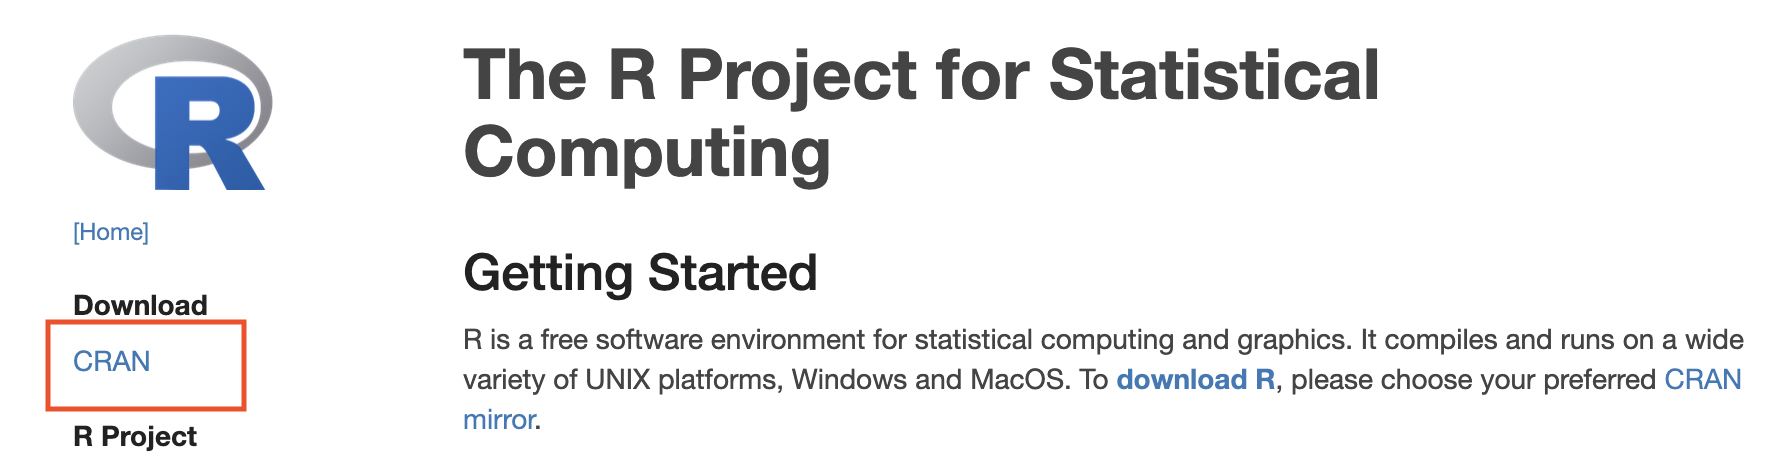
\includegraphics[width=0.75\textwidth,height=\textheight]{./images/CRAN.jpeg}

}

\end{figure}

Here you can select the CRAN mirror. Scroll down until you see USA. You
are free to choose any mirror you like, I recommend using the Duke
University mirror.

\begin{figure}

{\centering 
\includegraphics[width=0.75\textwidth,height=\textheight]{./images/DukeCRAN.jpeg}

}

\end{figure}

Once you click on the hyperlink, you will be prompted to choose the
download for your operating system. Depending on your operating system,
choose either a Windows or Macintosh download.

\begin{figure}

{\centering 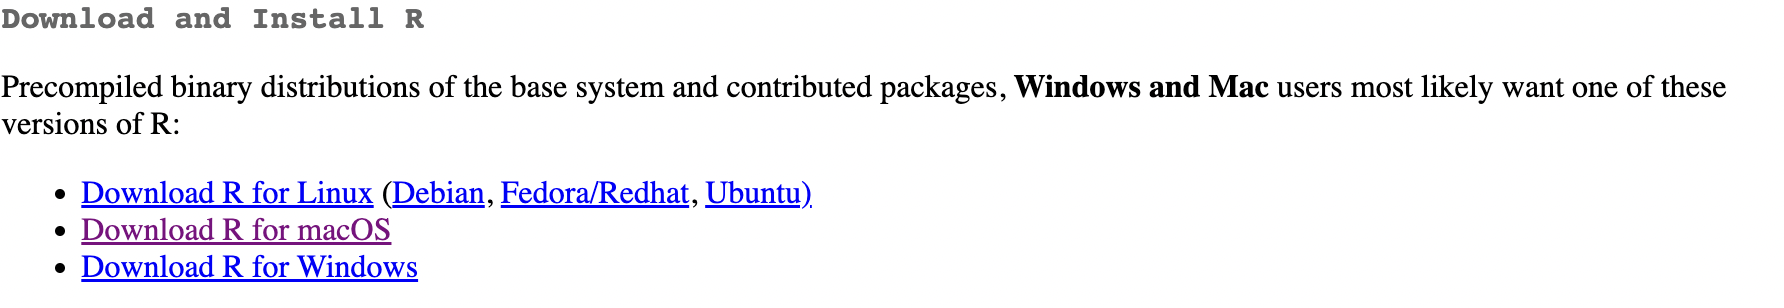
\includegraphics[width=0.75\textwidth,height=\textheight]{./images/OSDownload.jpeg}

}

\end{figure}

Follow all prompts and complete installation.

\hypertarget{installing-rstudio}{%
\section*{Installing RStudio}\label{installing-rstudio}}
\addcontentsline{toc}{section}{Installing RStudio}

\markright{Installing RStudio}

Visit the Posit website at \url{https://posit.co}. Once on the website,
hover to the top right of the screen. You will see a ``Download
RStudio'' blue button.

\begin{figure}

{\centering 
\includegraphics[width=0.75\textwidth,height=\textheight]{./images/RStudio1.jpeg}

}

\end{figure}

Next, scroll down until you reach the RStudio desktop section. Click
once more on ``Download RStudio''. You can now just jump to Step 2 since
you have already downloaded R. Finally, choose the desired download
depending on your operating system.

\begin{figure}

{\centering 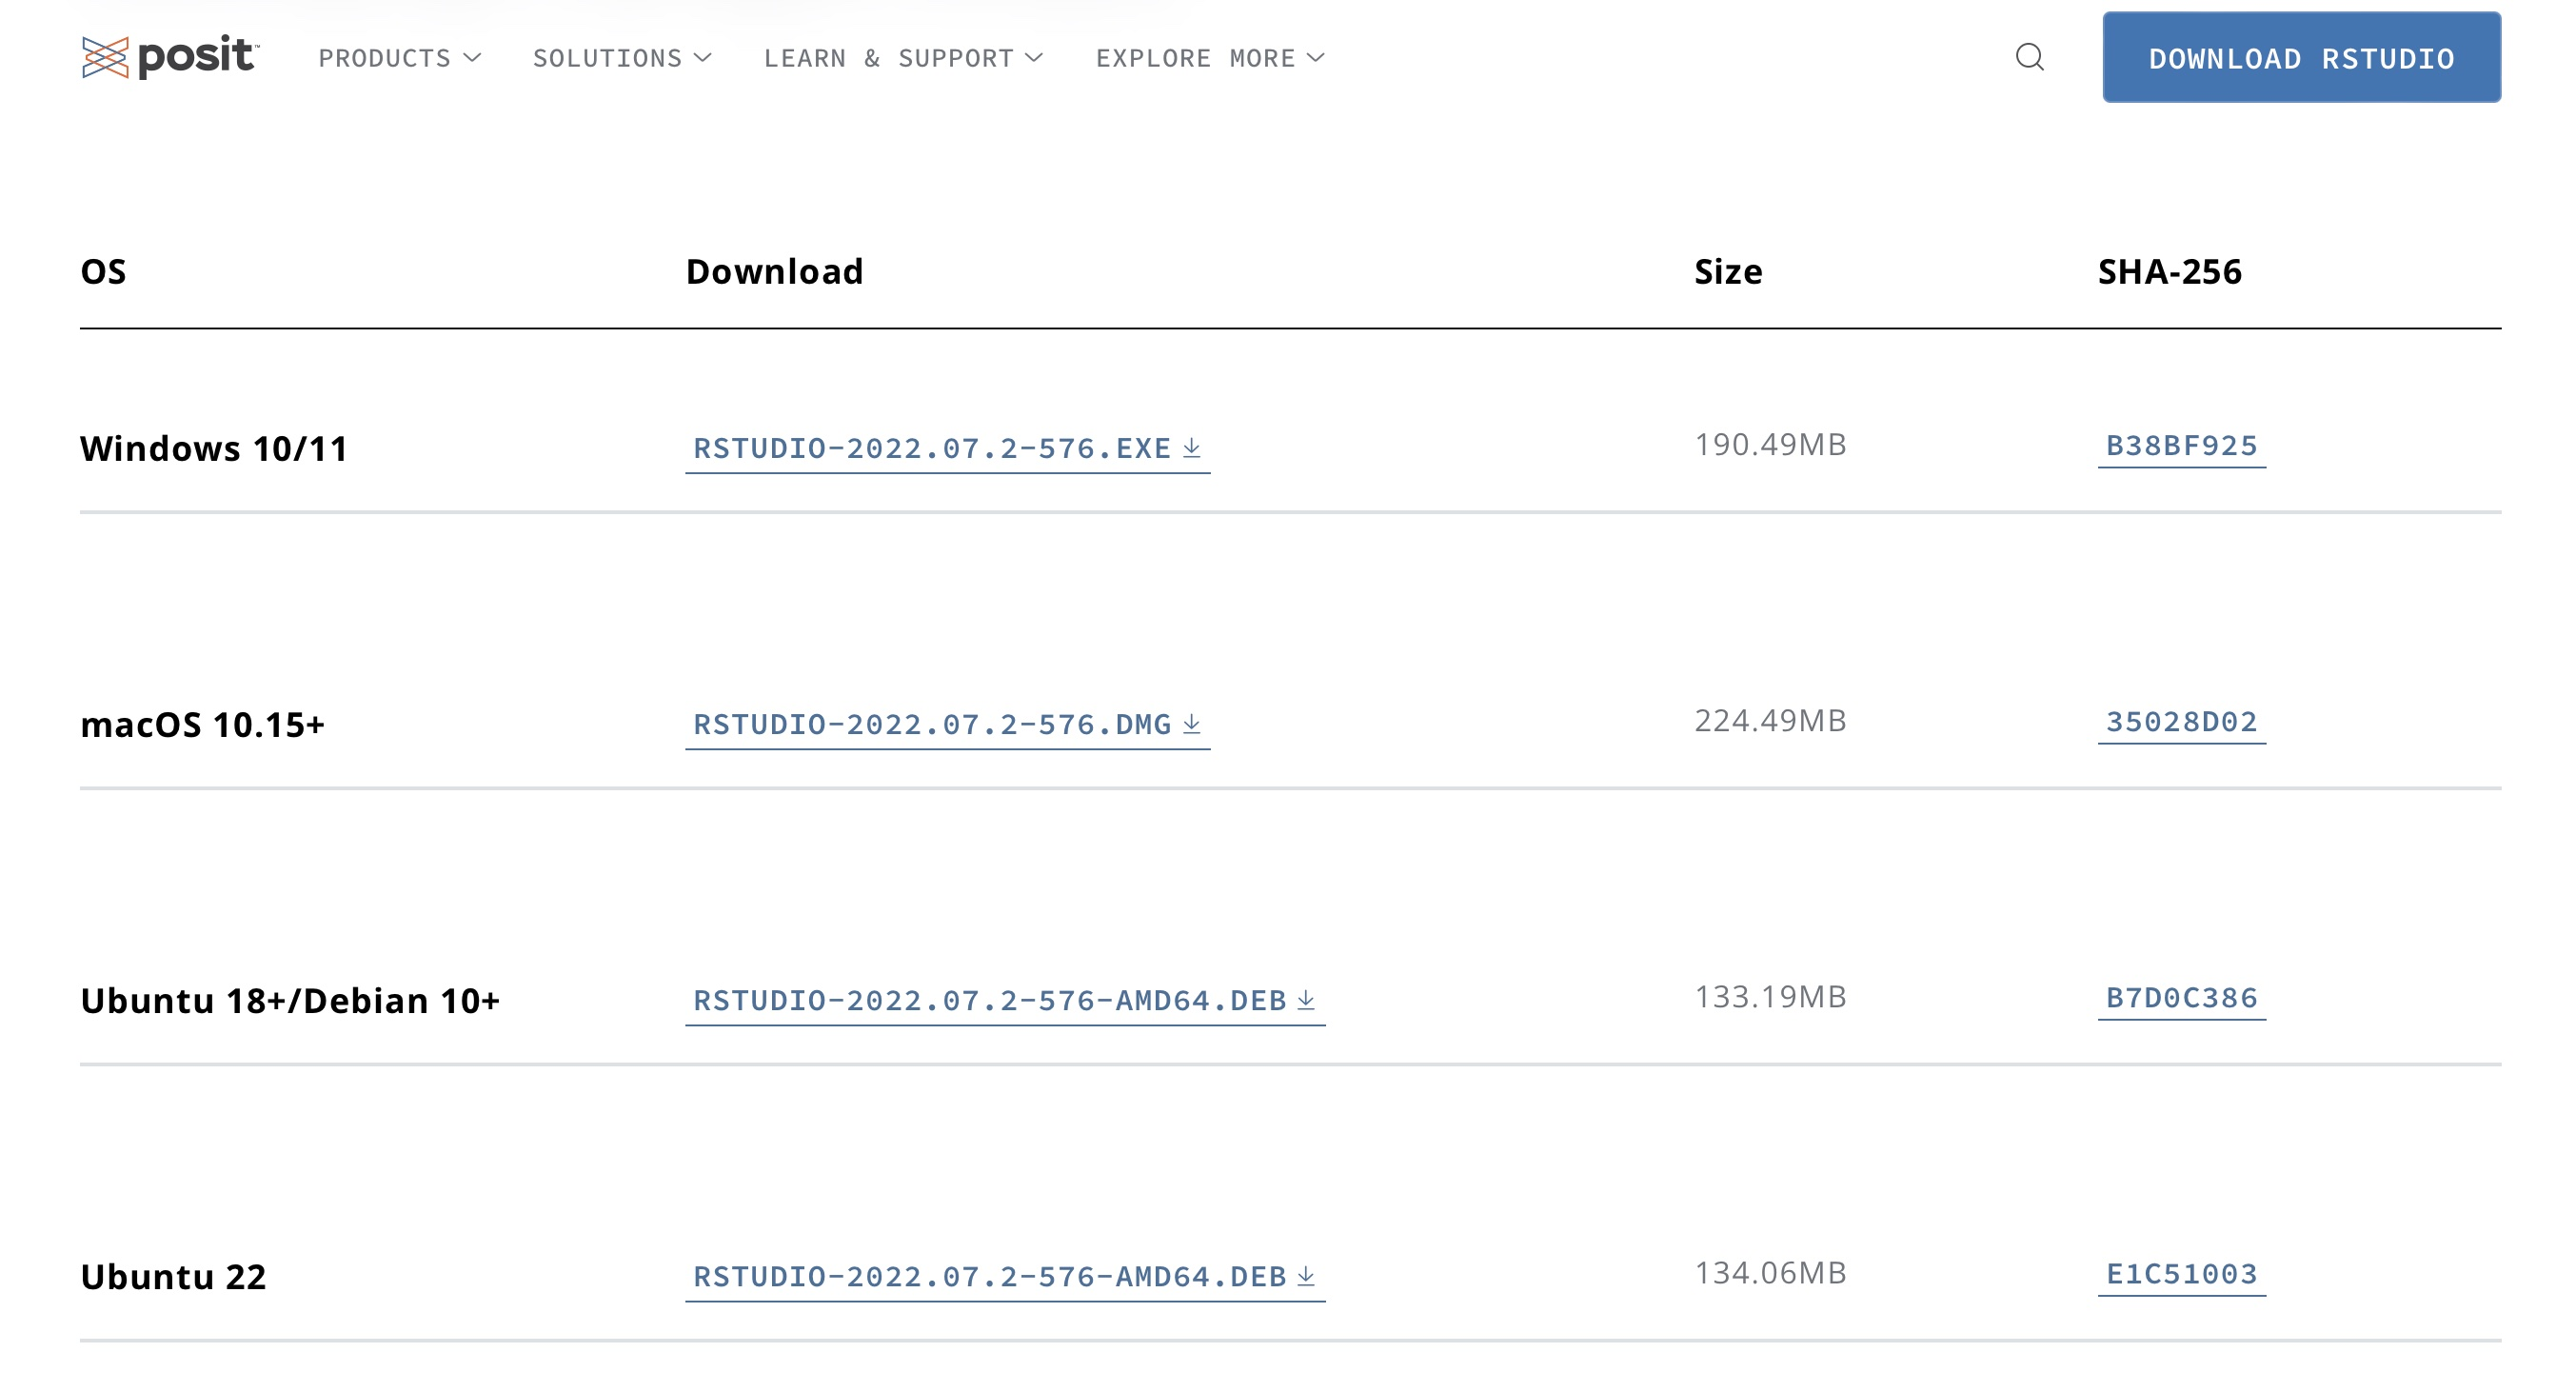
\includegraphics[width=0.75\textwidth,height=\textheight]{./images/Desktop.jpeg}

}

\end{figure}

It is important to note that RStudio will not work if R is not
installed. You can think of R as the engine and RStudio as the
interface.

\hypertarget{posit-cloud}{%
\section*{Posit Cloud}\label{posit-cloud}}
\addcontentsline{toc}{section}{Posit Cloud}

\markright{Posit Cloud}

If you do not wish to install R, you can always use the cloud version.
To do this, visit \url{https://posit.cloud/}. On the main page click on
the ``Sign Up'' button.

\begin{figure}

{\centering 
\includegraphics[width=0.75\textwidth,height=\textheight]{./images/Cloud.jpeg}

}

\end{figure}

Choose the ``Cloud Free'' option and log in using your Google
credentials (if you have a Google account) or sign up if you want to
create a new account.

\part{Descriptive Statistics}

\hypertarget{descriptive-stats-i}{%
\chapter{Descriptive Stats I}\label{descriptive-stats-i}}

\hypertarget{concepts}{%
\section{Concepts}\label{concepts}}

\hypertarget{data-and-types-of-data}{%
\subsection*{Data and Types of Data}\label{data-and-types-of-data}}
\addcontentsline{toc}{subsection}{Data and Types of Data}

\textbf{Data} are facts and figures collected, analyzed and summarized
for presentation and interpretation. Data can be classified as:

\begin{itemize}
\item
  \textbf{Cross Sectional Data} refers to data collected at the same (or
  approximately the same) point in time. Ex: NFL standings in 1980 or
  Country GDP in 2015.
\item
  \textbf{Time Series Data} refers to data collected over several time
  periods. Ex: U.S. inflation rate from 2000-2010 or Tesla deliveries
  from 2016-2022.
\item
  \textbf{Structured Data} resides in a predefined row-column format
  (tidy).
\item
  \textbf{Unstructured Data} do not conform to a pre-defined row-column
  format. Ex: Text, video, and other multimedia.
\end{itemize}

\hypertarget{data-sets-variables-and-scales-of-measurement}{%
\subsection*{Data Sets, Variables and Scales of
Measurement}\label{data-sets-variables-and-scales-of-measurement}}
\addcontentsline{toc}{subsection}{Data Sets, Variables and Scales of
Measurement}

A \textbf{data set} contains all data collected for a particular study.
Data sets are composed of:

\begin{itemize}
\item
  \textbf{Elements} are the entities on which data are collected. Ex:
  Football teams, countries, and individuals.
\item
  \textbf{Observations} are the set of measurements obtained for a
  particular element.
\item
  \textbf{Variables} are a set of characteristics collected for each
  element.
\end{itemize}

The \textbf{scales of measurements} determine the amount and type of
information contained in each variable. In general, variables can be
classified as \textbf{categorical} or \textbf{numerical}.

\begin{itemize}
\item
  \textbf{Categorical} (qualitative) data includes labels or names to
  identify an attribute of each element. Categorical data can be
  \textbf{nominal} or \textbf{ordinal}.

  \begin{itemize}
  \item
    With \textbf{nominal} data, the order of the categories is
    arbitrary. Ex: Marital Status, Race/Ethnicity, or NFL division.
  \item
    With \textbf{ordinal} data, the order or rank of the categories is
    meaningful. Ex: Rating, Difficulty Level, or Spice Level.
  \end{itemize}
\item
  \textbf{Numerical} (quantitative) include numerical values that
  indicate how many (discrete) or how much (continuous). The data can be
  either \textbf{interval} or \textbf{ratio}.

  \begin{itemize}
  \item
    With \textbf{interval} data, the distance between values is
    expressed in terms of a fixed unit of measure. The zero value is
    arbitrary and does not represent the absence of the characteristic.
    Ratios are not meaningful. Ex: Temperature or Dates.
  \item
    With \textbf{ratio} data, the ratio between values is meaningful.
    The zero value is not arbitrary and represents the absence of the
    characteristic. Ex: Prices, Profits, Wins.
  \end{itemize}
\end{itemize}

\hypertarget{useful-r-functions}{%
\subsection*{Useful R Functions}\label{useful-r-functions}}
\addcontentsline{toc}{subsection}{Useful R Functions}

Base R has some important functions that are helpful when dealing with
data. Below is a list that might come handy.

\begin{itemize}
\tightlist
\item
  The \texttt{na.omit()} function removes any observations that have a
  missing value (NA). The resulting data frame has only complete cases.
\item
  The \texttt{nrow()} and \texttt{ncol()} functions return the number of
  rows and columns respectively from a data frame.
\item
  The \texttt{is.na()} function returns a vector of \emph{True} and
  \emph{False} that specify if an entry is missing (NA) or not.
\item
  The \texttt{summary()} function returns a collection of descriptive
  statistics from a data frame (or vector). The function also returns
  whether there are any missing values (NA) in a variable.
\item
  The \texttt{as.integer()}, \texttt{as.factor()}, \texttt{as.double()},
  are functions used to coerce your data into a different scale of
  measurement.
\end{itemize}

The \texttt{dplyr} package has a collection of functions that are useful
for data manipulation and transformation. If you are interested in this
package you can refer to Wickham (2017). To install, run the following
command in the console \texttt{install.packages("dplyr")}.

\begin{itemize}
\tightlist
\item
  The \texttt{arrange()} function allows you to sort data frames in
  ascending order. Pair with the \texttt{desc()} function to sort the
  data in descending order.
\item
  The \texttt{filter()} function allows you to subset the rows of your
  data based on a condition.
\item
  The \texttt{select()} function allows you to select a subset of
  variables from your data frame.
\end{itemize}

\hypertarget{exercises}{%
\section{Exercises}\label{exercises}}

The following exercises will help you test your knowledge on the Scales
of Measurement. They will also allow you to practice some basic data
``wrangling'' in R. In these exercises you will:

\begin{itemize}
\item
  Identify numerical and categorical data.
\item
  Classify data according to their scale of measurement.
\item
  Sort and filter data in R.
\item
  Handle missing values (NA's) in R.
\end{itemize}

Answers are provided below. Try not to peak until you have a formulated
your own answer and double checked your work for any mistakes.

\hypertarget{exercise-1}{%
\subsection*{Exercise 1}\label{exercise-1}}
\addcontentsline{toc}{subsection}{Exercise 1}

A bookstore has compiled data set on their current inventory. A portion
of the data is shown below:

\begin{longtable}[]{@{}cccc@{}}
\toprule()
Title & Price & Year Published & Rating \\
\midrule()
\endhead
Frankenstein & 5.49 & 1818 & 4.2 \\
Dracula & 7.60 & 1897 & 4.0 \\
\ldots{} & \ldots{} & \ldots{} & \ldots{} \\
Sleepy Hollow & 6.95 & 1820 & 3.8 \\
\bottomrule()
\end{longtable}

\begin{enumerate}
\def\labelenumi{\arabic{enumi}.}
\tightlist
\item
  Which of the above variables are categorical and which are numerical?
\item
  What is the measurement scale of each of the above variable?
\end{enumerate}

\hypertarget{exercise-2}{%
\subsection*{Exercise 2}\label{exercise-2}}
\addcontentsline{toc}{subsection}{Exercise 2}

A car company tracks the number of deliveries every quarter. A portion
of the data is shown below:

\begin{longtable}[]{@{}ccc@{}}
\toprule()
Year & Quarter & Deliveries \\
\midrule()
\endhead
2016 & 1 & 14800 \\
2016 & 2 & 14400 \\
\ldots{} & \ldots{} & \ldots{} \\
2022 & 3 & 343840 \\
\bottomrule()
\end{longtable}

\begin{enumerate}
\def\labelenumi{\arabic{enumi}.}
\tightlist
\item
  What is the measurement scale of the Year variable? What are the
  strengths and weaknesses of this type of measurement scale?
\item
  What is the measurement scale for the Quarter variable? What is the
  weakness of this type of measurement scale?
\item
  What is the measurement scale for the Deliveries variable? What are
  the strengths of this type of measurement scale?
\end{enumerate}

\hypertarget{exercise-3}{%
\subsection*{Exercise 3}\label{exercise-3}}
\addcontentsline{toc}{subsection}{Exercise 3}

Use the \textbf{airquality} data set included in R for this problem.

\begin{enumerate}
\def\labelenumi{\arabic{enumi}.}
\tightlist
\item
  Sort the data by \emph{Temp}, \emph{Ozone}, and \emph{Wind} all in
  descending order. What is the day and month of the first observation
  on the sorted data?
\item
  Sort the data only by \emph{Temp} in descending order. Of the \(10\)
  hottest days, how many of them were in July?
\item
  How many missing values are there in the data set? What rows have
  missing values for \emph{Solar.R}?
\item
  Remove all observations that have a missing values. Create a new
  object called \emph{CompleteAG}.
\item
  When using \emph{CompleteAG}, how many days was the temperature at
  least \(60\) degrees?
\item
  When using \emph{CompleteAG}, how many days was the temperature within
  {[}\(55\),\(75\){]} degrees and an \emph{Ozone} below \(20\)?
\end{enumerate}

\hypertarget{answers}{%
\section{Answers}\label{answers}}

\hypertarget{exercise-1-1}{%
\subsection*{Exercise 1}\label{exercise-1-1}}
\addcontentsline{toc}{subsection}{Exercise 1}

\begin{blackbox}

\begin{enumerate}
\def\labelenumi{\arabic{enumi}.}
\tightlist
\item
  The variables Title and Rating are categorical whereas Price and Year
  are numerical.
\end{enumerate}

\end{blackbox}

\begin{blackbox}

\begin{enumerate}
\def\labelenumi{\arabic{enumi}.}
\setcounter{enumi}{1}
\tightlist
\item
  The measurement scale is nominal for Title, ordinal for Ratio, ratio
  for Price, and interval for Year. Recall, that the nominal and ratio
  scales represent the least and most sophisticated levels of
  measurement, respectively.
\end{enumerate}

\end{blackbox}

\hypertarget{exercise-2-1}{%
\subsection*{Exercise 2}\label{exercise-2-1}}
\addcontentsline{toc}{subsection}{Exercise 2}

\begin{blackbox}

\begin{enumerate}
\def\labelenumi{\arabic{enumi}.}
\tightlist
\item
  The variable Year is measured on the interval scale because the
  observations can be ranked, categorized and measured when using this
  kind of scale. However, there is no true zero point so we cannot
  calculate meaningful ratios between years.
\end{enumerate}

\end{blackbox}

\begin{blackbox}

\begin{enumerate}
\def\labelenumi{\arabic{enumi}.}
\setcounter{enumi}{1}
\tightlist
\item
  The variable Quarter is measured on the nominal scale, even though it
  contains numbers. It is the least sophisticated level of measurement
  because if we are presented with nominal data, all we can do is
  categorize or group the data.
\end{enumerate}

\end{blackbox}

\begin{blackbox}

\begin{enumerate}
\def\labelenumi{\arabic{enumi}.}
\setcounter{enumi}{2}
\tightlist
\item
  The variable Deliveries is measured on the ratio scale. It is the
  strongest level of measurement because it allows us to categorize and
  rank the data as well as find meaningful differences between
  observations. Also, with a true zero point, we can interpret the
  ratios between observations.
\end{enumerate}

\end{blackbox}

\hypertarget{exercise-3-1}{%
\subsection*{Exercise 3}\label{exercise-3-1}}
\addcontentsline{toc}{subsection}{Exercise 3}

\begin{blackbox}

\begin{enumerate}
\def\labelenumi{\arabic{enumi}.}
\tightlist
\item
  The day and month of the first observation is August 28th.
\end{enumerate}

\end{blackbox}

The easiest way to sort in R is by using the \texttt{dplyr} package.
Specifically, the \texttt{arrange()} function within the package. Let's
also use the \texttt{desc()} function to make sure that the data is
sorted in descending order. We can use indexing to retrieve the first
row of the sorted data set.

\begin{Shaded}
\begin{Highlighting}[numbers=left,,]
\FunctionTok{library}\NormalTok{(dplyr)}
\NormalTok{SortedAQ}\OtherTok{\textless{}{-}}\FunctionTok{arrange}\NormalTok{(airquality,}\FunctionTok{desc}\NormalTok{(Temp),}\FunctionTok{desc}\NormalTok{(Ozone),}\FunctionTok{desc}\NormalTok{(Wind))}
\NormalTok{SortedAQ[}\DecValTok{1}\NormalTok{,]}
\end{Highlighting}
\end{Shaded}

\begin{verbatim}
  Ozone Solar.R Wind Temp Month Day
1    76     203  9.7   97     8  28
\end{verbatim}

\begin{blackbox}

\begin{enumerate}
\def\labelenumi{\arabic{enumi}.}
\setcounter{enumi}{1}
\tightlist
\item
  Of the \(10\) hottest days only two were in July.
\end{enumerate}

\end{blackbox}

We can use the \texttt{arrange()} function one more time for this
question. Then we can use indexing to retrieve the top \(10\)
observations.

\begin{Shaded}
\begin{Highlighting}[numbers=left,,]
\NormalTok{SortedAQ2}\OtherTok{\textless{}{-}}\FunctionTok{arrange}\NormalTok{(airquality,}\FunctionTok{desc}\NormalTok{(Temp))}
\NormalTok{SortedAQ2[}\DecValTok{1}\SpecialCharTok{:}\DecValTok{10}\NormalTok{,]}
\end{Highlighting}
\end{Shaded}

\begin{verbatim}
   Ozone Solar.R Wind Temp Month Day
1     76     203  9.7   97     8  28
2     84     237  6.3   96     8  30
3    118     225  2.3   94     8  29
4     85     188  6.3   94     8  31
5     NA     259 10.9   93     6  11
6     73     183  2.8   93     9   3
7     91     189  4.6   93     9   4
8     NA     250  9.2   92     6  12
9     97     267  6.3   92     7   8
10    97     272  5.7   92     7   9
\end{verbatim}

\begin{blackbox}

\begin{enumerate}
\def\labelenumi{\arabic{enumi}.}
\setcounter{enumi}{2}
\tightlist
\item
  There are a total of \(44\) missing values. \emph{Ozone} has \(37\)
  and \emph{Solar.R} has \(7\). Rows \(5\), \(6\), \(11\), \(27\),
  \(96\), \(97\), \(98\) are missing for \emph{Solar.R}.
\end{enumerate}

\end{blackbox}

We can easily identify missing values with the \texttt{summary()}
function.

\begin{Shaded}
\begin{Highlighting}[numbers=left,,]
\FunctionTok{summary}\NormalTok{(airquality)}
\end{Highlighting}
\end{Shaded}

\begin{verbatim}
     Ozone           Solar.R           Wind             Temp      
 Min.   :  1.00   Min.   :  7.0   Min.   : 1.700   Min.   :56.00  
 1st Qu.: 18.00   1st Qu.:115.8   1st Qu.: 7.400   1st Qu.:72.00  
 Median : 31.50   Median :205.0   Median : 9.700   Median :79.00  
 Mean   : 42.13   Mean   :185.9   Mean   : 9.958   Mean   :77.88  
 3rd Qu.: 63.25   3rd Qu.:258.8   3rd Qu.:11.500   3rd Qu.:85.00  
 Max.   :168.00   Max.   :334.0   Max.   :20.700   Max.   :97.00  
 NA's   :37       NA's   :7                                       
     Month            Day      
 Min.   :5.000   Min.   : 1.0  
 1st Qu.:6.000   1st Qu.: 8.0  
 Median :7.000   Median :16.0  
 Mean   :6.993   Mean   :15.8  
 3rd Qu.:8.000   3rd Qu.:23.0  
 Max.   :9.000   Max.   :31.0  
                               
\end{verbatim}

To view the rows that have NA's in them, we can use the \texttt{is.na()}
function and indexing. Below we see that \(7\) values are missing for
the \emph{Solar.R} variable in the months \(5\) and \(8\) combined.

\begin{Shaded}
\begin{Highlighting}[numbers=left,,]
\NormalTok{airquality[}\FunctionTok{is.na}\NormalTok{(airquality}\SpecialCharTok{$}\NormalTok{Solar.R),]}
\end{Highlighting}
\end{Shaded}

\begin{verbatim}
   Ozone Solar.R Wind Temp Month Day
5     NA      NA 14.3   56     5   5
6     28      NA 14.9   66     5   6
11     7      NA  6.9   74     5  11
27    NA      NA  8.0   57     5  27
96    78      NA  6.9   86     8   4
97    35      NA  7.4   85     8   5
98    66      NA  4.6   87     8   6
\end{verbatim}

\begin{blackbox}

\begin{enumerate}
\def\labelenumi{\arabic{enumi}.}
\setcounter{enumi}{3}
\tightlist
\item
  To create the new object of complete observations we can use the
  \texttt{na.omit()} function.
\end{enumerate}

\end{blackbox}

\begin{Shaded}
\begin{Highlighting}[numbers=left,,]
\NormalTok{CompleteAQ}\OtherTok{\textless{}{-}}\FunctionTok{na.omit}\NormalTok{(airquality)}
\end{Highlighting}
\end{Shaded}

\begin{blackbox}

\begin{enumerate}
\def\labelenumi{\arabic{enumi}.}
\setcounter{enumi}{4}
\tightlist
\item
  There were \(107\) days where the temperature was at least \(60\).
\end{enumerate}

\end{blackbox}

Using base R we have:

\begin{Shaded}
\begin{Highlighting}[numbers=left,,]
\FunctionTok{nrow}\NormalTok{(CompleteAQ[CompleteAQ}\SpecialCharTok{$}\NormalTok{Temp}\SpecialCharTok{\textgreater{}=}\DecValTok{60}\NormalTok{,])}
\end{Highlighting}
\end{Shaded}

\begin{verbatim}
[1] 107
\end{verbatim}

We can also use \texttt{dplyr} for this question. Specifically, using
the \texttt{filter()} and \texttt{nrow()} functions we get:

\begin{Shaded}
\begin{Highlighting}[numbers=left,,]
\FunctionTok{nrow}\NormalTok{(}\FunctionTok{filter}\NormalTok{(CompleteAQ,Temp}\SpecialCharTok{\textgreater{}=}\DecValTok{60}\NormalTok{))}
\end{Highlighting}
\end{Shaded}

\begin{verbatim}
[1] 107
\end{verbatim}

\begin{blackbox}

\begin{enumerate}
\def\labelenumi{\arabic{enumi}.}
\setcounter{enumi}{5}
\tightlist
\item
  There were \(24\) days where the temperature was between \(55\) and
  \(75\) and the ozone level was below \(20\).
\end{enumerate}

\end{blackbox}

Using base R we have:

\begin{Shaded}
\begin{Highlighting}[numbers=left,,]
\FunctionTok{nrow}\NormalTok{(CompleteAQ[CompleteAQ}\SpecialCharTok{$}\NormalTok{Temp}\SpecialCharTok{\textgreater{}}\DecValTok{55} \SpecialCharTok{\&}\NormalTok{ CompleteAQ}\SpecialCharTok{$}\NormalTok{Temp}\SpecialCharTok{\textless{}}\DecValTok{75} \SpecialCharTok{\&}\NormalTok{ CompleteAQ}\SpecialCharTok{$}\NormalTok{Ozone}\SpecialCharTok{\textless{}}\DecValTok{20}\NormalTok{,])}
\end{Highlighting}
\end{Shaded}

\begin{verbatim}
[1] 24
\end{verbatim}

Using the \texttt{filter()} function once more we get:

\begin{Shaded}
\begin{Highlighting}[numbers=left,,]
\FunctionTok{nrow}\NormalTok{(}\FunctionTok{filter}\NormalTok{(CompleteAQ,Temp}\SpecialCharTok{\textgreater{}}\DecValTok{55}\NormalTok{,Temp}\SpecialCharTok{\textless{}}\DecValTok{75}\NormalTok{,Ozone}\SpecialCharTok{\textless{}}\DecValTok{20}\NormalTok{))}
\end{Highlighting}
\end{Shaded}

\begin{verbatim}
[1] 24
\end{verbatim}

\hypertarget{descriptive-stats-ii}{%
\chapter{Descriptive Stats II}\label{descriptive-stats-ii}}

\hypertarget{concepts-1}{%
\section{Concepts}\label{concepts-1}}

\hypertarget{frequency}{%
\subsection*{Frequency}\label{frequency}}
\addcontentsline{toc}{subsection}{Frequency}

A \textbf{frequency distribution} is a tabular summary of data showing
the number of items in each of several non-overlapping classes.

\begin{itemize}
\tightlist
\item
  The \textbf{relative frequency} is calculated by \(f_{i}/n\), where
  \(f_{i}\) is the frequency of class \(i\) and \(n\) is the total
  frequency.
\item
  The \textbf{cumulative frequency} shows the number of data items with
  values less than or equal to the upper class limit of each class.
\item
  The \textbf{cumulative relative frequency} is given by \(cf_{i}/n\),
  where \(cf_{i}\) is the cumulative frequency of class \(i\).
\end{itemize}

\hypertarget{plots}{%
\subsection*{Plots}\label{plots}}
\addcontentsline{toc}{subsection}{Plots}

A \textbf{bar plot} illustrates the frequency distribution of
qualitative data.

\begin{itemize}
\item
  Is an illustration for qualitative data.
\item
  Includes the classes in the horizontal axis and frequencies or
  relative frequencies in the vertical axis.
\item
  Has gaps between each bar.
\end{itemize}

A \textbf{histogram} illustrates the frequency distribution of
quantitative data.

\begin{itemize}
\item
  Is an illustration for quantitative data.
\item
  There are no gaps between the bars.
\item
  The \textbf{number}, \textbf{width} and \textbf{limits} of each class
  must be determined.

  \begin{itemize}
  \tightlist
  \item
    The \textbf{number} of classes can be determined by the \(2^k\)
    rule: select \(k\) such that \(2^k\) is greater than the number of
    observations by the smallest amount.
  \item
    The \textbf{width} of the class is approximately \emph{range/(\# of
    Classes)}. The value should be rounded up.
  \item
    The \textbf{limits} should be chosen so that each point belongs to
    only one class.
  \end{itemize}
\end{itemize}

\hypertarget{useful-r-functions-1}{%
\subsection*{Useful R Functions}\label{useful-r-functions-1}}
\addcontentsline{toc}{subsection}{Useful R Functions}

The \texttt{table()} command generates frequency distributions or
contingency tables if two variables are used.

The \texttt{prop.table()} command generates relative frequency
distributions from an object that contains a table.

The \texttt{cut()} function generates class limits and bins used in
frequency distributions (and histograms) for quantitative data.

Base R has the \texttt{barplot()} function for categorical variable,
\texttt{histogram()} function for numerical data, and the
\texttt{plot()} function for line charts or scatter plots. Below are
some arguments that are helpful when plotting.

\begin{itemize}
\tightlist
\item
  \emph{main}: used to set the plot's title. The title should be entered
  as a character.
\item
  \emph{col}: used to set the color of the plot. Hex and RGB values are
  allowed as inputs. The color should be entered as a character.
\item
  \emph{xlab} and \emph{ylab}: are used to set the labels for the \(x\)
  and \(y\) axis respectively. The labels should be entered as
  characters.
\item
  \texttt{legend()} is a function to customize the legend of a graph.
  This argument may be used with the \texttt{plot()}, \texttt{barplot()}
  or \texttt{histogram()} functions.

  \begin{itemize}
  \tightlist
  \item
    \emph{x}: used to set the location of the legend in the plotting
    area. Ex: ``bottomleft''.
  \item
    \emph{legend}: a vector specifying the legend names to be included.
  \item
    \emph{col}: a vector specifying the color of each item in the
    legend.
  \end{itemize}
\end{itemize}

\hypertarget{exercises-1}{%
\section{Exercises}\label{exercises-1}}

The following exercises will help you practice summarizing data with
tables and simple graphs. In particular, the exercises work on:

\begin{itemize}
\item
  Developing frequency distributions for both categorical and numerical
  data.
\item
  Constructing bar charts, histograms, and line charts.
\item
  Creating contingency tables.
\end{itemize}

Answers are provided below. Try not to peak until you have a formulated
your own answer and double checked your work for any mistakes.

\hypertarget{exercise-1-2}{%
\subsection*{Exercise 1}\label{exercise-1-2}}
\addcontentsline{toc}{subsection}{Exercise 1}

Install the \texttt{ISLR2} package in R. You will need the
\textbf{BrainCancer} data set to answer this question.

\begin{enumerate}
\def\labelenumi{\arabic{enumi}.}
\tightlist
\item
  Construct a frequency and relative frequency table of the
  \emph{Diagnosis} variable. What was the most common diagnosis? What
  percentage of the sample had this diagnosis?
\item
  Construct a bar chart. Summarize the findings.
\item
  Construct a contingency table that shows the \emph{Diagnosis} along
  with the \emph{Status}. Which diagnosis had the highest number of
  non-survivals (0)? What was the survival rate of this diagnosis?
\item
  Construct a stacked column chart. Which two \emph{Diagnosis} and
  \emph{Status} combinations are the most frequent?
\end{enumerate}

\hypertarget{exercise-2-2}{%
\subsection*{Exercise 2}\label{exercise-2-2}}
\addcontentsline{toc}{subsection}{Exercise 2}

You will need the \textbf{airquality} data set (in base R) to answer
this question.

\begin{enumerate}
\def\labelenumi{\arabic{enumi}.}
\tightlist
\item
  Construct a frequency distribution for \emph{Temp}. Use five intervals
  with widths of \(50<x\le60\); \(60<x\le70\); etc. Which interval had
  the highest frequency? How many times was the temperature between
  \(50\) and \(60\) degrees?
\item
  Construct a relative frequency, cumulative frequency and the relative
  cumulative frequency distributions. What proportion of the time was
  \emph{Temp} between \(50\) and \(60\) degrees? How many times was the
  \emph{Temp} \(70\) degrees or less? What proportion of the time was
  \emph{Temp} more than \(70\) degrees?
\item
  Construct the histogram. Is the distribution symmetric? If not, is it
  skewed to the left or right?
\end{enumerate}

\hypertarget{exercise-3-2}{%
\subsection*{Exercise 3}\label{exercise-3-2}}
\addcontentsline{toc}{subsection}{Exercise 3}

You will need the \textbf{Portfolio} data set from the \texttt{ISLR2}
package to answer this question.

\begin{enumerate}
\def\labelenumi{\arabic{enumi}.}
\tightlist
\item
  Construct a line chart that shows the returns over time for each
  portfolio (X and Y) by using two lines each with a unique color.
  Assume the data is for the period \(1901\) to \(2000\). Include also a
  legend that matches colors to portfolios.
\end{enumerate}

\hypertarget{answers-1}{%
\section{Answers}\label{answers-1}}

\hypertarget{exercise-1-3}{%
\subsection*{Exercise 1}\label{exercise-1-3}}
\addcontentsline{toc}{subsection}{Exercise 1}

\begin{blackbox}

\begin{enumerate}
\def\labelenumi{\arabic{enumi}.}
\tightlist
\item
  The most common diagnosis is Meningioma, a slow-growing tumor that
  forms from the membranous layers surrounding the brain and spinal
  cord. The diagnosis represents about \(48.28\)\% of the sample.
\end{enumerate}

\end{blackbox}

Start by loading the \texttt{ISLR2} package. To construct the frequency
distribution table, use the \texttt{table()} function.

\begin{Shaded}
\begin{Highlighting}[numbers=left,,]
\FunctionTok{library}\NormalTok{(ISLR2)}
\FunctionTok{table}\NormalTok{(BrainCancer}\SpecialCharTok{$}\NormalTok{diagnosis)}
\end{Highlighting}
\end{Shaded}

\begin{verbatim}

Meningioma  LG glioma  HG glioma      Other 
        42          9         22         14 
\end{verbatim}

The relative frequency distribution can be easily retrieved by saving
the frequency table in an object and then using the
\texttt{prop.table()} function.

\begin{Shaded}
\begin{Highlighting}[numbers=left,,]
\NormalTok{freq}\OtherTok{\textless{}{-}}\FunctionTok{table}\NormalTok{(BrainCancer}\SpecialCharTok{$}\NormalTok{diagnosis)}
\FunctionTok{prop.table}\NormalTok{(freq)}
\end{Highlighting}
\end{Shaded}

\begin{verbatim}

Meningioma  LG glioma  HG glioma      Other 
 0.4827586  0.1034483  0.2528736  0.1609195 
\end{verbatim}

\begin{blackbox}

\begin{enumerate}
\def\labelenumi{\arabic{enumi}.}
\setcounter{enumi}{1}
\tightlist
\item
  The majority of diagnosis are Meningioma. Low grade glioma is the
  least common of diagnosis. High grade glioma and other diagnosis have
  about the same frequency.
\end{enumerate}

\end{blackbox}

To construct the bar chart use the \texttt{barplot()} function in R.

\begin{Shaded}
\begin{Highlighting}[numbers=left,,]
\FunctionTok{barplot}\NormalTok{(freq, }\AttributeTok{col =} \StringTok{"\#F5F5F5"}\NormalTok{, }\AttributeTok{ylim=}\FunctionTok{c}\NormalTok{(}\DecValTok{0}\NormalTok{,}\DecValTok{50}\NormalTok{))}
\end{Highlighting}
\end{Shaded}

\begin{figure}[H]

{\centering 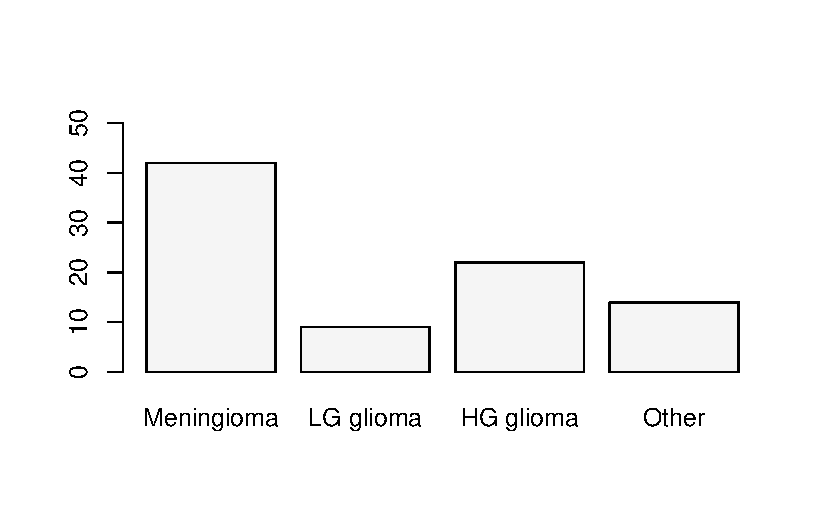
\includegraphics{./03-DescriptiveII_files/figure-pdf/unnamed-chunk-3-1.pdf}

}

\end{figure}

\begin{blackbox}

\begin{enumerate}
\def\labelenumi{\arabic{enumi}.}
\setcounter{enumi}{2}
\tightlist
\item
  \(33\) people did not survive Meningioma. The survival rate of
  Meningioma is only \(21.43\)\%.
\end{enumerate}

\end{blackbox}

Use the \texttt{table()} function one more time to create the
contingency table for the two variables.

\begin{Shaded}
\begin{Highlighting}[numbers=left,,]
\NormalTok{(freq2}\OtherTok{\textless{}{-}}\FunctionTok{table}\NormalTok{(BrainCancer}\SpecialCharTok{$}\NormalTok{status,BrainCancer}\SpecialCharTok{$}\NormalTok{diagnosis))}
\end{Highlighting}
\end{Shaded}

\begin{verbatim}
   
    Meningioma LG glioma HG glioma Other
  0         33         5         5     9
  1          9         4        17     5
\end{verbatim}

To get the survival rates, we can use the \texttt{prop.table()} function
once again.

\begin{Shaded}
\begin{Highlighting}[numbers=left,,]
\FunctionTok{prop.table}\NormalTok{(freq2,}\AttributeTok{margin =} \DecValTok{2}\NormalTok{)}
\end{Highlighting}
\end{Shaded}

\begin{verbatim}
   
    Meningioma LG glioma HG glioma     Other
  0  0.7857143 0.5555556 0.2272727 0.6428571
  1  0.2142857 0.4444444 0.7727273 0.3571429
\end{verbatim}

\begin{blackbox}

\begin{enumerate}
\def\labelenumi{\arabic{enumi}.}
\setcounter{enumi}{3}
\tightlist
\item
  Meningioma and not surviving is the most common with \(33\)
  occurrences. High grade glioma and surviving is the the second most
  common.
\end{enumerate}

\end{blackbox}

Use the \texttt{barplot()} function one more time to construct the
stacked column chart.

\begin{Shaded}
\begin{Highlighting}[numbers=left,,]
\FunctionTok{barplot}\NormalTok{(}\FunctionTok{table}\NormalTok{(BrainCancer}\SpecialCharTok{$}\NormalTok{status,BrainCancer}\SpecialCharTok{$}\NormalTok{diagnosis),}
        \AttributeTok{legend.text =} \FunctionTok{c}\NormalTok{(}\StringTok{"Not Survived"}\NormalTok{,}\StringTok{"Survived"}\NormalTok{), }\AttributeTok{ylim=}\FunctionTok{c}\NormalTok{(}\DecValTok{0}\NormalTok{,}\DecValTok{50}\NormalTok{))}
\end{Highlighting}
\end{Shaded}

\begin{figure}[H]

{\centering 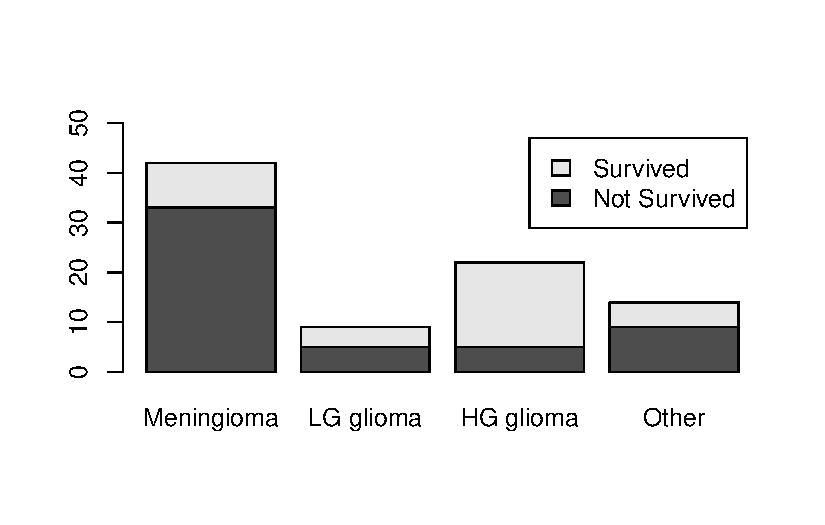
\includegraphics{./03-DescriptiveII_files/figure-pdf/unnamed-chunk-6-1.pdf}

}

\end{figure}

\hypertarget{exercise-2-3}{%
\subsection*{Exercise 2}\label{exercise-2-3}}
\addcontentsline{toc}{subsection}{Exercise 2}

\begin{blackbox}

\begin{enumerate}
\def\labelenumi{\arabic{enumi}.}
\tightlist
\item
  The highest frequency is in the \(80 < x ≤ 90\) bin. \(8\)
  temperatures were between \(50 < x ≤ 60\) degrees.
\end{enumerate}

\end{blackbox}

Create a vector containing the intervals desired by using the
\texttt{seq()} function.

\begin{Shaded}
\begin{Highlighting}[numbers=left,,]
\NormalTok{intervals }\OtherTok{\textless{}{-}} \FunctionTok{seq}\NormalTok{(}\DecValTok{50}\NormalTok{, }\DecValTok{100}\NormalTok{, }\AttributeTok{by=}\DecValTok{10}\NormalTok{)}
\end{Highlighting}
\end{Shaded}

Next use the \texttt{cut()} function to create the cuts for the
histogram.

\begin{Shaded}
\begin{Highlighting}[numbers=left,,]
\NormalTok{intervals.cut }\OtherTok{\textless{}{-}} \FunctionTok{cut}\NormalTok{(airquality}\SpecialCharTok{$}\NormalTok{Temp, intervals, }\AttributeTok{left=}\ConstantTok{FALSE}\NormalTok{, }\AttributeTok{right=}\ConstantTok{TRUE}\NormalTok{)}
\end{Highlighting}
\end{Shaded}

The frequency distribution can be obtained by using the \texttt{table()}
function on the \emph{interval.cut} object created above.

\begin{Shaded}
\begin{Highlighting}[numbers=left,,]
\FunctionTok{table}\NormalTok{(intervals.cut)}
\end{Highlighting}
\end{Shaded}

\begin{verbatim}
intervals.cut
 (50,60]  (60,70]  (70,80]  (80,90] (90,100] 
       8       25       52       54       14 
\end{verbatim}

\begin{blackbox}

\begin{enumerate}
\def\labelenumi{\arabic{enumi}.}
\setcounter{enumi}{1}
\tightlist
\item
  The temperature was \(5.22\)\% of the time between \(50\) and \(60\);
  The temperature was \(70\) or less \(33\) times; The temperature was
  above \(70\), \(78.43\)\% of the time.
\end{enumerate}

\end{blackbox}

To get the relative frequency table, start by saving the proportion
table into an object.Then you can use the \texttt{prop.table()}
function.

\begin{Shaded}
\begin{Highlighting}[numbers=left,,]
\NormalTok{freq}\OtherTok{\textless{}{-}}\FunctionTok{table}\NormalTok{(intervals.cut) }
\FunctionTok{prop.table}\NormalTok{(freq)}
\end{Highlighting}
\end{Shaded}

\begin{verbatim}
intervals.cut
   (50,60]    (60,70]    (70,80]    (80,90]   (90,100] 
0.05228758 0.16339869 0.33986928 0.35294118 0.09150327 
\end{verbatim}

For the cumulative distribution you can use the \texttt{cumsum()}
function on the frequency distribution.

\begin{Shaded}
\begin{Highlighting}[numbers=left,,]
\NormalTok{cumulfreq}\OtherTok{\textless{}{-}}\FunctionTok{cumsum}\NormalTok{(freq)}
\NormalTok{cumulfreq}
\end{Highlighting}
\end{Shaded}

\begin{verbatim}
 (50,60]  (60,70]  (70,80]  (80,90] (90,100] 
       8       33       85      139      153 
\end{verbatim}

Lastly, for the relative cumulative distribution table, you can use the
\texttt{cumsum()} function on the relative frequency table.

\begin{Shaded}
\begin{Highlighting}[numbers=left,,]
\FunctionTok{cumsum}\NormalTok{(}\FunctionTok{prop.table}\NormalTok{(freq))}
\end{Highlighting}
\end{Shaded}

\begin{verbatim}
   (50,60]    (60,70]    (70,80]    (80,90]   (90,100] 
0.05228758 0.21568627 0.55555556 0.90849673 1.00000000 
\end{verbatim}

\begin{blackbox}

\begin{enumerate}
\def\labelenumi{\arabic{enumi}.}
\setcounter{enumi}{2}
\tightlist
\item
  The distribution is not perfectly symmetric. It is skewed slightly to
  the left (see histogram.)
\end{enumerate}

\end{blackbox}

Use the \texttt{hist()} function to create the histogram.

\begin{Shaded}
\begin{Highlighting}[numbers=left,,]
\FunctionTok{hist}\NormalTok{(airquality}\SpecialCharTok{$}\NormalTok{Temp, }\AttributeTok{breaks=}\NormalTok{intervals, }
     \AttributeTok{right=}\ConstantTok{TRUE}\NormalTok{,}\AttributeTok{col=}\StringTok{"\#F5F5F5"}\NormalTok{, }\AttributeTok{main=}\StringTok{"Temperature in NY"}\NormalTok{, }\AttributeTok{xlab=}\StringTok{""}\NormalTok{)}
\end{Highlighting}
\end{Shaded}

\begin{figure}[H]

{\centering 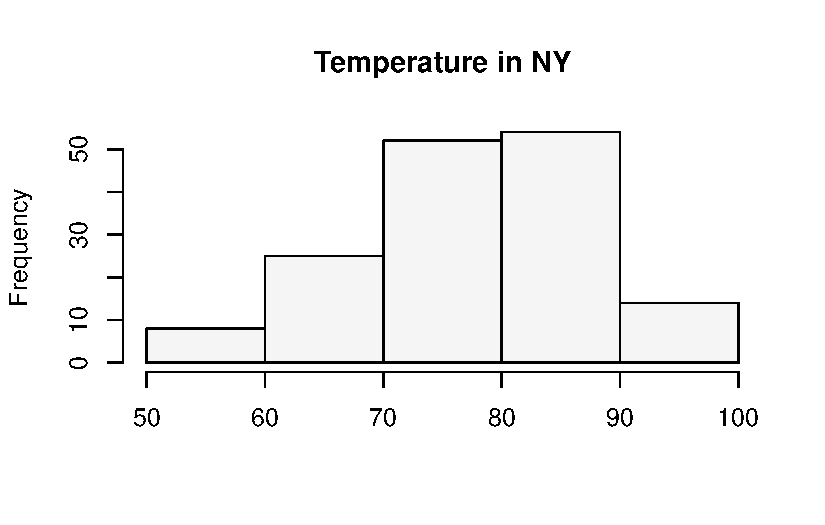
\includegraphics{./03-DescriptiveII_files/figure-pdf/unnamed-chunk-13-1.pdf}

}

\end{figure}

\hypertarget{exercise-3-3}{%
\subsection*{Exercise 3}\label{exercise-3-3}}
\addcontentsline{toc}{subsection}{Exercise 3}

\begin{blackbox}

\begin{enumerate}
\def\labelenumi{\arabic{enumi}.}
\tightlist
\item
  From \(1901\) through \(2000\), both portfolios have behaved very
  similarly. Returns are between \(-3\)\% and \(3\)\%, there is no
  trend, and positive (negative) returns for X seem to match with
  positive (negative) returns of Y.
\end{enumerate}

\end{blackbox}

You can use the \texttt{plot()} function to create a plot of Portfolio
Y. The line for Portfolio X can be added with the \texttt{lines()}
function.

\begin{Shaded}
\begin{Highlighting}[numbers=left,,]
\FunctionTok{plot}\NormalTok{(Portfolio}\SpecialCharTok{$}\NormalTok{Y, }
     \AttributeTok{x=}\FunctionTok{seq}\NormalTok{(}\DecValTok{1901}\NormalTok{,}\DecValTok{2000}\NormalTok{), }\AttributeTok{type=}\StringTok{"l"}\NormalTok{, }
     \AttributeTok{col=}\StringTok{"black"}\NormalTok{, }\AttributeTok{xlab=}\StringTok{""}\NormalTok{, }\AttributeTok{ylab=}\StringTok{"\% Return"}\NormalTok{, }\AttributeTok{ylim=}\FunctionTok{c}\NormalTok{(}\SpecialCharTok{{-}}\DecValTok{3}\NormalTok{,}\DecValTok{3}\NormalTok{), }
     \AttributeTok{xlim=}\FunctionTok{c}\NormalTok{(}\DecValTok{1901}\NormalTok{,}\DecValTok{2000}\NormalTok{), }\AttributeTok{lwd=}\DecValTok{2}\NormalTok{, }\AttributeTok{axes =}\NormalTok{ F)}
\FunctionTok{axis}\NormalTok{(}\AttributeTok{side=}\DecValTok{1}\NormalTok{, }\AttributeTok{labels=}\ConstantTok{TRUE}\NormalTok{, }\AttributeTok{font=}\DecValTok{1}\NormalTok{,}\AttributeTok{las=}\DecValTok{1}\NormalTok{)}
\FunctionTok{axis}\NormalTok{(}\AttributeTok{side=}\DecValTok{2}\NormalTok{, }\AttributeTok{labels=}\ConstantTok{TRUE}\NormalTok{, }\AttributeTok{font=}\DecValTok{1}\NormalTok{,}\AttributeTok{las=}\DecValTok{1}\NormalTok{)}
\FunctionTok{lines}\NormalTok{(Portfolio}\SpecialCharTok{$}\NormalTok{X, }\AttributeTok{x=}\FunctionTok{seq}\NormalTok{(}\DecValTok{1901}\NormalTok{,}\DecValTok{2000}\NormalTok{), }\AttributeTok{type=}\StringTok{"l"}\NormalTok{, }
      \AttributeTok{col=}\StringTok{"darkgrey"}\NormalTok{, }\AttributeTok{lwd=}\DecValTok{2}\NormalTok{)}
\FunctionTok{legend}\NormalTok{(}\AttributeTok{x =} \StringTok{"bottomleft"}\NormalTok{,          }
       \AttributeTok{legend =} \FunctionTok{c}\NormalTok{(}\StringTok{"Port Y"}\NormalTok{, }\StringTok{"Port X"}\NormalTok{),  }
       \AttributeTok{lty =} \FunctionTok{c}\NormalTok{(}\DecValTok{1}\NormalTok{, }\DecValTok{1}\NormalTok{),           }
       \AttributeTok{col =} \FunctionTok{c}\NormalTok{(}\StringTok{"black"}\NormalTok{, }\StringTok{"darkgrey"}\NormalTok{),         }
       \AttributeTok{lwd =} \DecValTok{2}\NormalTok{,}
       \AttributeTok{bty=}\StringTok{"n"}\NormalTok{)                }
\end{Highlighting}
\end{Shaded}

\begin{figure}[H]

{\centering 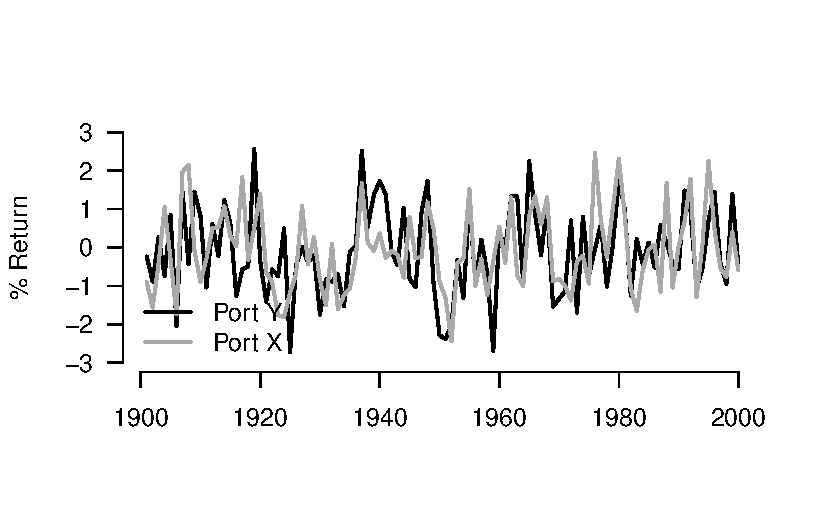
\includegraphics{./03-DescriptiveII_files/figure-pdf/unnamed-chunk-14-1.pdf}

}

\end{figure}

\hypertarget{descriptive-statistics-iii}{%
\chapter{Descriptive Statistics III}\label{descriptive-statistics-iii}}

\hypertarget{concepts-2}{%
\section{Concepts}\label{concepts-2}}

\hypertarget{measures-of-central-location}{%
\subsection*{Measures of Central
Location}\label{measures-of-central-location}}
\addcontentsline{toc}{subsection}{Measures of Central Location}

Measures of Central Location determine where the center of a
distribution lies.

\begin{itemize}
\item
  The \textbf{mean} is the average value for a numerical variable. The
  sample statistic is estimated by \(\bar{x}=\sum x_{i}/n\), where
  \(x_i\) is observation \(i\), and \(n\) is the number of observations.
  The population parameter is defined as \(\mu=\sum x_{i}/N\).
\item
  The \textbf{median} is the value in the middle when data is organized
  in ascending order. When \(n\) is even, the median is the average
  between the two middle values.
\item
  The \textbf{mode} is the value with highest frequency from a set of
  observations.
\item
  The \textbf{weighted mean} uses weights to determine the importance of
  each data point of a variable. It is calculated by
  \(\frac{\sum w_{i}x_{i}}{\sum w_{i}}\), where \(w_{i}\) are the
  weights associated to the values \(x_{i}\).
\item
  The \textbf{geometric mean} is a multiplicative average that is less
  sensitive to outliers. It is used to average growth rates or rated of
  return. It is calculated by \(\sqrt[n]{(1+r_1)*(1+r_2)...(1+r_n)}-1\),
  where \(\sqrt[n]{}\) is the \(n_{th}\) root, and \(r_i\) are the
  returns or growth rates.
\end{itemize}

\hypertarget{useful-r-functions-2}{%
\subsection*{Useful R functions}\label{useful-r-functions-2}}
\addcontentsline{toc}{subsection}{Useful R functions}

Base R has a collection of functions that calculate measures of central
location.

\begin{itemize}
\item
  The \texttt{mean()} function calculates the average of a vector of
  values.
\item
  The \texttt{median()} function returns the median of a vector of
  values.
\item
  The \texttt{table()} function provides us with a frequency
  distribution. We can then identify the mode(s) of the vector provided.
\item
  The \texttt{summary()} function returns a collection of descriptive
  statistics for a vector or data frame.
\end{itemize}

\hypertarget{exercises-2}{%
\section{Exercises}\label{exercises-2}}

The following exercises will help you practice the measures of central
location. In particular, the exercises work on:

\begin{itemize}
\item
  Calculating the mean, median, and the mode.
\item
  Calculating the weighted average.
\item
  Applying the geometric mean for growth rates and returns.
\end{itemize}

Answers are provided below. Try not to peak until you have a formulated
your own answer and double checked your work for any mistakes.

\hypertarget{exercise-1-4}{%
\subsection*{Exercise 1}\label{exercise-1-4}}
\addcontentsline{toc}{subsection}{Exercise 1}

For the following exercises, make your calculations by hand and verify
results using R functions when possible.

\begin{enumerate}
\def\labelenumi{\arabic{enumi}.}
\item
  Use the following observations to calculate the mean, the median, and
  the mode.

  \begin{longtable}[]{@{}ccccc@{}}
  \toprule()
  \endhead
  8 & 10 & 9 & 12 & 12 \\
  \bottomrule()
  \end{longtable}
\item
  Use following observations to calculate the mean, the median, and the
  mode.

  \begin{longtable}[]{@{}cccccc@{}}
  \toprule()
  \endhead
  -4 & 0 & -6 & 1 & -3 & -4 \\
  \bottomrule()
  \end{longtable}
\item
  Use the following observations, calculate the mean, the median, and
  the mode.

  \begin{longtable}[]{@{}ccccccccc@{}}
  \toprule()
  \endhead
  20 & 15 & 25 & 20 & 10 & 15 & 25 & 20 & 15 \\
  \bottomrule()
  \end{longtable}
\end{enumerate}

\hypertarget{exercise-2-4}{%
\subsection*{Exercise 2}\label{exercise-2-4}}
\addcontentsline{toc}{subsection}{Exercise 2}

Download the \texttt{ISLR2} package. You will need the \textbf{OJ} data
set to answer this question.

\begin{enumerate}
\def\labelenumi{\arabic{enumi}.}
\item
  Find the mean price for Country Hill (\emph{PriceCH}) and Minute Maid
  (\emph{PriceMM}).
\item
  Find the mean price of Country Hill (\emph{PriceCH}) in store 1 and
  store 2 (\emph{StoreID}). Which store had the better price?
\item
  Find the mean price paid by Country Hill (\emph{PriceCH}) purchasers
  (\emph{Purchase}) in store 1 (\emph{StoreID})? How about store 2?
  Which store had the better price?
\end{enumerate}

\hypertarget{exercise-3-4}{%
\subsection*{Exercise 3}\label{exercise-3-4}}
\addcontentsline{toc}{subsection}{Exercise 3}

\begin{enumerate}
\def\labelenumi{\arabic{enumi}.}
\tightlist
\item
  Over the past year an investor bought TSLA. She made these purchases
  on three occasions at the prices shown in the table below. Calculate
  the average price per share.
\end{enumerate}

\begin{longtable}[]{@{}ccc@{}}
\toprule()
Date & Price Per Share & Number of Shares \\
\midrule()
\endhead
February & 250.34 & 80 \\
April & 234.59 & 120 \\
Aug & 270.45 & 50 \\
\bottomrule()
\end{longtable}

\begin{enumerate}
\def\labelenumi{\arabic{enumi}.}
\setcounter{enumi}{1}
\tightlist
\item
  What would have been the average price per share if the investor would
  have bought equal amounts of shares each month?
\end{enumerate}

\hypertarget{exercise-4}{%
\subsection*{Exercise 4}\label{exercise-4}}
\addcontentsline{toc}{subsection}{Exercise 4}

\begin{enumerate}
\def\labelenumi{\arabic{enumi}.}
\item
  Consider the following observations for the consumer price index
  (CPI). Calculate the inflation rate (Growth Rate of the CPI) for each
  period.

  \begin{longtable}[]{@{}ccccc@{}}
  \toprule()
  \endhead
  1.0 & 1.3 & 1.6 & 1.8 & 2.1 \\
  \bottomrule()
  \end{longtable}
\item
  Suppose that you want to invest \$1000 dollars in a stock that is
  predicted to yield the following returns in the next four years.
  Calculate both the arithmetic mean and the geometric mean. Use the
  geometric mean to estimate how much money you would have by the end of
  year 4.

  \begin{longtable}[]{@{}cc@{}}
  \toprule()
  Year & Annual Return \\
  \midrule()
  \endhead
  1 & 17.3 \\
  2 & 19.6 \\
  3 & 6.8 \\
  4 & 8.2 \\
  \bottomrule()
  \end{longtable}
\end{enumerate}

\hypertarget{answers-2}{%
\section{Answers}\label{answers-2}}

\hypertarget{exercise-1-5}{%
\subsection*{Exercise 1}\label{exercise-1-5}}
\addcontentsline{toc}{subsection}{Exercise 1}

\begin{blackbox}

\begin{enumerate}
\def\labelenumi{\arabic{enumi}.}
\item
  To find the mean we will use the following formula
  \(( \frac{1}{n} \sum_{i=i}^{n} x_{i})\). The summation of the values
  is \(51\) and the number of observations is \(5\). The mean is
  \(51/5=10.2\).

  The median is found by locating the middle value when data is sorted
  in ascending order. The median in this example is \(10\).

  The mode is the value with the highest frequency. In this example the
  mode is \(12\) since it is repeated twice and all other numbers appear
  only once.
\end{enumerate}

\end{blackbox}

The mean can be easily verified in R by using the \texttt{mean()}
function:

\begin{Shaded}
\begin{Highlighting}[numbers=left,,]
\FunctionTok{mean}\NormalTok{(}\FunctionTok{c}\NormalTok{(}\DecValTok{8}\NormalTok{,}\DecValTok{10}\NormalTok{,}\DecValTok{9}\NormalTok{,}\DecValTok{12}\NormalTok{,}\DecValTok{12}\NormalTok{))}
\end{Highlighting}
\end{Shaded}

\begin{verbatim}
[1] 10.2
\end{verbatim}

Similarly, the median is easily verified by using the \texttt{median()}
function:

\begin{Shaded}
\begin{Highlighting}[numbers=left,,]
\FunctionTok{median}\NormalTok{(}\FunctionTok{c}\NormalTok{(}\DecValTok{8}\NormalTok{,}\DecValTok{10}\NormalTok{,}\DecValTok{9}\NormalTok{,}\DecValTok{12}\NormalTok{,}\DecValTok{12}\NormalTok{))}
\end{Highlighting}
\end{Shaded}

\begin{verbatim}
[1] 10
\end{verbatim}

We can use the \texttt{table()} function to calculate frequencies and
easily identify the mode.

\begin{Shaded}
\begin{Highlighting}[numbers=left,,]
\FunctionTok{table}\NormalTok{(}\FunctionTok{c}\NormalTok{(}\DecValTok{8}\NormalTok{,}\DecValTok{10}\NormalTok{,}\DecValTok{9}\NormalTok{,}\DecValTok{12}\NormalTok{,}\DecValTok{12}\NormalTok{))}
\end{Highlighting}
\end{Shaded}

\begin{verbatim}

 8  9 10 12 
 1  1  1  2 
\end{verbatim}

\begin{blackbox}

\begin{enumerate}
\def\labelenumi{\arabic{enumi}.}
\setcounter{enumi}{1}
\tightlist
\item
  The mean is \(-2.67\), the median is \(-3.5\), the mode is \(-4\).
\end{enumerate}

\end{blackbox}

These mean is verified in R:

\begin{Shaded}
\begin{Highlighting}[numbers=left,,]
\FunctionTok{mean}\NormalTok{(}\FunctionTok{c}\NormalTok{(}\SpecialCharTok{{-}}\DecValTok{4}\NormalTok{,}\DecValTok{0}\NormalTok{,}\SpecialCharTok{{-}}\DecValTok{6}\NormalTok{,}\DecValTok{1}\NormalTok{,}\SpecialCharTok{{-}}\DecValTok{3}\NormalTok{,}\SpecialCharTok{{-}}\DecValTok{4}\NormalTok{))}
\end{Highlighting}
\end{Shaded}

\begin{verbatim}
[1] -2.666667
\end{verbatim}

The median in R:

\begin{Shaded}
\begin{Highlighting}[numbers=left,,]
\FunctionTok{median}\NormalTok{(}\FunctionTok{c}\NormalTok{(}\SpecialCharTok{{-}}\DecValTok{4}\NormalTok{,}\DecValTok{0}\NormalTok{,}\SpecialCharTok{{-}}\DecValTok{6}\NormalTok{,}\DecValTok{1}\NormalTok{,}\SpecialCharTok{{-}}\DecValTok{3}\NormalTok{,}\SpecialCharTok{{-}}\DecValTok{4}\NormalTok{))}
\end{Highlighting}
\end{Shaded}

\begin{verbatim}
[1] -3.5
\end{verbatim}

Finally, the mode in R:

\begin{Shaded}
\begin{Highlighting}[numbers=left,,]
\FunctionTok{table}\NormalTok{(}\FunctionTok{c}\NormalTok{(}\SpecialCharTok{{-}}\DecValTok{4}\NormalTok{,}\DecValTok{0}\NormalTok{,}\SpecialCharTok{{-}}\DecValTok{6}\NormalTok{,}\DecValTok{1}\NormalTok{,}\SpecialCharTok{{-}}\DecValTok{3}\NormalTok{,}\SpecialCharTok{{-}}\DecValTok{4}\NormalTok{))}
\end{Highlighting}
\end{Shaded}

\begin{verbatim}

-6 -4 -3  0  1 
 1  2  1  1  1 
\end{verbatim}

\begin{blackbox}

\begin{enumerate}
\def\labelenumi{\arabic{enumi}.}
\setcounter{enumi}{2}
\tightlist
\item
  The mean is \(18.33\), the median is \(20\), the data is bimodal with
  both \(15\) and \(20\) being modes.
\end{enumerate}

\end{blackbox}

These mean is verified in R:

\begin{Shaded}
\begin{Highlighting}[numbers=left,,]
\FunctionTok{mean}\NormalTok{(}\FunctionTok{c}\NormalTok{(}\DecValTok{20}\NormalTok{,}\DecValTok{15}\NormalTok{,}\DecValTok{25}\NormalTok{,}\DecValTok{20}\NormalTok{,}\DecValTok{10}\NormalTok{,}\DecValTok{15}\NormalTok{,}\DecValTok{25}\NormalTok{,}\DecValTok{20}\NormalTok{,}\DecValTok{15}\NormalTok{))}
\end{Highlighting}
\end{Shaded}

\begin{verbatim}
[1] 18.33333
\end{verbatim}

The median in R:

\begin{Shaded}
\begin{Highlighting}[numbers=left,,]
\FunctionTok{median}\NormalTok{(}\FunctionTok{c}\NormalTok{(}\DecValTok{20}\NormalTok{,}\DecValTok{15}\NormalTok{,}\DecValTok{25}\NormalTok{,}\DecValTok{20}\NormalTok{,}\DecValTok{10}\NormalTok{,}\DecValTok{15}\NormalTok{,}\DecValTok{25}\NormalTok{,}\DecValTok{20}\NormalTok{,}\DecValTok{15}\NormalTok{))}
\end{Highlighting}
\end{Shaded}

\begin{verbatim}
[1] 20
\end{verbatim}

The frequency distribution identifies the modes:

\begin{Shaded}
\begin{Highlighting}[numbers=left,,]
\FunctionTok{table}\NormalTok{(}\FunctionTok{c}\NormalTok{(}\DecValTok{20}\NormalTok{,}\DecValTok{15}\NormalTok{,}\DecValTok{25}\NormalTok{,}\DecValTok{20}\NormalTok{,}\DecValTok{10}\NormalTok{,}\DecValTok{15}\NormalTok{,}\DecValTok{25}\NormalTok{,}\DecValTok{20}\NormalTok{,}\DecValTok{15}\NormalTok{))}
\end{Highlighting}
\end{Shaded}

\begin{verbatim}

10 15 20 25 
 1  3  3  2 
\end{verbatim}

\hypertarget{exercise-2-5}{%
\subsection*{Exercise 2}\label{exercise-2-5}}
\addcontentsline{toc}{subsection}{Exercise 2}

\begin{blackbox}

\begin{enumerate}
\def\labelenumi{\arabic{enumi}.}
\tightlist
\item
  The mean price for Country Hill is \(1.87\). The mean price for Minute
  Maid is \(2.09\).
\end{enumerate}

\end{blackbox}

The means can be easily found with the \texttt{mean()} function:

\begin{Shaded}
\begin{Highlighting}[numbers=left,,]
\FunctionTok{library}\NormalTok{(ISLR2)}
\FunctionTok{mean}\NormalTok{(OJ}\SpecialCharTok{$}\NormalTok{PriceCH)}
\end{Highlighting}
\end{Shaded}

\begin{verbatim}
[1] 1.867421
\end{verbatim}

\begin{Shaded}
\begin{Highlighting}[numbers=left,,]
\FunctionTok{mean}\NormalTok{(OJ}\SpecialCharTok{$}\NormalTok{PriceMM)}
\end{Highlighting}
\end{Shaded}

\begin{verbatim}
[1] 2.085411
\end{verbatim}

\begin{blackbox}

\begin{enumerate}
\def\labelenumi{\arabic{enumi}.}
\setcounter{enumi}{1}
\tightlist
\item
  The mean price at store 1 for Country Hill is \(1.80\) vs.~\(1.84\)
  for store 2. The juice is cheaper at store 1.
\end{enumerate}

\end{blackbox}

The means for each store can be found by using indexing and a logical
statement. The Country Hill mean price at store 1 is given by:

\begin{Shaded}
\begin{Highlighting}[numbers=left,,]
\FunctionTok{mean}\NormalTok{(OJ}\SpecialCharTok{$}\NormalTok{PriceCH[OJ}\SpecialCharTok{$}\NormalTok{StoreID}\SpecialCharTok{==}\DecValTok{1}\NormalTok{])}
\end{Highlighting}
\end{Shaded}

\begin{verbatim}
[1] 1.803758
\end{verbatim}

The Country Hill mean price at store 2 is given by:

\begin{Shaded}
\begin{Highlighting}[numbers=left,,]
\FunctionTok{mean}\NormalTok{(OJ}\SpecialCharTok{$}\NormalTok{PriceCH[OJ}\SpecialCharTok{$}\NormalTok{StoreID}\SpecialCharTok{==}\DecValTok{2}\NormalTok{])}
\end{Highlighting}
\end{Shaded}

\begin{verbatim}
[1] 1.841216
\end{verbatim}

\begin{blackbox}

\begin{enumerate}
\def\labelenumi{\arabic{enumi}.}
\setcounter{enumi}{2}
\tightlist
\item
  Purchasers of Country Hill at store 1 paid and average of \(1.80\) for
  Country Hill juice. At store 2 they paid \(1.86\). Once again the
  average price was lower at store 1.
\end{enumerate}

\end{blackbox}

The mean for Country Hill purchasers at store 1 is given by:

\begin{Shaded}
\begin{Highlighting}[numbers=left,,]
\FunctionTok{mean}\NormalTok{(OJ}\SpecialCharTok{$}\NormalTok{PriceCH[OJ}\SpecialCharTok{$}\NormalTok{StoreID}\SpecialCharTok{==}\DecValTok{1} \SpecialCharTok{\&}\NormalTok{ OJ}\SpecialCharTok{$}\NormalTok{Purchase}\SpecialCharTok{==}\StringTok{"CH"}\NormalTok{])}
\end{Highlighting}
\end{Shaded}

\begin{verbatim}
[1] 1.797176
\end{verbatim}

The mean for Country Hill purchasers at store 2 is:

\begin{Shaded}
\begin{Highlighting}[numbers=left,,]
\FunctionTok{mean}\NormalTok{(OJ}\SpecialCharTok{$}\NormalTok{PriceCH[OJ}\SpecialCharTok{$}\NormalTok{StoreID}\SpecialCharTok{==}\DecValTok{2} \SpecialCharTok{\&}\NormalTok{ OJ}\SpecialCharTok{$}\NormalTok{Purchase}\SpecialCharTok{==}\StringTok{"CH"}\NormalTok{])}
\end{Highlighting}
\end{Shaded}

\begin{verbatim}
[1] 1.857383
\end{verbatim}

\hypertarget{exercise-3-5}{%
\subsection*{Exercise 3}\label{exercise-3-5}}
\addcontentsline{toc}{subsection}{Exercise 3}

\begin{blackbox}

\begin{enumerate}
\def\labelenumi{\arabic{enumi}.}
\tightlist
\item
  The average price of sale is found by using the weighted average
  formula. \(\frac{\sum w_{i}x_{i}}{\sum w_{i}}\) The weights
  (\(w_{i}\)) are given by the number of shares bought and the values
  (\(x_{i}\)) are the prices. The weighted average is \(246.802\).
\end{enumerate}

\end{blackbox}

In R you can create two vectors. One holds the share price and the other
one the number of shares bought.

\begin{Shaded}
\begin{Highlighting}[numbers=left,,]
\NormalTok{PricePerShare}\OtherTok{\textless{}{-}}\FunctionTok{c}\NormalTok{(}\FloatTok{250.34}\NormalTok{,}\FloatTok{234.59}\NormalTok{,}\FloatTok{270.45}\NormalTok{)}
\NormalTok{NumberOfShares}\OtherTok{\textless{}{-}}\FunctionTok{c}\NormalTok{(}\DecValTok{80}\NormalTok{,}\DecValTok{120}\NormalTok{,}\DecValTok{50}\NormalTok{)}
\end{Highlighting}
\end{Shaded}

Next, you can multiply the \emph{PricePerShare} and
\emph{NumberOfShares} vectors to find the numerator and then use
\texttt{sum()} function to find the denominator. The weighted average
is:

\begin{Shaded}
\begin{Highlighting}[numbers=left,,]
\NormalTok{(WeightedAverage}\OtherTok{\textless{}{-}}
  \FunctionTok{sum}\NormalTok{(PricePerShare}\SpecialCharTok{*}\NormalTok{NumberOfShares)}\SpecialCharTok{/}\FunctionTok{sum}\NormalTok{(NumberOfShares))}
\end{Highlighting}
\end{Shaded}

\begin{verbatim}
[1] 246.802
\end{verbatim}

\begin{blackbox}

\begin{enumerate}
\def\labelenumi{\arabic{enumi}.}
\setcounter{enumi}{1}
\tightlist
\item
  The average if equal shares were bought would be \(251.7933\).
\end{enumerate}

\end{blackbox}

In R you can use the \texttt{mean()} function on the PricePerShare
vector.

\begin{Shaded}
\begin{Highlighting}[numbers=left,,]
\NormalTok{(Average}\OtherTok{\textless{}{-}}\FunctionTok{mean}\NormalTok{(PricePerShare))}
\end{Highlighting}
\end{Shaded}

\begin{verbatim}
[1] 251.7933
\end{verbatim}

\hypertarget{exercise-4-1}{%
\subsection*{Exercise 4}\label{exercise-4-1}}
\addcontentsline{toc}{subsection}{Exercise 4}

\begin{blackbox}

\begin{enumerate}
\def\labelenumi{\arabic{enumi}.}
\tightlist
\item
  The inflation rate for each period is shown in the table below:
\end{enumerate}

\begin{longtable}[]{@{}cccc@{}}
\toprule()
\endhead
30\% & 23.08\% & 12.5\% & 16.67\% \\
\bottomrule()
\end{longtable}

\end{blackbox}

In R create an object to store the values of the CPI:

\begin{Shaded}
\begin{Highlighting}[numbers=left,,]
\NormalTok{CPI}\OtherTok{\textless{}{-}}\FunctionTok{c}\NormalTok{(}\DecValTok{1}\NormalTok{,}\FloatTok{1.3}\NormalTok{,}\FloatTok{1.6}\NormalTok{,}\FloatTok{1.8}\NormalTok{,}\FloatTok{2.1}\NormalTok{)}
\end{Highlighting}
\end{Shaded}

Next use the \texttt{diff()} function to find the difference between the
end value and start value. Divide the result by a vector of starting
value and multiply times 100.

\begin{Shaded}
\begin{Highlighting}[numbers=left,,]
\NormalTok{(Inflation}\OtherTok{\textless{}{-}}\DecValTok{100}\SpecialCharTok{*}\FunctionTok{diff}\NormalTok{(CPI)}\SpecialCharTok{/}\NormalTok{CPI[}\DecValTok{1}\SpecialCharTok{:}\DecValTok{4}\NormalTok{])}
\end{Highlighting}
\end{Shaded}

\begin{verbatim}
[1] 30.00000 23.07692 12.50000 16.66667
\end{verbatim}

\begin{blackbox}

\begin{enumerate}
\def\labelenumi{\arabic{enumi}.}
\setcounter{enumi}{1}
\tightlist
\item
  At the end of 4 years it is predicted that you would have \(1621.17\)
  dollars. Each year you would have gained \(12.84\)\% on average.
\end{enumerate}

\end{blackbox}

In R include the annual rates in a vector:

\begin{Shaded}
\begin{Highlighting}[numbers=left,,]
\NormalTok{growth}\OtherTok{\textless{}{-}}\FunctionTok{c}\NormalTok{(}\FloatTok{0.173}\NormalTok{,}\FloatTok{0.196}\NormalTok{,}\FloatTok{0.068}\NormalTok{,}\FloatTok{0.082}\NormalTok{)}
\end{Highlighting}
\end{Shaded}

The arithmetic mean is:

\begin{Shaded}
\begin{Highlighting}[numbers=left,,]
\DecValTok{100}\SpecialCharTok{*}\FunctionTok{mean}\NormalTok{(growth)}
\end{Highlighting}
\end{Shaded}

\begin{verbatim}
[1] 12.975
\end{verbatim}

The geometric mean is:

\begin{Shaded}
\begin{Highlighting}[numbers=left,,]
\NormalTok{(geom}\OtherTok{\textless{}{-}}\NormalTok{((}\FunctionTok{prod}\NormalTok{(}\DecValTok{1}\SpecialCharTok{+}\NormalTok{growth))}\SpecialCharTok{\^{}}\NormalTok{(}\DecValTok{1}\SpecialCharTok{/}\DecValTok{4}\NormalTok{)}\SpecialCharTok{{-}}\DecValTok{1}\NormalTok{)}\SpecialCharTok{*}\DecValTok{100}\NormalTok{)}
\end{Highlighting}
\end{Shaded}

\begin{verbatim}
[1] 12.8384
\end{verbatim}

At the end of the four years we would have:

\begin{Shaded}
\begin{Highlighting}[numbers=left,,]
\DecValTok{1000}\SpecialCharTok{*}\NormalTok{(}\DecValTok{1}\SpecialCharTok{+}\NormalTok{geom}\SpecialCharTok{/}\DecValTok{100}\NormalTok{)}\SpecialCharTok{\^{}}\DecValTok{4}
\end{Highlighting}
\end{Shaded}

\begin{verbatim}
[1] 1621.167
\end{verbatim}

\hypertarget{descriptive-stats-iv}{%
\chapter{Descriptive Stats IV}\label{descriptive-stats-iv}}

\hypertarget{concepts-3}{%
\section{Concepts}\label{concepts-3}}

\hypertarget{measures-of-dispersion}{%
\subsection*{Measures of Dispersion}\label{measures-of-dispersion}}
\addcontentsline{toc}{subsection}{Measures of Dispersion}

Measures of dispersion are used to determine the spread (variability) of
the data.

\begin{itemize}
\item
  The \textbf{range} is calculated by \(largest-smallest\). It ignores
  the variability of the data between the largest and smallest values.
\item
  The \textbf{variance} calculates the dispersion around the mean. It
  uses squared deviations. The population parameter is given by
  \(\sigma^2= \frac{\sum (x_i-\mu)^2}{N}\), while the sample statistic
  is \(s^2=\frac{\sum (x_i-\bar{x})^2}{n-1}\).
\item
  The \textbf{standard deviation} measures the average deviation around
  the mean. It is calculated as the square root of the variance. For the
  population parameter use \(\sigma=\sqrt{\sigma^2}\) and
  \(s=\sqrt{s^2}\) for the sample statistic.
\item
  The \textbf{Mean Absolute Deviation} (\(MAD\)) measures the average
  deviation from the mean. This measure uses absolute deviations. It is
  calculated by \(MAD=\frac{\sum |x_i-\mu|}{N}\) for the population and
  \(mad=\frac{\sum |x_i-\bar{x}|}{n}\) for the sample.
\item
  The \textbf{coefficient of variation} \(CV=s/\bar{x}\) adjusts the
  standard deviation for differences in units of measure or scale.
\end{itemize}

\hypertarget{portfolio-assesment}{%
\subsection*{Portfolio Assesment}\label{portfolio-assesment}}
\addcontentsline{toc}{subsection}{Portfolio Assesment}

To asses the performance of a portfolio calculate:

\begin{itemize}
\item
  The mean return of the portfolio
  \(\alpha\bar{R}_1+(1-\alpha)\bar{R}_2\), where \(\alpha\) is the
  weight of investment 1 in the portfolio and \(\bar{R}_i\) is the
  average return of investment \(i \in\)\{\(1\),\(2\)\}.
\item
  The variance of the portfolio is given by
  \(\begin{bmatrix} \alpha \\ 1-\alpha \end{bmatrix}^T \begin{bmatrix} s_x^2 & s_{xy} \\ s_{xy} & s_y^2 \end{bmatrix} \begin{bmatrix} \alpha \\ 1-\alpha \end{bmatrix}\)
\item
  The \textbf{Sharpe ratio} quantifies the excess return of an
  investment over the risk free return. It is calculated by
  \(\frac{\bar{R_p}-R_f}{s}\), where \(\bar{R_p}\) is the mean return of
  the portfolio, \(R_f\) is the risk free return, and \(s\) is the
  standard deviation.
\end{itemize}

\hypertarget{useful-r-functions-3}{%
\subsection*{Useful R Functions}\label{useful-r-functions-3}}
\addcontentsline{toc}{subsection}{Useful R Functions}

The \texttt{range()} function returns the maximum and minimum of a
vector of values.

The \texttt{diff()} function finds the first difference of a vector.

The \texttt{var()} function calculates the sample variance for a vector
of values. To calculate the population variance, adjust the result by a
factor of \((n-1)/n\).

The \texttt{sd()} function calculates the sample standard deviation.

The \texttt{matrix()} function defines a matrix.

When dealing with matrices, the \texttt{t()} function transposes a
vector or matrix, and the operator \texttt{\%*\%} performs matrix
multiplication.

\hypertarget{exercises-3}{%
\section{Exercises}\label{exercises-3}}

The following exercises will help you practice the measures of
dispersion. In particular, the exercises work on:

\begin{itemize}
\item
  Calculating the range, MAD, variance, and the standard deviation.
\item
  Using R to calculate measures of dispersion.
\item
  Calculating and using the Sharpe ratio to select investments.
\end{itemize}

Answers are provided below. Try not to peak until you have a formulated
your own answer and double checked your work for any mistakes.

\hypertarget{exercise-1-6}{%
\subsection*{Exercise 1}\label{exercise-1-6}}
\addcontentsline{toc}{subsection}{Exercise 1}

For the following exercises, make your calculations by hand and verify
results using R functions when possible. Make sure to calculate the
deviations from the mean.

\begin{enumerate}
\def\labelenumi{\arabic{enumi}.}
\item
  Use the following observations to calculate the Range, MAD, Variance
  and Standard Deviation. Assume that the data below is the entire
  population.

  \begin{longtable}[]{@{}cccc@{}}
  \toprule()
  \endhead
  70 & 68 & 4 & 98 \\
  \bottomrule()
  \end{longtable}
\item
  Use the following observations to calculate the Range, MAD, Variance
  and Standard Deviation. Assume that the data below is a sample from
  the population.

  \begin{longtable}[]{@{}cccccc@{}}
  \toprule()
  \endhead
  -4 & 0 & -6 & 1 & -3 & 0 \\
  \bottomrule()
  \end{longtable}
\end{enumerate}

\hypertarget{exercise-2-6}{%
\subsection*{Exercise 2}\label{exercise-2-6}}
\addcontentsline{toc}{subsection}{Exercise 2}

You will need the \textbf{Stocks} data set to answer this question. You
can find this data at https://jagelves.github.io/Data/Stocks.csv The
data is a sample of daily stock prices for ticker symbols TSLA (Tesla),
VTI (S\&P 500) and GBTC (Bitcoin).

\begin{enumerate}
\def\labelenumi{\arabic{enumi}.}
\tightlist
\item
  Calculate the standard deviations for each stock. Which stock had the
  lowest standard deviation?
\item
  Calculate the MAD. Does your answer in 1. remain the same?
\item
  Finally, calculate the coefficient of variation. Any changes to your
  conclusions?
\end{enumerate}

\hypertarget{exercise-3-6}{%
\subsection*{Exercise 3}\label{exercise-3-6}}
\addcontentsline{toc}{subsection}{Exercise 3}

Install the \texttt{ISLR2} package. You will need the \textbf{Portfolio}
data set to answer this question. The data has 100 records of the
returns of two stocks.

\begin{enumerate}
\def\labelenumi{\arabic{enumi}.}
\tightlist
\item
  Calculate the mean and standard deviation for each stock. Which
  investment has higher returns on average? Which investment is safest
  as measured by the standard deviation?
\item
  Use a Risk Free rate of return of 3.5\% to calculate the Sharpe ratio
  for each stock. Which stock would you recommend?
\item
  Calculate the average return for a portfolio that has 30\% of stock X
  and 70\% of stock Y. What is the standard deviation of the portfolio?
\end{enumerate}

\hypertarget{answers-3}{%
\section{Answers}\label{answers-3}}

\hypertarget{exercise-1-7}{%
\subsection*{Exercise 1}\label{exercise-1-7}}
\addcontentsline{toc}{subsection}{Exercise 1}

\begin{blackbox}

\begin{enumerate}
\def\labelenumi{\arabic{enumi}.}
\tightlist
\item
  The mean is \(60\), the Range is \(94\), the MAD is \(28\), the
  variance is \(1186\) and the variance is \(34.44\).
\end{enumerate}

\end{blackbox}

Start by crating a vector to hold the values:

\begin{Shaded}
\begin{Highlighting}[numbers=left,,]
\NormalTok{Ex1}\OtherTok{\textless{}{-}}\FunctionTok{c}\NormalTok{(}\DecValTok{70}\NormalTok{,}\DecValTok{68}\NormalTok{,}\DecValTok{4}\NormalTok{,}\DecValTok{98}\NormalTok{)}
\end{Highlighting}
\end{Shaded}

The range can be calculated by using the \texttt{range()} and
\texttt{diff()} functions in R.

\begin{Shaded}
\begin{Highlighting}[numbers=left,,]
\NormalTok{(Range}\OtherTok{\textless{}{-}}\FunctionTok{diff}\NormalTok{(}\FunctionTok{range}\NormalTok{(Ex1)))}
\end{Highlighting}
\end{Shaded}

\begin{verbatim}
[1] 94
\end{verbatim}

Next, we can create a table by hand that captures the deviations from
the mean. Let's calculate the mean first:

\begin{Shaded}
\begin{Highlighting}[numbers=left,,]
\NormalTok{(Average1}\OtherTok{\textless{}{-}}\FunctionTok{mean}\NormalTok{(Ex1))}
\end{Highlighting}
\end{Shaded}

\begin{verbatim}
[1] 60
\end{verbatim}

Now we can use the mean to fill out a table of deviations:

\begin{longtable}[]{@{}cccc@{}}
\toprule()
\(x_{i}\) & \(x_{i}-\bar{x}\) & \((x_{i}-\bar{x})^2\) &
\(|x_{i}-\bar{x}|\) \\
\midrule()
\endhead
70 & 10 & 100 & 10 \\
68 & 8 & 64 & 8 \\
4 & -56 & 3136 & 56 \\
98 & 38 & 1444 & 38 \\
\bottomrule()
\end{longtable}

The variance averages out the squared deviations \((x_{i}-\bar{x})^2\),
the MAD averages out the absolute deviations \(|x_{i}-\bar{x}|\), and
the standard deviation is the square root of the variance.

Let's verify the variance in R:

\begin{Shaded}
\begin{Highlighting}[numbers=left,,]
\NormalTok{SquaredDeviations1}\OtherTok{\textless{}{-}}\NormalTok{(Ex1}\SpecialCharTok{{-}}\NormalTok{Average1)}\SpecialCharTok{\^{}}\DecValTok{2}
\NormalTok{AverageDeviations1}\OtherTok{\textless{}{-}}\FunctionTok{mean}\NormalTok{(SquaredDeviations1)}
\FunctionTok{var}\NormalTok{(Ex1)}\SpecialCharTok{*}\DecValTok{3}\SpecialCharTok{/}\DecValTok{4}
\end{Highlighting}
\end{Shaded}

\begin{verbatim}
[1] 1186
\end{verbatim}

Note that R calculates the sample variance. Hence, we must multiply the
result by \(3/4\) to get the population variance. The standard deviation
is just the square root of the variance:

\begin{Shaded}
\begin{Highlighting}[numbers=left,,]
\FunctionTok{sqrt}\NormalTok{(AverageDeviations1)}
\end{Highlighting}
\end{Shaded}

\begin{verbatim}
[1] 34.43835
\end{verbatim}

Lastly, the MAD is calculated by averaging the absolute deviations
\(|x_{i}-\bar{x}|\).

\begin{Shaded}
\begin{Highlighting}[numbers=left,,]
\NormalTok{AbsoluteDeviations1}\OtherTok{\textless{}{-}}\FunctionTok{abs}\NormalTok{(Ex1}\SpecialCharTok{{-}}\NormalTok{Average1)}
\FunctionTok{mean}\NormalTok{(AbsoluteDeviations1)}
\end{Highlighting}
\end{Shaded}

\begin{verbatim}
[1] 28
\end{verbatim}

\begin{blackbox}

\begin{enumerate}
\def\labelenumi{\arabic{enumi}.}
\setcounter{enumi}{1}
\tightlist
\item
  The mean is \(-2\), Range is \(7\), the MAD is \(2.33\), the variance
  is \(7.6\) and the standard deviation is \(2.76\).
\end{enumerate}

\end{blackbox}

Here is the table of deviations from the mean:

\begin{longtable}[]{@{}cccc@{}}
\toprule()
\(x_{i}\) & \(x_{i}-\bar{x}\) & \((x_{i}-\bar{x})^2\) &
\(|x_{i}-\bar{x}|\) \\
\midrule()
\endhead
-4 & -2 & 4 & 2 \\
0 & 2 & 4 & 2 \\
-6 & -4 & 16 & 4 \\
1 & 3 & 9 & 3 \\
-3 & -1 & 1 & 1 \\
0 & 2 & 4 & 2 \\
\bottomrule()
\end{longtable}

We can check the results in R. Let's start with the variance:

\begin{Shaded}
\begin{Highlighting}[numbers=left,,]
\NormalTok{Ex2}\OtherTok{\textless{}{-}}\FunctionTok{c}\NormalTok{(}\SpecialCharTok{{-}}\DecValTok{4}\NormalTok{,}\DecValTok{0}\NormalTok{,}\SpecialCharTok{{-}}\DecValTok{6}\NormalTok{,}\DecValTok{1}\NormalTok{,}\SpecialCharTok{{-}}\DecValTok{3}\NormalTok{,}\DecValTok{0}\NormalTok{)}
\FunctionTok{var}\NormalTok{(Ex2)}
\end{Highlighting}
\end{Shaded}

\begin{verbatim}
[1] 7.6
\end{verbatim}

The standard deviation can be found with the \texttt{sd()} function:

\begin{Shaded}
\begin{Highlighting}[numbers=left,,]
\FunctionTok{sd}\NormalTok{(Ex2)}
\end{Highlighting}
\end{Shaded}

\begin{verbatim}
[1] 2.75681
\end{verbatim}

The MAD is given by:

\begin{Shaded}
\begin{Highlighting}[numbers=left,,]
\NormalTok{(MAD}\OtherTok{\textless{}{-}}\FunctionTok{mean}\NormalTok{(}\FunctionTok{abs}\NormalTok{(Ex2}\SpecialCharTok{{-}}\FunctionTok{mean}\NormalTok{(Ex2))))}
\end{Highlighting}
\end{Shaded}

\begin{verbatim}
[1] 2.333333
\end{verbatim}

Lastly, the range:

\begin{Shaded}
\begin{Highlighting}[numbers=left,,]
\FunctionTok{diff}\NormalTok{(}\FunctionTok{range}\NormalTok{(Ex2))}
\end{Highlighting}
\end{Shaded}

\begin{verbatim}
[1] 7
\end{verbatim}

\hypertarget{exercise-2-7}{%
\subsection*{Exercise 2}\label{exercise-2-7}}
\addcontentsline{toc}{subsection}{Exercise 2}

\begin{blackbox}

\begin{enumerate}
\def\labelenumi{\arabic{enumi}.}
\tightlist
\item
  For the sample taken, GBTC has the less variation. The standard
  deviation of GBTC is \(9.43\), which is less than \(16.57\) for VTI or
  \(50.38\) for TSLA.
\end{enumerate}

\end{blackbox}

Start by loading the data set from the website. Since the file is in csv
format, we will use the \texttt{read.csv()} function.

\begin{Shaded}
\begin{Highlighting}[numbers=left,,]
\NormalTok{StockPrices}\OtherTok{\textless{}{-}}\FunctionTok{read.csv}\NormalTok{(}\StringTok{"https://jagelves.github.io/Data/Stocks.csv"}\NormalTok{)}
\end{Highlighting}
\end{Shaded}

Let's start with the standard deviation of the Tesla stock. The standard
deviation is given by:

\begin{Shaded}
\begin{Highlighting}[numbers=left,,]
\FunctionTok{sd}\NormalTok{(StockPrices}\SpecialCharTok{$}\NormalTok{TSLA)}
\end{Highlighting}
\end{Shaded}

\begin{verbatim}
[1] 50.38092
\end{verbatim}

Next, let's find the standard deviation for the S\&P 500 or VTI. The
standard deviation is given by:

\begin{Shaded}
\begin{Highlighting}[numbers=left,,]
\FunctionTok{sd}\NormalTok{(StockPrices}\SpecialCharTok{$}\NormalTok{VTI)}
\end{Highlighting}
\end{Shaded}

\begin{verbatim}
[1] 16.5731
\end{verbatim}

Finally, let's calculate the standard deviation for GBTC or Bitcoin.

\begin{Shaded}
\begin{Highlighting}[numbers=left,,]
\FunctionTok{sd}\NormalTok{(StockPrices}\SpecialCharTok{$}\NormalTok{GBTC)}
\end{Highlighting}
\end{Shaded}

\begin{verbatim}
[1] 9.434213
\end{verbatim}

\begin{blackbox}

\begin{enumerate}
\def\labelenumi{\arabic{enumi}.}
\setcounter{enumi}{1}
\tightlist
\item
  The answer is the same, since the MAD for GBTC is \(8.46\) which is
  lower than \(14.27\) for VTI or \(41.67\) for TSLA.
\end{enumerate}

\end{blackbox}

To calculate the MAD for TSLA we can use the following command:

\begin{Shaded}
\begin{Highlighting}[numbers=left,,]
\NormalTok{(MADTSLA}\OtherTok{\textless{}{-}}\FunctionTok{mean}\NormalTok{(}\FunctionTok{abs}\NormalTok{(StockPrices}\SpecialCharTok{$}\NormalTok{TSLA}\SpecialCharTok{{-}}\FunctionTok{mean}\NormalTok{(StockPrices}\SpecialCharTok{$}\NormalTok{TSLA))))}
\end{Highlighting}
\end{Shaded}

\begin{verbatim}
[1] 41.67163
\end{verbatim}

The MAD for VTI is:

\begin{Shaded}
\begin{Highlighting}[numbers=left,,]
\NormalTok{(MADVTI}\OtherTok{\textless{}{-}}\FunctionTok{mean}\NormalTok{(}\FunctionTok{abs}\NormalTok{(StockPrices}\SpecialCharTok{$}\NormalTok{VTI}\SpecialCharTok{{-}}\FunctionTok{mean}\NormalTok{(StockPrices}\SpecialCharTok{$}\NormalTok{VTI))))}
\end{Highlighting}
\end{Shaded}

\begin{verbatim}
[1] 14.27169
\end{verbatim}

The MAD for GBTC is:

\begin{Shaded}
\begin{Highlighting}[numbers=left,,]
\NormalTok{(MADGBTC}\OtherTok{\textless{}{-}}\FunctionTok{mean}\NormalTok{(}\FunctionTok{abs}\NormalTok{(StockPrices}\SpecialCharTok{$}\NormalTok{GBTC}\SpecialCharTok{{-}}\FunctionTok{mean}\NormalTok{(StockPrices}\SpecialCharTok{$}\NormalTok{GBTC))))}
\end{Highlighting}
\end{Shaded}

\begin{verbatim}
[1] 8.458029
\end{verbatim}

\begin{blackbox}

\begin{enumerate}
\def\labelenumi{\arabic{enumi}.}
\setcounter{enumi}{2}
\tightlist
\item
  By considering the magnitudes of the stock prices, it seems like VTI
  is the less volatile stock. VTI has a CV of \(0.08\) which is lower
  than \(0.44\) for GBTC or \(0.18\) for TSLA. In fact, by CV Bitcoin
  seems to be the most risky asset.
\end{enumerate}

\end{blackbox}

The coefficients of variations are as follows. For TSLA the CV is:

\begin{Shaded}
\begin{Highlighting}[numbers=left,,]
\NormalTok{(CVTSLA}\OtherTok{\textless{}{-}}\FunctionTok{sd}\NormalTok{(StockPrices}\SpecialCharTok{$}\NormalTok{TSLA)}\SpecialCharTok{/}\FunctionTok{mean}\NormalTok{(StockPrices}\SpecialCharTok{$}\NormalTok{TSLA))}
\end{Highlighting}
\end{Shaded}

\begin{verbatim}
[1] 0.1793755
\end{verbatim}

For VTI the CV is:

\begin{Shaded}
\begin{Highlighting}[numbers=left,,]
\NormalTok{(CVVTI}\OtherTok{\textless{}{-}}\FunctionTok{sd}\NormalTok{(StockPrices}\SpecialCharTok{$}\NormalTok{VTI)}\SpecialCharTok{/}\FunctionTok{mean}\NormalTok{(StockPrices}\SpecialCharTok{$}\NormalTok{VTI))}
\end{Highlighting}
\end{Shaded}

\begin{verbatim}
[1] 0.07970004
\end{verbatim}

For GBTC we get:

\begin{Shaded}
\begin{Highlighting}[numbers=left,,]
\NormalTok{(CVGBTC}\OtherTok{\textless{}{-}}\FunctionTok{sd}\NormalTok{(StockPrices}\SpecialCharTok{$}\NormalTok{GBTC)}\SpecialCharTok{/}\FunctionTok{mean}\NormalTok{(StockPrices}\SpecialCharTok{$}\NormalTok{GBTC))}
\end{Highlighting}
\end{Shaded}

\begin{verbatim}
[1] 0.4442497
\end{verbatim}

\hypertarget{exercise-3-7}{%
\subsection*{Exercise 3}\label{exercise-3-7}}
\addcontentsline{toc}{subsection}{Exercise 3}

\begin{blackbox}

\begin{enumerate}
\def\labelenumi{\arabic{enumi}.}
\tightlist
\item
  The best performing stock on average is stock X. It has an average
  return of \(-0.078\)\% vs.~\(0.097\)\% for stock Y. The safest stock
  is stock X as well, since the standard deviation is \(1.062\)
  percentage points vs.~\(1.14\) percentage points for stock Y.
\end{enumerate}

\end{blackbox}

Start by loading the \texttt{ISLR2} package:

\begin{Shaded}
\begin{Highlighting}[numbers=left,,]
\FunctionTok{library}\NormalTok{(ISLR2)}
\end{Highlighting}
\end{Shaded}

Next, calculate the mean for stock X:

\begin{Shaded}
\begin{Highlighting}[numbers=left,,]
\FunctionTok{mean}\NormalTok{(Portfolio}\SpecialCharTok{$}\NormalTok{X)}
\end{Highlighting}
\end{Shaded}

\begin{verbatim}
[1] -0.07713211
\end{verbatim}

and stock Y.

\begin{Shaded}
\begin{Highlighting}[numbers=left,,]
\FunctionTok{mean}\NormalTok{(Portfolio}\SpecialCharTok{$}\NormalTok{Y)}
\end{Highlighting}
\end{Shaded}

\begin{verbatim}
[1] -0.09694472
\end{verbatim}

Then, calculate the standard deviation for stock X

\begin{Shaded}
\begin{Highlighting}[numbers=left,,]
\FunctionTok{sd}\NormalTok{(Portfolio}\SpecialCharTok{$}\NormalTok{X)}
\end{Highlighting}
\end{Shaded}

\begin{verbatim}
[1] 1.062376
\end{verbatim}

and stock Y.

\begin{Shaded}
\begin{Highlighting}[numbers=left,,]
\FunctionTok{sd}\NormalTok{(Portfolio}\SpecialCharTok{$}\NormalTok{Y)}
\end{Highlighting}
\end{Shaded}

\begin{verbatim}
[1] 1.143782
\end{verbatim}

\begin{blackbox}

\begin{enumerate}
\def\labelenumi{\arabic{enumi}.}
\setcounter{enumi}{1}
\tightlist
\item
  The Sharpe Ratio measures the excess return per unit of risk taken.
  Stock X has the better Sharpe Ratio. \(-0.106\) vs.~\(-0.115\). Stock
  X is recommended since it provides a higher excess return per unit of
  risk taken.
\end{enumerate}

\end{blackbox}

To calculate Sharpe Ratios use both the average return, and the standard
deviation. For stock X, the Sharpe Ratio is:

\begin{Shaded}
\begin{Highlighting}[numbers=left,,]
\NormalTok{(}\FunctionTok{mean}\NormalTok{(Portfolio}\SpecialCharTok{$}\NormalTok{X)}\SpecialCharTok{{-}}\FloatTok{0.035}\NormalTok{)}\SpecialCharTok{/}\FunctionTok{sd}\NormalTok{(Portfolio}\SpecialCharTok{$}\NormalTok{X)}
\end{Highlighting}
\end{Shaded}

\begin{verbatim}
[1] -0.1055484
\end{verbatim}

The Sharpe Ratio for stock Y:

\begin{Shaded}
\begin{Highlighting}[numbers=left,,]
\NormalTok{(}\FunctionTok{mean}\NormalTok{(Portfolio}\SpecialCharTok{$}\NormalTok{Y)}\SpecialCharTok{{-}}\FloatTok{0.035}\NormalTok{)}\SpecialCharTok{/}\FunctionTok{sd}\NormalTok{(Portfolio}\SpecialCharTok{$}\NormalTok{Y)}
\end{Highlighting}
\end{Shaded}

\begin{verbatim}
[1] -0.1153583
\end{verbatim}

\begin{blackbox}

\begin{enumerate}
\def\labelenumi{\arabic{enumi}.}
\setcounter{enumi}{2}
\tightlist
\item
  The portfolio has an average return of \(-0.091\) which is worse than
  stock X but better than stock Y. The standard deviation is \(1.00\).
  This is better than stock X and Y separately. The Sharpe ratio of
  \(-0.091\) is also better for the portfolio than for each stock
  individually.
\end{enumerate}

\end{blackbox}

The mean of the portfolio is given by:

\begin{Shaded}
\begin{Highlighting}[numbers=left,,]
\NormalTok{(}\AttributeTok{mean\_return=}\FloatTok{0.3}\SpecialCharTok{*}\FunctionTok{mean}\NormalTok{(Portfolio}\SpecialCharTok{$}\NormalTok{X)}\SpecialCharTok{+}\FloatTok{0.7}\SpecialCharTok{*}\FunctionTok{mean}\NormalTok{(Portfolio}\SpecialCharTok{$}\NormalTok{Y))}
\end{Highlighting}
\end{Shaded}

\begin{verbatim}
[1] -0.09100094
\end{verbatim}

The covariance matrix is given by:

\begin{Shaded}
\begin{Highlighting}[numbers=left,,]
\NormalTok{(risk}\OtherTok{\textless{}{-}}\FunctionTok{cov}\NormalTok{(Portfolio))}
\end{Highlighting}
\end{Shaded}

\begin{verbatim}
          X         Y
X 1.1286424 0.6263583
Y 0.6263583 1.3082375
\end{verbatim}

Using the matrix we can now calculate the standard deviation:

\begin{Shaded}
\begin{Highlighting}[numbers=left,,]
\NormalTok{(standard}\OtherTok{\textless{}{-}}\FunctionTok{sqrt}\NormalTok{(}\FunctionTok{t}\NormalTok{(}\FunctionTok{c}\NormalTok{(}\FloatTok{0.3}\NormalTok{,}\FloatTok{0.7}\NormalTok{)) }\SpecialCharTok{\%*\%}\NormalTok{ (risk }\SpecialCharTok{\%*\%} \FunctionTok{c}\NormalTok{(}\FloatTok{0.3}\NormalTok{,}\FloatTok{0.7}\NormalTok{))))}
\end{Highlighting}
\end{Shaded}

\begin{verbatim}
         [,1]
[1,] 1.002838
\end{verbatim}

Finally, the Sharpe ration for the portfolio is:

\begin{Shaded}
\begin{Highlighting}[numbers=left,,]
\NormalTok{mean\_return}\SpecialCharTok{/}\NormalTok{standard[}\DecValTok{1}\NormalTok{]}
\end{Highlighting}
\end{Shaded}

\begin{verbatim}
[1] -0.09074338
\end{verbatim}

\hypertarget{descriptive-stats-v}{%
\chapter{Descriptive Stats V}\label{descriptive-stats-v}}

\hypertarget{concepts-4}{%
\section{Concepts}\label{concepts-4}}

\hypertarget{quantiles-and-percentiles}{%
\subsection*{Quantiles and
Percentiles}\label{quantiles-and-percentiles}}
\addcontentsline{toc}{subsection}{Quantiles and Percentiles}

A \textbf{quantile} is a location within a set of ranked numbers (or
distribution), below which a certain proportion, \(q\), of that set lie.
Ex: 0.25 of the data lies below the 0.25 quantile.

\textbf{Percentiles} express quantiles in percentage form. Ex: 25\% of
the data lies below the 25th percentile. To calculate a percentile:

\begin{itemize}
\item
  Sort the data in ascending order.
\item
  Compute the location of the percentile desired using
  \(L_{p}=\frac{(n+1)P}{100}\) where \(L_{p}\) is the location of the
  \(P_{th}\) percentile, and \(P\) is the percentile desired.
\item
  The value at \(L_p\), is the the \(P_{th}\) percentile.
\end{itemize}

\hypertarget{chevyshevs-theorem-and-empirical-rule}{%
\subsection*{Chevyshev's Theorem and Empirical
Rule}\label{chevyshevs-theorem-and-empirical-rule}}
\addcontentsline{toc}{subsection}{Chevyshev's Theorem and Empirical
Rule}

\textbf{Chevyshev's Theorem} states that at least \(1-1/z^2\)\% of the
data lies between \(z\) standard deviations from the mean. This result
does not depend on the shape of the distribution.

The \textbf{Empirical Rule} or (\(68\),\(95\),\(99.7\) rule) states that
\(68\)\%, \(95\)\%, and \(99.7\)\% of the data lies between \(1\),
\(2\), and \(3\) standard deviations from the mean respectively. The
rule depends on the data being normally distributed.

\hypertarget{five-point-summary-and-outliers}{%
\subsection*{Five Point Summary and
Outliers}\label{five-point-summary-and-outliers}}
\addcontentsline{toc}{subsection}{Five Point Summary and Outliers}

A popular way to summarize data is by calculating the minimum, first
quartile, median, third quartile and maximum (five point summary).

The \textbf{interquartile range} (IQR) is the difference between the
third quartile and the first quartile.

\textbf{Outliers} are extreme deviations from the mean. They are values
that are not ``normal''. To calculate outliers:

\begin{itemize}
\item
  Use a \textbf{z-score} to measure the distance from the mean in units
  of standard deviation. \(z_{i}=\frac{x_i-\bar{x}}{s_x}\). \(z\)-scores
  above \(3\) are suspected outliers.
\item
  Calculate \(Q_1-1.5(IQR)\) and \(Q_3+1.5(IQR)\), where \(Q_1\) is the
  first quartile, \(Q_3\) is the third quartile, and \(IQR\) is the
  interquartile range. If \(x_i\) is less than \(Q_1-1.5(IQR)\) or
  greater than \(Q_3+1.5(IQR)\), then it is considered an outlier.
\end{itemize}

A \textbf{box plot} is a graph that shows the five point summary,
outliers (if any), and the distribution of data.

To determine if the data is skewed, calculate the \textbf{Pearson's
Coefficient of Skew}. \(Sk=\frac{3(\bar {x}- Median)}{s_x}\). The
distribution is skewed to the left if \(Sk<0\), skewed to the right is
\(Sk>0\), and symmetric if \(Sk=0\).

\hypertarget{useful-r-functions-4}{%
\subsection*{Useful R Functions}\label{useful-r-functions-4}}
\addcontentsline{toc}{subsection}{Useful R Functions}

The \texttt{quantile()} function returns the five point summary when no
arguments are specified. For a specific quantile, specify the
\emph{probs} argument.

The \texttt{boxplot()} command returns a box plot for a vector of
values.

\hypertarget{exercises-4}{%
\section{Exercises}\label{exercises-4}}

The following exercises will help you practice other statistical
measures. In particular, the exercises work on:

\begin{itemize}
\item
  Constructing a five point summary and a boxplot.
\item
  Applying Chebyshev's Theorem.
\item
  Identifying skewness.
\item
  Identifying outliers.
\end{itemize}

Answers are provided below. Try not to peak until you have a formulated
your own answer and double checked your work for any mistakes.

\hypertarget{exercise-1-8}{%
\subsection*{Exercise 1}\label{exercise-1-8}}
\addcontentsline{toc}{subsection}{Exercise 1}

For the following exercises, make your calculations by hand and verify
results using R functions when possible.

\begin{enumerate}
\def\labelenumi{\arabic{enumi}.}
\item
  Use the following observations to calculate the minimum, the first,
  second and third quartiles, and the maximum. Are there any outliers?
  Find the IQR to answer the question.

  \begin{longtable}[]{@{}ccccccc@{}}
  \toprule()
  \endhead
  3 & 10 & 4 & 1 & 0 & 30 & 6 \\
  \bottomrule()
  \end{longtable}
\item
  Confirm your finding of an outlier by calculating the \(z\)-score. Is
  \(30\) an outlier when using a \(z\)-Score?
\item
  Use Chebyshev's theorem to determine what percent of the data falls
  between the \(z\)-score found in \(2\).
\end{enumerate}

\hypertarget{exercise-2-8}{%
\subsection*{Exercise 2}\label{exercise-2-8}}
\addcontentsline{toc}{subsection}{Exercise 2}

You will need the \textbf{Stocks} data set to answer this question. You
can find this data at https://jagelves.github.io/Data/Stocks.csv The
data is a sample of daily stock prices for ticker symbols TSLA (Tesla),
VTI (S\&P 500) and GBTC (Bitcoin).

\begin{enumerate}
\def\labelenumi{\arabic{enumi}.}
\tightlist
\item
  Construct a boxplot for Stock A. Is the data skewed or symmetric?
\item
  Create a histogram of the data. Include a vertical line for the mean
  and median. Explain how the mean and median indicates a skew in the
  data. Calculate the skewness statistic to confirm your result.
\item
  Use a line chart to plot your data. Can you explain why the data has a
  skew?
\end{enumerate}

\hypertarget{exercise-3-8}{%
\subsection*{Exercise 3}\label{exercise-3-8}}
\addcontentsline{toc}{subsection}{Exercise 3}

You will need the \textbf{mtcars} data set to answer this question. This
data set is part of R. You don't need to download any files to access
it.

\begin{enumerate}
\def\labelenumi{\arabic{enumi}.}
\tightlist
\item
  Construct a boxplot for the \emph{hp} variable. Write a command in R
  that retrieves the outlier. Which car is the outlier?
\item
  Create a histogram of the data. Is the data skewed? Include a vertical
  line for the mean and median. Calculate the skewness statistic to
  confirm your result.
\item
  Transform the data by taking a natural logarithm. Specifically, create
  a new variable called \emph{Loghp}. Repeat the procedure in 2. Is the
  skew still there?
\end{enumerate}

\hypertarget{answers-4}{%
\section{Answers}\label{answers-4}}

\hypertarget{exercise-1-9}{%
\subsection*{Exercise 1}\label{exercise-1-9}}
\addcontentsline{toc}{subsection}{Exercise 1}

\begin{blackbox}

\begin{enumerate}
\def\labelenumi{\arabic{enumi}.}
\tightlist
\item
  The minimum is \(0\), the first quartile is \(2\), second quartile is
  \(4\), third quartile is \(8\), and maximum is \(30\). \(30\) is an
  outlier since it is beyond \(Q_{3}+1.5*IQR\).
\end{enumerate}

\end{blackbox}

Quartiles are calculated using the percentile formula \((n+1)P/100\).
The data set has seven numbers. The first quartile's location is
\(8/4=2\), the second quartile's location is \(8/2=4\) and the third
quartile's location is \(24/4=6\). The values at these location, when
data is organized in ascending order, are \(1\), \(4\), and \(10\).

In R we can get the five number summary by using the \texttt{quantile()}
function. Since there are various rules that can be used to calculate
percentiles, we specify type \(6\) to match our rules.

\begin{Shaded}
\begin{Highlighting}[numbers=left,,]
\NormalTok{Ex1}\OtherTok{\textless{}{-}}\FunctionTok{c}\NormalTok{(}\DecValTok{3}\NormalTok{,}\DecValTok{10}\NormalTok{,}\DecValTok{4}\NormalTok{,}\DecValTok{1}\NormalTok{,}\DecValTok{0}\NormalTok{,}\DecValTok{30}\NormalTok{,}\DecValTok{6}\NormalTok{)}
\FunctionTok{quantile}\NormalTok{(Ex1,}\AttributeTok{type =} \DecValTok{6}\NormalTok{)}
\end{Highlighting}
\end{Shaded}

\begin{verbatim}
  0%  25%  50%  75% 100% 
   0    1    4   10   30 
\end{verbatim}

The interquartile range is needed to determine if there are any
outliers. The \(IQR\) for this data set is \(Q_{3}-Q_{1}=9\). This
reveals that \(30\) is and outlier, since \(10+1.5*9=23.5\). Everything
beyond \(23.5\) is an outlier.

\begin{blackbox}

\begin{enumerate}
\def\labelenumi{\arabic{enumi}.}
\setcounter{enumi}{1}
\tightlist
\item
  If we use the \(z\)-score instead we find that \(30\) is not an
  outlier since the \(z\)-score is \(Z_{30}=2.15\). This observation is
  only \(2.15\) standard deviations away from the mean.
\end{enumerate}

\end{blackbox}

In R we can make a quick calculation of the \(z\)-Score to confirm our
results. The \(z\)-score is given by
\(Z_{i}=\frac{x_{30}-\mu}{\sigma}\).

\begin{Shaded}
\begin{Highlighting}[numbers=left,,]
\NormalTok{(Z30}\OtherTok{\textless{}{-}}\NormalTok{(}\DecValTok{30}\SpecialCharTok{{-}}\FunctionTok{mean}\NormalTok{(Ex1))}\SpecialCharTok{/}\FunctionTok{sd}\NormalTok{(Ex1))}
\end{Highlighting}
\end{Shaded}

\begin{verbatim}
[1] 2.148711
\end{verbatim}

\begin{blackbox}

\begin{enumerate}
\def\labelenumi{\arabic{enumi}.}
\setcounter{enumi}{2}
\tightlist
\item
  Chebyshev's theorem states that \(1-\frac{1}{z_{2}}\) of the data lies
  between \(z\) standard deviation from the mean.
\end{enumerate}

\end{blackbox}

Substituting the \(z\)-score found in 2. we get \(78.34\)\%. In R:

\begin{Shaded}
\begin{Highlighting}[numbers=left,,]
\DecValTok{1{-}1}\SpecialCharTok{/}\NormalTok{(Z30)}\SpecialCharTok{\^{}}\DecValTok{2}
\end{Highlighting}
\end{Shaded}

\begin{verbatim}
[1] 0.7834073
\end{verbatim}

\hypertarget{exercise-2-9}{%
\subsection*{Exercise 2}\label{exercise-2-9}}
\addcontentsline{toc}{subsection}{Exercise 2}

\begin{blackbox}

\begin{enumerate}
\def\labelenumi{\arabic{enumi}.}
\tightlist
\item
  The data is skewed to the right.
\end{enumerate}

\end{blackbox}

Start by loading the data set:

\begin{Shaded}
\begin{Highlighting}[numbers=left,,]
\NormalTok{StockPrices}\OtherTok{\textless{}{-}}\FunctionTok{read.csv}\NormalTok{(}\StringTok{"https://jagelves.github.io/Data/Stocks.csv"}\NormalTok{)}
\end{Highlighting}
\end{Shaded}

To construct the boxplot in R, use the \texttt{boxplot()} command.

\begin{Shaded}
\begin{Highlighting}[numbers=left,,]
\FunctionTok{boxplot}\NormalTok{(}\FunctionTok{as.numeric}\NormalTok{(StockPrices}\SpecialCharTok{$}\NormalTok{VTI),}\AttributeTok{axes=}\NormalTok{F, }\AttributeTok{ylim=}\FunctionTok{c}\NormalTok{(}\DecValTok{120}\NormalTok{,}\DecValTok{260}\NormalTok{),}
        \AttributeTok{cex=}\FloatTok{1.5}\NormalTok{, }\AttributeTok{col=}\StringTok{"\#F5F5F5"}\NormalTok{,}\AttributeTok{pch=}\DecValTok{21}\NormalTok{,}\AttributeTok{bg=}\StringTok{"red"}\NormalTok{)}
\FunctionTok{axis}\NormalTok{(}\AttributeTok{side=}\DecValTok{1}\NormalTok{, }\AttributeTok{labels=}\FunctionTok{c}\NormalTok{(}\StringTok{"VTI"}\NormalTok{), }\AttributeTok{at=}\FunctionTok{seq}\NormalTok{(}\DecValTok{1}\NormalTok{))}
\FunctionTok{axis}\NormalTok{(}\AttributeTok{side=}\DecValTok{2}\NormalTok{, }\AttributeTok{labels=}\ConstantTok{TRUE}\NormalTok{, }\AttributeTok{at=}\FunctionTok{seq}\NormalTok{(}\DecValTok{140}\NormalTok{,}\DecValTok{260}\NormalTok{,}\DecValTok{20}\NormalTok{),}\AttributeTok{font=}\DecValTok{1}\NormalTok{,}\AttributeTok{las=}\DecValTok{1}\NormalTok{)}
\end{Highlighting}
\end{Shaded}

\begin{figure}[H]

{\centering 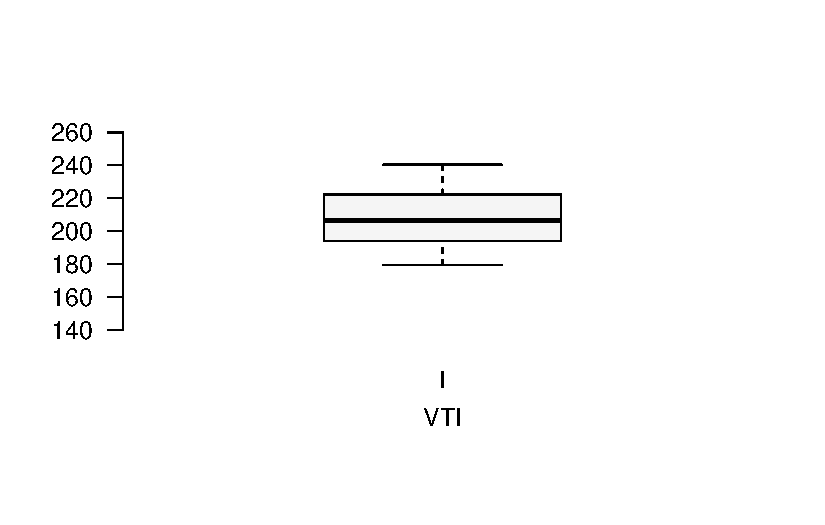
\includegraphics{./06-DescriptiveV_files/figure-pdf/unnamed-chunk-5-1.pdf}

}

\end{figure}

The boxplot shows that there are no outliers. The data also looks like
it has a slight skew to the right.

\begin{blackbox}

\begin{enumerate}
\def\labelenumi{\arabic{enumi}.}
\setcounter{enumi}{1}
\tightlist
\item
  The mean is more sensitive to outliers than the median. Hence, when
  the data is skewed to the right we expect that the mean is larger than
  the median.
\end{enumerate}

\end{blackbox}

Let's construct a histogram in R to search for skewness.

\begin{Shaded}
\begin{Highlighting}[numbers=left,,]
\FunctionTok{hist}\NormalTok{(StockPrices}\SpecialCharTok{$}\NormalTok{VTI,}\AttributeTok{main=}\StringTok{""}\NormalTok{, }\AttributeTok{ylim=}\FunctionTok{c}\NormalTok{(}\DecValTok{0}\NormalTok{,}\DecValTok{40}\NormalTok{), }
     \AttributeTok{xlab=}\StringTok{"Prices"}\NormalTok{, }\AttributeTok{col=}\StringTok{"\#F5F5F5"}\NormalTok{)}
\FunctionTok{abline}\NormalTok{(}\AttributeTok{v=}\FunctionTok{mean}\NormalTok{(StockPrices}\SpecialCharTok{$}\NormalTok{VTI),}\AttributeTok{col=}\StringTok{"black"}\NormalTok{,}\AttributeTok{lwd=}\DecValTok{2}\NormalTok{)}
\FunctionTok{abline}\NormalTok{(}\AttributeTok{v=}\FunctionTok{median}\NormalTok{(StockPrices}\SpecialCharTok{$}\NormalTok{VTI),}\AttributeTok{col=}\StringTok{"darkgrey"}\NormalTok{,}\AttributeTok{lwd=}\DecValTok{2}\NormalTok{)}
\FunctionTok{legend}\NormalTok{(}\AttributeTok{x =} \StringTok{"topright"}\NormalTok{,          }
       \AttributeTok{legend =} \FunctionTok{c}\NormalTok{(}\StringTok{"Mean"}\NormalTok{, }\StringTok{"Median"}\NormalTok{),  }
       \AttributeTok{lty =} \FunctionTok{c}\NormalTok{(}\DecValTok{1}\NormalTok{, }\DecValTok{1}\NormalTok{),           }
       \AttributeTok{col =} \FunctionTok{c}\NormalTok{(}\StringTok{"black"}\NormalTok{, }\StringTok{"darkgrey"}\NormalTok{),         }
       \AttributeTok{lwd =} \DecValTok{2}\NormalTok{,}
       \AttributeTok{bty=}\StringTok{"n"}\NormalTok{)    }
\end{Highlighting}
\end{Shaded}

\begin{figure}[H]

{\centering 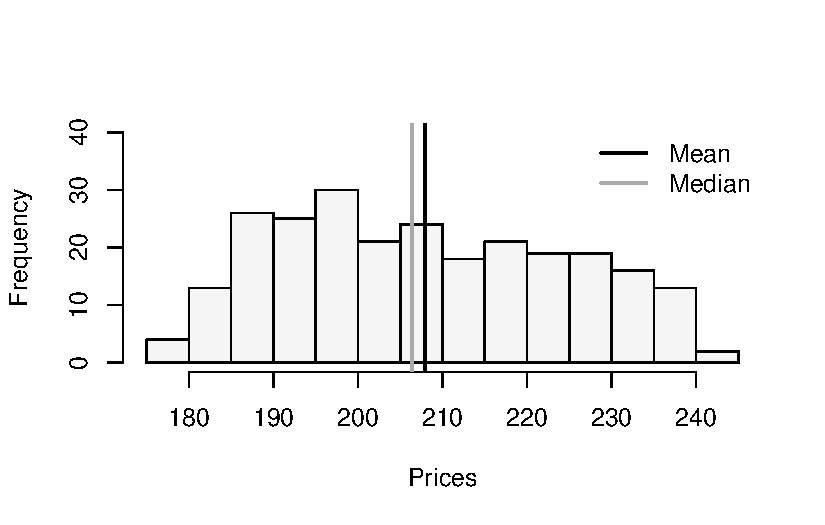
\includegraphics{./06-DescriptiveV_files/figure-pdf/unnamed-chunk-6-1.pdf}

}

\end{figure}

The lines are close to each other but the mean is slighlty larger than
the median. Let's confirm with the skewness statistic
\(3(mean-median)/sd\).

\begin{Shaded}
\begin{Highlighting}[numbers=left,,]
\NormalTok{(skew}\OtherTok{\textless{}{-}}\DecValTok{3}\SpecialCharTok{*}\NormalTok{(}\FunctionTok{mean}\NormalTok{(StockPrices}\SpecialCharTok{$}\NormalTok{VTI}\SpecialCharTok{{-}}\FunctionTok{median}\NormalTok{(StockPrices}\SpecialCharTok{$}\NormalTok{VTI))}\SpecialCharTok{/}\FunctionTok{sd}\NormalTok{(StockPrices}\SpecialCharTok{$}\NormalTok{VTI)))}
\end{Highlighting}
\end{Shaded}

\begin{verbatim}
[1] 0.2856304
\end{verbatim}

This indicates that there is a slight skew to the right of the data.

\begin{blackbox}

\begin{enumerate}
\def\labelenumi{\arabic{enumi}.}
\setcounter{enumi}{2}
\tightlist
\item
  The line chart indicates that the data has a downward trend in the
  early periods. This creates a few points that are large. In later
  periods the stock price stabilizes to lower levels.
\end{enumerate}

\end{blackbox}

\begin{Shaded}
\begin{Highlighting}[numbers=left,,]
\FunctionTok{plot}\NormalTok{(}\AttributeTok{y=}\NormalTok{StockPrices}\SpecialCharTok{$}\NormalTok{VTI,}\AttributeTok{x=}\FunctionTok{seq}\NormalTok{(}\DecValTok{1}\NormalTok{,}\FunctionTok{length}\NormalTok{(StockPrices}\SpecialCharTok{$}\NormalTok{VTI)),}
     \AttributeTok{type=}\StringTok{"l"}\NormalTok{, }\AttributeTok{ylab=}\StringTok{"Prices"}\NormalTok{, }\AttributeTok{xlab=}\StringTok{"Period"}\NormalTok{, }\AttributeTok{axes=}\NormalTok{F)}
\FunctionTok{axis}\NormalTok{(}\AttributeTok{side=}\DecValTok{1}\NormalTok{, }\AttributeTok{labels=}\ConstantTok{TRUE}\NormalTok{, }\AttributeTok{at=}\FunctionTok{seq}\NormalTok{(}\DecValTok{0}\NormalTok{,}\DecValTok{250}\NormalTok{,}\DecValTok{50}\NormalTok{),}\AttributeTok{font=}\DecValTok{1}\NormalTok{,}\AttributeTok{las=}\DecValTok{1}\NormalTok{)}
\FunctionTok{axis}\NormalTok{(}\AttributeTok{side=}\DecValTok{2}\NormalTok{, }\AttributeTok{labels=}\ConstantTok{TRUE}\NormalTok{, }\AttributeTok{at=}\FunctionTok{seq}\NormalTok{(}\DecValTok{0}\NormalTok{,}\DecValTok{300}\NormalTok{,}\DecValTok{20}\NormalTok{),}\AttributeTok{font=}\DecValTok{1}\NormalTok{,}\AttributeTok{las=}\DecValTok{1}\NormalTok{)}
\end{Highlighting}
\end{Shaded}

\begin{figure}[H]

{\centering 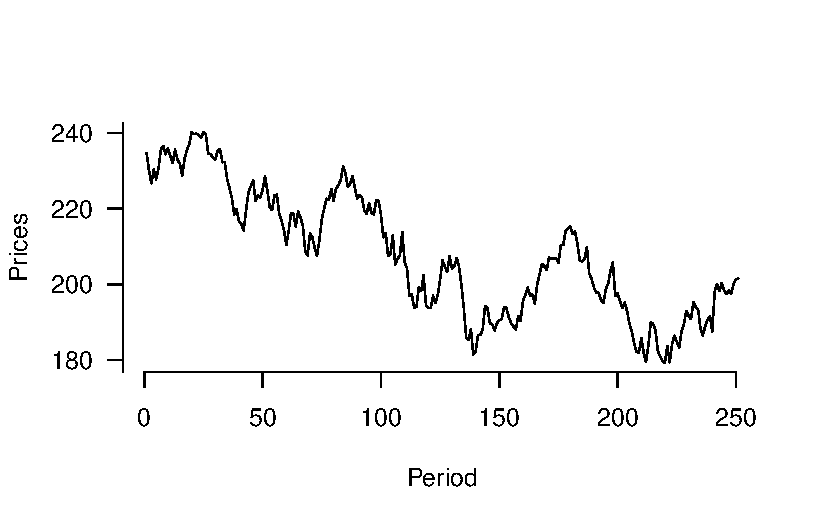
\includegraphics{./06-DescriptiveV_files/figure-pdf/unnamed-chunk-8-1.pdf}

}

\end{figure}

\hypertarget{exercise-3-9}{%
\subsection*{Exercise 3}\label{exercise-3-9}}
\addcontentsline{toc}{subsection}{Exercise 3}

\begin{blackbox}

\begin{enumerate}
\def\labelenumi{\arabic{enumi}.}
\tightlist
\item
  The outlier is the Masserati Bora. The horse power is \(335\).
\end{enumerate}

\end{blackbox}

In R we can construct a boxplot with the following command:

\begin{Shaded}
\begin{Highlighting}[numbers=left,,]
\FunctionTok{boxplot}\NormalTok{(mtcars}\SpecialCharTok{$}\NormalTok{hp,}\AttributeTok{axes=}\NormalTok{F, }\AttributeTok{ylim=}\FunctionTok{c}\NormalTok{(}\DecValTok{0}\NormalTok{,}\DecValTok{400}\NormalTok{),}
        \AttributeTok{cex=}\FloatTok{1.5}\NormalTok{, }\AttributeTok{col=}\StringTok{"\#F5F5F5"}\NormalTok{,}\AttributeTok{pch=}\DecValTok{21}\NormalTok{,}\AttributeTok{bg=}\StringTok{"red"}\NormalTok{)}
\FunctionTok{axis}\NormalTok{(}\AttributeTok{side=}\DecValTok{1}\NormalTok{, }\AttributeTok{labels=}\FunctionTok{c}\NormalTok{(}\StringTok{"HP"}\NormalTok{), }\AttributeTok{at=}\FunctionTok{seq}\NormalTok{(}\DecValTok{1}\NormalTok{))}
\FunctionTok{axis}\NormalTok{(}\AttributeTok{side=}\DecValTok{2}\NormalTok{, }\AttributeTok{labels=}\ConstantTok{TRUE}\NormalTok{, }\AttributeTok{at=}\FunctionTok{seq}\NormalTok{(}\DecValTok{0}\NormalTok{,}\DecValTok{400}\NormalTok{,}\DecValTok{50}\NormalTok{),}\AttributeTok{font=}\DecValTok{1}\NormalTok{,}\AttributeTok{las=}\DecValTok{1}\NormalTok{)}
\end{Highlighting}
\end{Shaded}

\begin{figure}[H]

{\centering 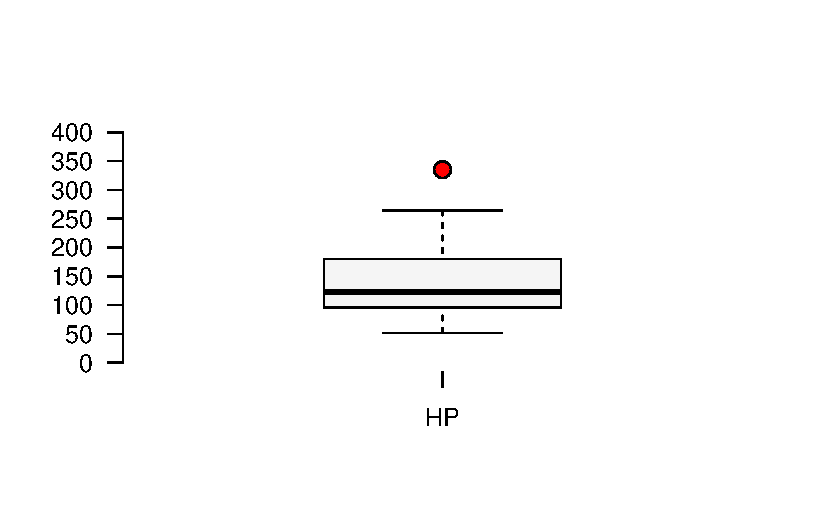
\includegraphics{./06-DescriptiveV_files/figure-pdf/unnamed-chunk-9-1.pdf}

}

\end{figure}

From the graph it seems like the outlier is beyond a horsepower of 275.
Let's write an R command to retrieve the car.

\begin{Shaded}
\begin{Highlighting}[numbers=left,,]
\NormalTok{mtcars[mtcars}\SpecialCharTok{$}\NormalTok{hp}\SpecialCharTok{\textgreater{}}\DecValTok{275}\NormalTok{,]}
\end{Highlighting}
\end{Shaded}

\begin{verbatim}
              mpg cyl disp  hp drat   wt qsec vs am gear carb
Maserati Bora  15   8  301 335 3.54 3.57 14.6  0  1    5    8
\end{verbatim}

It's the Masserati Bora!

\begin{blackbox}

\begin{enumerate}
\def\labelenumi{\arabic{enumi}.}
\setcounter{enumi}{1}
\tightlist
\item
  The histogram looks skewed to the right. This is confirmed by the
  estimation of a Pearson coefficient fo skewness of \(1.04\).
\end{enumerate}

\end{blackbox}

In R we can construct a histogram with vertical lines for the mean and
median wit the following code:

\begin{Shaded}
\begin{Highlighting}[numbers=left,,]
\FunctionTok{hist}\NormalTok{(mtcars}\SpecialCharTok{$}\NormalTok{hp,}\AttributeTok{main=}\StringTok{""}\NormalTok{, }\AttributeTok{ylim=}\FunctionTok{c}\NormalTok{(}\DecValTok{0}\NormalTok{,}\DecValTok{12}\NormalTok{), }\AttributeTok{xlab=}\StringTok{"Horse Power"}\NormalTok{,}
     \AttributeTok{col=}\StringTok{"\#F5F5F5"}\NormalTok{)}
\FunctionTok{abline}\NormalTok{(}\AttributeTok{v=}\FunctionTok{mean}\NormalTok{(mtcars}\SpecialCharTok{$}\NormalTok{hp),}\AttributeTok{col=}\StringTok{"black"}\NormalTok{,}\AttributeTok{lwd=}\DecValTok{2}\NormalTok{)}
\FunctionTok{abline}\NormalTok{(}\AttributeTok{v=}\FunctionTok{median}\NormalTok{(mtcars}\SpecialCharTok{$}\NormalTok{hp),}\AttributeTok{col=}\StringTok{"darkgrey"}\NormalTok{,}\AttributeTok{lwd=}\DecValTok{2}\NormalTok{)}
\FunctionTok{legend}\NormalTok{(}\AttributeTok{x =} \StringTok{"topright"}\NormalTok{,          }
       \AttributeTok{legend =} \FunctionTok{c}\NormalTok{(}\StringTok{"Mean"}\NormalTok{, }\StringTok{"Median"}\NormalTok{),  }
       \AttributeTok{lty =} \FunctionTok{c}\NormalTok{(}\DecValTok{1}\NormalTok{, }\DecValTok{1}\NormalTok{),           }
       \AttributeTok{col =} \FunctionTok{c}\NormalTok{(}\StringTok{"black"}\NormalTok{, }\StringTok{"darkgrey"}\NormalTok{),         }
       \AttributeTok{lwd =} \DecValTok{2}\NormalTok{,}
       \AttributeTok{bty=}\StringTok{"n"}\NormalTok{)    }
\end{Highlighting}
\end{Shaded}

\begin{figure}[H]

{\centering 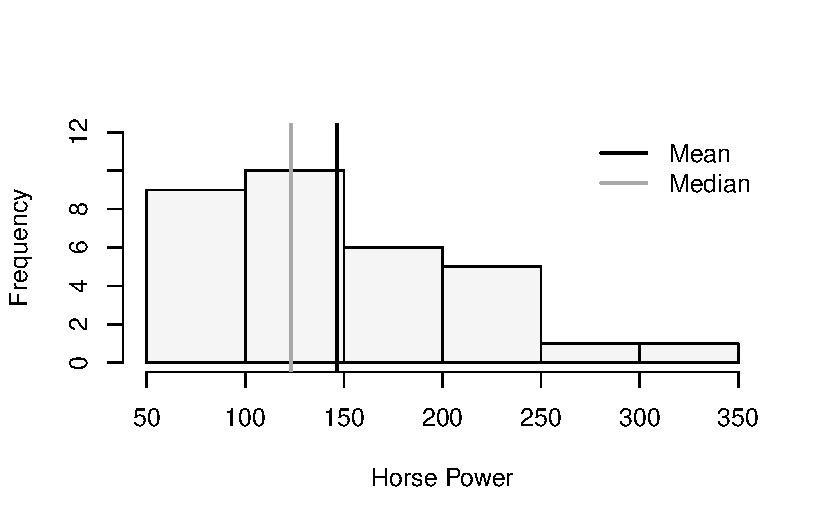
\includegraphics{./06-DescriptiveV_files/figure-pdf/unnamed-chunk-11-1.pdf}

}

\end{figure}

The histogram looks skewed to the right. Pearson's Coefficient of
Skewness is:

\begin{Shaded}
\begin{Highlighting}[numbers=left,,]
\NormalTok{(SkewHP}\OtherTok{\textless{}{-}}\DecValTok{3}\SpecialCharTok{*}\NormalTok{(}\FunctionTok{mean}\NormalTok{(mtcars}\SpecialCharTok{$}\NormalTok{hp)}\SpecialCharTok{{-}}\FunctionTok{median}\NormalTok{(mtcars}\SpecialCharTok{$}\NormalTok{hp))}\SpecialCharTok{/}\FunctionTok{sd}\NormalTok{(mtcars}\SpecialCharTok{$}\NormalTok{hp))}
\end{Highlighting}
\end{Shaded}

\begin{verbatim}
[1] 1.036458
\end{verbatim}

\begin{blackbox}

\begin{enumerate}
\def\labelenumi{\arabic{enumi}.}
\setcounter{enumi}{2}
\tightlist
\item
  The skew is still there, but the distribution now look more
  symmetrical and the Skew coefficient has decreased to \(0.44\).
\end{enumerate}

\end{blackbox}

In R we can create an new variable that captures the log transformation.
The \texttt{log()} function takes the natural logarithm of a number or
vector.

\begin{Shaded}
\begin{Highlighting}[numbers=left,,]
\NormalTok{LogHP}\OtherTok{\textless{}{-}}\FunctionTok{log}\NormalTok{(mtcars}\SpecialCharTok{$}\NormalTok{hp)}
\end{Highlighting}
\end{Shaded}

Let's use this new variable to create our histogram:

\begin{Shaded}
\begin{Highlighting}[numbers=left,,]
\FunctionTok{hist}\NormalTok{(LogHP,}\AttributeTok{main=}\StringTok{""}\NormalTok{, }\AttributeTok{ylim=}\FunctionTok{c}\NormalTok{(}\DecValTok{0}\NormalTok{,}\DecValTok{12}\NormalTok{), }\AttributeTok{xlab=}\StringTok{"Horse Power"}\NormalTok{, }
     \AttributeTok{col=}\StringTok{"\#F5F5F5"}\NormalTok{)}
\FunctionTok{abline}\NormalTok{(}\AttributeTok{v=}\FunctionTok{mean}\NormalTok{(LogHP),}\AttributeTok{col=}\StringTok{"black"}\NormalTok{,}\AttributeTok{lwd=}\DecValTok{2}\NormalTok{)}
\FunctionTok{abline}\NormalTok{(}\AttributeTok{v=}\FunctionTok{median}\NormalTok{(LogHP),}\AttributeTok{col=}\StringTok{"darkgrey"}\NormalTok{,}\AttributeTok{lwd=}\DecValTok{2}\NormalTok{)}
\FunctionTok{legend}\NormalTok{(}\AttributeTok{x =} \StringTok{"topright"}\NormalTok{,          }
       \AttributeTok{legend =} \FunctionTok{c}\NormalTok{(}\StringTok{"Mean"}\NormalTok{, }\StringTok{"Median"}\NormalTok{),  }
       \AttributeTok{lty =} \FunctionTok{c}\NormalTok{(}\DecValTok{1}\NormalTok{, }\DecValTok{1}\NormalTok{),           }
       \AttributeTok{col =} \FunctionTok{c}\NormalTok{(}\StringTok{"black"}\NormalTok{, }\StringTok{"darkgrey"}\NormalTok{),         }
       \AttributeTok{lwd =} \DecValTok{2}\NormalTok{,}
       \AttributeTok{bty=}\StringTok{"n"}\NormalTok{)    }
\end{Highlighting}
\end{Shaded}

\begin{figure}[H]

{\centering 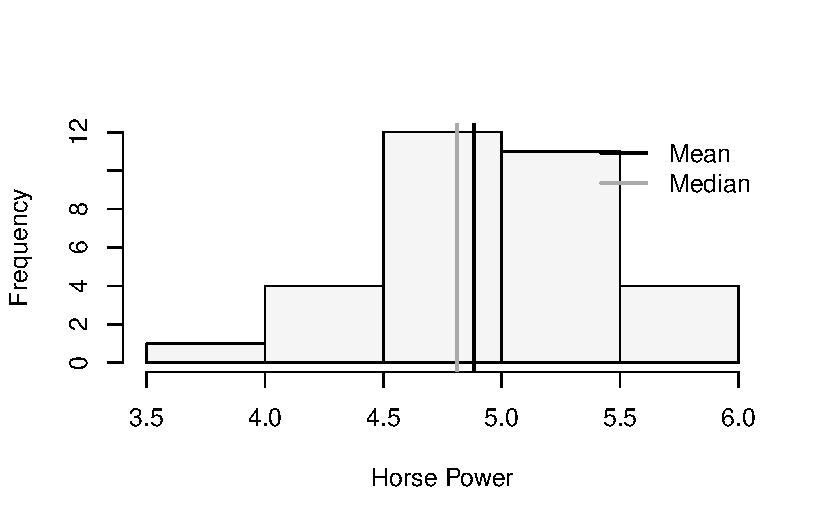
\includegraphics{./06-DescriptiveV_files/figure-pdf/unnamed-chunk-14-1.pdf}

}

\end{figure}

The mean and the variance now look closer together. The tail of the
distribution (skew) now also looks diminished. The Skewness coefficient
has decreased significantly:

\begin{Shaded}
\begin{Highlighting}[numbers=left,,]
\NormalTok{(SkewLogHP}\OtherTok{\textless{}{-}}\DecValTok{3}\SpecialCharTok{*}\NormalTok{(}\FunctionTok{mean}\NormalTok{(LogHP)}\SpecialCharTok{{-}}\FunctionTok{median}\NormalTok{(LogHP))}\SpecialCharTok{/}\FunctionTok{sd}\NormalTok{(LogHP))}
\end{Highlighting}
\end{Shaded}

\begin{verbatim}
[1] 0.4402212
\end{verbatim}

\part{Regression Estimation}

\hypertarget{regression-i}{%
\chapter{Regression I}\label{regression-i}}

\hypertarget{concepts-5}{%
\section{Concepts}\label{concepts-5}}

\hypertarget{measures-of-association}{%
\subsection*{Measures of Association}\label{measures-of-association}}
\addcontentsline{toc}{subsection}{Measures of Association}

Measures of association determine whether there is a linear relationship
between two variables. They also determine the strength of the
relationship.

\begin{itemize}
\item
  The \textbf{covariance} is a measure that determines the direction of
  the relationship between two variables. It is calculated by
  \(s_{xy}=\frac {\sum(x_i-\bar{x})(y_i-\bar{y})}{\sum (x_i-\bar{x})^2}\).
  If \(s_{xy}>0\) there is a direct relationship, if \(s_{xy}<0\) there
  is an inverse relationship, and if \(s_{xy}=0\) there is no
  relationship.
\item
  The \textbf{correlation} measures the strength of the linear
  relationship. It is calculated by \(r= \frac {s_{xy}}{s_x s_y}\). The
  correlation coefficient is between \([-1,1]\). When the correlation
  coefficient is \(1\) (\(-1\)), there is a perfect direct (inverse)
  relationship between the two variables.
\item
  The \textbf{coefficient of determination} or \(R^2\), measures the
  percent of variation in \(y\) explained by variations in \(x\). It is
  calculated by \(R^2=r^2\). The next chapter expands on this measure.
\item
  A \textbf{scatter plot} displays pairs of {[}\(x\),\(y\){]} as points
  on the Cartesian plane. The plot provides a visual aid to determine
  the relationship between two variables.
\end{itemize}

\hypertarget{useful-r-functions-5}{%
\subsection*{Useful R Functions}\label{useful-r-functions-5}}
\addcontentsline{toc}{subsection}{Useful R Functions}

To calculate the covariance use the \texttt{cov()} function.

The correlation coefficient can be calculated using the \texttt{cor()}
function.

The \texttt{plot()} function will create scatter plots.

\hypertarget{exercises-5}{%
\section{Exercises}\label{exercises-5}}

The following exercises will help you understand statistical measures
that establish the relationship between two variables. In particular,
the exercises work on:

\begin{itemize}
\item
  Calculating covariance and correlation.
\item
  Using R to plot scatter diagrams.
\item
  Calculating the coefficient of determination.
\end{itemize}

Answers are provided below. Try not to peak until you have a formulated
your own answer and double checked your work for any mistakes.

\hypertarget{exercise-1-10}{%
\subsection*{Exercise 1}\label{exercise-1-10}}
\addcontentsline{toc}{subsection}{Exercise 1}

For the following exercises, make your calculations by hand and verify
results using R functions when possible.

\begin{enumerate}
\def\labelenumi{\arabic{enumi}.}
\tightlist
\item
  Consider the data below. Calculate the covariance and correlation
  coefficient by finding deviations from the mean. Use R to verify your
  result. Is there a direct or inverse relationship between the two
  variables? How strong is the relationship?
\end{enumerate}

\begin{longtable}[]{@{}cccccc@{}}
\toprule()
\textbf{x} & 20 & 21 & 15 & 18 & 25 \\
\midrule()
\endhead
\textbf{y} & 17 & 19 & 12 & 13 & 22 \\
\bottomrule()
\end{longtable}

\begin{enumerate}
\def\labelenumi{\arabic{enumi}.}
\setcounter{enumi}{1}
\tightlist
\item
  Consider the data below. Calculate the covariance and correlation
  coefficient by finding deviations from the mean. Use R to verify your
  result. Is there a direct or inverse relationship between the two
  variables? How strong is the relationship?
\end{enumerate}

\begin{longtable}[]{@{}cccccc@{}}
\toprule()
\textbf{w} & 19 & 16 & 14 & 11 & 18 \\
\midrule()
\endhead
\textbf{z} & 17 & 20 & 20 & 16 & 18 \\
\bottomrule()
\end{longtable}

\hypertarget{exercise-2-10}{%
\subsection*{Exercise 2}\label{exercise-2-10}}
\addcontentsline{toc}{subsection}{Exercise 2}

You will need the \textbf{mtcars} data set to answer this question. This
data set is part of R. You don't need to download any files to access
it.

\begin{enumerate}
\def\labelenumi{\arabic{enumi}.}
\item
  Calculate the correlation coefficient between \emph{hp} and
  \emph{mpg}. Explain the results. Specifically, the direction of the
  relationship and the strength given the context of the problem.
\item
  Create a scatter diagram of the two variables. Is the scatter diagram
  what you expected after you calculated the correlation coefficient?
\item
  Calculate the coefficient of determination. How close is it to one?
  What else could be explaining the variation in the \emph{mpg}? Let
  your dependent variable be \emph{mpg}.
\end{enumerate}

\hypertarget{exercise-3-10}{%
\subsection*{Exercise 3}\label{exercise-3-10}}
\addcontentsline{toc}{subsection}{Exercise 3}

You will need the \textbf{College} data set to answer this question. You
can find this data set here: https://jagelves.github.io/Data/College.csv

\begin{enumerate}
\def\labelenumi{\arabic{enumi}.}
\item
  Create a scatter diagram between \emph{GRAD\_DEBT\_MDN} (Median Debt)
  and \emph{MD\_EARN\_WNE\_P10} (Median Earnings). What type of
  relationship do you observe between the variables?
\item
  Calculate the correlation coefficient and the coefficient of
  determination. According to the data, are higher debts correlated with
  higher earnings?
\end{enumerate}

\hypertarget{answers-5}{%
\section{Answers}\label{answers-5}}

\hypertarget{exercise-1-11}{%
\subsection*{Exercise 1}\label{exercise-1-11}}
\addcontentsline{toc}{subsection}{Exercise 1}

\begin{blackbox}

\begin{enumerate}
\def\labelenumi{\arabic{enumi}.}
\tightlist
\item
  The covariance is \(14.9\) and the correlation is \(0.96\). The
  results indicate that there is a strong direct relationship between
  the two variables.
\end{enumerate}

\end{blackbox}

Let's start by finding the deviations from the mean for the \emph{x}
variable in R.

\begin{Shaded}
\begin{Highlighting}[numbers=left,,]
\NormalTok{x}\OtherTok{\textless{}{-}}\FunctionTok{c}\NormalTok{(}\DecValTok{20}\NormalTok{,}\DecValTok{21}\NormalTok{,}\DecValTok{15}\NormalTok{,}\DecValTok{18}\NormalTok{,}\DecValTok{25}\NormalTok{)}
\NormalTok{(devx}\OtherTok{\textless{}{-}}\NormalTok{x}\SpecialCharTok{{-}}\FunctionTok{mean}\NormalTok{(x))}
\end{Highlighting}
\end{Shaded}

\begin{verbatim}
[1]  0.2  1.2 -4.8 -1.8  5.2
\end{verbatim}

We will do the same with y:

\begin{Shaded}
\begin{Highlighting}[numbers=left,,]
\NormalTok{y}\OtherTok{\textless{}{-}}\FunctionTok{c}\NormalTok{(}\DecValTok{17}\NormalTok{,}\DecValTok{19}\NormalTok{,}\DecValTok{12}\NormalTok{,}\DecValTok{13}\NormalTok{,}\DecValTok{22}\NormalTok{)}
\NormalTok{(devy}\OtherTok{\textless{}{-}}\NormalTok{y}\SpecialCharTok{{-}}\FunctionTok{mean}\NormalTok{(y))}
\end{Highlighting}
\end{Shaded}

\begin{verbatim}
[1]  0.4  2.4 -4.6 -3.6  5.4
\end{verbatim}

Note that when the deviations in \emph{x} are negative (positive), they
are also negative (positive) in \emph{y}. This is indicative of a direct
relationship between the two variables. The covariance is given by:

\begin{Shaded}
\begin{Highlighting}[numbers=left,,]
\NormalTok{(Ex1Cov}\OtherTok{\textless{}{-}}\FunctionTok{sum}\NormalTok{(devx}\SpecialCharTok{*}\NormalTok{devy)}\SpecialCharTok{/}\NormalTok{(}\FunctionTok{length}\NormalTok{(devx)}\SpecialCharTok{{-}}\DecValTok{1}\NormalTok{))}
\end{Highlighting}
\end{Shaded}

\begin{verbatim}
[1] 14.9
\end{verbatim}

We can verify this by using \texttt{cov()} function in R.

\begin{Shaded}
\begin{Highlighting}[numbers=left,,]
\FunctionTok{cov}\NormalTok{(x,y)}
\end{Highlighting}
\end{Shaded}

\begin{verbatim}
[1] 14.9
\end{verbatim}

The correlation coefficient is found by dividing the covariance over the
product of standard deviations. In R:

\begin{Shaded}
\begin{Highlighting}[numbers=left,,]
\NormalTok{(Ex1Cor}\OtherTok{\textless{}{-}}\NormalTok{Ex1Cov}\SpecialCharTok{/}\NormalTok{(}\FunctionTok{sd}\NormalTok{(x)}\SpecialCharTok{*}\FunctionTok{sd}\NormalTok{(y)))}
\end{Highlighting}
\end{Shaded}

\begin{verbatim}
[1] 0.9678386
\end{verbatim}

We can once more verify the result in R with the built in function
\texttt{cor()}.

\begin{Shaded}
\begin{Highlighting}[numbers=left,,]
\FunctionTok{cor}\NormalTok{(x,y)}
\end{Highlighting}
\end{Shaded}

\begin{verbatim}
[1] 0.9678386
\end{verbatim}

\begin{blackbox}

\begin{enumerate}
\def\labelenumi{\arabic{enumi}.}
\setcounter{enumi}{1}
\tightlist
\item
  The covariance is \(0.85\) and the correlation is \(0.148\). The
  results indicate that there is a very weak direct relationship between
  the two variables. They might be unrelated.
\end{enumerate}

\end{blackbox}

Let's start with \emph{w} and finding the deviations from the mean in R.

\begin{Shaded}
\begin{Highlighting}[numbers=left,,]
\NormalTok{w}\OtherTok{\textless{}{-}}\FunctionTok{c}\NormalTok{(}\DecValTok{19}\NormalTok{,}\DecValTok{16}\NormalTok{,}\DecValTok{14}\NormalTok{,}\DecValTok{11}\NormalTok{,}\DecValTok{18}\NormalTok{)}
\NormalTok{(devw}\OtherTok{\textless{}{-}}\NormalTok{w}\SpecialCharTok{{-}}\FunctionTok{mean}\NormalTok{(w))}
\end{Highlighting}
\end{Shaded}

\begin{verbatim}
[1]  3.4  0.4 -1.6 -4.6  2.4
\end{verbatim}

We will do the same with \emph{z}:

\begin{Shaded}
\begin{Highlighting}[numbers=left,,]
\NormalTok{z}\OtherTok{\textless{}{-}}\FunctionTok{c}\NormalTok{(}\DecValTok{17}\NormalTok{,}\DecValTok{20}\NormalTok{,}\DecValTok{20}\NormalTok{,}\DecValTok{16}\NormalTok{,}\DecValTok{18}\NormalTok{)}
\NormalTok{(devz}\OtherTok{\textless{}{-}}\NormalTok{z}\SpecialCharTok{{-}}\FunctionTok{mean}\NormalTok{(z))}
\end{Highlighting}
\end{Shaded}

\begin{verbatim}
[1] -1.2  1.8  1.8 -2.2 -0.2
\end{verbatim}

The covariance is given by:

\begin{Shaded}
\begin{Highlighting}[numbers=left,,]
\NormalTok{(Ex2Cov}\OtherTok{\textless{}{-}}\FunctionTok{sum}\NormalTok{(devw}\SpecialCharTok{*}\NormalTok{devz)}\SpecialCharTok{/}\NormalTok{(}\FunctionTok{length}\NormalTok{(devz)}\SpecialCharTok{{-}}\DecValTok{1}\NormalTok{))}
\end{Highlighting}
\end{Shaded}

\begin{verbatim}
[1] 0.85
\end{verbatim}

We can verify this with the \texttt{cov()} function in R.

\begin{Shaded}
\begin{Highlighting}[numbers=left,,]
\FunctionTok{cov}\NormalTok{(w,z)}
\end{Highlighting}
\end{Shaded}

\begin{verbatim}
[1] 0.85
\end{verbatim}

The correlation coefficient is found by dividing the covariance over the
product of standard deviations. In R:

\begin{Shaded}
\begin{Highlighting}[numbers=left,,]
\NormalTok{(Ex2Cor}\OtherTok{\textless{}{-}}\NormalTok{Ex2Cov}\SpecialCharTok{/}\NormalTok{(}\FunctionTok{sd}\NormalTok{(z)}\SpecialCharTok{*}\FunctionTok{sd}\NormalTok{(w)))}
\end{Highlighting}
\end{Shaded}

\begin{verbatim}
[1] 0.1480558
\end{verbatim}

We can once more verify the result in R with the built in function
\texttt{cor()}.

\begin{Shaded}
\begin{Highlighting}[numbers=left,,]
\FunctionTok{cor}\NormalTok{(w,z)}
\end{Highlighting}
\end{Shaded}

\begin{verbatim}
[1] 0.1480558
\end{verbatim}

\hypertarget{exercise-2-11}{%
\subsection*{Exercise 2}\label{exercise-2-11}}
\addcontentsline{toc}{subsection}{Exercise 2}

\begin{blackbox}

\begin{enumerate}
\def\labelenumi{\arabic{enumi}.}
\tightlist
\item
  The correlation coefficient is \(-0.78\). This is indicative of a
  moderately strong inverse relationship between \emph{mpg} and
  \emph{mp}.
\end{enumerate}

\end{blackbox}

In R we can easily calculate the correlation coefficient with the
\texttt{cor()} function.

\begin{Shaded}
\begin{Highlighting}[numbers=left,,]
\FunctionTok{cor}\NormalTok{(mtcars}\SpecialCharTok{$}\NormalTok{mpg,mtcars}\SpecialCharTok{$}\NormalTok{hp)}
\end{Highlighting}
\end{Shaded}

\begin{verbatim}
[1] -0.7761684
\end{verbatim}

\begin{blackbox}

\begin{enumerate}
\def\labelenumi{\arabic{enumi}.}
\setcounter{enumi}{1}
\tightlist
\item
  The scatter diagram is downward sloping. Most points are close to the
  trend line. It is what was expected from a correlation coefficient of
  \(-0.78\).
\end{enumerate}

\end{blackbox}

\begin{Shaded}
\begin{Highlighting}[numbers=left,,]
\FunctionTok{plot}\NormalTok{(}\AttributeTok{y=}\NormalTok{mtcars}\SpecialCharTok{$}\NormalTok{mpg,}\AttributeTok{x=}\NormalTok{mtcars}\SpecialCharTok{$}\NormalTok{hp, }\AttributeTok{main=}\StringTok{""}\NormalTok{, }
     \AttributeTok{axes=}\NormalTok{F,}\AttributeTok{pch=}\DecValTok{21}\NormalTok{, }\AttributeTok{bg=}\StringTok{"blue"}\NormalTok{,}
     \AttributeTok{xlab=}\StringTok{"Horse Power"}\NormalTok{,}
     \AttributeTok{ylab=}\StringTok{"Miles Per Gallon"}\NormalTok{, }\AttributeTok{ylim=}\FunctionTok{c}\NormalTok{(}\DecValTok{10}\NormalTok{,}\DecValTok{40}\NormalTok{),}\AttributeTok{xlim=}\FunctionTok{c}\NormalTok{(}\DecValTok{50}\NormalTok{,}\DecValTok{400}\NormalTok{))}
\FunctionTok{axis}\NormalTok{(}\AttributeTok{side=}\DecValTok{1}\NormalTok{, }\AttributeTok{labels=}\ConstantTok{TRUE}\NormalTok{, }\AttributeTok{font=}\DecValTok{1}\NormalTok{,}\AttributeTok{las=}\DecValTok{1}\NormalTok{)}
\FunctionTok{axis}\NormalTok{(}\AttributeTok{side=}\DecValTok{2}\NormalTok{, }\AttributeTok{labels=}\ConstantTok{TRUE}\NormalTok{, }\AttributeTok{font=}\DecValTok{1}\NormalTok{,}\AttributeTok{las=}\DecValTok{1}\NormalTok{)}
\FunctionTok{abline}\NormalTok{(}\FunctionTok{lm}\NormalTok{(mtcars}\SpecialCharTok{$}\NormalTok{mpg}\SpecialCharTok{\textasciitilde{}}\NormalTok{mtcars}\SpecialCharTok{$}\NormalTok{hp),}
       \AttributeTok{col=}\StringTok{"darkgray"}\NormalTok{,}\AttributeTok{lwd=}\DecValTok{2}\NormalTok{)}
\end{Highlighting}
\end{Shaded}

\begin{figure}[H]

{\centering 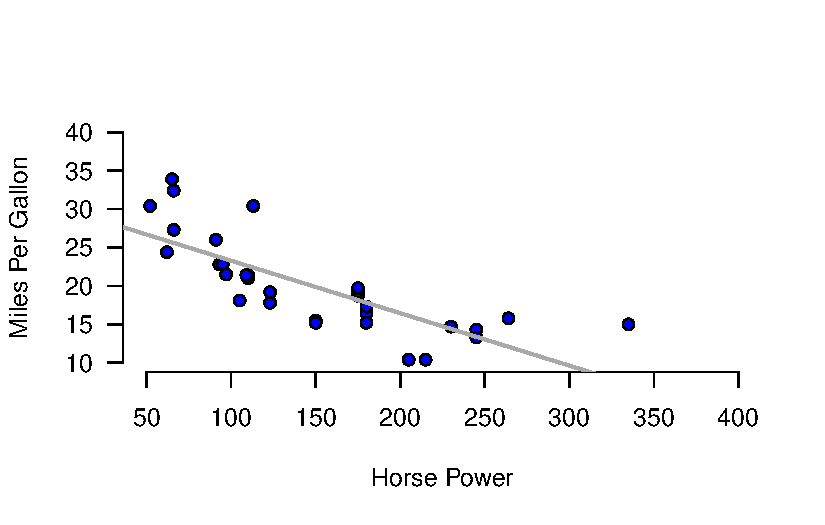
\includegraphics{./07-RegressionI_files/figure-pdf/unnamed-chunk-14-1.pdf}

}

\end{figure}

\begin{blackbox}

\begin{enumerate}
\def\labelenumi{\arabic{enumi}.}
\setcounter{enumi}{2}
\tightlist
\item
  The coefficient of determination is \(0.6\). This value is not very
  close to one. This is expected since miles per gallon can also vary
  because of the cars weight, and fuel efficiency. It makes sense that
  the \emph{hp} only explains \(60\)\% of the total variation.
\end{enumerate}

\end{blackbox}

In R we can calculate the coefficient of determination by squaring the
correlation coefficient.

\begin{Shaded}
\begin{Highlighting}[numbers=left,,]
\FunctionTok{cor}\NormalTok{(mtcars}\SpecialCharTok{$}\NormalTok{mpg,mtcars}\SpecialCharTok{$}\NormalTok{hp)}\SpecialCharTok{\^{}}\DecValTok{2}
\end{Highlighting}
\end{Shaded}

\begin{verbatim}
[1] 0.6024373
\end{verbatim}

\hypertarget{exercise-3-11}{%
\subsection*{Exercise 3}\label{exercise-3-11}}
\addcontentsline{toc}{subsection}{Exercise 3}

\begin{blackbox}

\begin{enumerate}
\def\labelenumi{\arabic{enumi}.}
\tightlist
\item
  It seems like there is a direct relationship between both variables.
  The more debt you take, the higher the salary.
\end{enumerate}

\end{blackbox}

Start by loading the data. We'll use the \texttt{read.csv()} function:

\begin{Shaded}
\begin{Highlighting}[numbers=left,,]
\NormalTok{College}\OtherTok{\textless{}{-}}\FunctionTok{read.csv}\NormalTok{(}\StringTok{"https://jagelves.github.io/Data/College.csv"}\NormalTok{)}
\end{Highlighting}
\end{Shaded}

The two variables of interest are \emph{GRAD\_DEBT\_MDN} and
\emph{MD\_EARN\_WNE\_P10}. The following code creates the scatter plot:

\begin{Shaded}
\begin{Highlighting}[numbers=left,,]
\FunctionTok{plot}\NormalTok{(}\AttributeTok{y=}\NormalTok{College}\SpecialCharTok{$}\NormalTok{MD\_EARN\_WNE\_P10, }\AttributeTok{x=}\NormalTok{College}\SpecialCharTok{$}\NormalTok{GRAD\_DEBT\_MDN, }
     \AttributeTok{main=}\StringTok{""}\NormalTok{, }\AttributeTok{axes=}\NormalTok{F, }\AttributeTok{pch=}\DecValTok{21}\NormalTok{, }\AttributeTok{bg=}\StringTok{"blue"}\NormalTok{,}
     \AttributeTok{xlab=}\StringTok{"Earnings"}\NormalTok{,}\AttributeTok{ylab=}\StringTok{"Debt"}\NormalTok{)}
\FunctionTok{axis}\NormalTok{(}\AttributeTok{side=}\DecValTok{1}\NormalTok{, }\AttributeTok{labels=}\ConstantTok{TRUE}\NormalTok{, }\AttributeTok{font=}\DecValTok{1}\NormalTok{,}\AttributeTok{las=}\DecValTok{1}\NormalTok{)}
\FunctionTok{axis}\NormalTok{(}\AttributeTok{side=}\DecValTok{2}\NormalTok{, }\AttributeTok{labels=}\ConstantTok{TRUE}\NormalTok{, }\AttributeTok{font=}\DecValTok{1}\NormalTok{,}\AttributeTok{las=}\DecValTok{1}\NormalTok{)}
\FunctionTok{abline}\NormalTok{(}\FunctionTok{lm}\NormalTok{(MD\_EARN\_WNE\_P10}\SpecialCharTok{\textasciitilde{}}\NormalTok{GRAD\_DEBT\_MDN, }\AttributeTok{data=}\NormalTok{College),}
       \AttributeTok{col=}\StringTok{"darkgrey"}\NormalTok{,}\AttributeTok{lwd=}\DecValTok{2}\NormalTok{)}
\end{Highlighting}
\end{Shaded}

\begin{figure}[H]

{\centering 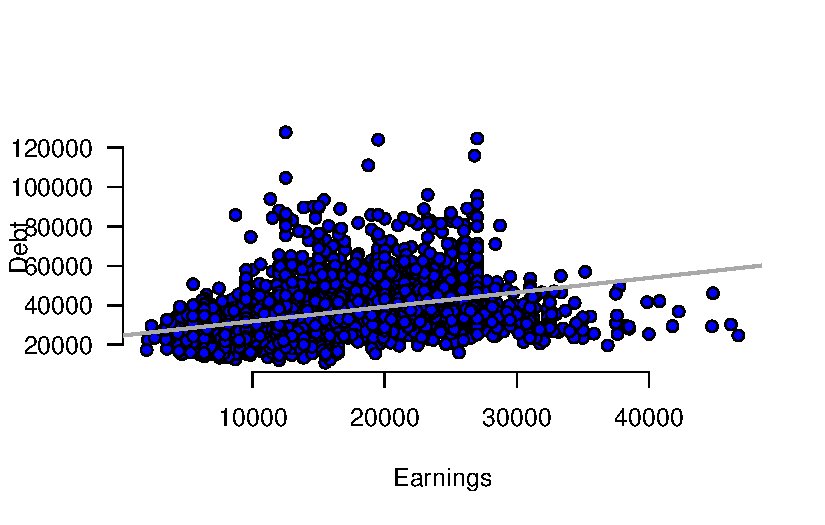
\includegraphics{./07-RegressionI_files/figure-pdf/unnamed-chunk-17-1.pdf}

}

\end{figure}

\begin{blackbox}

\begin{enumerate}
\def\labelenumi{\arabic{enumi}.}
\setcounter{enumi}{1}
\tightlist
\item
  The correlation coefficient shows a moderate direct relationship
  between earnings and debt \(0.43\). The coefficient of determination
  indicates that only \(19\)\% of the variation in earnings can be
  explained by debt.
\end{enumerate}

\end{blackbox}

In R we can start with the correlation coefficient:

\begin{Shaded}
\begin{Highlighting}[numbers=left,,]
\FunctionTok{cor}\NormalTok{(College}\SpecialCharTok{$}\NormalTok{MD\_EARN\_WNE\_P10,College}\SpecialCharTok{$}\NormalTok{GRAD\_DEBT\_MDN)}
\end{Highlighting}
\end{Shaded}

\begin{verbatim}
[1] 0.4328106
\end{verbatim}

The coefficient of determination is:

\begin{Shaded}
\begin{Highlighting}[numbers=left,,]
\FunctionTok{cor}\NormalTok{(College}\SpecialCharTok{$}\NormalTok{MD\_EARN\_WNE\_P10,College}\SpecialCharTok{$}\NormalTok{GRAD\_DEBT\_MDN)}\SpecialCharTok{\^{}}\DecValTok{2}
\end{Highlighting}
\end{Shaded}

\begin{verbatim}
[1] 0.187325
\end{verbatim}

\hypertarget{regression-ii}{%
\chapter{Regression II}\label{regression-ii}}

\hypertarget{concepts-6}{%
\section{Concepts}\label{concepts-6}}

\hypertarget{the-regression-line}{%
\subsection*{The Regression Line}\label{the-regression-line}}
\addcontentsline{toc}{subsection}{The Regression Line}

The regression line is fitted so that the average distance between the
line and the sample points is as small as possible. The line is defined
by a \textbf{slope} (\(\beta\)) and an \textbf{intercept} (\(\alpha\)).
Mathematically, the regression line is expressed as
\(\hat{y_i}=\hat{\alpha}+\hat{\beta}x_i\), where \(\hat{y_i}\) are the
predicted values of \(y\) given the \(x\)'s.

\begin{itemize}
\item
  The \textbf{slope} determines the steepness of the line. The estimate
  quantifies how much a unit increase in \(x\) changes \(y\). The
  estimate is given by \(\hat{\beta}= \frac {s_{xy}}{s_{x}^2}\).
\item
  The \textbf{intercept} determines where the line crosses the \(y\)
  axis. It returns the value of \(y\) when \(x\) is zero. The estimate
  is given by \(\hat{\alpha}=\bar{y}-\hat{\beta}\bar{x}\).
\end{itemize}

\hypertarget{goodness-of-fit}{%
\subsection*{Goodness of Fit}\label{goodness-of-fit}}
\addcontentsline{toc}{subsection}{Goodness of Fit}

There are a couple of popular measures that determine the goodness of
fit of the regression line.

\begin{itemize}
\item
  The \textbf{coefficient of determination} or \(R^2\) is the percent of
  the variation in \(y\) that is explained by changes in \(x\). The
  higher the \(R^2\) the better the explanatory power of the model. The
  \(R^2\) is always between {[}0,1{]}. To calculate use \(R^2=SSR/SST\).

  \begin{itemize}
  \item
    \(SSR\) (Sum of Squares due to Regression) is the part of the
    variation in \(y\) explained by the model. Mathematically,
    \(SSR=\sum{(\hat{y_i}-\bar{y})^2}\).
  \item
    \(SSE\) (Sum of Squares due to Error) is the part of the variation
    in \(y\) that is unexplained by the model. Mathematically,
    \(SSE=\sum{(y_i-\hat{y_i})^2}\).
  \item
    SST (Sum of Squares Total) is the total variation of \(y\) with
    respect to the mean. Mathematically, \(SST=\sum{(y_i-\bar{y})^2}\).
  \item
    Note that \(SST=SSR+SSE\).
  \end{itemize}
\item
  The \textbf{adjusted} \(R^2\) recognizes that the \(R^2\) is a
  non-decreasing function of the number of explanatory variables in the
  model. This metric penalizes a model with more explanatory variables
  relative to a simpler model. It is calculated by
  \(1-(1-R^2) \frac {n-1}{n-k-1}\), where \(k\) is the number of
  explanatory variables used in the model and \(n\) is the sample size.
\item
  The \textbf{Residual Standard Error} estimates the average dispersion
  of the data points around the regression line. It is calculated by
  \(s_e =\sqrt{\frac{SSE}{n-k-1}}\).
\end{itemize}

\hypertarget{useful-r-functions-6}{%
\subsection*{Useful R Functions}\label{useful-r-functions-6}}
\addcontentsline{toc}{subsection}{Useful R Functions}

The \texttt{lm()} function to estimates the linear regression model.

The \texttt{predict()} function uses the linear model object to predict
values. New data is entered as a data frame.

The \texttt{coef()} function returns the model's coefficients.

The \texttt{summary()} function returns the model's coefficients, and
goodness of fit measures.

\hypertarget{exercises-6}{%
\section{Exercises}\label{exercises-6}}

The following exercises will help you get practice on Regression Line
estimation and interpretation. In particular, the exercises work on:

\begin{itemize}
\item
  Estimating the slope and intercept.
\item
  Calculating measures of goodness of fit.
\item
  Prediction using the regression line.
\end{itemize}

Answers are provided below. Try not to peak until you have a formulated
your own answer and double checked your work for any mistakes.

\hypertarget{exercise-1-12}{%
\subsection*{Exercise 1}\label{exercise-1-12}}
\addcontentsline{toc}{subsection}{Exercise 1}

For the following exercises, make your calculations by hand and verify
results using R functions when possible.

\begin{enumerate}
\def\labelenumi{\arabic{enumi}.}
\tightlist
\item
  Consider the data below. Calculate the deviations from the mean for
  each variable and use the results to estimate the regression line. Use
  R to verify your result. On average by how much does \emph{y} increase
  per unit increase of \emph{x}?
\end{enumerate}

\begin{longtable}[]{@{}cccccc@{}}
\toprule()
\textbf{x} & 20 & 21 & 15 & 18 & 25 \\
\midrule()
\endhead
\textbf{y} & 17 & 19 & 12 & 13 & 22 \\
\bottomrule()
\end{longtable}

\begin{enumerate}
\def\labelenumi{\arabic{enumi}.}
\setcounter{enumi}{1}
\item
  Calculate \emph{SST}, \emph{SSR}, and \emph{SSE}. Confirm your results
  in R. What is the \(R^2\)? What is the Standard Error estimate? Is the
  regression line a good fit for the data?
\item
  Assume that \emph{x} is observed to be \emph{32}, what is your
  prediction of \emph{y}? How confident are you in this prediction?
\end{enumerate}

\hypertarget{exercise-2-12}{%
\subsection*{Exercise 2}\label{exercise-2-12}}
\addcontentsline{toc}{subsection}{Exercise 2}

You will need the \textbf{Education} data set to answer this question.
You can find the data set at
https://jagelves.github.io/Data/Education.csv . The data shows the years
of education (\emph{Education}), and annual salary in thousands
(\emph{Salary}) for a sample of \(100\) people.

\begin{enumerate}
\def\labelenumi{\arabic{enumi}.}
\item
  Estimate the regression line using R. By how much does an extra year
  of education increase the annual salary on average? What is the salary
  of someone without any education?
\item
  Confirm that the regression line is a good fit for the data. What is
  the estimated salary of a person with \(16\) years of education?
\end{enumerate}

\hypertarget{exercise-3-12}{%
\subsection*{Exercise 3}\label{exercise-3-12}}
\addcontentsline{toc}{subsection}{Exercise 3}

You will need the \textbf{FoodSpend} data set to answer this question.
You can find this data set at
https://jagelves.github.io/Data/FoodSpend.csv .

\begin{enumerate}
\def\labelenumi{\arabic{enumi}.}
\item
  Omit any NA's that the data has. Create a dummy variable that is equal
  to \(1\) if an individual owns a home and \(0\) if the individual
  doesn't. Find the mean of your dummy variable. What proportion of the
  sample owns a home?
\item
  Run a regression with \emph{Food} being the dependent variable and
  your dummy variable as the independent variable. What is the
  interpretation of the intercept and slope?
\item
  Now run a regression with \emph{Food} being the independent variable
  and your dummy variable as the dependent variable. What is the
  interpretation of the intercept and slope? Hint: you might want to
  plot the scatter diagram and the regression line.
\end{enumerate}

\hypertarget{exercise-4-2}{%
\subsection*{Exercise 4}\label{exercise-4-2}}
\addcontentsline{toc}{subsection}{Exercise 4}

You will need the \textbf{Population} data set to answer this question.
You can find this data set at
https://jagelves.github.io/Data/Population.csv .

\begin{enumerate}
\def\labelenumi{\arabic{enumi}.}
\item
  Run a regression of \emph{Population} on \emph{Year}. How well does
  the regression line fit the data?
\item
  Create a prediction for Japan's population in 2030. What is your
  prediction?
\item
  Create a scatter diagram and include the regression line. How
  confident are you of your prediction after looking at the diagram?
\end{enumerate}

\hypertarget{answers-6}{%
\section{Answers}\label{answers-6}}

\hypertarget{exercise-1-13}{%
\subsection*{Exercise 1}\label{exercise-1-13}}
\addcontentsline{toc}{subsection}{Exercise 1}

\begin{blackbox}

\begin{enumerate}
\def\labelenumi{\arabic{enumi}.}
\tightlist
\item
  The regression lines is \(\hat{y}=-4.93+1.09x\). For each unit
  increase in \emph{x}, \emph{y} increases on average \(1.09\).
\end{enumerate}

\end{blackbox}

Start by generating the deviations from the mean for each variable. For
\emph{x} the deviations are:

\begin{Shaded}
\begin{Highlighting}[numbers=left,,]
\NormalTok{x}\OtherTok{\textless{}{-}}\FunctionTok{c}\NormalTok{(}\DecValTok{20}\NormalTok{,}\DecValTok{21}\NormalTok{,}\DecValTok{15}\NormalTok{,}\DecValTok{18}\NormalTok{,}\DecValTok{25}\NormalTok{)}
\NormalTok{(devx}\OtherTok{\textless{}{-}}\NormalTok{x}\SpecialCharTok{{-}}\FunctionTok{mean}\NormalTok{(x))}
\end{Highlighting}
\end{Shaded}

\begin{verbatim}
[1]  0.2  1.2 -4.8 -1.8  5.2
\end{verbatim}

Next, find the deviations for \emph{y}:

\begin{Shaded}
\begin{Highlighting}[numbers=left,,]
\NormalTok{y}\OtherTok{\textless{}{-}}\FunctionTok{c}\NormalTok{(}\DecValTok{17}\NormalTok{,}\DecValTok{19}\NormalTok{,}\DecValTok{12}\NormalTok{,}\DecValTok{13}\NormalTok{,}\DecValTok{22}\NormalTok{)}
\NormalTok{(devy}\OtherTok{\textless{}{-}}\NormalTok{y}\SpecialCharTok{{-}}\FunctionTok{mean}\NormalTok{(y))}
\end{Highlighting}
\end{Shaded}

\begin{verbatim}
[1]  0.4  2.4 -4.6 -3.6  5.4
\end{verbatim}

For the slope we need to find the deviation squared of the \emph{x}'s.
This can easily be done in R:

\begin{Shaded}
\begin{Highlighting}[numbers=left,,]
\NormalTok{(devx2}\OtherTok{\textless{}{-}}\NormalTok{devx}\SpecialCharTok{\^{}}\DecValTok{2}\NormalTok{)}
\end{Highlighting}
\end{Shaded}

\begin{verbatim}
[1]  0.04  1.44 23.04  3.24 27.04
\end{verbatim}

The slope is calculated by
\(\frac{\sum_{i=i}^{n} (x_{i}-\bar{x})(y_{i}-\bar{y})}{\sum_{i=i}^{n} (x_{i}-\bar{x})^2}\).
In R we can just find the ratio between the summations of
\emph{(devx)(devy)} and \emph{devx2}.

\begin{Shaded}
\begin{Highlighting}[numbers=left,,]
\NormalTok{(slope}\OtherTok{\textless{}{-}}\FunctionTok{sum}\NormalTok{(devx}\SpecialCharTok{*}\NormalTok{devy)}\SpecialCharTok{/}\FunctionTok{sum}\NormalTok{(devx2))}
\end{Highlighting}
\end{Shaded}

\begin{verbatim}
[1] 1.087591
\end{verbatim}

The intercept is given by \(\bar{y}-\beta(\bar{x})\). In R we find that
the intercept is equal to:

\begin{Shaded}
\begin{Highlighting}[numbers=left,,]
\NormalTok{(intercept}\OtherTok{\textless{}{-}}\FunctionTok{mean}\NormalTok{(y)}\SpecialCharTok{{-}}\NormalTok{slope}\SpecialCharTok{*}\FunctionTok{mean}\NormalTok{(x))}
\end{Highlighting}
\end{Shaded}

\begin{verbatim}
[1] -4.934307
\end{verbatim}

Our results can be easily verified by using the \texttt{lm()} and
\texttt{coef()} functions in R.

\begin{Shaded}
\begin{Highlighting}[numbers=left,,]
\NormalTok{fitEx1}\OtherTok{\textless{}{-}}\FunctionTok{lm}\NormalTok{(y}\SpecialCharTok{\textasciitilde{}}\NormalTok{x)}
\FunctionTok{coef}\NormalTok{(fitEx1)}
\end{Highlighting}
\end{Shaded}

\begin{verbatim}
(Intercept)           x 
  -4.934307    1.087591 
\end{verbatim}

\begin{blackbox}

\begin{enumerate}
\def\labelenumi{\arabic{enumi}.}
\setcounter{enumi}{1}
\tightlist
\item
  \emph{SST} is \(69.2\), \emph{SSR} is \(64.82\) and \emph{SSE} is
  \(4.38\) (note that \(SSR+SSE=SST\)). The \(R^2\) is just
  \(\frac{SSR}{SST}=0.94\) and the Standard Error estimate is \(1.21\).
  They both indicate a great fit of the regression line to the data.
\end{enumerate}

\end{blackbox}

Let's start by calculating the \emph{SST}. This is just
\(\sum{(y_{i}-\bar{y})^2}\).

\begin{Shaded}
\begin{Highlighting}[numbers=left,,]
\NormalTok{(SST}\OtherTok{\textless{}{-}}\FunctionTok{sum}\NormalTok{((y}\SpecialCharTok{{-}}\FunctionTok{mean}\NormalTok{(y))}\SpecialCharTok{\^{}}\DecValTok{2}\NormalTok{))}
\end{Highlighting}
\end{Shaded}

\begin{verbatim}
[1] 69.2
\end{verbatim}

Next, we can calculate \emph{SSR}. This is calculated by the following
formula \(\sum{(\hat{y_{i}}-\bar{y})^2}\). To obtain the predicted
values in R, we can use the output of the \texttt{lm()} function. Recall
our \emph{fitEx1} object created in Exercise 1. It has
\emph{fitted.values} included:

\begin{Shaded}
\begin{Highlighting}[numbers=left,,]
\NormalTok{(SSR}\OtherTok{\textless{}{-}}\FunctionTok{sum}\NormalTok{((fitEx1}\SpecialCharTok{$}\NormalTok{fitted.values}\SpecialCharTok{{-}}\FunctionTok{mean}\NormalTok{(y))}\SpecialCharTok{\^{}}\DecValTok{2}\NormalTok{))}
\end{Highlighting}
\end{Shaded}

\begin{verbatim}
[1] 64.82044
\end{verbatim}

The ratio of \emph{SSR} to \emph{SST} is the \(R^2\):

\begin{Shaded}
\begin{Highlighting}[numbers=left,,]
\NormalTok{(R2}\OtherTok{\textless{}{-}}\NormalTok{SSR}\SpecialCharTok{/}\NormalTok{SST)}
\end{Highlighting}
\end{Shaded}

\begin{verbatim}
[1] 0.9367115
\end{verbatim}

Finally, let's calculate \emph{SSE} \(\sum{(y_{i}-\hat{y_{i}})^2}\):

\begin{Shaded}
\begin{Highlighting}[numbers=left,,]
\NormalTok{(SSE}\OtherTok{\textless{}{-}}\FunctionTok{sum}\NormalTok{((y}\SpecialCharTok{{-}}\NormalTok{fitEx1}\SpecialCharTok{$}\NormalTok{fitted.values)}\SpecialCharTok{\^{}}\DecValTok{2}\NormalTok{))}
\end{Highlighting}
\end{Shaded}

\begin{verbatim}
[1] 4.379562
\end{verbatim}

With the \emph{SSE} we can calculate the Standard Error estimate:

\begin{Shaded}
\begin{Highlighting}[numbers=left,,]
\FunctionTok{sqrt}\NormalTok{(SSE}\SpecialCharTok{/}\DecValTok{3}\NormalTok{)}
\end{Highlighting}
\end{Shaded}

\begin{verbatim}
[1] 1.208244
\end{verbatim}

We can confirm these results using the \texttt{summary()} function.

\begin{Shaded}
\begin{Highlighting}[numbers=left,,]
\FunctionTok{summary}\NormalTok{(fitEx1)}
\end{Highlighting}
\end{Shaded}

\begin{verbatim}

Call:
lm(formula = y ~ x)

Residuals:
      1       2       3       4       5 
 0.1825  1.0949  0.6204 -1.6423 -0.2555 

Coefficients:
            Estimate Std. Error t value Pr(>|t|)   
(Intercept)  -4.9343     3.2766  -1.506  0.22916   
x             1.0876     0.1632   6.663  0.00689 **
---
Signif. codes:  0 '***' 0.001 '**' 0.01 '*' 0.05 '.' 0.1 ' ' 1

Residual standard error: 1.208 on 3 degrees of freedom
Multiple R-squared:  0.9367,    Adjusted R-squared:  0.9156 
F-statistic:  44.4 on 1 and 3 DF,  p-value: 0.00689
\end{verbatim}

\begin{blackbox}

\begin{enumerate}
\def\labelenumi{\arabic{enumi}.}
\setcounter{enumi}{2}
\tightlist
\item
  If \(x=32\) then \(\hat{y}=29.87\). The regression is a good fit, so
  we can feel good about our prediction. However, we would be concerned
  about the sample size of the data.
\end{enumerate}

\end{blackbox}

In R we can obtain a prediction by using the \texttt{predict()}
function. This function requires a data frame as an input for new data.

\begin{Shaded}
\begin{Highlighting}[numbers=left,,]
\FunctionTok{predict}\NormalTok{(fitEx1, }\AttributeTok{newdata =} \FunctionTok{data.frame}\NormalTok{(}\AttributeTok{x=}\FunctionTok{c}\NormalTok{(}\DecValTok{32}\NormalTok{)))}
\end{Highlighting}
\end{Shaded}

\begin{verbatim}
       1 
29.86861 
\end{verbatim}

\hypertarget{exercise-2-13}{%
\subsection*{Exercise 2}\label{exercise-2-13}}
\addcontentsline{toc}{subsection}{Exercise 2}

\begin{blackbox}

\begin{enumerate}
\def\labelenumi{\arabic{enumi}.}
\tightlist
\item
  An extra year of education increases the annual salary about \(5,300\)
  dollars (slope). A person that has no education would be expected to
  earn \(17,2582\) dollars (intercept).
\end{enumerate}

\end{blackbox}

Start by loading the data in R:

\begin{Shaded}
\begin{Highlighting}[numbers=left,,]
\NormalTok{Education}\OtherTok{\textless{}{-}}\FunctionTok{read.csv}\NormalTok{(}\StringTok{"https://jagelves.github.io/Data/Education.csv"}\NormalTok{)}
\end{Highlighting}
\end{Shaded}

Next, let's use the \texttt{lm()} function to estimate the regression
line and obtain the coefficients:

\begin{Shaded}
\begin{Highlighting}[numbers=left,,]
\NormalTok{fitEducation}\OtherTok{\textless{}{-}}\FunctionTok{lm}\NormalTok{(Salary}\SpecialCharTok{\textasciitilde{}}\NormalTok{Education, }\AttributeTok{data =}\NormalTok{ Education)}
\FunctionTok{coefficients}\NormalTok{(fitEducation)}
\end{Highlighting}
\end{Shaded}

\begin{verbatim}
(Intercept)   Education 
  17.258190    5.301149 
\end{verbatim}

\begin{blackbox}

\begin{enumerate}
\def\labelenumi{\arabic{enumi}.}
\setcounter{enumi}{1}
\tightlist
\item
  The \(R^2\) is \(0.668\) and the standard error is \(21\). The line is
  a moderately good fit. If someone has \(16\) years of experience, the
  regression line would predict a salary of \(102,000\) dollars.
\end{enumerate}

\end{blackbox}

Let's get the \(R^2\) and the Standard Error estimate by using the
\texttt{summary()} function and \emph{fitEx1} object.

\begin{Shaded}
\begin{Highlighting}[numbers=left,,]
\FunctionTok{summary}\NormalTok{(fitEducation)}
\end{Highlighting}
\end{Shaded}

\begin{verbatim}

Call:
lm(formula = Salary ~ Education, data = Education)

Residuals:
    Min      1Q  Median      3Q     Max 
-62.177  -9.548   1.988  15.330  45.444 

Coefficients:
            Estimate Std. Error t value Pr(>|t|)    
(Intercept)  17.2582     4.0768   4.233  5.2e-05 ***
Education     5.3011     0.3751  14.134  < 2e-16 ***
---
Signif. codes:  0 '***' 0.001 '**' 0.01 '*' 0.05 '.' 0.1 ' ' 1

Residual standard error: 20.98 on 98 degrees of freedom
Multiple R-squared:  0.6709,    Adjusted R-squared:  0.6675 
F-statistic: 199.8 on 1 and 98 DF,  p-value: < 2.2e-16
\end{verbatim}

Lastly, let's use the regression line to predict the salary for someone
who has \(16\) years of education.

\begin{Shaded}
\begin{Highlighting}[numbers=left,,]
\FunctionTok{predict}\NormalTok{(fitEducation, }\AttributeTok{newdata =} \FunctionTok{data.frame}\NormalTok{(}\AttributeTok{Education=}\FunctionTok{c}\NormalTok{(}\DecValTok{16}\NormalTok{)))}
\end{Highlighting}
\end{Shaded}

\begin{verbatim}
       1 
102.0766 
\end{verbatim}

\hypertarget{exercise-3-13}{%
\subsection*{Exercise 3}\label{exercise-3-13}}
\addcontentsline{toc}{subsection}{Exercise 3}

\begin{blackbox}

\begin{enumerate}
\def\labelenumi{\arabic{enumi}.}
\tightlist
\item
  Approximately, \(46\)\% of the sample owns a home.
\end{enumerate}

\end{blackbox}

Start by loading the data into R and removing all NA's:

\begin{Shaded}
\begin{Highlighting}[numbers=left,,]
\NormalTok{Spend}\OtherTok{\textless{}{-}}\FunctionTok{read.csv}\NormalTok{(}\StringTok{"https://jagelves.github.io/Data/FoodSpend.csv"}\NormalTok{)}
\NormalTok{Spend}\OtherTok{\textless{}{-}}\FunctionTok{na.omit}\NormalTok{(Spend)}
\end{Highlighting}
\end{Shaded}

To create a dummy variable for \emph{OwnHome} we can use the
\texttt{ifelse()} function:

\begin{Shaded}
\begin{Highlighting}[numbers=left,,]
\NormalTok{Spend}\SpecialCharTok{$}\NormalTok{dummyOH}\OtherTok{\textless{}{-}}\FunctionTok{ifelse}\NormalTok{(Spend}\SpecialCharTok{$}\NormalTok{OwnHome}\SpecialCharTok{==}\StringTok{"Yes"}\NormalTok{,}\DecValTok{1}\NormalTok{,}\DecValTok{0}\NormalTok{)}
\end{Highlighting}
\end{Shaded}

The average of the dummy variable is given by:

\begin{Shaded}
\begin{Highlighting}[numbers=left,,]
\FunctionTok{mean}\NormalTok{(Spend}\SpecialCharTok{$}\NormalTok{dummyOH)}
\end{Highlighting}
\end{Shaded}

\begin{verbatim}
[1] 0.3625
\end{verbatim}

\begin{blackbox}

\begin{enumerate}
\def\labelenumi{\arabic{enumi}.}
\setcounter{enumi}{1}
\tightlist
\item
  The intercept is the average food expenditure of individuals without
  homes (\(6417\)). The slope, is the difference in food expenditures
  between individuals that do have homes minus those who don't. We then
  conclude that individuals that do have a home spend about \(-2516\)
  less on food than those who don't have homes.
\end{enumerate}

\end{blackbox}

To run the regression use the \texttt{lm()} function:

\begin{Shaded}
\begin{Highlighting}[numbers=left,,]
\FunctionTok{lm}\NormalTok{(Food}\SpecialCharTok{\textasciitilde{}}\NormalTok{dummyOH,}\AttributeTok{data=}\NormalTok{Spend)}
\end{Highlighting}
\end{Shaded}

\begin{verbatim}

Call:
lm(formula = Food ~ dummyOH, data = Spend)

Coefficients:
(Intercept)      dummyOH  
       6473        -3418  
\end{verbatim}

\begin{blackbox}

\begin{enumerate}
\def\labelenumi{\arabic{enumi}.}
\setcounter{enumi}{2}
\tightlist
\item
  The scatter plot shows that most of the points for home owners are
  below \(6000\). For non-home owners they are mainly above \(6000\).
  The line can be used to predict the likelihood of owning a home given
  someones food expenditure. The intercept is above one, but still it
  gives us the indication that it is likely that low food expenditures
  are highly predictive of owning a home. The slope tells us how that
  likelihood changes as the food expenditures increase by 1. In general,
  the likelihood of owning a home decreases as the food expenditure
  increases.
\end{enumerate}

\end{blackbox}

Run the \texttt{lm()} function once again:

\begin{Shaded}
\begin{Highlighting}[numbers=left,,]
\NormalTok{fitFood}\OtherTok{\textless{}{-}}\FunctionTok{lm}\NormalTok{(dummyOH}\SpecialCharTok{\textasciitilde{}}\NormalTok{Food,}\AttributeTok{data=}\NormalTok{Spend)}
\FunctionTok{coefficients}\NormalTok{(fitFood)}
\end{Highlighting}
\end{Shaded}

\begin{verbatim}
  (Intercept)          Food 
 1.4320766616 -0.0002043632 
\end{verbatim}

For the scatter plot use the following code:

\begin{Shaded}
\begin{Highlighting}[numbers=left,,]
\FunctionTok{plot}\NormalTok{(}\AttributeTok{y=}\NormalTok{Spend}\SpecialCharTok{$}\NormalTok{dummyOH,}\AttributeTok{x=}\NormalTok{Spend}\SpecialCharTok{$}\NormalTok{Food, }
     \AttributeTok{main=}\StringTok{""}\NormalTok{, }\AttributeTok{axes=}\NormalTok{F, }\AttributeTok{pch=}\DecValTok{21}\NormalTok{, }\AttributeTok{bg=}\StringTok{"blue"}\NormalTok{,}
     \AttributeTok{xlab=}\StringTok{"Food"}\NormalTok{,}\AttributeTok{ylab=}\StringTok{"Dummy"}\NormalTok{)}
\FunctionTok{axis}\NormalTok{(}\AttributeTok{side=}\DecValTok{1}\NormalTok{, }\AttributeTok{labels=}\ConstantTok{TRUE}\NormalTok{, }\AttributeTok{font=}\DecValTok{1}\NormalTok{,}\AttributeTok{las=}\DecValTok{1}\NormalTok{)}
\FunctionTok{axis}\NormalTok{(}\AttributeTok{side=}\DecValTok{2}\NormalTok{, }\AttributeTok{labels=}\ConstantTok{TRUE}\NormalTok{, }\AttributeTok{font=}\DecValTok{1}\NormalTok{,}\AttributeTok{las=}\DecValTok{1}\NormalTok{)}
\FunctionTok{abline}\NormalTok{(fitFood,}
       \AttributeTok{col=}\StringTok{"gray"}\NormalTok{,}\AttributeTok{lwd=}\DecValTok{2}\NormalTok{)}
\end{Highlighting}
\end{Shaded}

\begin{figure}[H]

{\centering 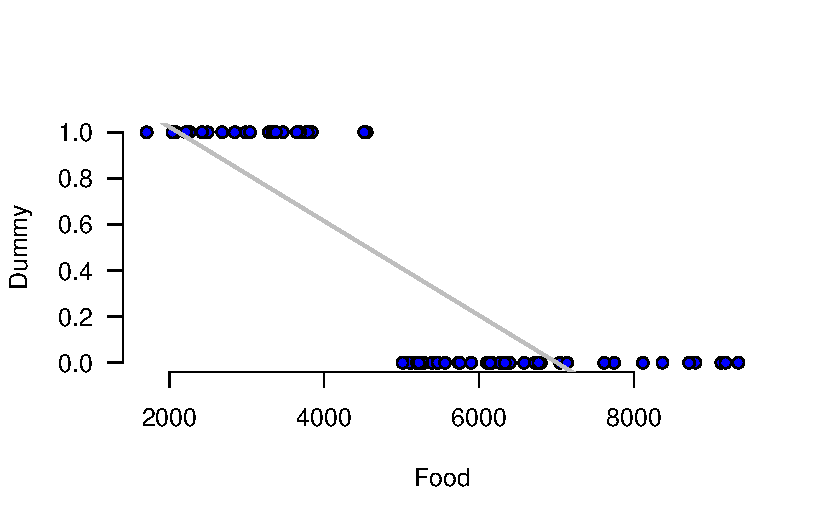
\includegraphics{./08-RegressionII_files/figure-pdf/unnamed-chunk-23-1.pdf}

}

\end{figure}

\hypertarget{exercise-4-3}{%
\subsection*{Exercise 4}\label{exercise-4-3}}
\addcontentsline{toc}{subsection}{Exercise 4}

\begin{blackbox}

\begin{enumerate}
\def\labelenumi{\arabic{enumi}.}
\tightlist
\item
  If we follow the \(R^2=0.81\) the model fits the data very well.
\end{enumerate}

\end{blackbox}

Let's load the data from the web:

\begin{Shaded}
\begin{Highlighting}[numbers=left,,]
\NormalTok{Population}\OtherTok{\textless{}{-}}\FunctionTok{read.csv}\NormalTok{(}\StringTok{"https://jagelves.github.io/Data/Population.csv"}\NormalTok{)}
\end{Highlighting}
\end{Shaded}

Now let's filter the data so that we can focus on the population for
Japan.

\begin{Shaded}
\begin{Highlighting}[numbers=left,,]
\FunctionTok{library}\NormalTok{(dplyr)}
\end{Highlighting}
\end{Shaded}

\begin{verbatim}

Attaching package: 'dplyr'
\end{verbatim}

\begin{verbatim}
The following objects are masked from 'package:stats':

    filter, lag
\end{verbatim}

\begin{verbatim}
The following objects are masked from 'package:base':

    intersect, setdiff, setequal, union
\end{verbatim}

\begin{Shaded}
\begin{Highlighting}[numbers=left,,]
\NormalTok{Japan}\OtherTok{\textless{}{-}}\FunctionTok{filter}\NormalTok{(Population,Country.Name}\SpecialCharTok{==}\StringTok{"Japan"}\NormalTok{)}
\end{Highlighting}
\end{Shaded}

Next, we can run the regression of \emph{Population} against the
\emph{Year}. Let's also run the \texttt{summary()} function to obtain
the fit and the coefficients.

\begin{Shaded}
\begin{Highlighting}[numbers=left,,]
\NormalTok{fit}\OtherTok{\textless{}{-}}\FunctionTok{lm}\NormalTok{(Population}\SpecialCharTok{\textasciitilde{}}\NormalTok{Year,}\AttributeTok{data=}\NormalTok{Japan)}
\FunctionTok{summary}\NormalTok{(fit)}
\end{Highlighting}
\end{Shaded}

\begin{verbatim}

Call:
lm(formula = Population ~ Year, data = Japan)

Residuals:
     Min       1Q   Median       3Q      Max 
-9583497 -4625571  1214644  4376784  5706004 

Coefficients:
              Estimate Std. Error t value Pr(>|t|)    
(Intercept) -988297581   68811582  -14.36   <2e-16 ***
Year            555944      34569   16.08   <2e-16 ***
---
Signif. codes:  0 '***' 0.001 '**' 0.01 '*' 0.05 '.' 0.1 ' ' 1

Residual standard error: 4871000 on 60 degrees of freedom
Multiple R-squared:  0.8117,    Adjusted R-squared:  0.8086 
F-statistic: 258.6 on 1 and 60 DF,  p-value: < 2.2e-16
\end{verbatim}

\begin{blackbox}

\begin{enumerate}
\def\labelenumi{\arabic{enumi}.}
\setcounter{enumi}{1}
\tightlist
\item
  The prediction for \(2030\) is about \(140\) million people.
\end{enumerate}

\end{blackbox}

Let's use the \texttt{predict()} function:

\begin{Shaded}
\begin{Highlighting}[numbers=left,,]
\FunctionTok{predict}\NormalTok{(fit,}\AttributeTok{newdata=}\FunctionTok{data.frame}\NormalTok{(}\AttributeTok{Year=}\FunctionTok{c}\NormalTok{(}\DecValTok{2030}\NormalTok{)))}
\end{Highlighting}
\end{Shaded}

\begin{verbatim}
        1 
140268585 
\end{verbatim}

\begin{blackbox}

\begin{enumerate}
\def\labelenumi{\arabic{enumi}.}
\setcounter{enumi}{2}
\tightlist
\item
  After looking at the scatter plot, it seems unlikely that the
  population in Japan will hit \(140\) million. Population has been
  decreasing in Japan!
\end{enumerate}

\end{blackbox}

Use the \texttt{plot()} and \texttt{abline()} functions to create the
figure.

\begin{Shaded}
\begin{Highlighting}[numbers=left,,]
\FunctionTok{plot}\NormalTok{(}\AttributeTok{y=}\NormalTok{Japan}\SpecialCharTok{$}\NormalTok{Population,}\AttributeTok{x=}\NormalTok{Japan}\SpecialCharTok{$}\NormalTok{Year, }\AttributeTok{main=}\StringTok{""}\NormalTok{, }
     \AttributeTok{axes=}\NormalTok{F,}\AttributeTok{pch=}\DecValTok{21}\NormalTok{, }\AttributeTok{bg=}\StringTok{"\#A7C7E7"}\NormalTok{,}
     \AttributeTok{xlab=}\StringTok{"Year"}\NormalTok{,}
     \AttributeTok{ylab=}\StringTok{"Population"}\NormalTok{)}
\FunctionTok{axis}\NormalTok{(}\AttributeTok{side=}\DecValTok{1}\NormalTok{, }\AttributeTok{labels=}\ConstantTok{TRUE}\NormalTok{, }\AttributeTok{font=}\DecValTok{1}\NormalTok{,}\AttributeTok{las=}\DecValTok{1}\NormalTok{)}
\FunctionTok{axis}\NormalTok{(}\AttributeTok{side=}\DecValTok{2}\NormalTok{, }\AttributeTok{labels=}\ConstantTok{TRUE}\NormalTok{, }\AttributeTok{font=}\DecValTok{1}\NormalTok{,}\AttributeTok{las=}\DecValTok{1}\NormalTok{)}
\FunctionTok{abline}\NormalTok{(fit,}
       \AttributeTok{col=}\StringTok{"darkgray"}\NormalTok{,}\AttributeTok{lwd=}\DecValTok{2}\NormalTok{)}
\end{Highlighting}
\end{Shaded}

\begin{figure}[H]

{\centering 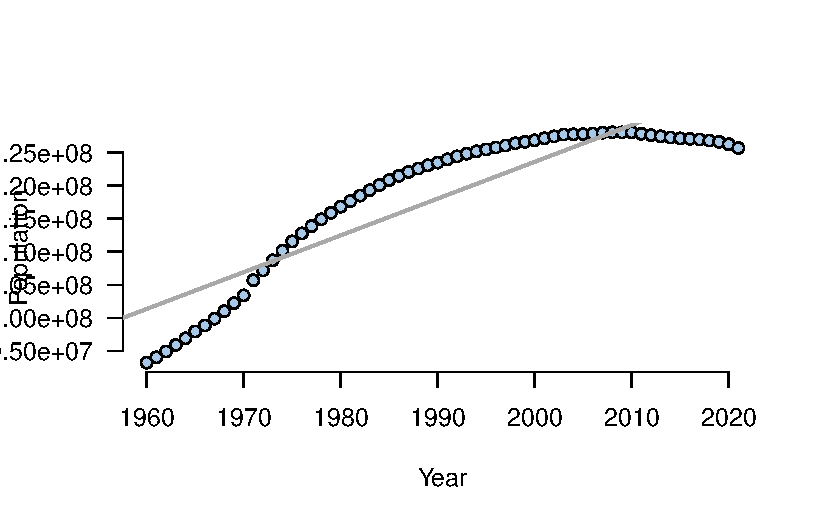
\includegraphics{./08-RegressionII_files/figure-pdf/unnamed-chunk-28-1.pdf}

}

\end{figure}

\part{Probability}

\hypertarget{probability-i}{%
\chapter{Probability I}\label{probability-i}}

\hypertarget{concepts-7}{%
\section{Concepts}\label{concepts-7}}

\hypertarget{experiments-and-sets}{%
\subsection*{Experiments and Sets}\label{experiments-and-sets}}
\addcontentsline{toc}{subsection}{Experiments and Sets}

An \textbf{experiment} is a process that leads to one of several
outcomes. Ex: Tossing a Die, Tossing a Coin, Drawing a Card, etc.

The \textbf{sample space} \((S)\) of an experiment contains all possible
outcomes of the experiment. Ex:
\(S\)=\{\(1\),\(2\),\(3\),\(4\),\(5\),\(6\)\} is the sample space for
tossing a die.

An \textbf{event} is a subset of the sample space. \(A\)=\{\(4\)\} is
the event of tossing a \(4\) when rolling a die.

\hypertarget{basic-probability-concepts}{%
\subsection*{Basic Probability
Concepts}\label{basic-probability-concepts}}
\addcontentsline{toc}{subsection}{Basic Probability Concepts}

A \textbf{probability} is a numerical value that measures the likelihood
that an event occurs.

To calculate \textbf{probabilities}, find the ratio between favorable
outcomes and total outcomes. \(p=favorable/total\).

\begin{itemize}
\item
  The probability of any event \(A\) is a value between \(0\) and \(1\)
  inclusive. Formally, \(0\leq P(A) \leq1\).
\item
  When the probability of the event is \(0\) then the event is
  impossible. When the probability is \(1\) then the event is certain.
\item
  The sum of the probabilities of a list of \textbf{mutually exclusive}
  and \textbf{exhaustive} events equals \(1\). Formally,
  \(\sum P(x_i)=1\).

  \begin{itemize}
  \item
    \textbf{Mutually exclusive} events do not share any common outcomes.
    The occurrence of one event precludes the occurrence of others.
  \item
    \textbf{Exhaustive} events include all outcomes in the sample space.
  \end{itemize}
\end{itemize}

To assign probabilities you can use the Empirical, Classical, or
Subjective Methods.

\begin{itemize}
\item
  Empirical: calculated as a relative frequency of occurrence.
\item
  Classical: based on logical analysis.
\item
  Subjective: calculated by drawing on personal and subjective
  judgement.
\end{itemize}

\hypertarget{probability-rules}{%
\subsection*{Probability Rules}\label{probability-rules}}
\addcontentsline{toc}{subsection}{Probability Rules}

The \textbf{Complement Rule}: \(P(A^c)=1-P(A)\), where \(A^c\) is the
complement of \(A\).

The \textbf{Addition Rule}: \(P(A \cup B)=P(A)+P(B)-P(A \cap B)\), where
\(\cap\) is intersection and \(\cup\) is union.

The \textbf{Multiplication Rule}:

\begin{itemize}
\item
  if events are dependent \(P(A \cap B)= P(A|B)P(B)\), where \(P(A|B)\)
  is the conditional probability.
\item
  if events are independent \(P(A \cap B)= P(A)P(B)\).
\end{itemize}

The \textbf{Law of Total Probability}:
\(P(A)=P(A|B)P(B)+P(A|B^c)P(B^c)\).

\textbf{Bayes' Theorem}: \(P(A|B)=P(B|A)P(A)/P(B)\).

\hypertarget{counting-rules}{%
\subsection*{Counting Rules}\label{counting-rules}}
\addcontentsline{toc}{subsection}{Counting Rules}

The \textbf{Combination} function counts the number of ways to choose
\(x\) objects from a total of \(n\) objects. The order in which the
\(x\) objects are listed does not matter.

\begin{itemize}
\item
  If repetition is not allowed use \(C_n^x= \frac{n!}{(n-x)!x!}\).
\item
  If repetition is allowed use \(\frac{(x+n-1)!}{(n-x)!x!}\).
\end{itemize}

The \textbf{Permutation} function also counts the number of ways to
choose \(x\) objects from a total of \(n\) objects. However, the order
in which the \(x\) objects are listed does matter.

\begin{itemize}
\item
  If repetition is not allowed use \(P_n^x= \frac{n!}{(n-x)!}\).
\item
  If repetition is allowed use \(n^x\).
\end{itemize}

\hypertarget{useful-r-functions-7}{%
\subsection*{Useful R Functions}\label{useful-r-functions-7}}
\addcontentsline{toc}{subsection}{Useful R Functions}

The \texttt{table()} function can be used to construct frequency
distributions.

The \texttt{factorial()} function returns the factorial of a number.

The \texttt{gtools} package contains the \texttt{combinations()} and
\texttt{permutations()} functions used to calculate combinations and
permutations. Use the \emph{repeats.allowed} argument to specify
counting with repetition or no repetition.

\hypertarget{exercises-7}{%
\section{Exercises}\label{exercises-7}}

The following exercises will help you practice some probability concepts
and formulas. In particular, the exercises work on:

\begin{itemize}
\item
  Calculating simple probabilities.
\item
  Applying probability rules.
\item
  Using counting rules.
\end{itemize}

Answers are provided below. Try not to peak until you have a formulated
your own answer and double checked your work for any mistakes.

\hypertarget{exercise-1-14}{%
\subsection*{Exercise 1}\label{exercise-1-14}}
\addcontentsline{toc}{subsection}{Exercise 1}

For the following exercises, make your calculations by hand and verify
results with a calculator or R.

\begin{enumerate}
\def\labelenumi{\arabic{enumi}.}
\item
  A sample space \(S\) yields five equally likely events, \(A\), \(B\),
  \(C\), \(D\), and \(E\). Find \(P(D)\), \(P(B^c)\), and
  \(P(A \cup C \cup E)\).
\item
  Consider the roll of a die. Define \(A\) as \{1,2,3\}, \(B\) as
  \{1,2,3,5,6\}, \(C\) as \{4,6\}, and \(D\) as \{4,5,6\}. Are the
  events \(A\) and \(B\) mutually exclusive, exhaustive, both or none?
  What about events \(A\) and \(D\)?
\item
  A recent study suggests that \(33.1\)\% of the adult U.S. population
  is overweight and \(35.7\)\% obese. What is the probability that a
  randomly selected adult in the U.S. is either obese or overweight?
  What is the probability that their weight is normal? Are the events
  mutually exclusive and exhaustive?
\end{enumerate}

\hypertarget{exercise-2-14}{%
\subsection*{Exercise 2}\label{exercise-2-14}}
\addcontentsline{toc}{subsection}{Exercise 2}

For the following exercises, make your calculations by hand and verify
results with a calculator or R.

\begin{enumerate}
\def\labelenumi{\arabic{enumi}.}
\item
  Let \(P(A)=0.65\), \(P(B)=0.3\), and \(P(A|B)=0.45\). Calculate
  \(P(A \cap B)\), \(P(A \cup B)\), and \(P(B|A)\).
\item
  Let \(P(A)=0.4\), \(P(B)=0.5\), and \(P(A^c \cap B^c)=0.24\).
  Calculate \(P(A^c|B^c)=0.24\), \(P(A^c \cup B^c)\), and
  \(P(A \cup B)\).
\item
  Stock \(A\) will rise in price with a probability of \(0.4\), stock
  \(B\) will rise with a probability of \(0.6\). If stock \(B\) rises in
  price, then \(A\) will also rise with a probability of \(0.5\). What
  is the probability that at least one of the stocks will rise in price?
  Prove that events \(A\) and \(B\) are (are not) mutually exclusive
  (independent).
\end{enumerate}

\hypertarget{exercise-3-14}{%
\subsection*{Exercise 3}\label{exercise-3-14}}
\addcontentsline{toc}{subsection}{Exercise 3}

\begin{enumerate}
\def\labelenumi{\arabic{enumi}.}
\tightlist
\item
  Create a joint probability table from the contingency table below.
  Find \(P(A)\), \(P(A \cap B)\), \(P(A|B)\), and \(P(B|A^c)\).
  Determine whether the events are independent or mutually exclusive.
\end{enumerate}

\begin{longtable}[]{@{}lll@{}}
\toprule()
\endhead
& \(A^c\) & \(B^c\) \\
\(A\) & 26 & 34 \\
\(B\) & 14 & 26 \\
\bottomrule()
\end{longtable}

\hypertarget{exercise-4-4}{%
\subsection*{Exercise 4}\label{exercise-4-4}}
\addcontentsline{toc}{subsection}{Exercise 4}

You will need the \textbf{Crash} data set and R to answer this question.
The data shows information on several car crashes. Specifically, if the
crash was Head-On or Not Head-On and whether there was Daylight or No
Daylight.

\begin{enumerate}
\def\labelenumi{\arabic{enumi}.}
\item
  Create a contingency table.
\item
  Find the probability that a) a car crash is Head-On, b) a car crash is
  in daylight c) a car crash is Head-On given that there is daylight.
\item
  Show that Crashes and Light are dependent.
\end{enumerate}

\hypertarget{exercise-5}{%
\subsection*{Exercise 5}\label{exercise-5}}
\addcontentsline{toc}{subsection}{Exercise 5}

\begin{enumerate}
\def\labelenumi{\arabic{enumi}.}
\item
  Use Bayes' Theorem in the following question. Let \(P(A)=0.7\),
  \(P(B|A)=0.55\), and \(P(B|A^c)=0.10\). Find \(P(A^c)\),
  \(P(A \cap B)\), \(P(A^c \cap B)\), \(P(B)\), and \(P(A|B)\).
\item
  Some find tutors helpful when taking a course. Julia has a 40\% chance
  to fail a course if she does not have a tutor. With a tutor, the
  probability of failing is only 10\%. There is a 50\% chance that Julia
  finds an available tutor. What is the probability that Julia will fail
  the course? If she ends up failing the course, what is the probability
  that she had a tutor?
\end{enumerate}

\hypertarget{exercise-6}{%
\subsection*{Exercise 6}\label{exercise-6}}
\addcontentsline{toc}{subsection}{Exercise 6}

\begin{enumerate}
\def\labelenumi{\arabic{enumi}.}
\item
  Calculate the following values and verify your results using R. a) 3!,
  b) 4!, c) \(C_6^8\), d) \(P_6^8\).
\item
  There are 10 players in a local basketball team. If we chose 5 players
  to randomly start a game, in how many ways can we select the five
  players if order doesn't matter? What if order matters?
\end{enumerate}

\hypertarget{answers-7}{%
\section{Answers}\label{answers-7}}

\hypertarget{exercise-1-15}{%
\subsection*{Exercise 1}\label{exercise-1-15}}
\addcontentsline{toc}{subsection}{Exercise 1}

\begin{blackbox}

\begin{enumerate}
\def\labelenumi{\arabic{enumi}.}
\tightlist
\item
  \(P(D)=1/5=0.2\) since all events are equally likely.
  \(P(B^c)=4/5=0.8\), and \(P(A \cup C \cup E)=P(A + C + E)=3/5=0.6\).
\end{enumerate}

\end{blackbox}

\begin{blackbox}

\begin{enumerate}
\def\labelenumi{\arabic{enumi}.}
\setcounter{enumi}{1}
\tightlist
\item
  Events \(A\) and \(B\) are not mutually exclusive since they share
  some of the same elements. They are not exhaustive since the union of
  both doesn't create the sample space.
\end{enumerate}

\end{blackbox}

\begin{blackbox}

\begin{enumerate}
\def\labelenumi{\arabic{enumi}.}
\setcounter{enumi}{2}
\tightlist
\item
  The probability is \(68.8\)\%. The events are mutually exclusive. If
  someone is classified as obese, the person is not classified again as
  overweight. The events are not exhaustive since there are people in
  the U.S. that have a normal weight. The probability that the person
  drawn has normal weight is \(31.2\)\%.
\end{enumerate}

\end{blackbox}

\hypertarget{exercise-2-15}{%
\subsection*{Exercise 2}\label{exercise-2-15}}
\addcontentsline{toc}{subsection}{Exercise 2}

\begin{blackbox}

\begin{enumerate}
\def\labelenumi{\arabic{enumi}.}
\tightlist
\item
  From the multiplication rule, \(P(A|B)*P(B)=P(A \cap B)\).\\
  Substituting values yields, \(P(A \cap B)=0.45*0.3=0.135\).\\
  From the addition rule, \(P(A \cup B)=P(A)+P(B)-P(A \cap B)\).\\
  Substituting yields, \(P(A \cup B)=0.65+0.3-0.135=0.815\).\\
  From the multiplication rule once again,
  \(P(B|A)=\frac{P(A \cap B)}{P(A)}\). Substituting yields,
  \(P(B|A)=0.135/0.65=0.2076923\).
\end{enumerate}

\end{blackbox}

\begin{blackbox}

\begin{enumerate}
\def\labelenumi{\arabic{enumi}.}
\setcounter{enumi}{1}
\tightlist
\item
  From the complement rule we have that \(P(A^c)=0.6\) and
  \(P(B^c)=0.5\).\\
  Using the multiplication rule,
  \(P(A^c|B^c)=\frac{P(A^c \cap B^c)}{P(B^c)}\). Substituting yields
  \(P(A^c|B^c)=0.24/0.5=0.48\).\\
  From the addition rule
  \(P(A^c \cup B^c)=P(A^c)+P(B^c)-P(A^c \cap B^c)\).\\
  Substituting yields \(P(A^c \cup B^c)=0.6+0.5-0.24=0.86\).\\
  The event that has no elements of \(A\) or \(B\) is given by
  \(P(A^c \cap B^c)\). Therefore \(P(A \cup B)=1-0.24=0.76\) has all the
  elements of A and B.
\end{enumerate}

\end{blackbox}

\begin{blackbox}

\begin{enumerate}
\def\labelenumi{\arabic{enumi}.}
\setcounter{enumi}{2}
\tightlist
\item
  In short the problem states \(P(A)=0.4\), \(P(B)=0.6\), and
  \(P(A|B)=0.5\). Where \(A\) and \(B\) are events of stocks rising in
  price. The question asks for \(P(A \cup B)=P(A)+P(B)-P(A \cap B)\).\\
  Using the multiplication rule \(P(A \cap B)=0.5*0.6=0.3\).\\
  Hence, \(P(A \cup B)=0.4+0.6-0.3=0.7\).\\
  The events are not mutually exclusive since
  \(P(A \cap B)=0.3 \neq 0\).\\
  The events are also not independent since
  \(P(A|B)=0.5 \neq 0.4=P(A)\).
\end{enumerate}

\end{blackbox}

\hypertarget{exercise-3-15}{%
\subsection*{Exercise 3}\label{exercise-3-15}}
\addcontentsline{toc}{subsection}{Exercise 3}

\begin{blackbox}

\begin{enumerate}
\def\labelenumi{\arabic{enumi}.}
\tightlist
\item
  Below is the joint probability table. The \(P(A)=0.26+0.34=0.6\),
  \(P(A \cap B)=0.26\), \(P(A|B)=0.26/0.4=0.65\), and
  \(P(B|A^c)=0.14/0.4=0.35\). Events \(A\) and \(B\) are not independent
  since \(P(A) \neq P(A|B)\). The events are not mutually exclusive
  since \(P(A \cap B)=0.26 \neq 0\).
\end{enumerate}

\end{blackbox}

\begin{longtable}[]{@{}llll@{}}
\toprule()
\endhead
& \(B\) & \(B^c\) & Total \\
\(A\) & 0.26 & 0.34 & 0.6 \\
\(A^c\) & 0.14 & 0.26 & 0.4 \\
Total & 0.4 & 0.6 & 1 \\
\bottomrule()
\end{longtable}

\hypertarget{exercise-4-5}{%
\subsection*{Exercise 4}\label{exercise-4-5}}
\addcontentsline{toc}{subsection}{Exercise 4}

\begin{blackbox}

\begin{enumerate}
\def\labelenumi{\arabic{enumi}.}
\tightlist
\item
  The probability of a Head-On crash is \((166+108)/4858=0.056\). The
  probability of a daylight crash is \((166+3258)/4858=0.70\). The
  probability that the car crash is Head-On given daylight is
  \(166/(166+3258)=0.048\).
\end{enumerate}

\end{blackbox}

Start by loading the data into R.

\begin{Shaded}
\begin{Highlighting}[numbers=left,,]
\NormalTok{Crash}\OtherTok{\textless{}{-}}\FunctionTok{read.csv}\NormalTok{(}\StringTok{"https://jagelves.github.io/Data/Crash.csv"}\NormalTok{)}
\end{Highlighting}
\end{Shaded}

To create a contingency table use the \texttt{table()} command in R.

\begin{Shaded}
\begin{Highlighting}[numbers=left,,]
\FunctionTok{table}\NormalTok{(Crash}\SpecialCharTok{$}\StringTok{\textasciigrave{}}\AttributeTok{Crash Type}\StringTok{\textasciigrave{}}\NormalTok{,Crash}\SpecialCharTok{$}\StringTok{\textasciigrave{}}\AttributeTok{Light Condition}\StringTok{\textasciigrave{}}\NormalTok{)}
\end{Highlighting}
\end{Shaded}

\begin{verbatim}
< table of extent 0 x 0 >
\end{verbatim}

This table is used to calculate probabilities.

\begin{blackbox}

\begin{enumerate}
\def\labelenumi{\arabic{enumi}.}
\setcounter{enumi}{1}
\tightlist
\item
  The two variables are dependent since
  \(P(Head-On|Daylight) \neq P(Head-On)\), that is \(0.048 \neq 0.56\).
\end{enumerate}

\end{blackbox}

\hypertarget{exercise-5-1}{%
\subsection*{Exercise 5}\label{exercise-5-1}}
\addcontentsline{toc}{subsection}{Exercise 5}

\begin{blackbox}

\begin{enumerate}
\def\labelenumi{\arabic{enumi}.}
\tightlist
\item
  \(P(A^c)=1-P(A)=1-0.7=0.3\),
  \(P(A \cap B)=𝑃(𝐵|𝐴)𝑃(𝐴) = 0.55(0.70) = 0.385\),
  \(P(A^c \cap B)=𝑃(B|A^c)𝑃(A^c) = 0.10(0.30) = 0.03\),
  \(P(B)= 𝑃(A \cap B) + 𝑃(𝐴^c \cap 𝐵) = 0.385 + 0.03 = 0.415\), and
  \(P(A|B)= \frac{𝑃(A \cap B)}{P(B)}=0.385/0.415=0.9277\).
\end{enumerate}

\end{blackbox}

\begin{blackbox}

\begin{enumerate}
\def\labelenumi{\arabic{enumi}.}
\setcounter{enumi}{1}
\tightlist
\item
  Let the event of failing be \(F\), the event of not failing be \(NF\),
  the event of having a tutor be \(T\), and the event of not having a
  tutor be \(NT\). The probability of failing the course is \(0.25\).
  \((𝐹) = 𝑃(𝐹 \cap 𝑇) + 𝑃(𝐹 \cap 𝑇^c) = 𝑃(𝐹|𝑇)𝑃(𝑇) + 𝑃(𝐹|𝑇^c)𝑃(𝑇^c) = 0.10(0.50) + 0.40(0.50) = 0.05 + 0.20 = 0.25\)
  The probability of not having a tutor, given that she failed the
  course is \(0.2\).
  \(P(𝑇|𝐹) = \frac{𝑃(𝐹\cap𝑇)}{𝑃(𝐹\cap𝑇)+𝑃(𝐹 \cap𝑇^c)}= 0.05/0.25 = 0.20\)
\end{enumerate}

\end{blackbox}

\hypertarget{exercise-6-1}{%
\subsection*{Exercise 6}\label{exercise-6-1}}
\addcontentsline{toc}{subsection}{Exercise 6}

\begin{blackbox}

\begin{enumerate}
\def\labelenumi{\arabic{enumi}.}
\tightlist
\item
  \(3!=3 \times 2 \times 1=6\), \(4!=6 \times 4=24\), \(C_6^8=28\), and
  \(P_6^8=20,160\)
\end{enumerate}

\end{blackbox}

In R we can just use the factorial command. So \(3!\) is:

\begin{Shaded}
\begin{Highlighting}[numbers=left,,]
\FunctionTok{factorial}\NormalTok{(}\DecValTok{3}\NormalTok{)}
\end{Highlighting}
\end{Shaded}

\begin{verbatim}
[1] 6
\end{verbatim}

and \(4!\) is:

\begin{Shaded}
\begin{Highlighting}[numbers=left,,]
\FunctionTok{factorial}\NormalTok{(}\DecValTok{4}\NormalTok{)}
\end{Highlighting}
\end{Shaded}

\begin{verbatim}
[1] 24
\end{verbatim}

For combinations and permutations we can use the \texttt{gtools}
package:

\begin{Shaded}
\begin{Highlighting}[numbers=left,,]
\FunctionTok{library}\NormalTok{(gtools)}
\NormalTok{C}\OtherTok{\textless{}{-}}\FunctionTok{combinations}\NormalTok{(}\DecValTok{8}\NormalTok{,}\DecValTok{6}\NormalTok{)}
\FunctionTok{nrow}\NormalTok{(C)}
\end{Highlighting}
\end{Shaded}

\begin{verbatim}
[1] 28
\end{verbatim}

\begin{Shaded}
\begin{Highlighting}[numbers=left,,]
\FunctionTok{library}\NormalTok{(gtools)}
\NormalTok{P}\OtherTok{\textless{}{-}}\FunctionTok{permutations}\NormalTok{(}\DecValTok{8}\NormalTok{,}\DecValTok{6}\NormalTok{)}
\FunctionTok{nrow}\NormalTok{(P)}
\end{Highlighting}
\end{Shaded}

\begin{verbatim}
[1] 20160
\end{verbatim}

\begin{blackbox}

\begin{enumerate}
\def\labelenumi{\arabic{enumi}.}
\setcounter{enumi}{1}
\tightlist
\item
  If order doesn't matter, there are \(252\) ways. If order matters,
  then there are \(30,240\) ways.
\end{enumerate}

\end{blackbox}

In R we can once more use the combination and permutation functions:

\begin{Shaded}
\begin{Highlighting}[numbers=left,,]
\NormalTok{B1}\OtherTok{\textless{}{-}}\FunctionTok{combinations}\NormalTok{(}\DecValTok{10}\NormalTok{,}\DecValTok{5}\NormalTok{)}
\FunctionTok{nrow}\NormalTok{(B1)}
\end{Highlighting}
\end{Shaded}

\begin{verbatim}
[1] 252
\end{verbatim}

\begin{Shaded}
\begin{Highlighting}[numbers=left,,]
\NormalTok{B2}\OtherTok{\textless{}{-}}\FunctionTok{permutations}\NormalTok{(}\DecValTok{10}\NormalTok{,}\DecValTok{5}\NormalTok{)}
\FunctionTok{nrow}\NormalTok{(B2)}
\end{Highlighting}
\end{Shaded}

\begin{verbatim}
[1] 30240
\end{verbatim}

\hypertarget{probability-ii}{%
\chapter{Probability II}\label{probability-ii}}

\hypertarget{concepts-8}{%
\section{Concepts}\label{concepts-8}}

\hypertarget{random-variables}{%
\subsection*{Random Variables}\label{random-variables}}
\addcontentsline{toc}{subsection}{Random Variables}

A \textbf{random variable} associates a numerical value with each
possible experimental outcome. Specifically, the random variable takes
on a value with some probability.

A random variable is fully characterized by its \textbf{probability
density function} (PDF) if continuous or the \textbf{probability mass
function} (PMF) if discrete.

\hypertarget{expected-value-and-variance}{%
\subsection*{Expected Value and
Variance}\label{expected-value-and-variance}}
\addcontentsline{toc}{subsection}{Expected Value and Variance}

When summarizing a random variable, we are mostly interested in the
variable's central tendency (Expected Value) and dispersion (Variance).

The \textbf{expected value} (mean) is a measure of central location. For
a discrete random variable it is given by \(E(x)=\mu=\sum xf(x)\), where
\(f(x)\) is the probability mass function. For a continuous random
variable it is given by \(E(x)= \int_{-\infty}^{\infty} x f(x) dx\),
where \(f(x)\) is the probability density function.

The \textbf{variance} summarizes the deviation of the values of the
random variable from the mean. It is calculated by
\(var(x)=E[(x-E(x))^2]=E[x^2]-E[x]^2\). Note that this formula can be
used for both discrete and continuous random variables.

\hypertarget{discrete-uniform-distribution}{%
\subsection*{Discrete Uniform
Distribution}\label{discrete-uniform-distribution}}
\addcontentsline{toc}{subsection}{Discrete Uniform Distribution}

The \textbf{discrete uniform distribution} is a probability distribution
that assigns equal probability to each outcome in a finite set of
possible outcomes. In other words, each outcome in the set is equally
likely to occur.

The \textbf{probability mass function} is given by \(f(x)=1/n\), where
\(n\) is the number of elements in the sample space (all possible
outcomes).

The \textbf{expected value} is given by \(E(x)=\frac {a+b}{2}\), where
\(a\) is the lower bound of the distribution, and \(b\) is the upper
bound.

The \textbf{variance} is given by \(var(x)=\frac {(n^2-1)}{12}\).

\hypertarget{binomial-distribution}{%
\subsection*{Binomial Distribution}\label{binomial-distribution}}
\addcontentsline{toc}{subsection}{Binomial Distribution}

The binomial distribution is a probability distribution that describes
the outcome of a sequence of \(n\) independent Bernoulli trials. In a
Bernoulli trial, there are only two possible outcomes: ``success'' and
``failure''. The probability of success is denoted by \(p\), and the
probability of failure is denoted by \(q = 1 - p\). In a sequence of
\(n\) independent Bernoulli trials, the number of successes (\(x\)) is a
random variable that follows a binomial distribution.

The \textbf{probability mass function} is given by
\(f(x)=C_x^n (p^x)(1-p)^{n-x}\), where \(n\) is the number of trials,
\(x\) is the number of successes, \(p\) is the probability of success,
and \(C_x^n\) is the number of ways there can be \(x\) successes in
\(n\) trials.

The \textbf{expected value} of the binomial distribution is \(E(x)=np\).

The \textbf{variance} of the binomial distribution is
\(var(x)=np(1-p)\).

\hypertarget{the-hypergeometric-distribution}{%
\subsection*{The Hypergeometric
Distribution}\label{the-hypergeometric-distribution}}
\addcontentsline{toc}{subsection}{The Hypergeometric Distribution}

The \textbf{hypergeometric distribution} is a probability distribution
that describes the outcome of drawing a sample from a population without
replacement. It is used to calculate the probability of drawing a
certain number of successes (\(x\)) in a sample of a given size (\(n\)),
where the success or failure of each individual draw is not dependent on
the success or failure of other draws.

The \textbf{hypergeometric} experiment differs from the binomial since:

\begin{itemize}
\item
  trials are not independent.
\item
  the probability of success changes from trial to trial.
\end{itemize}

The \textbf{probability mass function} is given by
\(f(x)=\frac {C_x^r C_{n-x}^{N-r}}{C_n^N}\), where \(n\) is the number
of trials, \(x\) is the number of successes, \(r\) is the number of
elements in the population labeled as success, and \(N\) is the number
of elements in the population.

The \textbf{expected value} of the hypergeometric distribution is
\(E(x)=n \frac {r}{N}\).

The \textbf{variance} of the hypergeometric distribution is
\(var(x)= n \frac {r}{N} (1- \frac {r}{N}) (\frac {N-n}{N-1})\).

\hypertarget{poisson-distribution}{%
\subsection*{Poisson Distribution}\label{poisson-distribution}}
\addcontentsline{toc}{subsection}{Poisson Distribution}

The \textbf{Poisson distribution} estimates the number of successes
(\(x\)) over a specified interval of time or space.

The \textbf{probability mass function} is given by
\(f(x)= \frac {\mu e^{-x}}{x!}\), where \(\mu\) is the expected number
of successes in any given interval and also the variance, and \(e\) is
Euler's number (2.71828\ldots).

An experiment satisfies a Poisson process if:

\begin{itemize}
\item
  The number of successes with a specified time or space interval equals
  any integer between zero and infinity.
\item
  The number of successes counted in non-overlapping intervals are
  independent.
\item
  The probability of success in any interval is the same for all
  intervals of equal size and is proportional to the size of the
  interval.
\end{itemize}

\hypertarget{useful-r-functions-8}{%
\subsection*{Useful R Functions}\label{useful-r-functions-8}}
\addcontentsline{toc}{subsection}{Useful R Functions}

To calculate probabilities based on discrete random variables use the
\texttt{pbinom()}, \texttt{phyper()}, and \texttt{ppois()} functions.
For the uniform distribution use the \texttt{extraDistr} package and the
\texttt{pdunif()} function.

To calculate cumulative probabilities use the \texttt{dbinom()},
\texttt{dhyper()}, \texttt{dpois()}, and \texttt{ddunif()} functions.

To calculate quantiles use the \texttt{qbinom()}, \texttt{qhyper()},
\texttt{qpois()}, and \texttt{qdunif()} functions.

To generate random numbers use the \texttt{rbinom()}, \texttt{rhyper()},
\texttt{rpois()}, and \texttt{rdunif()} functions.

\hypertarget{exercises-8}{%
\section{Exercises}\label{exercises-8}}

The following exercises will help you practice some probability concepts
and formulas. In particular, the exercises work on:

\begin{itemize}
\item
  Calculating probabilities for discrete random variables.
\item
  Calculating the expected value and standard deviation.
\item
  Applying the binomial, Poisson and hypergeometric probability
  distributions.
\end{itemize}

Answers are provided below. Try not to peak until you have a formulated
your own answer and double checked your work for any mistakes.

\hypertarget{exercise-1-16}{%
\subsection*{Exercise 1}\label{exercise-1-16}}
\addcontentsline{toc}{subsection}{Exercise 1}

For the following exercises, make your calculations by hand and verify
results with a calculator or R.

\begin{enumerate}
\def\labelenumi{\arabic{enumi}.}
\tightlist
\item
  Consider the table below. Calculate the mean and standard deviation.
  What is the probability that \(x<15\)?
\end{enumerate}

\begin{longtable}[]{@{}lllll@{}}
\toprule()
\endhead
\(x\) & 5 & 10 & 15 & 20 \\
\(P(X=x)\) & 0.35 & 0.3 & 0.2 & 0.15 \\
\bottomrule()
\end{longtable}

\begin{enumerate}
\def\labelenumi{\arabic{enumi}.}
\setcounter{enumi}{1}
\tightlist
\item
  Consider the table below. Calculate the mean and standard deviation.
  What is the probability that \(x\geq-9\)?
\end{enumerate}

\begin{longtable}[]{@{}lllll@{}}
\toprule()
\endhead
\(y\) & -23 & -17 & -9 & -3 \\
\(P(Y=y)\) & 0.5 & 0.25 & 0.15 & 0.1 \\
\bottomrule()
\end{longtable}

\begin{enumerate}
\def\labelenumi{\arabic{enumi}.}
\setcounter{enumi}{2}
\tightlist
\item
  The returns on a couple of funds depends on the state of the economy.
  The economy is expected to be Good with a probability of 20\%, Fair
  with probability of 50\% and Poor with probability of 30\%. Which fund
  would you choose if you want to maximize your return? What would you
  choose if you really dislike risk?
\end{enumerate}

\begin{longtable}[]{@{}ccc@{}}
\toprule()
State of Economy & Fund 1 & Fund 2 \\
\midrule()
\endhead
Good & 20 & 40 \\
Fair & 10 & 20 \\
Poor & -10 & -40 \\
\bottomrule()
\end{longtable}

\hypertarget{exercise-2-16}{%
\subsection*{Exercise 2}\label{exercise-2-16}}
\addcontentsline{toc}{subsection}{Exercise 2}

\begin{enumerate}
\def\labelenumi{\arabic{enumi}.}
\tightlist
\item
  Use the table below. A portfolio has 200,000 dollars invested in Asset
  \(X\) and 300,000 dollars in asset \(Y\). If the correlation
  coefficient between the two investments is \(0.4\), what is the
  expected return and standard deviation of the portfolio?
\end{enumerate}

\begin{longtable}[]{@{}ccc@{}}
\toprule()
Measure & X & Y \\
\midrule()
\endhead
Expected Return (\%) & 8 & 12 \\
Standard Deviation (\%) & 12 & 20 \\
\bottomrule()
\end{longtable}

\hypertarget{exercise-3-16}{%
\subsection*{Exercise 3}\label{exercise-3-16}}
\addcontentsline{toc}{subsection}{Exercise 3}

\begin{enumerate}
\def\labelenumi{\arabic{enumi}.}
\item
  Let \(Z\) be a binomial random variable with \(n=5\) and \(p=0.35\)
  use the binomial formula to find \(P(Z=1)\), \(P(Z \geq 2)\). What is
  the expected value and standard deviation of \(Z\)?
\item
  Let \(W\) be a binomial random variable with \(n=200\) and \(p=0.77\)
  use the binomial formula to find \(P(W>160)\),
  \(P(155 \leq W \leq 165)\). What is the expected value and standard
  deviation of \(W\)?
\item
  Sixty percent of a firm's employees are men. Suppose four of the
  firm's employees are randomly selected. What is more likely, finding
  three men and one woman, or two men and one woman? Does your answer
  change if the proportion falls to \(50\)\%?
\end{enumerate}

\hypertarget{exercise-4-6}{%
\subsection*{Exercise 4}\label{exercise-4-6}}
\addcontentsline{toc}{subsection}{Exercise 4}

\begin{enumerate}
\def\labelenumi{\arabic{enumi}.}
\item
  Assume that \(S\) is a Poisson process with mean of \(\mu=1.5\).
  Calculate \(P(S=2)\) and \(P(S \geq 2)\). What is the mean and
  standard deviation of \(S\)?
\item
  Assume that \(T\) is a Poisson process with mean of \(\mu=20\).
  Calculate \(P(T=14)\) and \(P(18 \leq T \leq 23)\).
\item
  A local pharmacy administers on average \(84\) Covid-19 vaccines per
  week. The vaccines shots are evenly administered across all days. Find
  the probability that the number of vaccine shots administered on a
  Wednesday is more than eight but less than \(12\).
\end{enumerate}

\hypertarget{exercise-5-2}{%
\subsection*{Exercise 5}\label{exercise-5-2}}
\addcontentsline{toc}{subsection}{Exercise 5}

\begin{enumerate}
\def\labelenumi{\arabic{enumi}.}
\item
  Assume that \(X\) is a hypergeometric random variable with \(N=25\),
  \(S=3\), and \(n=4\). Calculate \(P(X=0)\), \(P(X=1)\), and
  \(P(X \leq 1)\).
\item
  Compute the probability of at least eight successes in a random sample
  of \(20\) items obtained from a population of \(100\) items that
  contains \(25\) successes. What are the expected value and standard
  deviation of the number of successes?
\item
  For \(1\) dollar a player gets to select six numbers for the base game
  of Powerball. In the game, five balls are randomly drawn from 59
  consecutively numbered white balls. One ball, called the Powerball, is
  randomly drawn from \(39\) consecutively numbered red balls. What is
  the probability that a player is able to match two out of five
  randomly drawn white balls? What is the probability of winning the
  jackpot?
\end{enumerate}

\hypertarget{answers-8}{%
\section{Answers}\label{answers-8}}

\hypertarget{exercise-1-17}{%
\subsection*{Exercise 1}\label{exercise-1-17}}
\addcontentsline{toc}{subsection}{Exercise 1}

\begin{blackbox}

\begin{enumerate}
\def\labelenumi{\arabic{enumi}.}
\tightlist
\item
  The expected value is \(10.75\) and the standard deviation is
  \(5.31\). The probability of \(x<15\) is \(0.65\).
\end{enumerate}

\end{blackbox}

In R we can create vectors for both \(x\) and the probabilities
\(P(X=x)\).

\begin{Shaded}
\begin{Highlighting}[numbers=left,,]
\NormalTok{x}\OtherTok{\textless{}{-}}\FunctionTok{c}\NormalTok{(}\DecValTok{5}\NormalTok{,}\DecValTok{10}\NormalTok{,}\DecValTok{15}\NormalTok{,}\DecValTok{20}\NormalTok{)}
\NormalTok{px}\OtherTok{\textless{}{-}}\FunctionTok{c}\NormalTok{(}\FloatTok{0.35}\NormalTok{,}\FloatTok{0.3}\NormalTok{,}\FloatTok{0.2}\NormalTok{,}\FloatTok{0.15}\NormalTok{)}
\end{Highlighting}
\end{Shaded}

The expected value is the sum product of probabilities and values.
Formally, \(\sum_{i=1}^{n}x_{i}p_{i}\) and in R:

\begin{Shaded}
\begin{Highlighting}[numbers=left,,]
\NormalTok{(ex}\OtherTok{\textless{}{-}}\FunctionTok{sum}\NormalTok{(x}\SpecialCharTok{*}\NormalTok{px))}
\end{Highlighting}
\end{Shaded}

\begin{verbatim}
[1] 10.75
\end{verbatim}

The standard deviation is given by
\(\sqrt{\sum_{i=1}^{n}(x_{i}-\mu)^2p_{i}}\). We can calculate it in R
with the following code:

\begin{Shaded}
\begin{Highlighting}[numbers=left,,]
\NormalTok{(sd}\OtherTok{\textless{}{-}}\FunctionTok{sqrt}\NormalTok{(}\FunctionTok{sum}\NormalTok{((x}\SpecialCharTok{{-}}\NormalTok{ex)}\SpecialCharTok{\^{}}\DecValTok{2}\SpecialCharTok{*}\NormalTok{px)))}
\end{Highlighting}
\end{Shaded}

\begin{verbatim}
[1] 5.30919
\end{verbatim}

\begin{blackbox}

\begin{enumerate}
\def\labelenumi{\arabic{enumi}.}
\setcounter{enumi}{1}
\tightlist
\item
  The expected value is \(-17.4\) and the standard deviation is
  \(6.86\). The probability of is \(0.25\).
\end{enumerate}

\end{blackbox}

Let's create the vectors once more in R.

\begin{Shaded}
\begin{Highlighting}[numbers=left,,]
\NormalTok{y}\OtherTok{\textless{}{-}}\FunctionTok{c}\NormalTok{(}\SpecialCharTok{{-}}\DecValTok{23}\NormalTok{,}\SpecialCharTok{{-}}\DecValTok{17}\NormalTok{,}\SpecialCharTok{{-}}\DecValTok{9}\NormalTok{,}\SpecialCharTok{{-}}\DecValTok{3}\NormalTok{)}
\NormalTok{py}\OtherTok{\textless{}{-}}\FunctionTok{c}\NormalTok{(}\FloatTok{0.5}\NormalTok{,}\FloatTok{0.25}\NormalTok{,}\FloatTok{0.15}\NormalTok{,}\FloatTok{0.1}\NormalTok{)}
\end{Highlighting}
\end{Shaded}

The expected value is given by:

\begin{Shaded}
\begin{Highlighting}[numbers=left,,]
\NormalTok{(ey}\OtherTok{\textless{}{-}}\FunctionTok{sum}\NormalTok{(y}\SpecialCharTok{*}\NormalTok{py))}
\end{Highlighting}
\end{Shaded}

\begin{verbatim}
[1] -17.4
\end{verbatim}

The standard deviation is given by:

\begin{Shaded}
\begin{Highlighting}[numbers=left,,]
\NormalTok{(sdy}\OtherTok{\textless{}{-}}\FunctionTok{sqrt}\NormalTok{(}\FunctionTok{sum}\NormalTok{((y}\SpecialCharTok{{-}}\NormalTok{ey)}\SpecialCharTok{\^{}}\DecValTok{2}\SpecialCharTok{*}\NormalTok{py)))}
\end{Highlighting}
\end{Shaded}

\begin{verbatim}
[1] 6.858571
\end{verbatim}

\begin{blackbox}

\begin{enumerate}
\def\labelenumi{\arabic{enumi}.}
\setcounter{enumi}{2}
\tightlist
\item
  Both funds have the same expected return of \(6\). The safest return
  comes from fund 1 since the standard deviation is only \(11.14\)
  vs.~\(31.05\) for fund 2.
\end{enumerate}

\end{blackbox}

In R we can create a data frame with probabilities and the performance
of the funds.

\begin{Shaded}
\begin{Highlighting}[numbers=left,,]
\NormalTok{funds}\OtherTok{\textless{}{-}}\FunctionTok{data.frame}\NormalTok{(}\AttributeTok{probs=}\FunctionTok{c}\NormalTok{(}\FloatTok{0.2}\NormalTok{,}\FloatTok{0.5}\NormalTok{,}\FloatTok{0.3}\NormalTok{),}\AttributeTok{fund1=}\FunctionTok{c}\NormalTok{(}\DecValTok{20}\NormalTok{,}\DecValTok{10}\NormalTok{,}\SpecialCharTok{{-}}\DecValTok{10}\NormalTok{), }\AttributeTok{fund2=}\FunctionTok{c}\NormalTok{(}\DecValTok{40}\NormalTok{,}\DecValTok{20}\NormalTok{,}\SpecialCharTok{{-}}\DecValTok{40}\NormalTok{))}
\end{Highlighting}
\end{Shaded}

Let's create a function for the expected value and standard deviation.
For the expected value:

\begin{Shaded}
\begin{Highlighting}[numbers=left,,]
\NormalTok{Expected\_Value}\OtherTok{\textless{}{-}}\ControlFlowTok{function}\NormalTok{(x,p)\{}
  \FunctionTok{sum}\NormalTok{(x}\SpecialCharTok{*}\NormalTok{p)}
\NormalTok{\}}
\end{Highlighting}
\end{Shaded}

Now we can use the formula to calculate the expected value of fund1:

\begin{Shaded}
\begin{Highlighting}[numbers=left,,]
\FunctionTok{Expected\_Value}\NormalTok{(funds}\SpecialCharTok{$}\NormalTok{fund1,funds}\SpecialCharTok{$}\NormalTok{probs)}
\end{Highlighting}
\end{Shaded}

\begin{verbatim}
[1] 6
\end{verbatim}

and fund 2:

\begin{Shaded}
\begin{Highlighting}[numbers=left,,]
\FunctionTok{Expected\_Value}\NormalTok{(funds}\SpecialCharTok{$}\NormalTok{fund2,funds}\SpecialCharTok{$}\NormalTok{probs)}
\end{Highlighting}
\end{Shaded}

\begin{verbatim}
[1] 6
\end{verbatim}

For the standard deviation we can create another function:

\begin{Shaded}
\begin{Highlighting}[numbers=left,,]
\NormalTok{Standard\_Deviation}\OtherTok{\textless{}{-}}\ControlFlowTok{function}\NormalTok{(x,p)\{}
  \FunctionTok{sqrt}\NormalTok{(}\FunctionTok{sum}\NormalTok{((x}\SpecialCharTok{{-}}\FunctionTok{Expected\_Value}\NormalTok{(x,p))}\SpecialCharTok{\^{}}\DecValTok{2}\SpecialCharTok{*}\NormalTok{p))}
\NormalTok{\}}
\end{Highlighting}
\end{Shaded}

Using the function to get the standard deviation of fund 1 we get:

\begin{Shaded}
\begin{Highlighting}[numbers=left,,]
\FunctionTok{Standard\_Deviation}\NormalTok{(funds}\SpecialCharTok{$}\NormalTok{fund1,funds}\SpecialCharTok{$}\NormalTok{probs)}
\end{Highlighting}
\end{Shaded}

\begin{verbatim}
[1] 11.13553
\end{verbatim}

and for fund 2:

\begin{Shaded}
\begin{Highlighting}[numbers=left,,]
\FunctionTok{Standard\_Deviation}\NormalTok{(funds}\SpecialCharTok{$}\NormalTok{fund2,funds}\SpecialCharTok{$}\NormalTok{probs)}
\end{Highlighting}
\end{Shaded}

\begin{verbatim}
[1] 31.04835
\end{verbatim}

\hypertarget{exercise-2-17}{%
\subsection*{Exercise 2}\label{exercise-2-17}}
\addcontentsline{toc}{subsection}{Exercise 2}

\begin{blackbox}

\begin{enumerate}
\def\labelenumi{\arabic{enumi}.}
\tightlist
\item
  The expected return of the portfolio is \(10.4\) and the standard
  deviation is \(14.60\).
\end{enumerate}

\end{blackbox}

In R we can start by calculating the expected return. This is given by
the formula \(\alpha R_{1} +\beta R_{2}\):

\begin{Shaded}
\begin{Highlighting}[numbers=left,,]
\NormalTok{(ER}\OtherTok{\textless{}{-}}\NormalTok{(}\DecValTok{2}\SpecialCharTok{/}\DecValTok{5}\NormalTok{)}\SpecialCharTok{*}\DecValTok{8}\SpecialCharTok{+}\NormalTok{(}\DecValTok{3}\SpecialCharTok{/}\DecValTok{5}\NormalTok{)}\SpecialCharTok{*}\DecValTok{12}\NormalTok{)}
\end{Highlighting}
\end{Shaded}

\begin{verbatim}
[1] 10.4
\end{verbatim}

Next we can find the standard deviation with the formula
\(\sqrt{\alpha^2 \sigma_{1}^2+\beta^2 \sigma_{2}+\alpha \beta \rho \sigma_{1} \sigma_{2}}\):

\begin{Shaded}
\begin{Highlighting}[numbers=left,,]
\NormalTok{(Risk}\OtherTok{\textless{}{-}}\FunctionTok{sqrt}\NormalTok{(}\FloatTok{0.4}\SpecialCharTok{\^{}}\DecValTok{2}\SpecialCharTok{*}\DecValTok{12}\SpecialCharTok{\^{}}\DecValTok{2} \SpecialCharTok{+} \FloatTok{0.6}\SpecialCharTok{\^{}}\DecValTok{2}\SpecialCharTok{*}\DecValTok{20}\SpecialCharTok{\^{}}\DecValTok{2}\SpecialCharTok{+}\DecValTok{2}\SpecialCharTok{*}\FloatTok{0.4}\SpecialCharTok{*}\FloatTok{0.6}\SpecialCharTok{*}\FloatTok{0.4}\SpecialCharTok{*}\DecValTok{12}\SpecialCharTok{*}\DecValTok{20}\NormalTok{))}
\end{Highlighting}
\end{Shaded}

\begin{verbatim}
[1] 14.59863
\end{verbatim}

\hypertarget{exercise-3-17}{%
\subsection*{Exercise 3}\label{exercise-3-17}}
\addcontentsline{toc}{subsection}{Exercise 3}

\begin{blackbox}

\begin{enumerate}
\def\labelenumi{\arabic{enumi}.}
\tightlist
\item
  \(P(Z=1)=0.31\), and \(P(Z \geq 2)=0.57\). The expected value is
  \(np=1.75\) and the standard deviation is \(\sqrt{np(1-p)}=1.067\).
\end{enumerate}

\end{blackbox}

Let's use R and the \texttt{dbinom()} function to find \(P(Z=1)\).

\begin{Shaded}
\begin{Highlighting}[numbers=left,,]
\FunctionTok{dbinom}\NormalTok{(}\DecValTok{1}\NormalTok{,}\DecValTok{5}\NormalTok{,}\FloatTok{0.35}\NormalTok{)}
\end{Highlighting}
\end{Shaded}

\begin{verbatim}
[1] 0.3123859
\end{verbatim}

We can now use \texttt{pbinom()} to find the cumulative distribution.
Since we want the right tale of the distribution, we will specify this
with an argument.

\begin{Shaded}
\begin{Highlighting}[numbers=left,,]
\FunctionTok{pbinom}\NormalTok{(}\DecValTok{1}\NormalTok{,}\DecValTok{5}\NormalTok{,}\FloatTok{0.35}\NormalTok{, }\AttributeTok{lower.tail=}\NormalTok{F)}
\end{Highlighting}
\end{Shaded}

\begin{verbatim}
[1] 0.571585
\end{verbatim}

\begin{blackbox}

\begin{enumerate}
\def\labelenumi{\arabic{enumi}.}
\setcounter{enumi}{1}
\tightlist
\item
  \(P(W>160)=0.14\), and \(P(155 \leq W \leq 165 )=0.45\). The expected
  value is \(np=154\) and the standard deviation is
  \(\sqrt{np(1-p)}=5.95\).
\end{enumerate}

\end{blackbox}

Using the \texttt{pbinom()} function we find that \(P(W>160)\).

\begin{Shaded}
\begin{Highlighting}[numbers=left,,]
\FunctionTok{pbinom}\NormalTok{(}\DecValTok{160}\NormalTok{,}\DecValTok{200}\NormalTok{,}\FloatTok{0.77}\NormalTok{, }\AttributeTok{lower.tail =}\NormalTok{ F)}
\end{Highlighting}
\end{Shaded}

\begin{verbatim}
[1] 0.136611
\end{verbatim}

We make two calculations to find the probability. First,
\(P(W \leq 165)\) and then \(P(W \geq 154)\). The difference between
these two, gives us the desired outcome.

\begin{Shaded}
\begin{Highlighting}[numbers=left,,]
\FunctionTok{pbinom}\NormalTok{(}\DecValTok{165}\NormalTok{,}\DecValTok{200}\NormalTok{,}\FloatTok{0.77}\NormalTok{, }\AttributeTok{lower.tail=}\NormalTok{T)}\SpecialCharTok{{-}}\FunctionTok{pbinom}\NormalTok{(}\DecValTok{154}\NormalTok{,}\DecValTok{200}\NormalTok{,}\FloatTok{0.77}\NormalTok{, }\AttributeTok{lower.tail=}\NormalTok{T)}
\end{Highlighting}
\end{Shaded}

\begin{verbatim}
[1] 0.4487104
\end{verbatim}

\begin{blackbox}

\begin{enumerate}
\def\labelenumi{\arabic{enumi}.}
\setcounter{enumi}{2}
\tightlist
\item
  The probabilities are the same. Each event has a probability of
  \(0.3456\). If the probability changes to \(0.5\) now the event of two
  women and two men is more likely.
\end{enumerate}

\end{blackbox}

Let's calculate the probabilities in R. First, the probability of three
men and one woman.

\begin{Shaded}
\begin{Highlighting}[numbers=left,,]
\FunctionTok{dbinom}\NormalTok{(}\DecValTok{3}\NormalTok{,}\DecValTok{4}\NormalTok{,}\FloatTok{0.6}\NormalTok{)}
\end{Highlighting}
\end{Shaded}

\begin{verbatim}
[1] 0.3456
\end{verbatim}

Now the probability of two men and two women.

\begin{Shaded}
\begin{Highlighting}[numbers=left,,]
\FunctionTok{dbinom}\NormalTok{(}\DecValTok{2}\NormalTok{,}\DecValTok{4}\NormalTok{,}\FloatTok{0.6}\NormalTok{)}
\end{Highlighting}
\end{Shaded}

\begin{verbatim}
[1] 0.3456
\end{verbatim}

Changing the probabilities reveals that:

\begin{Shaded}
\begin{Highlighting}[numbers=left,,]
\FunctionTok{dbinom}\NormalTok{(}\DecValTok{3}\NormalTok{,}\DecValTok{4}\NormalTok{,}\FloatTok{0.5}\NormalTok{)}
\end{Highlighting}
\end{Shaded}

\begin{verbatim}
[1] 0.25
\end{verbatim}

\begin{Shaded}
\begin{Highlighting}[numbers=left,,]
\FunctionTok{dbinom}\NormalTok{(}\DecValTok{2}\NormalTok{,}\DecValTok{4}\NormalTok{,}\FloatTok{0.5}\NormalTok{)}
\end{Highlighting}
\end{Shaded}

\begin{verbatim}
[1] 0.375
\end{verbatim}

Having two of each is the most likely outcome.

\hypertarget{exercise-4-7}{%
\subsection*{Exercise 4}\label{exercise-4-7}}
\addcontentsline{toc}{subsection}{Exercise 4}

\begin{blackbox}

\begin{enumerate}
\def\labelenumi{\arabic{enumi}.}
\tightlist
\item
  The \(P(S=2)=0.25\) and \(P(S \geq 2)=0.44\). The expected value and
  the variance is \(1.5\).
\end{enumerate}

\end{blackbox}

In R we will make use of the \texttt{dpois()} function:

\begin{Shaded}
\begin{Highlighting}[numbers=left,,]
\FunctionTok{dpois}\NormalTok{(}\DecValTok{2}\NormalTok{,}\FloatTok{1.5}\NormalTok{)}
\end{Highlighting}
\end{Shaded}

\begin{verbatim}
[1] 0.2510214
\end{verbatim}

For the second probability we will use \texttt{ppois()}:

\begin{Shaded}
\begin{Highlighting}[numbers=left,,]
\FunctionTok{ppois}\NormalTok{(}\DecValTok{1}\NormalTok{,}\FloatTok{1.5}\NormalTok{, }\AttributeTok{lower.tail=}\NormalTok{F)}
\end{Highlighting}
\end{Shaded}

\begin{verbatim}
[1] 0.4421746
\end{verbatim}

\begin{blackbox}

\begin{enumerate}
\def\labelenumi{\arabic{enumi}.}
\setcounter{enumi}{1}
\tightlist
\item
  The \(P(T=14)=0.039\) and \(P(18 \leq T \leq 23)=0.49\).
\end{enumerate}

\end{blackbox}

Using the \texttt{dpois()} function once more:

\begin{Shaded}
\begin{Highlighting}[numbers=left,,]
\FunctionTok{dpois}\NormalTok{(}\DecValTok{14}\NormalTok{,}\DecValTok{20}\NormalTok{)}
\end{Highlighting}
\end{Shaded}

\begin{verbatim}
[1] 0.03873664
\end{verbatim}

For the second probability we will find the difference between two
probabilities:

\begin{Shaded}
\begin{Highlighting}[numbers=left,,]
\FunctionTok{ppois}\NormalTok{(}\DecValTok{23}\NormalTok{,}\DecValTok{20}\NormalTok{, }\AttributeTok{lower.tail=}\NormalTok{T)}\SpecialCharTok{{-}}\FunctionTok{ppois}\NormalTok{(}\DecValTok{17}\NormalTok{,}\DecValTok{20}\NormalTok{, }\AttributeTok{lower.tail=}\NormalTok{T)}
\end{Highlighting}
\end{Shaded}

\begin{verbatim}
[1] 0.4904644
\end{verbatim}

\begin{blackbox}

\begin{enumerate}
\def\labelenumi{\arabic{enumi}.}
\setcounter{enumi}{2}
\tightlist
\item
  The probability of administering more than \(8\) but less than \(12\)
  shots is \(0.3\).
\end{enumerate}

\end{blackbox}

Let's first note that if \(84\) shots are administered on average
weekly, then \(12\) are administered daily. Now we can use this average
and the \texttt{ppois()} function to find the probability:

\begin{Shaded}
\begin{Highlighting}[numbers=left,,]
\FunctionTok{ppois}\NormalTok{(}\DecValTok{11}\NormalTok{,}\DecValTok{12}\NormalTok{)}\SpecialCharTok{{-}}\FunctionTok{ppois}\NormalTok{(}\DecValTok{8}\NormalTok{,}\DecValTok{12}\NormalTok{)}
\end{Highlighting}
\end{Shaded}

\begin{verbatim}
[1] 0.3065696
\end{verbatim}

\hypertarget{exercise-5-3}{%
\subsection*{Exercise 5}\label{exercise-5-3}}
\addcontentsline{toc}{subsection}{Exercise 5}

\begin{blackbox}

\begin{enumerate}
\def\labelenumi{\arabic{enumi}.}
\tightlist
\item
  \(P(X=0)=0.58\), \(P(X=1)=0.37\), and \(P(X \leq 1)=0.94\).
\end{enumerate}

\end{blackbox}

In R we can use the \texttt{dhyper()} function

\begin{Shaded}
\begin{Highlighting}[numbers=left,,]
\FunctionTok{dhyper}\NormalTok{(}\DecValTok{0}\NormalTok{,}\DecValTok{3}\NormalTok{,}\DecValTok{22}\NormalTok{,}\DecValTok{4}\NormalTok{)}
\end{Highlighting}
\end{Shaded}

\begin{verbatim}
[1] 0.5782609
\end{verbatim}

once more for the second probability:

\begin{Shaded}
\begin{Highlighting}[numbers=left,,]
\FunctionTok{dhyper}\NormalTok{(}\DecValTok{1}\NormalTok{, }\DecValTok{3}\NormalTok{, }\DecValTok{22}\NormalTok{, }\DecValTok{4}\NormalTok{)}
\end{Highlighting}
\end{Shaded}

\begin{verbatim}
[1] 0.3652174
\end{verbatim}

For the last probability we can add the previous probabilities or use
the \texttt{phyper()} function:

\begin{Shaded}
\begin{Highlighting}[numbers=left,,]
\FunctionTok{phyper}\NormalTok{(}\DecValTok{1}\NormalTok{, }\DecValTok{3}\NormalTok{, }\DecValTok{22}\NormalTok{, }\DecValTok{4}\NormalTok{)}
\end{Highlighting}
\end{Shaded}

\begin{verbatim}
[1] 0.9434783
\end{verbatim}

\begin{blackbox}

\begin{enumerate}
\def\labelenumi{\arabic{enumi}.}
\setcounter{enumi}{1}
\tightlist
\item
  The probability is \(0.545\).
\end{enumerate}

\end{blackbox}

In R we use the \texttt{dhyper()} function once more:

\begin{Shaded}
\begin{Highlighting}[numbers=left,,]
\FunctionTok{dhyper}\NormalTok{(}\DecValTok{0}\NormalTok{, }\DecValTok{2}\NormalTok{, }\DecValTok{10}\NormalTok{, }\DecValTok{3}\NormalTok{)}
\end{Highlighting}
\end{Shaded}

\begin{verbatim}
[1] 0.5454545
\end{verbatim}

\begin{blackbox}

\begin{enumerate}
\def\labelenumi{\arabic{enumi}.}
\setcounter{enumi}{2}
\tightlist
\item
  The probability of matching two white balls is \(5%
  \). Winning the jackpot is extremely unlikely! A probability of
  \(0.00000000512\). It is more likely to be struck by lightning
  according to the CDC.
\end{enumerate}

\end{blackbox}

In R use the \texttt{dhyper()} function:

\begin{Shaded}
\begin{Highlighting}[numbers=left,,]
\FunctionTok{dhyper}\NormalTok{(}\DecValTok{2}\NormalTok{, }\DecValTok{5}\NormalTok{, }\DecValTok{54}\NormalTok{, }\DecValTok{5}\NormalTok{)}
\end{Highlighting}
\end{Shaded}

\begin{verbatim}
[1] 0.04954472
\end{verbatim}

For the jackpot we first calculate the probability of getting all of the
white balls.

\begin{Shaded}
\begin{Highlighting}[numbers=left,,]
\FunctionTok{options}\NormalTok{(}\AttributeTok{digits =} \DecValTok{5}\NormalTok{,}\AttributeTok{scipen=}\DecValTok{999}\NormalTok{)}
\FunctionTok{dhyper}\NormalTok{(}\DecValTok{5}\NormalTok{, }\DecValTok{5}\NormalTok{, }\DecValTok{54}\NormalTok{, }\DecValTok{5}\NormalTok{)}
\end{Highlighting}
\end{Shaded}

\begin{verbatim}
[1] 0.00000019974
\end{verbatim}

Now the probability of getting the Powerball.

\begin{Shaded}
\begin{Highlighting}[numbers=left,,]
\FunctionTok{dhyper}\NormalTok{(}\DecValTok{1}\NormalTok{, }\DecValTok{1}\NormalTok{, }\DecValTok{38}\NormalTok{, }\DecValTok{1}\NormalTok{)}
\end{Highlighting}
\end{Shaded}

\begin{verbatim}
[1] 0.025641
\end{verbatim}

Since the two events are independent, we can multiply them to find the
probability of a jackpot.

\begin{Shaded}
\begin{Highlighting}[numbers=left,,]
\FunctionTok{dhyper}\NormalTok{(}\DecValTok{5}\NormalTok{, }\DecValTok{5}\NormalTok{, }\DecValTok{54}\NormalTok{, }\DecValTok{5}\NormalTok{)}\SpecialCharTok{*}\FunctionTok{dhyper}\NormalTok{(}\DecValTok{1}\NormalTok{, }\DecValTok{1}\NormalTok{, }\DecValTok{38}\NormalTok{, }\DecValTok{1}\NormalTok{)}
\end{Highlighting}
\end{Shaded}

\begin{verbatim}
[1] 0.0000000051217
\end{verbatim}

\hypertarget{probability-iii}{%
\chapter{Probability III}\label{probability-iii}}

\hypertarget{concepts-9}{%
\section{Concepts}\label{concepts-9}}

\hypertarget{continuous-random-variables}{%
\subsection*{Continuous Random
Variables}\label{continuous-random-variables}}
\addcontentsline{toc}{subsection}{Continuous Random Variables}

Continuous random variables are characterized by their probability
density function \(f(x)\). The probability density function does not
directly provide probabilities!

The probability of a continuous random variable assuming a single value
is zero. Instead, probabilities are defined for intervals. These are
calculated by areas under the PDF curve (integral).

\hypertarget{uniform-distribution}{%
\subsection*{Uniform Distribution}\label{uniform-distribution}}
\addcontentsline{toc}{subsection}{Uniform Distribution}

The \textbf{uniform} probability density function is given by
\(f(x)= \frac {1}{b-a}\) when \(a \leq x \leq b\) and \(0\) otherwise.

The \textbf{expected value} of the uniform distribution is
\(E(x)= \frac {a+b}{2}\).

The \textbf{variance} of the uniform distribution is
\(var(x)= \frac {(b-a)^2} {12}\)

\hypertarget{normal-distribution}{%
\subsection*{Normal Distribution}\label{normal-distribution}}
\addcontentsline{toc}{subsection}{Normal Distribution}

The \textbf{normal} PDF is given by
\(f(x)= \frac {1}{\sigma \sqrt{2\pi}} e^{\frac {-1}{2} (\frac {x-\mu}{\sigma})}\),
where \(\mu\) is the mean, \(\sigma\) is the standard deviation, \(\pi\)
is 3.1415\ldots{} , and \(e\) is 2.7282\ldots{} . The normal
distribution has the following properties:

\begin{itemize}
\item
  The normal curve is symmetrical about the mean \(\mu\).
\item
  The mean is at the middle and divides the area of the distribution
  into halves.
\item
  The total area under the curve is equal to 1.
\item
  The distribution is completely determined by its mean and standard
  deviation.
\end{itemize}

The \textbf{standard normal} distribution has a mean of \(0\) and a
standard deviation of \(1\).

\hypertarget{exponential-distribution}{%
\subsection*{Exponential Distribution}\label{exponential-distribution}}
\addcontentsline{toc}{subsection}{Exponential Distribution}

The \textbf{exponential distribution} is useful in computing
probabilities for the time it takes to complete a task. It describes the
time between events in a Poisson process.

The probability density function is given by
\(f(x)=\frac {1}{\mu}e^{ \frac {-x}{\mu}}\).

\hypertarget{triangular-distribution}{%
\subsection*{Triangular Distribution}\label{triangular-distribution}}
\addcontentsline{toc}{subsection}{Triangular Distribution}

The \textbf{triangular distribution} is characterized by a single mode
(the peak of the distribution) and two boundaries. It is often used in
situations where the lower and upper bounds of a potential outcome are
known, but the exact likelihood of the outcome is uncertain.

The probability density function is given by
\(f(x)=\frac {2(x-a)}{(b-a)(c-a)}\) for \(a \leq x < c\);
\(f(x)=\frac {2}{(b-a)}\) for \(x=c\);
\(f(x)=\frac {2(b-x)}{(b-a)(b-c)}\) for \(c < x \leq b\), and \(f(x)=0\)
otherwise.

The \textbf{expected value} of the distribution is
\(E(x)= \frac {a+b+c}{3}\).\\
The \textbf{variance} of the triangular distribution is
\(var(x) = \frac {a^2+b^2+c^2-ab-ac-bc}{18}\).

\hypertarget{useful-r-functions-9}{%
\subsection*{Useful R Functions}\label{useful-r-functions-9}}
\addcontentsline{toc}{subsection}{Useful R Functions}

To calculate the density of continuous random variables use the
\texttt{dunif()}, \texttt{dnorm()}, and \texttt{dexp()} functions. For
the triangular distribution use the extraDistr package and the
\texttt{dtriang()} function.

To calculate probabilities of continuous random variables use the
\texttt{punif()}, \texttt{pnorm()}, \texttt{pexp()}, and
\texttt{ptriang()} functions.

To calculate quartiles of continuous random variables use the
\texttt{qunif()}, \texttt{qnorm()},\texttt{qexp()}, and
\texttt{qtriang()} functions.

To calculate generate random variables based on continuous random
variables use the \texttt{runif()}, \texttt{rnorm()}, \texttt{rexp()},
and \texttt{rtriang()} functions.

\hypertarget{exercises-9}{%
\section{Exercises}\label{exercises-9}}

The following exercises will help you practice some probability concepts
and formulas. In particular, the exercises work on:

\begin{itemize}
\item
  Calculating probabilities for continuous random variables.
\item
  Calculating the expected value and standard deviation.
\item
  Applying the uniform, normal, and exponential distributions.
\end{itemize}

Answers are provided below. Try not to peak until you have a formulated
your own answer and double checked your work for any mistakes.

\hypertarget{exercise-1-18}{%
\subsection*{Exercise 1}\label{exercise-1-18}}
\addcontentsline{toc}{subsection}{Exercise 1}

For the following exercises, make your calculations by hand and verify
results with a calculator or R.

\begin{enumerate}
\def\labelenumi{\arabic{enumi}.}
\item
  A random variable \(X\) follows a continuous uniform distribution with
  minimum of \(-2\) and maximum of \(4\). Determine the height of the
  density function \(f(x)\), the mean, the standard deviation, and
  calculate \(P(X \leq -1)\).
\item
  Your internet provider will arrive sometime between 10:00 am and 12:00
  pm. Suppose you have to run a quick errand at 10:00 am. If it takes
  \(15\) minutes to run the errand, what is the probability that you
  will be back before the internet provider arrives? What if you take
  \(30\) minutes?
\end{enumerate}

\hypertarget{exercise-2-18}{%
\subsection*{Exercise 2}\label{exercise-2-18}}
\addcontentsline{toc}{subsection}{Exercise 2}

\begin{enumerate}
\def\labelenumi{\arabic{enumi}.}
\item
  A random variable \(Z\) follows a standard normal distribution. Find
  \(P(-0.67 \leq Z \leq -0.23)\), \(P(0 \leq Z \leq 1.96)\),
  \(P(-1.28 \leq Z \leq 0)\) and \(P(Z > 4.2)\).
\item
  Let \(Y\) be normally distributed with \(\mu=2.5\) and \(\sigma=2\).
  Find \(P(Y>7.6)\), \(P(7.4 \leq Y \leq 10.6)\), a \(y\) such that
  \(P(Y>y)=0.025\), and a \(y\) such that
  \(P(y \leq Y \leq 2.5)=0.4943\).
\item
  Assume that football game times are normally distributed with a mean
  of \(3\) hours and a standard deviation of \(0.4\) hour. What is the
  probability that the game lasts at most \(2.5\) hours? Find the
  maximum value for a game to be in the bottom \(1\)\% of the
  distribution.
\end{enumerate}

\hypertarget{exercise-3-18}{%
\subsection*{Exercise 3}\label{exercise-3-18}}
\addcontentsline{toc}{subsection}{Exercise 3}

\begin{enumerate}
\def\labelenumi{\arabic{enumi}.}
\item
  Random variable \(S\) is exponentially distributed with mean of
  \(0.1\). What is the standard deviation of \(S\)? What is
  \(P(0.10 \leq S \leq 0.2)\)?
\item
  A tollbooth operator has observed that cars arrive randomly at a rate
  of \(360\) cars per hour. What is the mean time between car arrivals?
  What is the probability that the next car will arrive within ten
  seconds?
\end{enumerate}

\hypertarget{answers-9}{%
\section{Answers}\label{answers-9}}

\hypertarget{exercise-1-19}{%
\subsection*{Exercise 1}\label{exercise-1-19}}
\addcontentsline{toc}{subsection}{Exercise 1}

\begin{blackbox}

\begin{enumerate}
\def\labelenumi{\arabic{enumi}.}
\tightlist
\item
  The height of the density function \(f(x)=0.1667\), the mean is \(1\),
  standard deviation is \(1.73\), and \(P(X \leq -1)=0.1667\).
\end{enumerate}

\end{blackbox}

\(f(x)\) can be easily estimated by using the formula of the continuous
uniform random variable. \(f(x)=\frac{1}{b-a}\). Using R as a calculator
we find:

\begin{Shaded}
\begin{Highlighting}[numbers=left,,]
\DecValTok{1}\SpecialCharTok{/}\NormalTok{(}\DecValTok{4}\SpecialCharTok{{-}}\NormalTok{(}\SpecialCharTok{{-}}\DecValTok{2}\NormalTok{))}
\end{Highlighting}
\end{Shaded}

\begin{verbatim}
[1] 0.1666667
\end{verbatim}

The mean is given by \(\mu = \frac{a+b}{2}\). In R we determine that the
mean is:

\begin{Shaded}
\begin{Highlighting}[numbers=left,,]
\NormalTok{(}\SpecialCharTok{{-}}\DecValTok{2}\SpecialCharTok{+}\DecValTok{4}\NormalTok{)}\SpecialCharTok{/}\DecValTok{2}
\end{Highlighting}
\end{Shaded}

\begin{verbatim}
[1] 1
\end{verbatim}

The standard deviation is \(\sigma = \sqrt {\frac{(b-a)^2}{12}}\). Using
R we find:

\begin{Shaded}
\begin{Highlighting}[numbers=left,,]
\FunctionTok{sqrt}\NormalTok{((}\DecValTok{4}\SpecialCharTok{{-}}\NormalTok{(}\SpecialCharTok{{-}}\DecValTok{2}\NormalTok{))}\SpecialCharTok{\^{}}\DecValTok{2}\SpecialCharTok{/}\DecValTok{12}\NormalTok{)}
\end{Highlighting}
\end{Shaded}

\begin{verbatim}
[1] 1.732051
\end{verbatim}

Finally, we can find the probability of \(Z\) being less than \(-1\) by
using the \texttt{punif()} function:

\begin{Shaded}
\begin{Highlighting}[numbers=left,,]
\FunctionTok{punif}\NormalTok{(}\SpecialCharTok{{-}}\DecValTok{1}\NormalTok{,}\SpecialCharTok{{-}}\DecValTok{2}\NormalTok{,}\DecValTok{4}\NormalTok{)}
\end{Highlighting}
\end{Shaded}

\begin{verbatim}
[1] 0.1666667
\end{verbatim}

\begin{blackbox}

\begin{enumerate}
\def\labelenumi{\arabic{enumi}.}
\setcounter{enumi}{1}
\tightlist
\item
  The probability that you will arrive on time is \(0.875\). If the time
  of the errand is 30 minutes, then the probability goes down to
  \(0.75\).
\end{enumerate}

\end{blackbox}

There is a \(120\) minute interval in which the IP can arrive. The
density function is given by \(f(x)=1/120\). Using R we can find
\(P(X>15)\):

\begin{Shaded}
\begin{Highlighting}[numbers=left,,]
\FunctionTok{punif}\NormalTok{(}\DecValTok{15}\NormalTok{,}\DecValTok{0}\NormalTok{,}\DecValTok{120}\NormalTok{,}\AttributeTok{lower.tail=}\NormalTok{F)}
\end{Highlighting}
\end{Shaded}

\begin{verbatim}
[1] 0.875
\end{verbatim}

Once more we can find \(P(X>30)\):

\begin{Shaded}
\begin{Highlighting}[numbers=left,,]
\FunctionTok{punif}\NormalTok{(}\DecValTok{30}\NormalTok{,}\DecValTok{0}\NormalTok{,}\DecValTok{120}\NormalTok{,}\AttributeTok{lower.tail=}\NormalTok{F)}
\end{Highlighting}
\end{Shaded}

\begin{verbatim}
[1] 0.75
\end{verbatim}

\hypertarget{exercise-2-19}{%
\subsection*{Exercise 2}\label{exercise-2-19}}
\addcontentsline{toc}{subsection}{Exercise 2}

\begin{blackbox}

\begin{enumerate}
\def\labelenumi{\arabic{enumi}.}
\tightlist
\item
  \(P(-0.67 \leq Z \leq -0.23)=0.158\), \(P(0 \leq Z \leq 1.96)=0.475\),
  \(P(-1.28 \leq Z \leq 0)=0.4\) and \(P(Z > 4.2) \approx 0\).
\end{enumerate}

\end{blackbox}

Use the \texttt{pnorm()} function to find the probabilities.
\(P(-0.67 \leq Z \leq -0.23)\):

\begin{Shaded}
\begin{Highlighting}[numbers=left,,]
\FunctionTok{pnorm}\NormalTok{(}\SpecialCharTok{{-}}\FloatTok{0.23}\NormalTok{)}\SpecialCharTok{{-}}\FunctionTok{pnorm}\NormalTok{(}\SpecialCharTok{{-}}\FloatTok{0.67}\NormalTok{)}
\end{Highlighting}
\end{Shaded}

\begin{verbatim}
[1] 0.157617
\end{verbatim}

\(P(0 \leq Z \leq 1.96)\)

\begin{Shaded}
\begin{Highlighting}[numbers=left,,]
\FunctionTok{pnorm}\NormalTok{(}\FloatTok{1.96}\NormalTok{)}\SpecialCharTok{{-}}\FunctionTok{pnorm}\NormalTok{(}\DecValTok{0}\NormalTok{)}
\end{Highlighting}
\end{Shaded}

\begin{verbatim}
[1] 0.4750021
\end{verbatim}

\(P(-1.28 \leq Z \leq 0)\)

\begin{Shaded}
\begin{Highlighting}[numbers=left,,]
\FunctionTok{pnorm}\NormalTok{(}\DecValTok{0}\NormalTok{)}\SpecialCharTok{{-}}\FunctionTok{pnorm}\NormalTok{(}\SpecialCharTok{{-}}\FloatTok{1.28}\NormalTok{)}
\end{Highlighting}
\end{Shaded}

\begin{verbatim}
[1] 0.3997274
\end{verbatim}

\(P(Z > 4.2)\)

\begin{Shaded}
\begin{Highlighting}[numbers=left,,]
\FunctionTok{options}\NormalTok{(}\AttributeTok{scipen=}\DecValTok{999}\NormalTok{)}
\FunctionTok{pnorm}\NormalTok{(}\FloatTok{4.2}\NormalTok{,}\AttributeTok{lower.tail =}\NormalTok{ F)}
\end{Highlighting}
\end{Shaded}

\begin{verbatim}
[1] 0.00001334575
\end{verbatim}

\begin{blackbox}

\begin{enumerate}
\def\labelenumi{\arabic{enumi}.}
\setcounter{enumi}{1}
\tightlist
\item
  \(P(Y>7.6)=0.005386\), \(P(7.4 \leq Y \leq 10.6)=0.0071\), a \(y\)
  such that \(P(Y>y)=0.025\) is \(6.42\), and a \(y\) such that
  \(P(y \leq Y \leq 2.5)\) is \(-2.56\).
\end{enumerate}

\end{blackbox}

Let's use once more the \texttt{pnorm()} function in R.

\(P(Y>7.6)\)

\begin{Shaded}
\begin{Highlighting}[numbers=left,,]
\FunctionTok{pnorm}\NormalTok{(}\FloatTok{7.6}\NormalTok{,}\FloatTok{2.5}\NormalTok{,}\DecValTok{2}\NormalTok{,}\AttributeTok{lower.tail =}\NormalTok{ F)}
\end{Highlighting}
\end{Shaded}

\begin{verbatim}
[1] 0.005386146
\end{verbatim}

\(P(7.4 \leq Y \leq 10.6)\)

\begin{Shaded}
\begin{Highlighting}[numbers=left,,]
\FunctionTok{pnorm}\NormalTok{(}\FloatTok{10.6}\NormalTok{,}\FloatTok{2.5}\NormalTok{,}\DecValTok{2}\NormalTok{)}\SpecialCharTok{{-}}\FunctionTok{pnorm}\NormalTok{(}\FloatTok{7.4}\NormalTok{,}\FloatTok{2.5}\NormalTok{,}\DecValTok{2}\NormalTok{)}
\end{Highlighting}
\end{Shaded}

\begin{verbatim}
[1] 0.007117202
\end{verbatim}

\(y\) such that \(P(Y>y)=0.025\)

\begin{Shaded}
\begin{Highlighting}[numbers=left,,]
\FunctionTok{qnorm}\NormalTok{(}\FloatTok{0.025}\NormalTok{,}\FloatTok{2.5}\NormalTok{,}\DecValTok{2}\NormalTok{,}\AttributeTok{lower.tail =}\NormalTok{ F)}
\end{Highlighting}
\end{Shaded}

\begin{verbatim}
[1] 6.419928
\end{verbatim}

\(y\) such that \(P(y \leq Y \leq 2.5)=0.4943\). Note that \(2.5\) is
the mean. Hence we are looking for a \(y\) that has
\(0.5-0.4943=0.0057\) on the left:

\begin{Shaded}
\begin{Highlighting}[numbers=left,,]
\FunctionTok{qnorm}\NormalTok{(}\FloatTok{0.0057}\NormalTok{,}\FloatTok{2.5}\NormalTok{,}\DecValTok{2}\NormalTok{)}
\end{Highlighting}
\end{Shaded}

\begin{verbatim}
[1] -2.560385
\end{verbatim}

\begin{blackbox}

\begin{enumerate}
\def\labelenumi{\arabic{enumi}.}
\setcounter{enumi}{2}
\tightlist
\item
  The probability is \(10.56\)\%. A game lasting no more than \(2.069\)
  hours would be in the bottom \(1\)\%.
\end{enumerate}

\end{blackbox}

Let's use \texttt{pnorm()} once more in R.

\begin{Shaded}
\begin{Highlighting}[numbers=left,,]
\FunctionTok{pnorm}\NormalTok{(}\FloatTok{2.5}\NormalTok{,}\DecValTok{3}\NormalTok{,}\FloatTok{0.4}\NormalTok{)}
\end{Highlighting}
\end{Shaded}

\begin{verbatim}
[1] 0.1056498
\end{verbatim}

For the threshold we can use \texttt{qnorm()}

\begin{Shaded}
\begin{Highlighting}[numbers=left,,]
\FunctionTok{qnorm}\NormalTok{(}\FloatTok{0.01}\NormalTok{,}\DecValTok{3}\NormalTok{,}\FloatTok{0.4}\NormalTok{)}
\end{Highlighting}
\end{Shaded}

\begin{verbatim}
[1] 2.069461
\end{verbatim}

\hypertarget{exercise-3-19}{%
\subsection*{Exercise 3}\label{exercise-3-19}}
\addcontentsline{toc}{subsection}{Exercise 3}

\begin{blackbox}

\begin{enumerate}
\def\labelenumi{\arabic{enumi}.}
\tightlist
\item
  The standard deviation is equal to the mean \(0.1\).
  \(P(0.10 \leq S \leq 0.2)=0.2325\)
\end{enumerate}

\end{blackbox}

Let's use \texttt{pexp()} in R:

\begin{Shaded}
\begin{Highlighting}[numbers=left,,]
\FunctionTok{pexp}\NormalTok{(}\FloatTok{0.2}\NormalTok{,}\AttributeTok{rate =} \DecValTok{10}\NormalTok{)}\SpecialCharTok{{-}}\FunctionTok{pexp}\NormalTok{(}\FloatTok{0.1}\NormalTok{,}\AttributeTok{rate =} \DecValTok{10}\NormalTok{)}
\end{Highlighting}
\end{Shaded}

\begin{verbatim}
[1] 0.2325442
\end{verbatim}

\begin{blackbox}

\begin{enumerate}
\def\labelenumi{\arabic{enumi}.}
\setcounter{enumi}{1}
\tightlist
\item
  The mean time between car arrivals is \(1/360=0.002778\). The
  probability that the next car will arrive within the next 10 seconds
  is \(0.6321\).
\end{enumerate}

\end{blackbox}

Once more we use \texttt{pexp()} in R

\begin{Shaded}
\begin{Highlighting}[numbers=left,,]
\FunctionTok{pexp}\NormalTok{(}\DecValTok{1}\SpecialCharTok{/}\DecValTok{360}\NormalTok{,}\DecValTok{360}\NormalTok{)}
\end{Highlighting}
\end{Shaded}

\begin{verbatim}
[1] 0.6321206
\end{verbatim}

\part{Statistical Inference}

\hypertarget{inference-i}{%
\chapter{Inference I}\label{inference-i}}

\hypertarget{concepts-10}{%
\section{Concepts}\label{concepts-10}}

\hypertarget{statistical-inference-1}{%
\subsection*{Statistical Inference}\label{statistical-inference-1}}
\addcontentsline{toc}{subsection}{Statistical Inference}

The goal of statistical inference is gain insight on a
\textbf{population parameter} by using a \textbf{sample statistic}. It
is required that the sample statistic be calculated from a random sample
from the population where each element is selected independently.

A sample mean is used to infer the population mean. Some properties of
the sample mean are:

\begin{itemize}
\item
  The expected value of the sample means is equal to the population mean
  (i.e., the sample mean is unbiased). Formally, \(E(\bar x_i) = \mu\).
\item
  The standard deviation of the sample means is lower than the
  population standard deviation. \(\sigma_{\bar x}= \sigma/\sqrt{n}\).
\item
  If the population is normally distributed, then the sample means
  (\(\bar x\)'s) are normally distributed.
\item
  If the population is not normally distributed, the the sample means
  are also normally distributed if the sample size is large (i.e.,
  \(n>30\)). This is the \textbf{central limit theorem}.
\end{itemize}

\hypertarget{proportions}{%
\subsection*{Proportions}\label{proportions}}
\addcontentsline{toc}{subsection}{Proportions}

Recall that the \textbf{binomial distribution} describes the number of
successes \(x\) in \(n\) trials of a Bernoulli process where \(p\) is
the probability of success. Here, \(x/n\) is the proportion of
successes.

\begin{itemize}
\item
  To estimate the \textbf{population proportion} use the \textbf{sample
  proportion} \(\bar p = x/n\). This estimate is unbiased (i.e.,
  \(E(\bar p)=P\)), where \(P\) is the population proportion.
\item
  The \textbf{standard error} of the estimate is
  \(se(\bar P)= \sqrt { \frac {p(1-p)}{n}}\), where \(p\) is the sample
  proportion, and \(n\) is the sample size.
\item
  By the central limit theorem, the \textbf{sampling distribution} of
  \(\bar p\) is approximately normal when \(np \geq 5\) and
  \(n(1-p)\geq 5\).
\end{itemize}

\hypertarget{useful-r-functions-10}{%
\subsection*{Useful R Functions}\label{useful-r-functions-10}}
\addcontentsline{toc}{subsection}{Useful R Functions}

Here are some functions that are handy when simulating data in R.

The \texttt{pnorm()} and \texttt{punif()} functions calculate
probabilities for the normal and uniform distributions, respectively.

The \texttt{rnorm()} and \texttt{runif()} functions generate random
numbers from a normal and uniform distribution, respectively.

The \texttt{for()} function creates a loop that repeats a procedure a
specified amount of times.

The \texttt{set.seed()} function is used to create reproducible results
in R when random numbers are used.

\hypertarget{exercises-10}{%
\section{Exercises}\label{exercises-10}}

The following exercises will help you test your knowledge on the
Inference. In particular, the exercises work on:

\begin{itemize}
\item
  The Central Limit Theorem.
\item
  Sampling Distribution for means.
\item
  Sampling Distribution for proportions.
\end{itemize}

Answers are provided below. Try not to peak until you have a formulated
your own answer and double checked your work for any mistakes.

\hypertarget{exercise-1-20}{%
\subsection*{Exercise 1}\label{exercise-1-20}}
\addcontentsline{toc}{subsection}{Exercise 1}

In this exercise we will be simulating the central limit theorem. You
will need R to complete this problem.

\begin{enumerate}
\def\labelenumi{\arabic{enumi}.}
\tightlist
\item
  Create a random sample of 1000 data points and store it in an object
  called \emph{Population}. Use the uniform distribution with min of 100
  and max of 200 to generate the sample. Calculate the mean and standard
  deviation of the random sample and call \emph{PopMean} and
  \emph{PopSD}, respectively.
\item
  Create a for loop (with 1000 iterations) that takes a sample of 10
  points from \emph{population}, calculate the mean, and then store the
  result in a vector called \emph{SampleMeans}. Calculate the mean of
  the \emph{SampleMeans} object. How does this mean compare to
  \emph{PopMean}? How does the standard deviation compare to
  \emph{PopSD}?
\item
  Create a histogram for the sample means. Is the distribution uniform?
  Is it normal? What is the probability that the sample mean is between
  140 and 160?
\end{enumerate}

\hypertarget{exercise-2-20}{%
\subsection*{Exercise 2}\label{exercise-2-20}}
\addcontentsline{toc}{subsection}{Exercise 2}

\begin{enumerate}
\def\labelenumi{\arabic{enumi}.}
\item
  A random sample of \(n=100\) is taken from a population with mean
  \(\mu=80\) and standard deviation \(\sigma=14\). Calculate the
  expected value and standard error for the sampling distribution of the
  sampling means. What is the probability that the sample mean falls
  between \(77\) and \(85\)?
\item
  Assume that miles-per-gallons of combustion cars are normally
  distributed with mean of \(33.8\) and standard deviation of \(3.5\).
  What is the probability that the mean mpg of four randomly selected
  cars is more than \(35\)? What is the probability that all four
  selected cars have mpg greater than \(35\)?
\end{enumerate}

\hypertarget{exercise-3-20}{%
\subsection*{Exercise 3}\label{exercise-3-20}}
\addcontentsline{toc}{subsection}{Exercise 3}

\begin{enumerate}
\def\labelenumi{\arabic{enumi}.}
\tightlist
\item
  A random sample of \(n=200\) is taken from a population with a
  proportion of \(p=0.75\). Calculate the expected value and standard
  error of the proportion sampling distribution. What is the probability
  that the sample proportion is between \(0.7\) and \(0.8\)?
\end{enumerate}

2.Twenty-three percent of employees at a fintech firm work from home. If
we take a sample of 50 employees, what is the probability that more than
20\% of them are working from home? What if the sample increases to 200?
Why does the probability change?

\hypertarget{exercise-4-8}{%
\subsection*{Exercise 4}\label{exercise-4-8}}
\addcontentsline{toc}{subsection}{Exercise 4}

\begin{enumerate}
\def\labelenumi{\arabic{enumi}.}
\tightlist
\item
  A production process for energy drinks is being evaluated. The machine
  that fills the cans is calibrated so that each can has \(350\)ml of
  drink with a standard deviation of \(10\)ml. Every hour, ten cans are
  sampled and the average amount of drink is recorded (see table below).
  Is the machine working properly?
\end{enumerate}

\begin{longtable}[]{@{}
  >{\centering\arraybackslash}p{(\columnwidth - 14\tabcolsep) * \real{0.1250}}
  >{\centering\arraybackslash}p{(\columnwidth - 14\tabcolsep) * \real{0.1250}}
  >{\centering\arraybackslash}p{(\columnwidth - 14\tabcolsep) * \real{0.1250}}
  >{\centering\arraybackslash}p{(\columnwidth - 14\tabcolsep) * \real{0.1250}}
  >{\centering\arraybackslash}p{(\columnwidth - 14\tabcolsep) * \real{0.1250}}
  >{\centering\arraybackslash}p{(\columnwidth - 14\tabcolsep) * \real{0.1250}}
  >{\centering\arraybackslash}p{(\columnwidth - 14\tabcolsep) * \real{0.1250}}
  >{\centering\arraybackslash}p{(\columnwidth - 14\tabcolsep) * \real{0.1250}}@{}}
\toprule()
\begin{minipage}[b]{\linewidth}\centering
1
\end{minipage} & \begin{minipage}[b]{\linewidth}\centering
2
\end{minipage} & \begin{minipage}[b]{\linewidth}\centering
3
\end{minipage} & \begin{minipage}[b]{\linewidth}\centering
4
\end{minipage} & \begin{minipage}[b]{\linewidth}\centering
5
\end{minipage} & \begin{minipage}[b]{\linewidth}\centering
6
\end{minipage} & \begin{minipage}[b]{\linewidth}\centering
7
\end{minipage} & \begin{minipage}[b]{\linewidth}\centering
8
\end{minipage} \\
\midrule()
\endhead
\(\bar{x}=310\) & \(\bar{x}=315\) & \(\bar{x}=325\) & \(\bar{x}=330\) &
\(\bar{x}=328\) & \(\bar{x}=347\) & \(\bar{x}=339\) & \(\bar{x}=350\) \\
\bottomrule()
\end{longtable}

\begin{enumerate}
\def\labelenumi{\arabic{enumi}.}
\setcounter{enumi}{1}
\tightlist
\item
  The production of Good Guy dolls has a \(1\)\% defective rate. A
  quality inspector takes five samples of size \(1000\). The proportions
  are shown in the table below. Is the production process under control?
\end{enumerate}

\begin{longtable}[]{@{}
  >{\centering\arraybackslash}p{(\columnwidth - 8\tabcolsep) * \real{0.2222}}
  >{\centering\arraybackslash}p{(\columnwidth - 8\tabcolsep) * \real{0.1944}}
  >{\centering\arraybackslash}p{(\columnwidth - 8\tabcolsep) * \real{0.1944}}
  >{\centering\arraybackslash}p{(\columnwidth - 8\tabcolsep) * \real{0.1944}}
  >{\centering\arraybackslash}p{(\columnwidth - 8\tabcolsep) * \real{0.1944}}@{}}
\toprule()
\begin{minipage}[b]{\linewidth}\centering
1
\end{minipage} & \begin{minipage}[b]{\linewidth}\centering
2
\end{minipage} & \begin{minipage}[b]{\linewidth}\centering
3
\end{minipage} & \begin{minipage}[b]{\linewidth}\centering
4
\end{minipage} & \begin{minipage}[b]{\linewidth}\centering
5
\end{minipage} \\
\midrule()
\endhead
\(\bar{p}=0.009\) & \(\bar{p}=0.012\) & \(\bar{p}=0.008\) &
\(\bar{p}=0.011\) & \(\bar{p}=0.0102\) \\
\bottomrule()
\end{longtable}

\hypertarget{answers-10}{%
\section{Answers}\label{answers-10}}

\hypertarget{exercise-1-21}{%
\subsection*{Exercise 1}\label{exercise-1-21}}
\addcontentsline{toc}{subsection}{Exercise 1}

Let's start by creating the random sample. We can use the
\texttt{runif()} function in R to do this. We will set a seed so that
results are reproducible.

\begin{Shaded}
\begin{Highlighting}[numbers=left,,]
\FunctionTok{set.seed}\NormalTok{(}\DecValTok{10}\NormalTok{)}
\NormalTok{Population}\OtherTok{\textless{}{-}}\FunctionTok{runif}\NormalTok{(}\DecValTok{1000}\NormalTok{,}\DecValTok{100}\NormalTok{,}\DecValTok{200}\NormalTok{)}
\end{Highlighting}
\end{Shaded}

Next, we can save the mean and the standard deviation of the population
in two different object:

\begin{Shaded}
\begin{Highlighting}[numbers=left,,]
\NormalTok{PopMean}\OtherTok{\textless{}{-}}\FunctionTok{mean}\NormalTok{(Population)}
\NormalTok{PopSD}\OtherTok{\textless{}{-}}\FunctionTok{sd}\NormalTok{(Population)}
\end{Highlighting}
\end{Shaded}

The mean and standard deviation are \(150.53\) and \(29.2\). Let's
quickly create a histogram of population, so that we can convince
ourselves that the data is uniformly distributed.

\begin{Shaded}
\begin{Highlighting}[numbers=left,,]
\FunctionTok{hist}\NormalTok{(Population, }\AttributeTok{main=}\StringTok{""}\NormalTok{, }\AttributeTok{ylim=}\FunctionTok{c}\NormalTok{(}\DecValTok{0}\NormalTok{,}\DecValTok{160}\NormalTok{), }\AttributeTok{col=}\StringTok{"\#F5F5F5"}\NormalTok{)}
\end{Highlighting}
\end{Shaded}

\begin{figure}[H]

{\centering 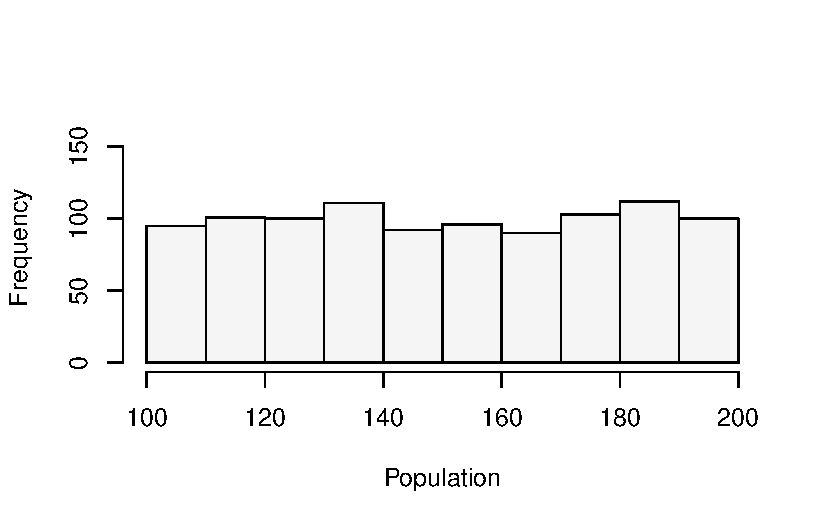
\includegraphics{./12-InferenceI_files/figure-pdf/unnamed-chunk-3-1.pdf}

}

\end{figure}

\begin{enumerate}
\def\labelenumi{\arabic{enumi}.}
\setcounter{enumi}{1}
\tightlist
\item
  Now let's create a for loop that allows us to sample the population
  several times. In fact, we will sample the population 1000 times and
  record the mean of the samples.
\end{enumerate}

\begin{Shaded}
\begin{Highlighting}[numbers=left,,]
\NormalTok{nrep}\OtherTok{\textless{}{-}}\DecValTok{1000}
\NormalTok{SampleMeans}\OtherTok{\textless{}{-}}\FunctionTok{c}\NormalTok{()}
\ControlFlowTok{for}\NormalTok{ (i }\ControlFlowTok{in} \DecValTok{1}\SpecialCharTok{:}\NormalTok{nrep)\{}
\NormalTok{  x}\OtherTok{\textless{}{-}}\FunctionTok{sample}\NormalTok{(Population,}\DecValTok{10}\NormalTok{,}\AttributeTok{replace=}\NormalTok{T)}
\NormalTok{  SampleMeans}\OtherTok{\textless{}{-}}\FunctionTok{c}\NormalTok{(SampleMeans,}\FunctionTok{mean}\NormalTok{(x))}
\NormalTok{\}}
\end{Highlighting}
\end{Shaded}

Now we can calculate the mean of the sample means in R:

\begin{Shaded}
\begin{Highlighting}[numbers=left,,]
\FunctionTok{mean}\NormalTok{(SampleMeans)}
\end{Highlighting}
\end{Shaded}

\begin{verbatim}
[1] 150.4177
\end{verbatim}

Note that the mean is very close to \emph{PopMean}. In the limit (that
is if we take many more samples), these two values are equal to each
other. Now let's calculate the standard deviation of the sample means.

\begin{Shaded}
\begin{Highlighting}[numbers=left,,]
\FunctionTok{sd}\NormalTok{(SampleMeans)}
\end{Highlighting}
\end{Shaded}

\begin{verbatim}
[1] 9.134147
\end{verbatim}

As you can see, the standard deviation is much lower. In fact, if we
take \emph{PopSD} and divide by 10 (the size of the sample), we should
get close to the standard deviation of the sample means.

\begin{Shaded}
\begin{Highlighting}[numbers=left,,]
\NormalTok{PopSD}\SpecialCharTok{/}\FunctionTok{sqrt}\NormalTok{(}\DecValTok{10}\NormalTok{)}
\end{Highlighting}
\end{Shaded}

\begin{verbatim}
[1] 9.233644
\end{verbatim}

\begin{enumerate}
\def\labelenumi{\arabic{enumi}.}
\setcounter{enumi}{2}
\tightlist
\item
  To create the histogram we use the \texttt{hist()} function once more:
\end{enumerate}

\begin{Shaded}
\begin{Highlighting}[numbers=left,,]
\FunctionTok{hist}\NormalTok{(SampleMeans, }\AttributeTok{main=}\StringTok{""}\NormalTok{, }\AttributeTok{ylim=}\FunctionTok{c}\NormalTok{(}\DecValTok{0}\NormalTok{,}\DecValTok{300}\NormalTok{), }\AttributeTok{col=}\StringTok{"\#F5F5F5"}\NormalTok{)}
\end{Highlighting}
\end{Shaded}

\begin{figure}[H]

{\centering 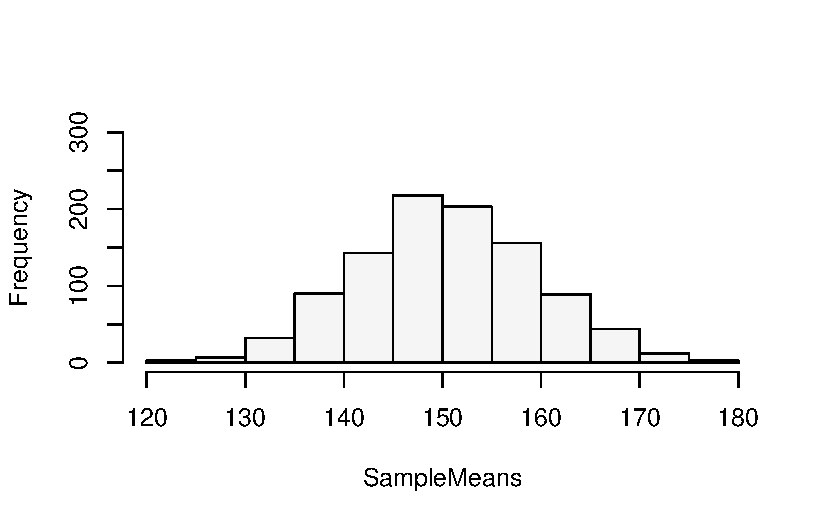
\includegraphics{./12-InferenceI_files/figure-pdf/unnamed-chunk-8-1.pdf}

}

\end{figure}

The distribution looks normal. To be clear, if the population follows a
uniform distribution, we have shown that the distribution of the sample
means is normal with a mean equal to the population mean and a smaller
standard deviation.\\
We can use the distribution of the sample means to calculate the
probability. Noting the the distribution is normal:

\begin{Shaded}
\begin{Highlighting}[numbers=left,,]
\FunctionTok{pnorm}\NormalTok{(}\DecValTok{160}\NormalTok{,}\FunctionTok{mean}\NormalTok{(SampleMeans),}\FunctionTok{sd}\NormalTok{(SampleMeans))}\SpecialCharTok{{-}}\FunctionTok{pnorm}\NormalTok{(}\DecValTok{140}\NormalTok{,}\FunctionTok{mean}\NormalTok{(SampleMeans),}\FunctionTok{sd}\NormalTok{(SampleMeans))}
\end{Highlighting}
\end{Shaded}

\begin{verbatim}
[1] 0.7258913
\end{verbatim}

There is a \(72.59\)\% probability that the sample mean is between
\(140\) and \(160\).

\hypertarget{exercise-2-21}{%
\subsection*{Exercise 2}\label{exercise-2-21}}
\addcontentsline{toc}{subsection}{Exercise 2}

\begin{blackbox}

\begin{enumerate}
\def\labelenumi{\arabic{enumi}.}
\tightlist
\item
  The expected value is \(80\) since it is equal to the mean of the
  population. The standard error is \(1.4\). The probability is
  \(98.38\)\%.
\end{enumerate}

\end{blackbox}

We can use R as a calculator to find the standard error.

\begin{Shaded}
\begin{Highlighting}[numbers=left,,]
\DecValTok{14}\SpecialCharTok{/}\FunctionTok{sqrt}\NormalTok{(}\DecValTok{100}\NormalTok{)}
\end{Highlighting}
\end{Shaded}

\begin{verbatim}
[1] 1.4
\end{verbatim}

We can use \texttt{pnorm()} to find the probability:

\begin{Shaded}
\begin{Highlighting}[numbers=left,,]
\FunctionTok{pnorm}\NormalTok{(}\DecValTok{85}\NormalTok{,}\DecValTok{80}\NormalTok{,}\FloatTok{1.4}\NormalTok{)}\SpecialCharTok{{-}}\FunctionTok{pnorm}\NormalTok{(}\DecValTok{77}\NormalTok{,}\DecValTok{80}\NormalTok{,}\FloatTok{1.4}\NormalTok{)}
\end{Highlighting}
\end{Shaded}

\begin{verbatim}
[1] 0.9837602
\end{verbatim}

\begin{blackbox}

\begin{enumerate}
\def\labelenumi{\arabic{enumi}.}
\setcounter{enumi}{1}
\tightlist
\item
  The probabilities are \(24.66\)\% and \(1.8\)\%.
\end{enumerate}

\end{blackbox}

For the first probability we can use a sample size of \(4\) and use the
standard error in the \texttt{pnorm()} function.

\begin{Shaded}
\begin{Highlighting}[numbers=left,,]
\FunctionTok{pnorm}\NormalTok{(}\DecValTok{35}\NormalTok{,}\FloatTok{33.8}\NormalTok{,}\FloatTok{3.5}\SpecialCharTok{/}\FunctionTok{sqrt}\NormalTok{(}\DecValTok{4}\NormalTok{),}\AttributeTok{lower.tail =}\NormalTok{ F)}
\end{Highlighting}
\end{Shaded}

\begin{verbatim}
[1] 0.2464466
\end{verbatim}

For the second probability we can first calculate the probability that a
randomly selected car has mpg greater than \(35\). In R:

\begin{Shaded}
\begin{Highlighting}[numbers=left,,]
\NormalTok{(p35}\OtherTok{\textless{}{-}}\FunctionTok{pnorm}\NormalTok{(}\DecValTok{35}\NormalTok{,}\FloatTok{33.8}\NormalTok{,}\FloatTok{3.5}\NormalTok{,}\AttributeTok{lower.tail =}\NormalTok{ F))}
\end{Highlighting}
\end{Shaded}

\begin{verbatim}
[1] 0.365853
\end{verbatim}

Since draws are independent we get:

\begin{Shaded}
\begin{Highlighting}[numbers=left,,]
\NormalTok{p35}\SpecialCharTok{\^{}}\DecValTok{4}
\end{Highlighting}
\end{Shaded}

\begin{verbatim}
[1] 0.01791539
\end{verbatim}

\hypertarget{exercise-3-21}{%
\subsection*{Exercise 3}\label{exercise-3-21}}
\addcontentsline{toc}{subsection}{Exercise 3}

\begin{blackbox}

\begin{enumerate}
\def\labelenumi{\arabic{enumi}.}
\tightlist
\item
  The expected value is \(0.75\), the same as the population. The
  standard error is \(\sqrt{p(1-p)/n}=0.03\). The probability for a
  sample of \(200\) is \(0.8975\).
\end{enumerate}

\end{blackbox}

The standard error is given by:

\begin{Shaded}
\begin{Highlighting}[numbers=left,,]
\FunctionTok{sqrt}\NormalTok{(}\FloatTok{0.75}\SpecialCharTok{*}\FloatTok{0.25}\SpecialCharTok{/}\DecValTok{200}\NormalTok{)}
\end{Highlighting}
\end{Shaded}

\begin{verbatim}
[1] 0.03061862
\end{verbatim}

In R we can use the \texttt{pnorm()} function one more time to find the
probability.

\begin{Shaded}
\begin{Highlighting}[numbers=left,,]
\FunctionTok{pnorm}\NormalTok{(}\FloatTok{0.8}\NormalTok{,}\FloatTok{0.75}\NormalTok{,}\FunctionTok{sqrt}\NormalTok{(}\FloatTok{0.75}\SpecialCharTok{*}\FloatTok{0.25}\SpecialCharTok{/}\DecValTok{200}\NormalTok{))}\SpecialCharTok{{-}}\FunctionTok{pnorm}\NormalTok{(}\FloatTok{0.7}\NormalTok{,}\FloatTok{0.75}\NormalTok{,}\FunctionTok{sqrt}\NormalTok{(}\FloatTok{0.75}\SpecialCharTok{*}\FloatTok{0.25}\SpecialCharTok{/}\DecValTok{200}\NormalTok{))}
\end{Highlighting}
\end{Shaded}

\begin{verbatim}
[1] 0.8975296
\end{verbatim}

\begin{blackbox}

\begin{enumerate}
\def\labelenumi{\arabic{enumi}.}
\setcounter{enumi}{1}
\tightlist
\item
  The probability with a sample of \(50\) is \(69.29\)\%. When the
  sample is \(200\) the probability is \(84.33\)\%. As the sample size
  increases the standard error goes down. This means that the
  distribution of the sample proportions gets tighter and there is more
  area to the right of \(\bar{p}=0.2\).
\end{enumerate}

\end{blackbox}

In R we can use the \texttt{pnorm()} function one more time with a mean
of \(0.2\) and \(n=50\).

\begin{Shaded}
\begin{Highlighting}[numbers=left,,]
\FunctionTok{pnorm}\NormalTok{(}\FloatTok{0.2}\NormalTok{,}\FloatTok{0.23}\NormalTok{,}\FunctionTok{sqrt}\NormalTok{(}\FloatTok{0.23}\SpecialCharTok{*}\FloatTok{0.77}\SpecialCharTok{/}\DecValTok{50}\NormalTok{),}\AttributeTok{lower.tail =}\NormalTok{ F)}
\end{Highlighting}
\end{Shaded}

\begin{verbatim}
[1] 0.6928964
\end{verbatim}

Updating the code so that \(n=200\) yields:

\begin{Shaded}
\begin{Highlighting}[numbers=left,,]
\FunctionTok{pnorm}\NormalTok{(}\FloatTok{0.2}\NormalTok{,}\FloatTok{0.23}\NormalTok{,}\FunctionTok{sqrt}\NormalTok{(}\FloatTok{0.23}\SpecialCharTok{*}\FloatTok{0.77}\SpecialCharTok{/}\DecValTok{200}\NormalTok{),}\AttributeTok{lower.tail =}\NormalTok{ F)}
\end{Highlighting}
\end{Shaded}

\begin{verbatim}
[1] 0.8433098
\end{verbatim}

\hypertarget{exercise-4-9}{%
\subsection*{Exercise 4}\label{exercise-4-9}}
\addcontentsline{toc}{subsection}{Exercise 4}

\begin{blackbox}

\begin{enumerate}
\def\labelenumi{\arabic{enumi}.}
\tightlist
\item
  The process seems to be out of control. In the early samples, the
  machine is not filling the cans with enough drink. Although, in the
  later periods the machine reverts back to the expected performance, it
  seems unlikely that it will remain functioning correctly.
\end{enumerate}

\end{blackbox}

Let's start by calculating the upper and lower limits in R.

\begin{Shaded}
\begin{Highlighting}[numbers=left,,]
\NormalTok{dataEx1}\OtherTok{\textless{}{-}}\FunctionTok{c}\NormalTok{(}\DecValTok{310}\NormalTok{,}\DecValTok{315}\NormalTok{,}\DecValTok{325}\NormalTok{,}\DecValTok{330}\NormalTok{,}\DecValTok{328}\NormalTok{,}\DecValTok{347}\NormalTok{,}\DecValTok{339}\NormalTok{,}\DecValTok{350}\NormalTok{)}
\NormalTok{ulEx1}\OtherTok{\textless{}{-}}\DecValTok{350}\SpecialCharTok{+}\DecValTok{3}\SpecialCharTok{*}\NormalTok{(}\DecValTok{10}\SpecialCharTok{/}\FunctionTok{sqrt}\NormalTok{(}\DecValTok{10}\NormalTok{))}
\NormalTok{llEx1}\OtherTok{\textless{}{-}}\DecValTok{350{-}3}\SpecialCharTok{*}\NormalTok{(}\DecValTok{10}\SpecialCharTok{/}\FunctionTok{sqrt}\NormalTok{(}\DecValTok{10}\NormalTok{))}
\end{Highlighting}
\end{Shaded}

We can graph the samples and the limits to determine the stability of
the production process.

\begin{Shaded}
\begin{Highlighting}[numbers=left,,]
\FunctionTok{plot}\NormalTok{(dataEx1, }\AttributeTok{type=}\StringTok{"b"}\NormalTok{, }\AttributeTok{ylab=}\StringTok{"Mean Gallons"}\NormalTok{,}
     \AttributeTok{xlab=}\StringTok{"Period"}\NormalTok{, }\AttributeTok{pch=}\DecValTok{21}\NormalTok{, }\AttributeTok{bg=}\StringTok{"blue"}\NormalTok{,}\AttributeTok{ylim=}\FunctionTok{c}\NormalTok{(}\DecValTok{280}\NormalTok{,}\DecValTok{380}\NormalTok{))}
\FunctionTok{abline}\NormalTok{(}\AttributeTok{h=}\NormalTok{ulEx1,}\AttributeTok{col=}\StringTok{"red"}\NormalTok{)}
\FunctionTok{abline}\NormalTok{(}\AttributeTok{h=}\NormalTok{llEx1,}\AttributeTok{col=}\StringTok{"red"}\NormalTok{)}
\end{Highlighting}
\end{Shaded}

\begin{figure}[H]

{\centering 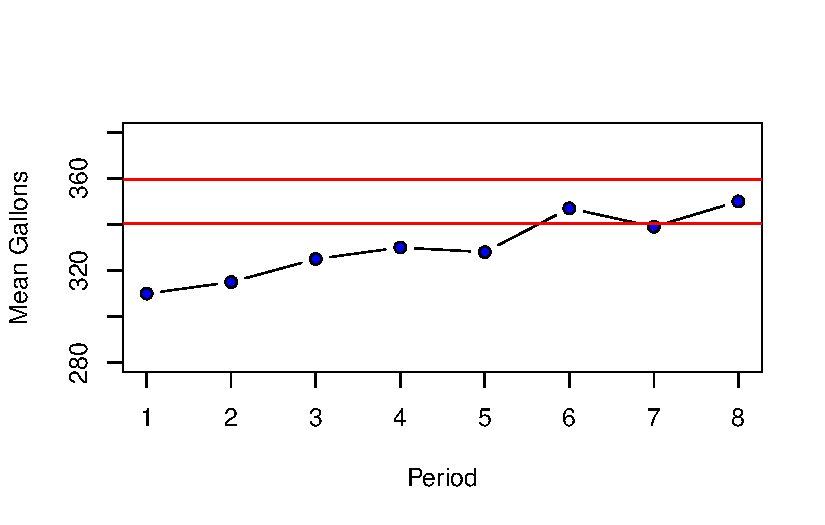
\includegraphics{./12-InferenceI_files/figure-pdf/unnamed-chunk-20-1.pdf}

}

\end{figure}

\begin{blackbox}

\begin{enumerate}
\def\labelenumi{\arabic{enumi}.}
\setcounter{enumi}{1}
\tightlist
\item
  Good Dolls production looks good. All proportions fall between three
  standard errors of the mean.
\end{enumerate}

\end{blackbox}

Once more we can calculate upper and lower limits for the proportions.

\begin{Shaded}
\begin{Highlighting}[numbers=left,,]
\NormalTok{dataEx2}\OtherTok{\textless{}{-}}\FunctionTok{c}\NormalTok{(}\FloatTok{0.009}\NormalTok{,}\FloatTok{0.012}\NormalTok{,}\FloatTok{0.008}\NormalTok{,}\FloatTok{0.011}\NormalTok{,}\FloatTok{0.0102}\NormalTok{)}
\NormalTok{ulEx2}\OtherTok{\textless{}{-}}\FloatTok{0.01}\SpecialCharTok{+}\DecValTok{3}\SpecialCharTok{*}\FunctionTok{sqrt}\NormalTok{(}\FloatTok{0.01}\SpecialCharTok{*}\FloatTok{0.99}\SpecialCharTok{/}\DecValTok{1000}\NormalTok{)}
\NormalTok{llEx2}\OtherTok{\textless{}{-}}\FloatTok{0.01}\DecValTok{{-}3}\SpecialCharTok{*}\FunctionTok{sqrt}\NormalTok{(}\FloatTok{0.01}\SpecialCharTok{*}\FloatTok{0.99}\SpecialCharTok{/}\DecValTok{1000}\NormalTok{)}
\end{Highlighting}
\end{Shaded}

Graphing the results in R we can observe the production process and the
sample proportions.

\begin{Shaded}
\begin{Highlighting}[numbers=left,,]
\FunctionTok{plot}\NormalTok{(dataEx2, }\AttributeTok{type=}\StringTok{"b"}\NormalTok{, }\AttributeTok{ylab=}\StringTok{"Proportion Defective"}\NormalTok{,}
     \AttributeTok{xlab=}\StringTok{"Period"}\NormalTok{, }\AttributeTok{pch=}\DecValTok{21}\NormalTok{, }\AttributeTok{bg=}\StringTok{"blue"}\NormalTok{,}\AttributeTok{ylim=}\FunctionTok{c}\NormalTok{(}\DecValTok{0}\NormalTok{,}\FloatTok{0.02}\NormalTok{))}
\FunctionTok{abline}\NormalTok{(}\AttributeTok{h=}\NormalTok{ulEx2,}\AttributeTok{col=}\StringTok{"red"}\NormalTok{)}
\FunctionTok{abline}\NormalTok{(}\AttributeTok{h=}\NormalTok{llEx2,}\AttributeTok{col=}\StringTok{"red"}\NormalTok{)}
\end{Highlighting}
\end{Shaded}

\begin{figure}[H]

{\centering 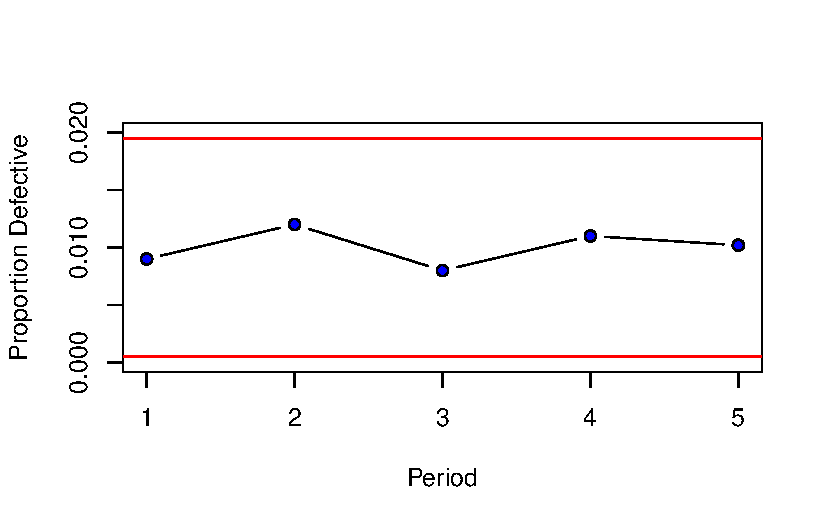
\includegraphics{./12-InferenceI_files/figure-pdf/unnamed-chunk-22-1.pdf}

}

\end{figure}

\hypertarget{inference-ii}{%
\chapter{Inference II}\label{inference-ii}}

\hypertarget{concepts-11}{%
\section{Concepts}\label{concepts-11}}

\hypertarget{confidence-intervals}{%
\subsection*{Confidence Intervals}\label{confidence-intervals}}
\addcontentsline{toc}{subsection}{Confidence Intervals}

A \textbf{confidence interval} provides a range of values that, with a
certain level of confidence, contains the population parameter of
interest. For proper confidence intervals ensure that the sampling
distributions are normal.

A \(95\)\% \textbf{confidence level}, indicates that if the interval
were constructed many times (from independent samples of the
population), it would include the true population parameter \(95\)\% of
the time.

A \textbf{significance level} (\(\alpha\)) of \(5\)\%, means that the
confidence interval would would not include the true population
parameter \(5\)\% of the time.

The interval for the population mean when the population standard
deviation is unknown is given by
\(\bar x \pm t_{\alpha/2} \frac {s}{n}\), where \(\bar x\) is the point
estimate, \(t_{a/2} \frac {s}{n}\) is the margin of error, and
\(\alpha\) is the allowed probability that the interval does not include
\(\mu\).

The interval for the population proportion mean is given by
\(\bar p \pm z_{\alpha/2} \sqrt{\frac {\bar p (1-\bar p)}{n}}\).

\hypertarget{useful-r-functions-11}{%
\subsection*{Useful R Functions}\label{useful-r-functions-11}}
\addcontentsline{toc}{subsection}{Useful R Functions}

The \texttt{qnorm()} and \texttt{qt()} functions calculate quartiles for
the normal and \(t\) distributions, respectively.

The \texttt{if()} function creates a conditional statement in R.

\hypertarget{exercises-11}{%
\section{Exercises}\label{exercises-11}}

The following exercises will help you test your knowledge on Statistical
Inference. In particular, the exercises work on:

\begin{itemize}
\item
  Simulating confidence intervals.
\item
  Estimating confidence intervals in R.
\item
  Estimating confidence intervals for proportions.
\end{itemize}

Answers are provided below. Try not to peak until you have a formulated
your own answer and double checked your work for any mistakes.

\hypertarget{exercise-1-22}{%
\subsection*{Exercise 1}\label{exercise-1-22}}
\addcontentsline{toc}{subsection}{Exercise 1}

In this exercise you will be simulating confidence intervals.

\begin{enumerate}
\def\labelenumi{\arabic{enumi}.}
\item
  Set the seed to \(9\). Create a random sample of 1000 data points and
  store it in an object called \emph{Population}. Use the exponential
  distribution with rate of \(0.02\) to generate the data. Calculate the
  mean and standard deviation of \emph{Population} and call them
  \emph{PopMean} and \emph{PopSD} respectively. What are the mean and
  standard deviation of \emph{Population}?
\item
  Create a for loop (with 10,000 iterations) that takes a sample of 50
  points from \emph{Population}, calculates the mean, and then stores
  the result in a vector called \emph{SampleMeans}. What is the mean of
  the \emph{SampleMeans}?
\item
  Create a \(90\)\% confidence interval using the first data point in
  the \emph{SampleMeans} vector. Does the confidence interval include
  \emph{PopMean}?
\item
  Now take the minimum of the \emph{SampleMeans} vector. Create a new
  \(90\)\% confidence interval. Does the interval include
  \emph{PopMean}? Out of the \(10,000\) intervals that you could
  construct with the vector \emph{SampleMeans}, how many would you
  expect to include \emph{PopMean}?
\end{enumerate}

\hypertarget{exercise-2-22}{%
\subsection*{Exercise 2}\label{exercise-2-22}}
\addcontentsline{toc}{subsection}{Exercise 2}

\begin{enumerate}
\def\labelenumi{\arabic{enumi}.}
\item
  A random sample of \(24\) observations is used to estimate the
  population mean. The sample mean is \(104.6\) and the standard
  deviation is \(28.8\). The population is normally distributed.
  Construct a \(90\)\% and \(95\)\% confidence interval for the
  population mean. How does the confidence level affect the size of the
  interval?
\item
  A random sample from a normally distributed population yields a mean
  of \(48.68\) and a standard deviation of \(33.64\). Compute a \(95\)\%
  confidence interval assuming a) that the sample size is \(16\) and b)
  the sample size is \(25\). What happens to the confidence interval as
  the sample size increases?
\end{enumerate}

\hypertarget{exercise-3-22}{%
\subsection*{Exercise 3}\label{exercise-3-22}}
\addcontentsline{toc}{subsection}{Exercise 3}

You will need the \textbf{sleep} data set for this problem. The data is
built into R, and displays the effect of two sleep inducing drugs on
students. Calculate a \(95\)\% confidence interval for group 1 and for
group 2. Which drug would you expect to be more effective at increasing
sleeping times?

\hypertarget{exercise-4-10}{%
\subsection*{Exercise 4}\label{exercise-4-10}}
\addcontentsline{toc}{subsection}{Exercise 4}

\begin{enumerate}
\def\labelenumi{\arabic{enumi}.}
\item
  A random sample of \(100\) observations results in \(40\) successes.
  Construct a \(90\)\% and \(95\)\% confidence interval for the
  population proportion. Can we conclude at either confidence level that
  the population proportion differs from \(0.5\)?
\item
  You will need the \textbf{HairEyeColor} data set for this problem. The
  data is built into R, and displays the distribution of hair and eye
  color for \(592\) statistics students. Construct a \(95\) confidence
  interval for the proportion of Hazel eye color students.
\end{enumerate}

\hypertarget{answers-11}{%
\section{Answers}\label{answers-11}}

\hypertarget{exercise-1-23}{%
\subsection*{Exercise 1}\label{exercise-1-23}}
\addcontentsline{toc}{subsection}{Exercise 1}

\begin{blackbox}

\begin{enumerate}
\def\labelenumi{\arabic{enumi}.}
\tightlist
\item
  The mean of \emph{Population} is \(48.61\). The standard deviation is
  \(47.94\).
\end{enumerate}

\end{blackbox}

Start by generating values from the exponential distribution. You can
use the \texttt{rexp()} function in R to do this. Setting the seed to
\(9\) yields:

\begin{Shaded}
\begin{Highlighting}[numbers=left,,]
\FunctionTok{set.seed}\NormalTok{(}\DecValTok{9}\NormalTok{)}
\NormalTok{Population}\OtherTok{\textless{}{-}}\FunctionTok{rexp}\NormalTok{(}\DecValTok{1000}\NormalTok{,}\FloatTok{0.02}\NormalTok{)}
\end{Highlighting}
\end{Shaded}

The population mean is:

\begin{Shaded}
\begin{Highlighting}[numbers=left,,]
\NormalTok{(PopMean}\OtherTok{\textless{}{-}}\FunctionTok{mean}\NormalTok{(Population))}
\end{Highlighting}
\end{Shaded}

\begin{verbatim}
[1] 48.61053
\end{verbatim}

The standard deviation is:

\begin{Shaded}
\begin{Highlighting}[numbers=left,,]
\NormalTok{(PopSD}\OtherTok{\textless{}{-}}\FunctionTok{sd}\NormalTok{(Population))}
\end{Highlighting}
\end{Shaded}

\begin{verbatim}
[1] 47.94411
\end{verbatim}

\begin{blackbox}

\begin{enumerate}
\def\labelenumi{\arabic{enumi}.}
\setcounter{enumi}{1}
\tightlist
\item
  The mean is very close to the population mean \(48.83\). The standard
  deviation is \(6.83\).
\end{enumerate}

\end{blackbox}

In R you can use a for loop to create the vector of sample means.

\begin{Shaded}
\begin{Highlighting}[numbers=left,,]
\NormalTok{nrep}\OtherTok{\textless{}{-}}\DecValTok{10000}
\NormalTok{SampleMeans}\OtherTok{\textless{}{-}}\FunctionTok{c}\NormalTok{()}
\ControlFlowTok{for}\NormalTok{ (i }\ControlFlowTok{in} \DecValTok{1}\SpecialCharTok{:}\NormalTok{nrep)\{}
\NormalTok{  x}\OtherTok{\textless{}{-}}\FunctionTok{sample}\NormalTok{(Population,}\DecValTok{50}\NormalTok{,}\AttributeTok{replace=}\NormalTok{T)}
\NormalTok{  SampleMeans}\OtherTok{\textless{}{-}}\FunctionTok{c}\NormalTok{(SampleMeans,}\FunctionTok{mean}\NormalTok{(x))}
\NormalTok{\}}
\end{Highlighting}
\end{Shaded}

The mean of \emph{SampleMeans} is:

\begin{Shaded}
\begin{Highlighting}[numbers=left,,]
\NormalTok{(xbar}\OtherTok{\textless{}{-}}\FunctionTok{mean}\NormalTok{(SampleMeans))}
\end{Highlighting}
\end{Shaded}

\begin{verbatim}
[1] 48.7005
\end{verbatim}

The standard deviation is:

\begin{Shaded}
\begin{Highlighting}[numbers=left,,]
\NormalTok{(Standard}\OtherTok{\textless{}{-}}\FunctionTok{sd}\NormalTok{(SampleMeans))}
\end{Highlighting}
\end{Shaded}

\begin{verbatim}
[1] 6.827595
\end{verbatim}

\begin{blackbox}

\begin{enumerate}
\def\labelenumi{\arabic{enumi}.}
\setcounter{enumi}{2}
\tightlist
\item
  The confidence interval is {[}\(47.71\),\(70.17\){]}. Since the
  population mean is equal to \(48.61\), the confidence interval does
  include the population mean.
\end{enumerate}

\end{blackbox}

Let's construct the upper an lower limits of the interval in R.

\begin{Shaded}
\begin{Highlighting}[numbers=left,,]
\NormalTok{(ll}\OtherTok{\textless{}{-}}\NormalTok{SampleMeans[}\DecValTok{1}\NormalTok{]}\SpecialCharTok{+}\FunctionTok{qnorm}\NormalTok{(}\FloatTok{0.05}\NormalTok{)}\SpecialCharTok{*}\NormalTok{Standard)}
\end{Highlighting}
\end{Shaded}

\begin{verbatim}
[1] 47.71385
\end{verbatim}

\begin{Shaded}
\begin{Highlighting}[numbers=left,,]
\NormalTok{(ul}\OtherTok{\textless{}{-}}\NormalTok{SampleMeans[}\DecValTok{1}\NormalTok{]}\SpecialCharTok{{-}}\FunctionTok{qnorm}\NormalTok{(}\FloatTok{0.05}\NormalTok{)}\SpecialCharTok{*}\NormalTok{Standard)}
\end{Highlighting}
\end{Shaded}

\begin{verbatim}
[1] 70.17464
\end{verbatim}

\begin{blackbox}

\begin{enumerate}
\def\labelenumi{\arabic{enumi}.}
\setcounter{enumi}{3}
\tightlist
\item
  The confidence interval is {[}\(14.86\),\(37.32\){]}. This interval
  does not include the population mean of \(48.61\). Out of the
  \(10,000\) confidence intervals, one would expect about \(9,000\) to
  include the population mean.
\end{enumerate}

\end{blackbox}

Let's find the confidence interval limits using R.

\begin{Shaded}
\begin{Highlighting}[numbers=left,,]
\NormalTok{(Minll}\OtherTok{\textless{}{-}}\FunctionTok{min}\NormalTok{(SampleMeans)}\SpecialCharTok{+}\FunctionTok{qnorm}\NormalTok{(}\FloatTok{0.05}\NormalTok{)}\SpecialCharTok{*}\NormalTok{Standard)}
\end{Highlighting}
\end{Shaded}

\begin{verbatim}
[1] 14.85631
\end{verbatim}

\begin{Shaded}
\begin{Highlighting}[numbers=left,,]
\NormalTok{(Minul}\OtherTok{\textless{}{-}}\FunctionTok{min}\NormalTok{(SampleMeans)}\SpecialCharTok{{-}}\FunctionTok{qnorm}\NormalTok{(}\FloatTok{0.05}\NormalTok{)}\SpecialCharTok{*}\NormalTok{Standard)}
\end{Highlighting}
\end{Shaded}

\begin{verbatim}
[1] 37.31709
\end{verbatim}

We can confirm in R that about \(9,000\) of the intervals include
\emph{PopMean}. Once more, let's use a for loop to construct confidence
intervals for each element in \emph{SampleMeans} and check whether the
\emph{PopMean} is included. The count variable keeps track of how many
intervals include the population mean.

\begin{Shaded}
\begin{Highlighting}[numbers=left,,]
\NormalTok{count}\OtherTok{=}\DecValTok{0}

\ControlFlowTok{for}\NormalTok{ (i }\ControlFlowTok{in}\NormalTok{ SampleMeans)\{}
\NormalTok{  (ll}\OtherTok{\textless{}{-}}\NormalTok{i}\SpecialCharTok{+}\FunctionTok{qnorm}\NormalTok{(}\FloatTok{0.05}\NormalTok{)}\SpecialCharTok{*}\NormalTok{Standard)}
\NormalTok{  (ul}\OtherTok{\textless{}{-}}\NormalTok{i}\SpecialCharTok{{-}}\FunctionTok{qnorm}\NormalTok{(}\FloatTok{0.05}\NormalTok{)}\SpecialCharTok{*}\NormalTok{Standard)}
  \ControlFlowTok{if}\NormalTok{ (PopMean}\SpecialCharTok{\textless{}=}\NormalTok{ul }\SpecialCharTok{\&}\NormalTok{ PopMean}\SpecialCharTok{\textgreater{}=}\NormalTok{ll)\{}
\NormalTok{    count}\OtherTok{=}\NormalTok{count}\SpecialCharTok{+}\DecValTok{1}
\NormalTok{  \}}
\NormalTok{\}}

\NormalTok{count}
\end{Highlighting}
\end{Shaded}

\begin{verbatim}
[1] 8978
\end{verbatim}

\hypertarget{exercise-2-23}{%
\subsection*{Exercise 2}\label{exercise-2-23}}
\addcontentsline{toc}{subsection}{Exercise 2}

\begin{blackbox}

\begin{enumerate}
\def\labelenumi{\arabic{enumi}.}
\tightlist
\item
  The \(90\)\% confidence interval is {[}\(94.52\),\(114.67\){]} and the
  \(95\)\% confidence interval is {[}\(114.68\),\(116.76\){]}. The
  larger the confidence level, the larger the interval.
\end{enumerate}

\end{blackbox}

Let's construct the intervals using R. Since the population standard
deviation is unknown we will use the t-distribution. The interval is
constructed as \(\bar{x}\pm t_{\alpha/2} \frac{s}{\sqrt{n}}\).

\begin{Shaded}
\begin{Highlighting}[numbers=left,,]
\NormalTok{(ul90}\OtherTok{\textless{}{-}}\FloatTok{104.6}\SpecialCharTok{{-}}\FunctionTok{qt}\NormalTok{(}\FloatTok{0.05}\NormalTok{,}\DecValTok{23}\NormalTok{)}\SpecialCharTok{*}\FloatTok{28.8}\SpecialCharTok{/}\FunctionTok{sqrt}\NormalTok{(}\DecValTok{24}\NormalTok{))}
\end{Highlighting}
\end{Shaded}

\begin{verbatim}
[1] 114.6755
\end{verbatim}

\begin{Shaded}
\begin{Highlighting}[numbers=left,,]
\NormalTok{(ll90}\OtherTok{\textless{}{-}}\FloatTok{104.6}\SpecialCharTok{+}\FunctionTok{qt}\NormalTok{(}\FloatTok{0.05}\NormalTok{,}\DecValTok{23}\NormalTok{)}\SpecialCharTok{*}\FloatTok{28.8}\SpecialCharTok{/}\FunctionTok{sqrt}\NormalTok{(}\DecValTok{24}\NormalTok{))}
\end{Highlighting}
\end{Shaded}

\begin{verbatim}
[1] 94.52453
\end{verbatim}

For the \(95\)\% confidence interval we adjust the significance level
accordingly.

\begin{Shaded}
\begin{Highlighting}[numbers=left,,]
\NormalTok{(ul95}\OtherTok{\textless{}{-}}\FloatTok{104.6}\SpecialCharTok{{-}}\FunctionTok{qt}\NormalTok{(}\FloatTok{0.025}\NormalTok{,}\DecValTok{23}\NormalTok{)}\SpecialCharTok{*}\FloatTok{28.8}\SpecialCharTok{/}\FunctionTok{sqrt}\NormalTok{(}\DecValTok{24}\NormalTok{))}
\end{Highlighting}
\end{Shaded}

\begin{verbatim}
[1] 116.7612
\end{verbatim}

\begin{Shaded}
\begin{Highlighting}[numbers=left,,]
\NormalTok{(ll95}\OtherTok{\textless{}{-}}\FloatTok{104.6}\SpecialCharTok{+}\FunctionTok{qt}\NormalTok{(}\FloatTok{0.025}\NormalTok{,}\DecValTok{23}\NormalTok{)}\SpecialCharTok{*}\FloatTok{28.8}\SpecialCharTok{/}\FunctionTok{sqrt}\NormalTok{(}\DecValTok{24}\NormalTok{))}
\end{Highlighting}
\end{Shaded}

\begin{verbatim}
[1] 92.43883
\end{verbatim}

\begin{blackbox}

\begin{enumerate}
\def\labelenumi{\arabic{enumi}.}
\setcounter{enumi}{1}
\tightlist
\item
  The confidence interval for a sample size of \(16\) is
  {[}\(30.75\),\(66.61\){]}. The confidence interval when the sample
  size is \(25\) is {[}\(34.79\),\(62.57\){]}. As the sample size gets
  larger, the confidence interval gets narrower and more precise.
\end{enumerate}

\end{blackbox}

Let's use R again to calculate the confidence interval. For a sample
size of \(16\) the interval is:

\begin{Shaded}
\begin{Highlighting}[numbers=left,,]
\NormalTok{(ul16}\OtherTok{\textless{}{-}}\FloatTok{48.68}\SpecialCharTok{{-}}\FunctionTok{qt}\NormalTok{(}\FloatTok{0.025}\NormalTok{,}\DecValTok{15}\NormalTok{)}\SpecialCharTok{*}\FloatTok{33.64}\SpecialCharTok{/}\FunctionTok{sqrt}\NormalTok{(}\DecValTok{16}\NormalTok{))}
\end{Highlighting}
\end{Shaded}

\begin{verbatim}
[1] 66.60549
\end{verbatim}

\begin{Shaded}
\begin{Highlighting}[numbers=left,,]
\NormalTok{(ll16}\OtherTok{\textless{}{-}}\FloatTok{48.68}\SpecialCharTok{+}\FunctionTok{qt}\NormalTok{(}\FloatTok{0.025}\NormalTok{,}\DecValTok{15}\NormalTok{)}\SpecialCharTok{*}\FloatTok{33.64}\SpecialCharTok{/}\FunctionTok{sqrt}\NormalTok{(}\DecValTok{16}\NormalTok{))}
\end{Highlighting}
\end{Shaded}

\begin{verbatim}
[1] 30.75451
\end{verbatim}

Increasing the ample size to \(25\) yields:

\begin{Shaded}
\begin{Highlighting}[numbers=left,,]
\NormalTok{(ul25}\OtherTok{\textless{}{-}}\FloatTok{48.68}\SpecialCharTok{{-}}\FunctionTok{qt}\NormalTok{(}\FloatTok{0.025}\NormalTok{,}\DecValTok{24}\NormalTok{)}\SpecialCharTok{*}\FloatTok{33.64}\SpecialCharTok{/}\FunctionTok{sqrt}\NormalTok{(}\DecValTok{25}\NormalTok{))}
\end{Highlighting}
\end{Shaded}

\begin{verbatim}
[1] 62.56591
\end{verbatim}

\begin{Shaded}
\begin{Highlighting}[numbers=left,,]
\NormalTok{(ll25}\OtherTok{\textless{}{-}}\FloatTok{48.68}\SpecialCharTok{+}\FunctionTok{qt}\NormalTok{(}\FloatTok{0.025}\NormalTok{,}\DecValTok{24}\NormalTok{)}\SpecialCharTok{*}\FloatTok{33.64}\SpecialCharTok{/}\FunctionTok{sqrt}\NormalTok{(}\DecValTok{25}\NormalTok{))}
\end{Highlighting}
\end{Shaded}

\begin{verbatim}
[1] 34.79409
\end{verbatim}

\hypertarget{exercise-3-23}{%
\subsection*{Exercise 3}\label{exercise-3-23}}
\addcontentsline{toc}{subsection}{Exercise 3}

\begin{blackbox}

\begin{enumerate}
\def\labelenumi{\arabic{enumi}.}
\tightlist
\item
  The 95\% confidence interval for group 1 is {[}\(-0.36\),\(1.86\){]}.
\end{enumerate}

\end{blackbox}

Let's first calculate the standard error for group 1.

\begin{Shaded}
\begin{Highlighting}[numbers=left,,]
\NormalTok{(se1}\OtherTok{\textless{}{-}}\FunctionTok{sd}\NormalTok{(sleep}\SpecialCharTok{$}\NormalTok{extra[sleep}\SpecialCharTok{$}\NormalTok{group}\SpecialCharTok{==}\DecValTok{1}\NormalTok{])}\SpecialCharTok{/}\FunctionTok{sqrt}\NormalTok{(}\FunctionTok{length}\NormalTok{(sleep}\SpecialCharTok{$}\NormalTok{extra[sleep}\SpecialCharTok{$}\NormalTok{group}\SpecialCharTok{==}\DecValTok{1}\NormalTok{])))}
\end{Highlighting}
\end{Shaded}

\begin{verbatim}
[1] 0.5657345
\end{verbatim}

We can now use the standard error to estimate the lower and upper limits
of the confidence interval.

\begin{Shaded}
\begin{Highlighting}[numbers=left,,]
\NormalTok{(ll1}\OtherTok{\textless{}{-}}\FunctionTok{mean}\NormalTok{(sleep}\SpecialCharTok{$}\NormalTok{extra[sleep}\SpecialCharTok{$}\NormalTok{group}\SpecialCharTok{==}\DecValTok{1}\NormalTok{])}\SpecialCharTok{+}\FunctionTok{qnorm}\NormalTok{(}\FloatTok{0.025}\NormalTok{)}\SpecialCharTok{*}\NormalTok{se1)}
\end{Highlighting}
\end{Shaded}

\begin{verbatim}
[1] -0.3588193
\end{verbatim}

\begin{Shaded}
\begin{Highlighting}[numbers=left,,]
\NormalTok{(ul1}\OtherTok{\textless{}{-}}\FunctionTok{mean}\NormalTok{(sleep}\SpecialCharTok{$}\NormalTok{extra[sleep}\SpecialCharTok{$}\NormalTok{group}\SpecialCharTok{==}\DecValTok{1}\NormalTok{])}\SpecialCharTok{{-}}\FunctionTok{qnorm}\NormalTok{(}\FloatTok{0.025}\NormalTok{)}\SpecialCharTok{*}\NormalTok{se1)}
\end{Highlighting}
\end{Shaded}

\begin{verbatim}
[1] 1.858819
\end{verbatim}

\begin{blackbox}

\begin{enumerate}
\def\labelenumi{\arabic{enumi}.}
\setcounter{enumi}{1}
\tightlist
\item
  The 95\% confidence interval for group 2 is {[}\(1.09\),\(3.57\){]}.
\end{enumerate}

\end{blackbox}

Let's repeat the procedure for group 2. Start by finding the standard
error.

\begin{Shaded}
\begin{Highlighting}[numbers=left,,]
\NormalTok{(se2}\OtherTok{\textless{}{-}}\FunctionTok{sd}\NormalTok{(sleep}\SpecialCharTok{$}\NormalTok{extra[sleep}\SpecialCharTok{$}\NormalTok{group}\SpecialCharTok{==}\DecValTok{2}\NormalTok{])}\SpecialCharTok{/}\FunctionTok{sqrt}\NormalTok{(}\FunctionTok{length}\NormalTok{(sleep}\SpecialCharTok{$}\NormalTok{extra[sleep}\SpecialCharTok{$}\NormalTok{group}\SpecialCharTok{==}\DecValTok{2}\NormalTok{])))}
\end{Highlighting}
\end{Shaded}

\begin{verbatim}
[1] 0.6331666
\end{verbatim}

Using the standard error we can complete the confidence interval.

\begin{Shaded}
\begin{Highlighting}[numbers=left,,]
\NormalTok{(ll2}\OtherTok{\textless{}{-}}\FunctionTok{mean}\NormalTok{(sleep}\SpecialCharTok{$}\NormalTok{extra[sleep}\SpecialCharTok{$}\NormalTok{group}\SpecialCharTok{==}\DecValTok{2}\NormalTok{])}\SpecialCharTok{+}\FunctionTok{qnorm}\NormalTok{(}\FloatTok{0.025}\NormalTok{)}\SpecialCharTok{*}\NormalTok{se2)}
\end{Highlighting}
\end{Shaded}

\begin{verbatim}
[1] 1.089016
\end{verbatim}

\begin{Shaded}
\begin{Highlighting}[numbers=left,,]
\NormalTok{(ul2}\OtherTok{\textless{}{-}}\FunctionTok{mean}\NormalTok{(sleep}\SpecialCharTok{$}\NormalTok{extra[sleep}\SpecialCharTok{$}\NormalTok{group}\SpecialCharTok{==}\DecValTok{2}\NormalTok{])}\SpecialCharTok{{-}}\FunctionTok{qnorm}\NormalTok{(}\FloatTok{0.025}\NormalTok{)}\SpecialCharTok{*}\NormalTok{se2)}
\end{Highlighting}
\end{Shaded}

\begin{verbatim}
[1] 3.570984
\end{verbatim}

\begin{blackbox}

\begin{enumerate}
\def\labelenumi{\arabic{enumi}.}
\setcounter{enumi}{2}
\tightlist
\item
  Drug 2. Drug 2 does not include zero in the interval, and the interval
  is to the right of zero. It is unlikely, that drug 2 has no effect on
  students sleeping time. Additionally, Drug 2's mean increase in
  sleeping hours is \(2.33\) vs.~\(0.75\) for drug 1.
\end{enumerate}

\end{blackbox}

\hypertarget{exercise-4-11}{%
\subsection*{Exercise 4}\label{exercise-4-11}}
\addcontentsline{toc}{subsection}{Exercise 4}

\begin{blackbox}

\begin{enumerate}
\def\labelenumi{\arabic{enumi}.}
\tightlist
\item
  The 90\% and 95\% confidence intervals are {[}\(0.319\),\(0.481\){]},
  and {[}\(0.304\),\(0.496\){]} respectively. Since they do not include
  0.5, we can conclude that the population proportion is significantly
  different from 0.5.
\end{enumerate}

\end{blackbox}

We can create an object that stores the sample proportion and sample in
R:

\begin{Shaded}
\begin{Highlighting}[numbers=left,,]
\NormalTok{(p}\OtherTok{\textless{}{-}}\FloatTok{0.4}\NormalTok{)}
\end{Highlighting}
\end{Shaded}

\begin{verbatim}
[1] 0.4
\end{verbatim}

\begin{Shaded}
\begin{Highlighting}[numbers=left,,]
\NormalTok{(n}\OtherTok{\textless{}{-}}\DecValTok{100}\NormalTok{)}
\end{Highlighting}
\end{Shaded}

\begin{verbatim}
[1] 100
\end{verbatim}

The \(90\)\% confidence interval is given by:

\begin{Shaded}
\begin{Highlighting}[numbers=left,,]
\NormalTok{(Ex1ll90}\OtherTok{\textless{}{-}}\NormalTok{p}\SpecialCharTok{+}\FunctionTok{qnorm}\NormalTok{(}\FloatTok{0.05}\NormalTok{)}\SpecialCharTok{*}\FunctionTok{sqrt}\NormalTok{(p}\SpecialCharTok{*}\NormalTok{(}\DecValTok{1}\SpecialCharTok{{-}}\NormalTok{p)}\SpecialCharTok{/}\DecValTok{100}\NormalTok{))}
\end{Highlighting}
\end{Shaded}

\begin{verbatim}
[1] 0.319419
\end{verbatim}

\begin{Shaded}
\begin{Highlighting}[numbers=left,,]
\NormalTok{(Ex1ul90}\OtherTok{\textless{}{-}}\NormalTok{p}\SpecialCharTok{{-}}\FunctionTok{qnorm}\NormalTok{(}\FloatTok{0.05}\NormalTok{)}\SpecialCharTok{*}\FunctionTok{sqrt}\NormalTok{(p}\SpecialCharTok{*}\NormalTok{(}\DecValTok{1}\SpecialCharTok{{-}}\NormalTok{p)}\SpecialCharTok{/}\DecValTok{100}\NormalTok{))}
\end{Highlighting}
\end{Shaded}

\begin{verbatim}
[1] 0.480581
\end{verbatim}

The \(95\)\% confidence interval is:

\begin{Shaded}
\begin{Highlighting}[numbers=left,,]
\NormalTok{(Ex1ll90}\OtherTok{\textless{}{-}}\NormalTok{p}\SpecialCharTok{+}\FunctionTok{qnorm}\NormalTok{(}\FloatTok{0.025}\NormalTok{)}\SpecialCharTok{*}\FunctionTok{sqrt}\NormalTok{(p}\SpecialCharTok{*}\NormalTok{(}\DecValTok{1}\SpecialCharTok{{-}}\NormalTok{p)}\SpecialCharTok{/}\DecValTok{100}\NormalTok{))}
\end{Highlighting}
\end{Shaded}

\begin{verbatim}
[1] 0.3039818
\end{verbatim}

\begin{Shaded}
\begin{Highlighting}[numbers=left,,]
\NormalTok{(Ex1ul90}\OtherTok{\textless{}{-}}\NormalTok{p}\SpecialCharTok{{-}}\FunctionTok{qnorm}\NormalTok{(}\FloatTok{0.025}\NormalTok{)}\SpecialCharTok{*}\FunctionTok{sqrt}\NormalTok{(p}\SpecialCharTok{*}\NormalTok{(}\DecValTok{1}\SpecialCharTok{{-}}\NormalTok{p)}\SpecialCharTok{/}\DecValTok{100}\NormalTok{))}
\end{Highlighting}
\end{Shaded}

\begin{verbatim}
[1] 0.4960182
\end{verbatim}

\begin{blackbox}

\begin{enumerate}
\def\labelenumi{\arabic{enumi}.}
\setcounter{enumi}{1}
\tightlist
\item
  The \(90\)\% confidence interval is {[}\(0.132\),\(0.182\){]}.The
  \(95\)\% confidence interval is {[}\(0.128\),\(0.186\){]}.
\end{enumerate}

\end{blackbox}

The data can easily be viewed by calling \texttt{HairEyeColor} in R.

\begin{Shaded}
\begin{Highlighting}[numbers=left,,]
\NormalTok{HairEyeColor}
\end{Highlighting}
\end{Shaded}

\begin{verbatim}
, , Sex = Male

       Eye
Hair    Brown Blue Hazel Green
  Black    32   11    10     3
  Brown    53   50    25    15
  Red      10   10     7     7
  Blond     3   30     5     8

, , Sex = Female

       Eye
Hair    Brown Blue Hazel Green
  Black    36    9     5     2
  Brown    66   34    29    14
  Red      16    7     7     7
  Blond     4   64     5     8
\end{verbatim}

Note that there are three dimensions to this table (Hair, Eye, Sex). We
can calculate the proportion of Hazel eye colored students with the
following command that makes use of indexing:

\begin{Shaded}
\begin{Highlighting}[numbers=left,,]
\NormalTok{(p}\OtherTok{\textless{}{-}}\NormalTok{(}\FunctionTok{sum}\NormalTok{(HairEyeColor[,}\DecValTok{3}\NormalTok{,}\DecValTok{1}\NormalTok{])}\SpecialCharTok{+}\FunctionTok{sum}\NormalTok{(HairEyeColor[,}\DecValTok{3}\NormalTok{,}\DecValTok{2}\NormalTok{]))}\SpecialCharTok{/}\FunctionTok{sum}\NormalTok{(HairEyeColor))}
\end{Highlighting}
\end{Shaded}

\begin{verbatim}
[1] 0.1570946
\end{verbatim}

Now we can use this proportion to construct the intervals. Recall that
for proportions the interval is calculated by
\(\bar{p} \pm z_{\alpha/2} \sqrt{\frac{\bar{p}(1-\bar{p})}{n}}\). The
\(90\)\% confidence interval is given by:

\begin{Shaded}
\begin{Highlighting}[numbers=left,,]
\NormalTok{(Ex2ll90}\OtherTok{\textless{}{-}}\NormalTok{p}\SpecialCharTok{+}\FunctionTok{qnorm}\NormalTok{(}\FloatTok{0.05}\NormalTok{)}\SpecialCharTok{*}\FunctionTok{sqrt}\NormalTok{(p}\SpecialCharTok{*}\NormalTok{(}\DecValTok{1}\SpecialCharTok{{-}}\NormalTok{p)}\SpecialCharTok{/}\DecValTok{592}\NormalTok{))}
\end{Highlighting}
\end{Shaded}

\begin{verbatim}
[1] 0.1324945
\end{verbatim}

\begin{Shaded}
\begin{Highlighting}[numbers=left,,]
\NormalTok{(Ex2ul90}\OtherTok{\textless{}{-}}\NormalTok{p}\SpecialCharTok{{-}}\FunctionTok{qnorm}\NormalTok{(}\FloatTok{0.05}\NormalTok{)}\SpecialCharTok{*}\FunctionTok{sqrt}\NormalTok{(p}\SpecialCharTok{*}\NormalTok{(}\DecValTok{1}\SpecialCharTok{{-}}\NormalTok{p)}\SpecialCharTok{/}\DecValTok{592}\NormalTok{))}
\end{Highlighting}
\end{Shaded}

\begin{verbatim}
[1] 0.1816947
\end{verbatim}

The 95\% confidence interval is:

\begin{Shaded}
\begin{Highlighting}[numbers=left,,]
\NormalTok{(Ex2ll95}\OtherTok{\textless{}{-}}\NormalTok{p}\SpecialCharTok{+}\FunctionTok{qnorm}\NormalTok{(}\FloatTok{0.025}\NormalTok{)}\SpecialCharTok{*}\FunctionTok{sqrt}\NormalTok{(p}\SpecialCharTok{*}\NormalTok{(}\DecValTok{1}\SpecialCharTok{{-}}\NormalTok{p)}\SpecialCharTok{/}\DecValTok{592}\NormalTok{))}
\end{Highlighting}
\end{Shaded}

\begin{verbatim}
[1] 0.1277818
\end{verbatim}

\begin{Shaded}
\begin{Highlighting}[numbers=left,,]
\NormalTok{(Ex2ul95}\OtherTok{\textless{}{-}}\NormalTok{p}\SpecialCharTok{{-}}\FunctionTok{qnorm}\NormalTok{(}\FloatTok{0.025}\NormalTok{)}\SpecialCharTok{*}\FunctionTok{sqrt}\NormalTok{(p}\SpecialCharTok{*}\NormalTok{(}\DecValTok{1}\SpecialCharTok{{-}}\NormalTok{p)}\SpecialCharTok{/}\DecValTok{592}\NormalTok{))}
\end{Highlighting}
\end{Shaded}

\begin{verbatim}
[1] 0.1864074
\end{verbatim}

\hypertarget{inference-iii}{%
\chapter{Inference III}\label{inference-iii}}

\hypertarget{concepts-12}{%
\section{Concepts}\label{concepts-12}}

\hypertarget{hypothesis-testing}{%
\subsection*{Hypothesis Testing}\label{hypothesis-testing}}
\addcontentsline{toc}{subsection}{Hypothesis Testing}

The \textbf{null hypothesis} is a statement about the population
parameter. Usually, the status quo. In research, it states no effect or
no relationship between variables. The null hypothesis includes some
form of the equality sign (i.e., \(\geq\), \(\leq\), or \(=\)).

The \textbf{alternative hypothesis} directly contradicts the null
hypothesis. In research, it states the prediction of the effect or
relationship. The alternative includes non-equality signs (i.e., \(>\),
\(<\), or \(\ne\)).

To conduct hypothesis testing:

\begin{enumerate}
\def\labelenumi{\arabic{enumi}.}
\tightlist
\item
  Specify the null and alternate hypothesis.
\end{enumerate}

\begin{itemize}
\item
  For means use:

  \begin{itemize}
  \item
    \(H_o: \mu \leq 0\); \(Ha: \mu > \mu_o\) right-tail probability
  \item
    \(H_o: \mu \geq 0\); \(Ha: \mu < \mu_o\) left-tail probability
  \item
    \(H_o: \mu = 0\); \(Ha: \mu \ne \mu_o\) two-tail probability
  \end{itemize}
\item
  For proportions use:

  \begin{itemize}
  \item
    \(H_o: P \leq 0\); \(Ha: P > P_o\) right-tail probability
  \item
    \(H_o: P \geq 0\); \(Ha: P < P_o\) left-tail probability
  \item
    \(H_o: P = 0\); \(Ha: P \ne P_o\) two-tail probability
  \end{itemize}
\end{itemize}

\begin{enumerate}
\def\labelenumi{\arabic{enumi}.}
\setcounter{enumi}{1}
\item
  Specify the \textbf{confidence level} (i.e., the proportion of times
  that the hypothesis would hold true). Usually, \(0.90\), \(0.95\), or
  \(0.99\).
\item
  Calculate the test statistic.

  \begin{itemize}
  \item
    For a test on means use
    \(t_{df}= \frac {\bar x-\mu_o}{s/\sqrt{n}}\), where \(df=n-1\),
    \(\bar x\) is the sample mean, \(\mu_o\) is the hypothesized value
    of \(\mu\), \(s\) is the sample standard deviation, and \(n\) is the
    sample size.
  \item
    For a test on proportions use
    \(z= \frac {\bar p- P_o}{\sqrt {P_o(1-P_o)/ \sqrt{n}}}\), where
    \(\bar p\) is the sample proportion, \(P_o\) is the hypothesized
    value of the population proportion \(P\), and \(n\) is the sample
    size.
  \end{itemize}
\item
  Find the \textbf{p-value} (i.e., the likelihood that the hypothesis
  was rejected by chance). (Substitute \(t\) for \(z\) if using
  proportions)

  \begin{itemize}
  \item
    For a right-tail test, the \(p\)-value is \(P(T\geq t)\).
  \item
    For a left-tail test, the \(p\)-value is \(P(T\leq t)\).
  \item
    For a two-tail test, the \(p\)-value is \(2P(T\geq t)\) if \(t>0\)
    or \(2P(T\leq t)\) if \(t<0\).
  \end{itemize}
\item
  The decision rule is to reject the null hypothesis when the
  \(p-value<\alpha\), and not to reject when \(p-value \geq alpha\).
\end{enumerate}

\hypertarget{useful-r-functions-12}{%
\subsection*{Useful R Functions}\label{useful-r-functions-12}}
\addcontentsline{toc}{subsection}{Useful R Functions}

\texttt{t.test()} generates a \(t\)-test for a vector of values. Use the
\emph{alternative} argument to specify ``right'', ``left'' or
``two-tailed'' test. The \emph{mu} argument specifies the hypothesized
value for the mean. The \emph{conf.level} sets the confidence level of
the test.

\texttt{prop.test()} generates a proportion test when provided the
number of successes and sample size.

\hypertarget{exercises-12}{%
\section{Exercises}\label{exercises-12}}

The following exercises will help you test your knowledge on Hypothesis
Testing. In particular, the exercises work on:

\begin{itemize}
\item
  Stating Null and Alternate Hypothesis.
\item
  Determine the statistical validity of the null hypothesis.
\item
  Conducting t-tests in R.
\end{itemize}

Answers are provided below. Try not to peak until you have a formulated
your own answer and double checked your work for any mistakes.

\hypertarget{exercise-1-24}{%
\subsection*{Exercise 1}\label{exercise-1-24}}
\addcontentsline{toc}{subsection}{Exercise 1}

\begin{enumerate}
\def\labelenumi{\arabic{enumi}.}
\item
  Consider the following hypothesis: \(H_{o}: \mu=50\),
  \(H_{a}: \mu \neq 50\). A sample of \(16\) observations yields a mean
  of \(46\) and a standard deviation of \(10\). Calculate the value of
  the test statistic. At a \(5\)\% significance level, does the
  population mean differ from \(50\)?
\item
  Consider the following hypothesis: \(H_{o}: \mu \geq 100\),
  \(H_{a}: \mu < 100\). You take a sample from a normally distributed
  population that yields the values in the table below. Conduct a test
  at a \(1\)\% significance level to prove the hypothesis.
\end{enumerate}

\begin{longtable}[]{@{}lllllll@{}}
\toprule()
\endhead
96 & 102 & 93 & 87 & 92 & 82 & \\
\bottomrule()
\end{longtable}

\begin{enumerate}
\def\labelenumi{\arabic{enumi}.}
\setcounter{enumi}{2}
\tightlist
\item
  Consider the following hypothesis: \(H_{o}: \mu \leq 210\),
  \(H_{a}: \mu > 210\). You take a sample from a normally distributed
  population that yields the values in the table below. Conduct a test
  at a \(10\)\% significance level to prove the hypothesis.
\end{enumerate}

\begin{longtable}[]{@{}llllllllll@{}}
\toprule()
\endhead
210 & 220 & 299 & 220 & 290 & 280 & 233 & 221 & 292 & 299 \\
\bottomrule()
\end{longtable}

\hypertarget{exercise-2-24}{%
\subsection*{Exercise 2}\label{exercise-2-24}}
\addcontentsline{toc}{subsection}{Exercise 2}

According to a www.nps.gov, the period of time between Old Faithful's
eruptions is on average is \(92\) minutes. Use the built in
\textbf{faithful} R data set and a two tail test to determine whether
this claim is true.

\hypertarget{exercise-3-24}{%
\subsection*{Exercise 3}\label{exercise-3-24}}
\addcontentsline{toc}{subsection}{Exercise 3}

\begin{enumerate}
\def\labelenumi{\arabic{enumi}.}
\item
  To test if the population proportion differs from \(0.4\), a scientist
  draws a random sample of \(100\) observations and obtain a sample
  proportion of \(0.48\). Specify the competing hypothesis. At a \(5\)\%
  significance level, does the population proportion differ from
  \(0.4\)?
\item
  When taking a sample of \(320\) observations, \(128\) result in
  success.Test the following hypothesis \(H_{o}: p \geq 0.45\),
  \(H_{a}: p < 0.45\) at a \(5\)\% significance level.
\item
  Determine if more than \(50\)\% of the observations in a population
  are below \(10\) with the sample data below. Conduct the test at a
  \(1\)\% significance level.
\end{enumerate}

\begin{longtable}[]{@{}llllllllll@{}}
\toprule()
\endhead
8 & 12 & 5 & 9 & 14 & 11 & 9 & 3 & 7 & 12 \\
\bottomrule()
\end{longtable}

\hypertarget{exercise-4-12}{%
\subsection*{Exercise 4}\label{exercise-4-12}}
\addcontentsline{toc}{subsection}{Exercise 4}

According to www.worldatlas.com, \(5\)\% of the population has hazel
color eyes. Use the built in \textbf{HairEyeColor} R data set and a two
tail test to determine whether this claim is true.

\hypertarget{answers-12}{%
\section{Answers}\label{answers-12}}

\hypertarget{exercise-1-25}{%
\subsection*{Exercise 1}\label{exercise-1-25}}
\addcontentsline{toc}{subsection}{Exercise 1}

\begin{blackbox}

\begin{enumerate}
\def\labelenumi{\arabic{enumi}.}
\tightlist
\item
  The sample statistic is \(-1.6\). The null hypothesis can't be
  rejected at a \(5\)\% significance level since the p-value is
  \(13.04\)\%. We conclude that the population mean is not statistically
  different from \(50\).
\end{enumerate}

\end{blackbox}

In R we can calculate the t-statistic.

\begin{Shaded}
\begin{Highlighting}[numbers=left,,]
\NormalTok{muEx1}\OtherTok{\textless{}{-}}\DecValTok{50}
\NormalTok{sigmaEx1}\OtherTok{\textless{}{-}}\DecValTok{10}
\NormalTok{n}\OtherTok{\textless{}{-}}\DecValTok{16}

\NormalTok{(teststat}\OtherTok{\textless{}{-}}\NormalTok{(}\DecValTok{46}\SpecialCharTok{{-}}\NormalTok{muEx1)}\SpecialCharTok{/}\NormalTok{(sigmaEx1}\SpecialCharTok{/}\FunctionTok{sqrt}\NormalTok{(n)))}
\end{Highlighting}
\end{Shaded}

\begin{verbatim}
[1] -1.6
\end{verbatim}

\begin{Shaded}
\begin{Highlighting}[numbers=left,,]
\NormalTok{(tcrit}\OtherTok{\textless{}{-}}\FunctionTok{qt}\NormalTok{(}\FloatTok{0.025}\NormalTok{,n}\DecValTok{{-}1}\NormalTok{))}
\end{Highlighting}
\end{Shaded}

\begin{verbatim}
[1] -2.13145
\end{verbatim}

Since the t-statistic is greater than the critical value of \(-2.13\),
we can't reject the null. We can also estimate the p-value to confirm
this finding. Recall that the P-value is the likelihood of obtaining a
sample mean at least as extreme as the one derived from the given
sample.

\begin{Shaded}
\begin{Highlighting}[numbers=left,,]
\DecValTok{2}\SpecialCharTok{*}\FunctionTok{pt}\NormalTok{(teststat,n}\DecValTok{{-}1}\NormalTok{)}
\end{Highlighting}
\end{Shaded}

\begin{verbatim}
[1] 0.130445
\end{verbatim}

\begin{blackbox}

\begin{enumerate}
\def\labelenumi{\arabic{enumi}.}
\setcounter{enumi}{1}
\tightlist
\item
  The null hypothesis that \(H_{o}: \mu \geq 100\) can't be rejected
  since the p-value of \(1.9\)\% is greater than the \(1\)\%
  significance level.
\end{enumerate}

\end{blackbox}

Let's start by creating an object to store the values of our sample.

\begin{Shaded}
\begin{Highlighting}[numbers=left,,]
\NormalTok{sample2}\OtherTok{\textless{}{-}}\FunctionTok{c}\NormalTok{(}\DecValTok{96}\NormalTok{,}\DecValTok{102}\NormalTok{,}\DecValTok{93}\NormalTok{,}\DecValTok{87}\NormalTok{,}\DecValTok{92}\NormalTok{,}\DecValTok{82}\NormalTok{)}
\end{Highlighting}
\end{Shaded}

Now we can construct the t-stat and calculate the critical value.

\begin{Shaded}
\begin{Highlighting}[numbers=left,,]
\NormalTok{mean2}\OtherTok{\textless{}{-}}\FunctionTok{mean}\NormalTok{(sample2)}
\NormalTok{standard2}\OtherTok{\textless{}{-}}\FunctionTok{sd}\NormalTok{(sample2)}
\NormalTok{n2}\OtherTok{\textless{}{-}} \FunctionTok{length}\NormalTok{(sample2)}
\NormalTok{(tstat2}\OtherTok{\textless{}{-}}\NormalTok{(mean2}\DecValTok{{-}100}\NormalTok{)}\SpecialCharTok{/}\NormalTok{(standard2}\SpecialCharTok{/}\FunctionTok{sqrt}\NormalTok{(n2)))}
\end{Highlighting}
\end{Shaded}

\begin{verbatim}
[1] -2.816715
\end{verbatim}

Lastly, we can calculate the p-value.

\begin{Shaded}
\begin{Highlighting}[numbers=left,,]
\FunctionTok{pt}\NormalTok{(tstat2,n2}\DecValTok{{-}1}\NormalTok{)}
\end{Highlighting}
\end{Shaded}

\begin{verbatim}
[1] 0.0186262
\end{verbatim}

We can also verify our result using the \texttt{t.test()} function in R.

\begin{Shaded}
\begin{Highlighting}[numbers=left,,]
\FunctionTok{t.test}\NormalTok{(sample2,}\AttributeTok{alternative =} \StringTok{"less"}\NormalTok{,}\AttributeTok{mu =} \DecValTok{100}\NormalTok{,}\AttributeTok{conf.level =} \FloatTok{0.99}\NormalTok{)}
\end{Highlighting}
\end{Shaded}

\begin{verbatim}

    One Sample t-test

data:  sample2
t = -2.8167, df = 5, p-value = 0.01863
alternative hypothesis: true mean is less than 100
99 percent confidence interval:
    -Inf 101.557
sample estimates:
mean of x 
       92 
\end{verbatim}

\begin{blackbox}

\begin{enumerate}
\def\labelenumi{\arabic{enumi}.}
\setcounter{enumi}{2}
\tightlist
\item
  The null hypothesis that \(H_{o}: \mu \leq 210\) can be rejected since
  the p-value of \(0.2\)\% is less than the \(10\)\% significance level.
\end{enumerate}

\end{blackbox}

Let's create the object in R with the data.

\begin{Shaded}
\begin{Highlighting}[numbers=left,,]
\NormalTok{sample3}\OtherTok{\textless{}{-}}\FunctionTok{c}\NormalTok{(}\DecValTok{210}\NormalTok{,}\DecValTok{220}\NormalTok{,}\DecValTok{299}\NormalTok{,}\DecValTok{220}\NormalTok{,}\DecValTok{290}\NormalTok{,}\DecValTok{280}\NormalTok{,}\DecValTok{233}\NormalTok{,}\DecValTok{221}\NormalTok{,}\DecValTok{292}\NormalTok{,}\DecValTok{299}\NormalTok{)}
\end{Highlighting}
\end{Shaded}

Using the \texttt{t.test()} function we find:

\begin{Shaded}
\begin{Highlighting}[numbers=left,,]
\FunctionTok{t.test}\NormalTok{(sample3,}\AttributeTok{alternative=}\StringTok{"greater"}\NormalTok{,}\AttributeTok{mu=}\DecValTok{210}\NormalTok{,}\AttributeTok{conf.level=}\FloatTok{0.9}\NormalTok{)}
\end{Highlighting}
\end{Shaded}

\begin{verbatim}

    One Sample t-test

data:  sample3
t = 3.8333, df = 9, p-value = 0.002004
alternative hypothesis: true mean is greater than 210
90 percent confidence interval:
 239.6593      Inf
sample estimates:
mean of x 
    256.4 
\end{verbatim}

\hypertarget{exercise-2-25}{%
\subsection*{Exercise 2}\label{exercise-2-25}}
\addcontentsline{toc}{subsection}{Exercise 2}

\begin{blackbox}
The claim that the duration between eruptions is \(92\) minutes can be
rejected at a \(10\)\%, \(5\)\%, and \(1\)\% significance level.

\end{blackbox}

Once more calculate the t-test in R with the \texttt{t.test()} function.

\begin{Shaded}
\begin{Highlighting}[numbers=left,,]
\FunctionTok{t.test}\NormalTok{(faithful}\SpecialCharTok{$}\NormalTok{waiting,}\AttributeTok{alternative =} \StringTok{"two.sided"}\NormalTok{,}\AttributeTok{mu=}\DecValTok{92}\NormalTok{, }\AttributeTok{conf.level =} \FloatTok{0.99}\NormalTok{)}
\end{Highlighting}
\end{Shaded}

\begin{verbatim}

    One Sample t-test

data:  faithful$waiting
t = -25.601, df = 271, p-value < 2.2e-16
alternative hypothesis: true mean is not equal to 92
99 percent confidence interval:
 68.75871 73.03541
sample estimates:
mean of x 
 70.89706 
\end{verbatim}

\hypertarget{exercise-3-25}{%
\subsection*{Exercise 3}\label{exercise-3-25}}
\addcontentsline{toc}{subsection}{Exercise 3}

\begin{blackbox}

\begin{enumerate}
\def\labelenumi{\arabic{enumi}.}
\tightlist
\item
  The competing hypothesis are \(H_{o}: p = 0.4\),
  \(H_{a}: p \neq 0.4\). At a \(5\)\% significance level we can't reject
  the null hypothesis since the p-value of the test statistic
  (\(0.102\)) is greater than the significance level (\(0.05\)). We
  conclude that the population proportion is not significantly different
  from \(0.4\).
\end{enumerate}

\end{blackbox}

In R we can calculate the test statistic
\(\frac {\bar{p}-p_{o}}{\sqrt {p_{o}(1-p_{o})/n}}\).

\begin{Shaded}
\begin{Highlighting}[numbers=left,,]
\NormalTok{(pstat}\OtherTok{\textless{}{-}}\NormalTok{(}\FloatTok{0.48{-}0.4}\NormalTok{)}\SpecialCharTok{/}\FunctionTok{sqrt}\NormalTok{(}\FloatTok{0.4}\SpecialCharTok{*}\NormalTok{(}\DecValTok{1}\FloatTok{{-}0.4}\NormalTok{)}\SpecialCharTok{/}\DecValTok{100}\NormalTok{))}
\end{Highlighting}
\end{Shaded}

\begin{verbatim}
[1] 1.632993
\end{verbatim}

Now we can use the \texttt{pnorm()} function in R to get the p-value.
Since it is a two-tailed test we multiply the probability by 2.

\begin{Shaded}
\begin{Highlighting}[numbers=left,,]
\DecValTok{2}\SpecialCharTok{*}\FunctionTok{pnorm}\NormalTok{(pstat,}\AttributeTok{lower.tail =}\NormalTok{ F)}
\end{Highlighting}
\end{Shaded}

\begin{verbatim}
[1] 0.1024704
\end{verbatim}

\begin{blackbox}

\begin{enumerate}
\def\labelenumi{\arabic{enumi}.}
\setcounter{enumi}{1}
\tightlist
\item
  From the sample \(40\)\% are labeled as success. Testing the
  hypothesis reveals that we can reject the null at a \(5\)\%
  significance level. We conclude that the population proportion is less
  than \(0.45\).
\end{enumerate}

\end{blackbox}

We once again create the test statistic in R.

\begin{Shaded}
\begin{Highlighting}[numbers=left,,]
\NormalTok{(pstat2}\OtherTok{\textless{}{-}}\NormalTok{(}\FloatTok{0.4{-}0.45}\NormalTok{)}\SpecialCharTok{/}\FunctionTok{sqrt}\NormalTok{(}\FloatTok{0.45}\SpecialCharTok{*}\NormalTok{(}\DecValTok{1}\FloatTok{{-}0.45}\NormalTok{)}\SpecialCharTok{/}\DecValTok{320}\NormalTok{))}
\end{Highlighting}
\end{Shaded}

\begin{verbatim}
[1] -1.797866
\end{verbatim}

With the statistic, we can now find the p-value:

\begin{Shaded}
\begin{Highlighting}[numbers=left,,]
\FunctionTok{pnorm}\NormalTok{(pstat2,}\AttributeTok{lower.tail =}\NormalTok{ T)}
\end{Highlighting}
\end{Shaded}

\begin{verbatim}
[1] 0.0360991
\end{verbatim}

\begin{blackbox}

\begin{enumerate}
\def\labelenumi{\arabic{enumi}.}
\setcounter{enumi}{2}
\tightlist
\item
  The competing hypothesis are \(H_{o}: p \leq 0.5\),
  \(H_{a}: p > 0.5\). At a \(1\)\% significance level we can't reject
  the null hypothesis since the p-value of the test statistic (\(0.26\))
  is greater than the significance level (\(0.01\)). We conclude that
  more than 50\% of the observations in the population are below 10.
\end{enumerate}

\end{blackbox}

Let's create an object to store the values.

\begin{Shaded}
\begin{Highlighting}[numbers=left,,]
\NormalTok{values}\OtherTok{\textless{}{-}}\FunctionTok{c}\NormalTok{(}\DecValTok{8}\NormalTok{,}\DecValTok{12}\NormalTok{,}\DecValTok{5}\NormalTok{,}\DecValTok{9}\NormalTok{,}\DecValTok{14}\NormalTok{,}\DecValTok{11}\NormalTok{,}\DecValTok{9}\NormalTok{,}\DecValTok{3}\NormalTok{,}\DecValTok{7}\NormalTok{,}\DecValTok{12}\NormalTok{)}
\end{Highlighting}
\end{Shaded}

Now, let's count how many values are below \(10\) and calculate the
proportion.

\begin{Shaded}
\begin{Highlighting}[numbers=left,,]
\FunctionTok{sum}\NormalTok{(values}\SpecialCharTok{\textless{}}\DecValTok{10}\NormalTok{)}\SpecialCharTok{/}\FunctionTok{length}\NormalTok{(values)}
\end{Highlighting}
\end{Shaded}

\begin{verbatim}
[1] 0.6
\end{verbatim}

Lastly, we find the test-statistic and p-value:

\begin{Shaded}
\begin{Highlighting}[numbers=left,,]
\NormalTok{pstat3}\OtherTok{\textless{}{-}}\NormalTok{(}\FloatTok{0.6{-}0.5}\NormalTok{)}\SpecialCharTok{/}\FunctionTok{sqrt}\NormalTok{(}\FloatTok{0.5}\SpecialCharTok{*}\NormalTok{(}\DecValTok{1}\FloatTok{{-}0.5}\NormalTok{)}\SpecialCharTok{/}\DecValTok{10}\NormalTok{)}
\FunctionTok{pnorm}\NormalTok{(pstat3,}\AttributeTok{lower.tail =}\NormalTok{ F)}
\end{Highlighting}
\end{Shaded}

\begin{verbatim}
[1] 0.2635446
\end{verbatim}

We can also use the \texttt{prop.test()} function in R to confirm our
result.

\begin{Shaded}
\begin{Highlighting}[numbers=left,,]
\FunctionTok{prop.test}\NormalTok{(}\DecValTok{6}\NormalTok{,}\DecValTok{10}\NormalTok{,}\AttributeTok{p=}\FloatTok{0.5}\NormalTok{,}\AttributeTok{alternative =} \StringTok{"greater"}\NormalTok{, }\AttributeTok{conf.level =} \FloatTok{0.99}\NormalTok{,}
            \AttributeTok{correct=}\NormalTok{F)}
\end{Highlighting}
\end{Shaded}

\begin{verbatim}

    1-sample proportions test without continuity correction

data:  6 out of 10, null probability 0.5
X-squared = 0.4, df = 1, p-value = 0.2635
alternative hypothesis: true p is greater than 0.5
99 percent confidence interval:
 0.2724654 1.0000000
sample estimates:
  p 
0.6 
\end{verbatim}

\hypertarget{exercise-4-13}{%
\subsection*{Exercise 4}\label{exercise-4-13}}
\addcontentsline{toc}{subsection}{Exercise 4}

\begin{blackbox}

\begin{enumerate}
\def\labelenumi{\arabic{enumi}.}
\tightlist
\item
  We reject the null hypothesis that \(5\)\% of the population has hazel
  eyes with our sample.
\end{enumerate}

\end{blackbox}

The number of people with Hazel eyes is calculated as:

\begin{Shaded}
\begin{Highlighting}[numbers=left,,]
\NormalTok{(s}\OtherTok{\textless{}{-}}\FunctionTok{sum}\NormalTok{(HairEyeColor[,}\DecValTok{3}\NormalTok{,}\DecValTok{1}\NormalTok{]}\SpecialCharTok{+}\NormalTok{HairEyeColor[,}\DecValTok{3}\NormalTok{,}\DecValTok{2}\NormalTok{]))}
\end{Highlighting}
\end{Shaded}

\begin{verbatim}
[1] 93
\end{verbatim}

The total number of people in the survey is given by:

\begin{Shaded}
\begin{Highlighting}[numbers=left,,]
\NormalTok{(t}\OtherTok{\textless{}{-}}\FunctionTok{sum}\NormalTok{(HairEyeColor))}
\end{Highlighting}
\end{Shaded}

\begin{verbatim}
[1] 592
\end{verbatim}

We can use the \texttt{prop.test()} function once more:

\begin{Shaded}
\begin{Highlighting}[numbers=left,,]
\FunctionTok{prop.test}\NormalTok{(}\DecValTok{93}\NormalTok{,}\DecValTok{592}\NormalTok{,}\AttributeTok{p=}\FloatTok{0.05}\NormalTok{,}\AttributeTok{alternative =} \StringTok{"two.sided"}\NormalTok{, }\AttributeTok{conf.level =} \FloatTok{0.95}\NormalTok{, }\AttributeTok{correct=}\NormalTok{F)}
\end{Highlighting}
\end{Shaded}

\begin{verbatim}

    1-sample proportions test without continuity correction

data:  93 out of 592, null probability 0.05
X-squared = 142.94, df = 1, p-value < 2.2e-16
alternative hypothesis: true p is not equal to 0.05
95 percent confidence interval:
 0.1300037 0.1886070
sample estimates:
        p 
0.1570946 
\end{verbatim}

\hypertarget{regression-and-inference}{%
\chapter{Regression and Inference}\label{regression-and-inference}}

\hypertarget{concepts-13}{%
\section{Concepts}\label{concepts-13}}

\hypertarget{correlation-significance}{%
\subsection*{Correlation Significance}\label{correlation-significance}}
\addcontentsline{toc}{subsection}{Correlation Significance}

To determine the statistical significance of the correlation coefficient
we test:

\begin{itemize}
\item
  \(H_o: \rho \geq 0\); \(H_a: \rho <0\) left tail
\item
  \(H_o: \rho \leq 0\); \(H_a: \rho >0\) right tail
\item
  \(H_o: \rho = 0\); \(H_a: \rho \neq 0\) two tails
\end{itemize}

The test statistic for the correlation is given by
\(t_{df}= \frac{r_{xy}\sqrt{n-2}}{\sqrt{1-r_{xy}^2}}\), where \(df=n-2\)
and \(r_{xy}\) is the sample correlation coefficient.

Run the \texttt{cor.test()} function to perform the test on two vectors.
Here is a list of arguments to use:

\begin{itemize}
\item
  \emph{alternative}: is a choice between ``two.sided'', ``less'' and
  ``greater''.
\item
  \emph{conf.level}: sets the confidence level. Enter as a decimal and
  not percentage.
\end{itemize}

\hypertarget{difference-of-means-tests}{%
\subsection*{Difference of Means
Tests}\label{difference-of-means-tests}}
\addcontentsline{toc}{subsection}{Difference of Means Tests}

Tests for inference about the difference of two population means.

\begin{itemize}
\item
  The test for unpaired mean differences (not equal variances) is given
  by
  \(t_{df}= \frac {(\bar x_1 - \bar x_2)- \bar d_o}{\sqrt {\frac {s_1^2}{n_1} \frac{s_2^2}{n_2}}}\).
\item
  The test for unpaired mean difference (equal variances) is given by
  \(t_{df}= \frac {(\bar x_1 - \bar x_2)- \bar d_o}{\sqrt {s_p^2 (\frac {1}{n_1} + \frac {1}{n_2})}}\).
\item
  The test for paired mean difference is given by
  \(t_{df}= \frac {\bar d- d_o}{\frac {s}{\sqrt{n}}}\).
\end{itemize}

Run these test in R by using the \texttt{t.test()} function. Here is a
list of arguments to use:

\begin{itemize}
\item
  \emph{paired}: use True for paired, False for independent. The default
  is False.
\item
  \emph{var.equal}: use True for equal variances, False for unequal. The
  default is False.
\item
  \emph{mu}: a value that indicate the hypothesized value of the mean or
  mean difference.
\item
  \emph{alternative}: is a choice between ``two.sided'', ``less'' and
  ``greater''.
\item
  \emph{conf.level}: sets the confidence level. Enter as a decimal and
  not percentage.
\end{itemize}

\hypertarget{regression-inference}{%
\subsection*{Regression Inference}\label{regression-inference}}
\addcontentsline{toc}{subsection}{Regression Inference}

When running regression a couple of test can be performed on the
coefficients to determine significance:

\begin{itemize}
\item
  The first test competing hypothesis are \(H_o: \beta_j = 0\);
  \(H_a: \beta_j \ne 0\). The test statistic for the intercept (slope)
  coefficient is given by \(t_{df}= \frac {b_j}{se(b_j)}\).
\item
  The second test competing hypothesis are
  \(H_o: \beta_1=\beta_2=...\beta_k=0\); \(H_a:\) \emph{at least one}
  \(\beta_i \neq 0\). The joint test of significance is given by
  \(F_{df_1,df_2} = \frac {SSR/k}{SSE/(n-k-1)} = \frac {MSR}{MSE}\). The
  Anova table below shows more detail on this test.
\end{itemize}

\begin{longtable}[]{@{}
  >{\centering\arraybackslash}p{(\columnwidth - 10\tabcolsep) * \real{0.1667}}
  >{\centering\arraybackslash}p{(\columnwidth - 10\tabcolsep) * \real{0.1667}}
  >{\centering\arraybackslash}p{(\columnwidth - 10\tabcolsep) * \real{0.1667}}
  >{\centering\arraybackslash}p{(\columnwidth - 10\tabcolsep) * \real{0.1667}}
  >{\centering\arraybackslash}p{(\columnwidth - 10\tabcolsep) * \real{0.1667}}
  >{\centering\arraybackslash}p{(\columnwidth - 10\tabcolsep) * \real{0.1667}}@{}}
\toprule()
\begin{minipage}[b]{\linewidth}\centering
Anova
\end{minipage} & \begin{minipage}[b]{\linewidth}\centering
df
\end{minipage} & \begin{minipage}[b]{\linewidth}\centering
SS
\end{minipage} & \begin{minipage}[b]{\linewidth}\centering
MS
\end{minipage} & \begin{minipage}[b]{\linewidth}\centering
F
\end{minipage} & \begin{minipage}[b]{\linewidth}\centering
Significance
\end{minipage} \\
\midrule()
\endhead
Regression & \(k\) & \(SSR\) & \(MSR=\frac{SSR}{k}\) &
\(F_{df_1,df_2} = \frac {MSR}{MSE}\) & \(P(F) \geq \frac{MSR}{MSE}\) \\
Residual & \(n-k-1\) & \(SSE\) & \(MSE=\frac {SSE}{n-k-1}\) & & \\
Total & \(n-1\) & \(SST\) & & & \\
\bottomrule()
\end{longtable}

To conduct these tests, save the \texttt{lm()} model into an object. The
\texttt{summary()} function can then be used to retrieve the results of
the tests on the model's parameters. Use the \texttt{anova()} function
to obtain the Anova table.

\hypertarget{exercises-13}{%
\section{Exercises}\label{exercises-13}}

The following exercises will help you test your knowledge on Regression
and Inference. In particular, the exercises work on:

\begin{itemize}
\item
  Determining the significance of correlations.
\item
  Conduct paired and unpaired test of means and proportions.
\item
  Determining the significance of the slope and intercept estimates both
  individually and jointly.
\item
  Developing prediction intervals.
\end{itemize}

Answers are provided below. Try not to peak until you have a formulated
your own answer and double checked your work for any mistakes.

\hypertarget{exercise-1-26}{%
\subsection*{Exercise 1}\label{exercise-1-26}}
\addcontentsline{toc}{subsection}{Exercise 1}

\begin{enumerate}
\def\labelenumi{\arabic{enumi}.}
\item
  Consider the following competing hypothesis: \(H_{o}: \rho=0\),
  \(H_{a}: \rho \neq 0\). A sample of \(25\) observations reveals that
  the correlation coefficient between two variables is \(0.15\). At a
  \(5\)\% confidence level, can we reject the null hypothesis?
\item
  Install the \texttt{ISLR2} package in R. Use the \textbf{Hitters} data
  set to look at the relationship between \emph{Hits} and \emph{Salary}.
  Specifically, calculate the correlation coefficient and test the
  competing hypothesis \(H_{o}: \rho=0\), \(H_{a}: \rho \neq 0\) at the
  \(1\)\% significance level.
\end{enumerate}

\hypertarget{exercise-2-26}{%
\subsection*{Exercise 2}\label{exercise-2-26}}
\addcontentsline{toc}{subsection}{Exercise 2}

\begin{enumerate}
\def\labelenumi{\arabic{enumi}.}
\item
  Install the \texttt{ISLR2} package in R. Use the \textbf{Hitters} data
  set to investigate if the average hits were significantly different
  between the two divisions (American and National). Use the
  \emph{NewLeague} and \emph{Hits} variables to test the hypothesis at
  the \(5\)\% significance level. Is there reason to believe that the
  population variances are different?
\item
  Use the \texttt{ISLR2} package for this question. Particularly, use
  the \textbf{BrainCancer} data set to test whether males have a higher
  average survival time than women. Use the \emph{sex} and \emph{time}
  variables to test the hypothesis at the \(5\)\% significance level. Is
  there reason to believe that the population variances are different?
\end{enumerate}

\hypertarget{exercise-3-26}{%
\subsection*{Exercise 3}\label{exercise-3-26}}
\addcontentsline{toc}{subsection}{Exercise 3}

\begin{enumerate}
\def\labelenumi{\arabic{enumi}.}
\tightlist
\item
  Use the \textbf{sleep} data set included in R. At the \(1\)\%
  significance level, is there an effect of the drug on the \(10\)
  patients? Assume that the \emph{group} variable denotes before (\(1\))
  the drug is administered and after (\(2\)) the drug is administered.
\end{enumerate}

\hypertarget{exercise-4-14}{%
\subsection*{Exercise 4}\label{exercise-4-14}}
\addcontentsline{toc}{subsection}{Exercise 4}

\begin{enumerate}
\def\labelenumi{\arabic{enumi}.}
\item
  Install the \texttt{ISLR2} package in R. Use the \textbf{Hitters} data
  set to investigate the effect of \emph{HmRun},\emph{RBI}, and
  \emph{Years} on a players \emph{Salary}. Which variables are
  statistically different from zero? Are the variables jointly
  significant? Does the \(R^2\) suggest a good fit of the data to the
  model?
\item
  José Altuve had \(28\) home runs, \(57\) RBI's, and has been in the
  league for \(12\) years. What is the model's predicted salary for him?
  What is the \(95\)\% prediction interval? Note: The model predicts his
  salary if he played in \(1987\).
\end{enumerate}

\hypertarget{answers-13}{%
\section{Answers}\label{answers-13}}

\hypertarget{exercise-1-27}{%
\subsection*{Exercise 1}\label{exercise-1-27}}
\addcontentsline{toc}{subsection}{Exercise 1}

\begin{blackbox}

\begin{enumerate}
\def\labelenumi{\arabic{enumi}.}
\tightlist
\item
  At the \(5\)\% significance level, we can not reject the null since
  the p-value is \(0.47>0.05\).
\end{enumerate}

\end{blackbox}

Recall that the t-stat is calculated by
\(\frac {r_{xy}\sqrt{n-2}}{\sqrt{1-r_{xy}^2}}\). We can use R as a
calculator to calculate this value:

\begin{Shaded}
\begin{Highlighting}[numbers=left,,]
\NormalTok{rxy}\OtherTok{\textless{}{-}}\FloatTok{0.15}
\NormalTok{n}\OtherTok{\textless{}{-}}\DecValTok{25}
\NormalTok{(tstat}\OtherTok{\textless{}{-}}\NormalTok{(rxy}\SpecialCharTok{*}\FunctionTok{sqrt}\NormalTok{(n}\DecValTok{{-}2}\NormalTok{))}\SpecialCharTok{/}\NormalTok{(}\FunctionTok{sqrt}\NormalTok{(}\DecValTok{1}\SpecialCharTok{{-}}\NormalTok{rxy}\SpecialCharTok{\^{}}\DecValTok{2}\NormalTok{)))}
\end{Highlighting}
\end{Shaded}

\begin{verbatim}
[1] 0.7276069
\end{verbatim}

Now, we can estimate the \(p\)-value using the \texttt{pt()} function:

\begin{Shaded}
\begin{Highlighting}[numbers=left,,]
\DecValTok{2}\SpecialCharTok{*}\FunctionTok{pt}\NormalTok{(tstat,n}\DecValTok{{-}2}\NormalTok{,}\AttributeTok{lower.tail =}\NormalTok{ F)}
\end{Highlighting}
\end{Shaded}

\begin{verbatim}
[1] 0.4741966
\end{verbatim}

\begin{blackbox}

\begin{enumerate}
\def\labelenumi{\arabic{enumi}.}
\setcounter{enumi}{1}
\tightlist
\item
  The estimated correlation of \(0.44\) and the t-value is \(7.89\).
  Since the \(p\)-value is approximately \(0\) we reject the null
  hypothesis \(H_{o}: \rho=0\).
\end{enumerate}

\end{blackbox}

Once the \texttt{ISLR2} package is downloaded, it can be loaded to R
using the \texttt{library()} function. The \texttt{cor.test()} function
conducts the appropriate test of significance.

\begin{Shaded}
\begin{Highlighting}[numbers=left,,]
\FunctionTok{library}\NormalTok{(ISLR2)}
\FunctionTok{cor.test}\NormalTok{(Hitters}\SpecialCharTok{$}\NormalTok{Salary,Hitters}\SpecialCharTok{$}\NormalTok{Hits, }\AttributeTok{conf.level =} \FloatTok{0.95}\NormalTok{)}
\end{Highlighting}
\end{Shaded}

\begin{verbatim}

    Pearson's product-moment correlation

data:  Hitters$Salary and Hitters$Hits
t = 7.8863, df = 261, p-value = 8.531e-14
alternative hypothesis: true correlation is not equal to 0
95 percent confidence interval:
 0.3355210 0.5314332
sample estimates:
      cor 
0.4386747 
\end{verbatim}

\hypertarget{exercise-2-27}{%
\subsection*{Exercise 2}\label{exercise-2-27}}
\addcontentsline{toc}{subsection}{Exercise 2}

\begin{blackbox}

\begin{enumerate}
\def\labelenumi{\arabic{enumi}.}
\tightlist
\item
  There is no reason to believe that the population variances are
  different. Players are recruited from what seems to be a common pool.
  At a \(5\)\% significance level, the difference of the two means is
  not significantly different from zero. We can't reject the null
  hypothesis.
\end{enumerate}

\end{blackbox}

We will use the \texttt{t.test()} function in R to test the hypothesis.
We note that the test is not paired, two sided and of equal variances in
the population.

\begin{Shaded}
\begin{Highlighting}[numbers=left,,]
\FunctionTok{t.test}\NormalTok{(Hitters}\SpecialCharTok{$}\NormalTok{Hits[Hitters}\SpecialCharTok{$}\NormalTok{NewLeague}\SpecialCharTok{==}\StringTok{"A"}\NormalTok{],}
\NormalTok{       Hitters}\SpecialCharTok{$}\NormalTok{Hits[Hitters}\SpecialCharTok{$}\NormalTok{NewLeague}\SpecialCharTok{==}\StringTok{"N"}\NormalTok{],}\AttributeTok{paired =}\NormalTok{ F, }
       \AttributeTok{alternative =} \StringTok{"two.sided"}\NormalTok{,}\AttributeTok{mu =} \DecValTok{0}\NormalTok{,}\AttributeTok{var.equal =}\NormalTok{ T,}
       \AttributeTok{conf.level =} \FloatTok{0.95}\NormalTok{ )}
\end{Highlighting}
\end{Shaded}

\begin{verbatim}

    Two Sample t-test

data:  Hitters$Hits[Hitters$NewLeague == "A"] and Hitters$Hits[Hitters$NewLeague == "N"]
t = 1.0862, df = 320, p-value = 0.2782
alternative hypothesis: true difference in means is not equal to 0
95 percent confidence interval:
 -4.581286 15.875028
sample estimates:
mean of x mean of y 
103.58523  97.93836 
\end{verbatim}

\begin{blackbox}

\begin{enumerate}
\def\labelenumi{\arabic{enumi}.}
\setcounter{enumi}{1}
\tightlist
\item
  There might be reason to believe that the population variances are
  different. Women and men are known to have medical differences. At a
  \(5\)\% significance level, the average survival time of men seems not
  to be larger than that of women. We can't reject the null hypothesis
  \(H_{o}:\bar {x_{1}}-\bar {x_{2}} \leq 0\).
\end{enumerate}

\end{blackbox}

Once more use the \texttt{t.test()} function in R to test the
hypothesis. Note that the test is not paired, right-tailed and of
different variances in the population.

\begin{Shaded}
\begin{Highlighting}[numbers=left,,]
\FunctionTok{t.test}\NormalTok{(BrainCancer}\SpecialCharTok{$}\NormalTok{time[BrainCancer}\SpecialCharTok{$}\NormalTok{sex}\SpecialCharTok{==}\StringTok{"Male"}\NormalTok{],}
\NormalTok{       BrainCancer}\SpecialCharTok{$}\NormalTok{time[BrainCancer}\SpecialCharTok{$}\NormalTok{sex}\SpecialCharTok{==}\StringTok{"Female"}\NormalTok{],}\AttributeTok{paired =}\NormalTok{ F, }
       \AttributeTok{alternative =} \StringTok{"greater"}\NormalTok{,}\AttributeTok{mu =} \DecValTok{0}\NormalTok{, }\AttributeTok{var.equal =}\NormalTok{ F,}
       \AttributeTok{conf.level =} \FloatTok{0.95}\NormalTok{ )}
\end{Highlighting}
\end{Shaded}

\begin{verbatim}

    Welch Two Sample t-test

data:  BrainCancer$time[BrainCancer$sex == "Male"] and BrainCancer$time[BrainCancer$sex == "Female"]
t = -0.30524, df = 84.867, p-value = 0.6195
alternative hypothesis: true difference in means is greater than 0
95 percent confidence interval:
 -8.504999       Inf
sample estimates:
mean of x mean of y 
 26.78302  28.10200 
\end{verbatim}

\hypertarget{exercise-3-27}{%
\subsection*{Exercise 3}\label{exercise-3-27}}
\addcontentsline{toc}{subsection}{Exercise 3}

\begin{blackbox}

\begin{enumerate}
\def\labelenumi{\arabic{enumi}.}
\tightlist
\item
  There drug seems to have an effect as we can reject the null
  hypothesis \(H_{o}:\bar {d} = 0\). The difference of means seems to be
  statistically different from zero.
\end{enumerate}

\end{blackbox}

Use the \texttt{t.test()} function once more in R. Make sure to note
that the test is paired, and two-tailed.

\begin{Shaded}
\begin{Highlighting}[numbers=left,,]
\FunctionTok{t.test}\NormalTok{(sleep}\SpecialCharTok{$}\NormalTok{extra[sleep}\SpecialCharTok{$}\NormalTok{group}\SpecialCharTok{==}\DecValTok{1}\NormalTok{],}
\NormalTok{       sleep}\SpecialCharTok{$}\NormalTok{extra[sleep}\SpecialCharTok{$}\NormalTok{group}\SpecialCharTok{==}\DecValTok{2}\NormalTok{], }\AttributeTok{paired=}\NormalTok{T,}
       \AttributeTok{alternative =} \StringTok{"two.sided"}\NormalTok{, }\AttributeTok{mu=}\DecValTok{0}\NormalTok{, }\AttributeTok{conf.level =} \FloatTok{0.99}\NormalTok{)}
\end{Highlighting}
\end{Shaded}

\begin{verbatim}

    Paired t-test

data:  sleep$extra[sleep$group == 1] and sleep$extra[sleep$group == 2]
t = -4.0621, df = 9, p-value = 0.002833
alternative hypothesis: true mean difference is not equal to 0
99 percent confidence interval:
 -2.8440519 -0.3159481
sample estimates:
mean difference 
          -1.58 
\end{verbatim}

\hypertarget{exercise-4-15}{%
\subsection*{Exercise 4}\label{exercise-4-15}}
\addcontentsline{toc}{subsection}{Exercise 4}

\begin{blackbox}

\begin{enumerate}
\def\labelenumi{\arabic{enumi}.}
\tightlist
\item
  Both \emph{RBI} and \emph{Years} are statistically significant and the
  salary of a player increases as they gain more experience and have
  more RBI's. Home runs do not seem to have an impact on the salary of a
  player according to the data. The F-Statistics reveals that the
  coefficients are jointly significant since the p-value is
  approximately zero. Both the Multiple and Adjusted \(R^2\) suggest
  that the model only accounts for \(32\)\% of the variation in
  \emph{Salary}. We might have to include more variable in our model to
  better explain the salary of a player.
\end{enumerate}

\end{blackbox}

We can run a linear regression in R by using the \texttt{lm()} function.
We'll use the \texttt{summary()} function to get more details on the
model's performance.

\begin{Shaded}
\begin{Highlighting}[numbers=left,,]
\NormalTok{fit}\OtherTok{\textless{}{-}}\FunctionTok{lm}\NormalTok{(Salary}\SpecialCharTok{\textasciitilde{}}\NormalTok{HmRun}\SpecialCharTok{+}\NormalTok{RBI}\SpecialCharTok{+}\NormalTok{Years,}\AttributeTok{data=}\NormalTok{Hitters)}
\FunctionTok{summary}\NormalTok{(fit)}
\end{Highlighting}
\end{Shaded}

\begin{verbatim}

Call:
lm(formula = Salary ~ HmRun + RBI + Years, data = Hitters)

Residuals:
    Min      1Q  Median      3Q     Max 
-752.31 -197.27  -66.80   97.73 2151.78 

Coefficients:
            Estimate Std. Error t value Pr(>|t|)    
(Intercept)  -90.086     61.142  -1.473    0.142    
HmRun         -7.346      4.972  -1.478    0.141    
RBI            9.156      1.685   5.432 1.28e-07 ***
Years         32.818      4.838   6.783 7.97e-11 ***
---
Signif. codes:  0 '***' 0.001 '**' 0.01 '*' 0.05 '.' 0.1 ' ' 1

Residual standard error: 372.2 on 259 degrees of freedom
  (59 observations deleted due to missingness)
Multiple R-squared:  0.3269,    Adjusted R-squared:  0.3191 
F-statistic: 41.93 on 3 and 259 DF,  p-value: < 2.2e-16
\end{verbatim}

\begin{blackbox}

\begin{enumerate}
\def\labelenumi{\arabic{enumi}.}
\setcounter{enumi}{1}
\tightlist
\item
  The predicted salary is \(619.93\) and the \(95\)\% prediction
  interval is {[}\(-129.89\),\(1369.7\){]}.
\end{enumerate}

\end{blackbox}

\begin{Shaded}
\begin{Highlighting}[numbers=left,,]
\NormalTok{new}\OtherTok{\textless{}{-}}\FunctionTok{data.frame}\NormalTok{(}\AttributeTok{HmRun=}\DecValTok{28}\NormalTok{,}\AttributeTok{RBI=}\DecValTok{57}\NormalTok{,}\AttributeTok{Years=}\DecValTok{12}\NormalTok{)}
\FunctionTok{predict}\NormalTok{(fit,}\AttributeTok{newdata=}\NormalTok{new,}\AttributeTok{level=}\FloatTok{0.95}\NormalTok{,}\AttributeTok{interval=}\StringTok{"prediction"}\NormalTok{)}
\end{Highlighting}
\end{Shaded}

\begin{verbatim}
       fit       lwr      upr
1 619.9268 -129.8905 1369.744
\end{verbatim}

\bookmarksetup{startatroot}

\hypertarget{references}{%
\chapter*{References}\label{references}}
\addcontentsline{toc}{chapter}{References}

\markboth{References}{References}

\hypertarget{refs}{}
\begin{CSLReferences}{1}{0}
\leavevmode\vadjust pre{\hypertarget{ref-HOP}{}}%
Grolemund, Garret. 2014. {``Hands-on Programming with r.''}
\url{https://jjallaire.github.io/hopr/}.

\leavevmode\vadjust pre{\hypertarget{ref-R4DS}{}}%
Wickham, Hadley. 2017. {``R for Data Science.''}
\url{https://r4ds.hadley.nz}.

\end{CSLReferences}



\printindex

\end{document}
